	%
	% If you are looking for the PDF file, you can compile the .tex file or donwload the PDF from here:
	% 
	% 
	% Istruzioni di compilazione (per produrre il pdf): avere un texlive funzionante e i pacchetti che vengono richiesti qui sotto; lanciare i comandi
	% pdflatex gelmetti-phd_thesis
	% biber gelmetti-phd_thesis
	% makeglossaries gelmetti-phd_thesis
	% texindy gelmetti-phd_thesis.idx
	% pdflatex gelmetti-phd_thesis
	% pdflatex gelmetti-phd_thesis

	
	\documentclass[b5paper, 12pt, openright]{book} % URV suggests B5	
	\usepackage[utf8]{inputenc}
	%\usepackage[T1]{fontenc}% for using Bera Mono in Matlab listings
	\usepackage[spanish, es-noquoting, italian, catalan, english]{babel}
	% es-noquoting is needed for using < and > in siunitx https://github.com/josephwright/siunitx/issues/355#issuecomment-452731339
	
	\usepackage[product-units = single, list-units = single, range-units = single]{siunitx} % Typesetting quantities in a consistent way.
	% product-units controls if 1 x 1 m or 1 m x 1 m
	% I could set the rounding settings in the package options, but for having a better control I set a new alias for rounding numbers
	\newcommand{\rnum}[1]{\num[round-mode = figures, round-precision = 2]{#1}}
	\newcommand{\rsnum}[1]{\num[round-mode = figures, round-precision = 2,scientific-notation = true]{#1}}
	
	
	\DeclareSIUnit\sq{\ensuremath\Box} % for the sheet resistance units https://tex.stackexchange.com/questions/71220/si-units-for-sheet-resistance-using-siunitx
	\DeclareSIUnit\Molar{M}
	\DeclareSIUnit\rpm{rpm}
	\DeclareSIUnit\eq{eq}
	\DeclareSIUnit\eV{eV}
	\DeclareSIUnit\ppm{ppm}
	\DeclareSIUnit\unit{unit}
	\DeclareSIUnit\year{yr}
	
	\usepackage{upgreek} % for avoiding the warning "Package chemmacros Warning: You haven't loaded any package for upright Greek"
	\usepackage{chemmacros} 		% for \ch{} and \iupac{}
	\chemsetup{formula={chemformula}}
	%\chemsetup[chemformula]{font-shape=sf}
	\chemsetup[chemformula]{format=\sffamily}
		
	\usepackage{verbatim} % for using curly braces inside \iupac of chemmacros
	
	% backref introduces the list of pages where the entry was cited, after each bibliography entry https://tex.stackexchange.com/a/211631/173645
	\usepackage[backend=biber, labelnumber=true, url=true, isbn=false, giveninits=true, sorting=none, maxnames=30, style=numeric-comp, hyperref=auto, backref=true]{biblatex}%
	
	% from https://tex.stackexchange.com/questions/278890/biblatex-suppressing-urldate-does-not-work-clearfield
	\AtEveryBibitem{\ifentrytype{article}{\clearfield{url}\clearfield{urlyear}}{}}
	%\AtEveryBibitem{\ifentrytype{article}{\togglefalse{bbx:url}}{}}
	
	% alternative solution that works also for \fullcite from https://tex.stackexchange.com/a/229505/173645
%	\DeclareSourcemap{
%		\maps[datatype=bibtex]{
%			\map{
%				\pertype{article}
%				\pertype{book}
%				\step[fieldset=urldate, null]
%				\step[fieldset=url, null]
%			}
%		}
%	}

% shorter alternative that works also for \fullcite from https://tex.stackexchange.com/a/175534/173645
\AtEveryCitekey{\UseBibitemHook}
		
		% seems that year is not nice here, removing
%	\newcommand{\authoryear}[1]{\citeauthor*{#1}~(\citeyear{#1}, \cite{#1})}
		\newcommand{\authoryear}[1]{\citeauthor*{#1}~\cite{#1}}
	
	\DeclareBibliographyCategory{mypapers}
	\addtocategory{mypapers}{Moia2019,Gelmetti2019,Gelmetti2017}
	
	%\usepackage{chemnum}			% Package used to manage index of compounds and schemes
	\usepackage{graphicx}
	\usepackage[textfont={color=darkgray,small},labelfont={color=darkgray,small,bf},format=plain]{subcaption} %the subfigure and subfig packages are deprecated. Specify the format in order to avoid the general caption format to apply also here https://tex.stackexchange.com/a/319870/173645
	\usepackage{ragged2e} % needed by ragged option of sidecap?
	
	
	%\usepackage{chngcntr} % needed for setting option not resetting footnote counter at chapter end
	%\usepackage{pgfplots} % graphs
	%\usepackage{booktabs}
	%\usepackage{lscape} %for big landscape figures, rotate the page
	%\usepackage{afterpage} %for making landscape float
	\usepackage[section]{placeins} %keeps floats `in their place', preventing them from floating past a "\FloatBarrier" command into another section.
	%\usepackage{float}
	\usepackage{eso-pic} %background image on titlepage
	\usepackage{transparent} %transparency for background image on titlepage
	
	\usepackage[format=plain, indention=0cm, textfont={color=darkgray,small},labelfont={color=darkgray,small,bf}]{caption}%personalize figure and table captions
	\newcommand{\mycaption}[2][]{\caption[#1]{\textbf{#1} #2}}% to have also the short version printed, in bold

	\usepackage[ragged, centerbody, rightcaption, wide]{sidecap}%wide does not work neither setting marginparwidth in geometry, I have no idea why. centerbody is undocumented, I'm not sure it works.
	\captionsetup[SCfigure]{indention=0cm}
	
	% add a line below captions https://tex.stackexchange.com/a/14969/173645
	\DeclareCaptionFormat{myformat}{#1#2#3\vspace{-4pt}	\centerline{\textcolor{darkgray}{\rule[0.5ex]{0.8\linewidth}{0.5pt}}}}%}\hrulefill}
	\captionsetup[figure]{format=myformat}
	
	% has to be loaded before hyperref https://tex.stackexchange.com/questions/485270/hyperref-and-titletoc-prints-extra-section-1-or-doc-startchapter-1/
	\usepackage{titletoc} % for adding a TOC at the beginning of each chapter, alternative to minitoc
%	\dottedcontents{paragraph}[0em]{}{0em}{1pc} % in each chapter toc, also the paragraph is included, but the indentation is too much
%	\dottedcontents{subsection}[0em]{}{0em}{1pc} % in each chapter toc, also the subsection is included, but the indentation is too much

\usepackage{hyperref}
% allowing url breaks at hyphens https://tex.stackexchange.com/a/3034/173645
% "hyperref loads the url package internally" https://tex.stackexchange.com/questions/3033/forcing-linebreaks-in-url#comment44478_3034
% "Ordinarily, breaks are not allowed after “-” characters because this leads to
%confusion. (Is the “-” part of the address or just a hyphen?) The package option
%“[hyphens]” allows breaks after explicit hyphen characters."
% BUT IT DOES NOT WORK
%	\PassOptionsToPackage{hyphens}{url}\usepackage{hyperref}
	% this indeed works, it should be loaded after biblatex https://tex.stackexchange.com/a/407368/173645
	\usepackage{xurl}

	\usepackage{xcolor} % for colors in hyperref links and in thumbs
	\definecolor{colorone}{HTML}{1B9E77}
	\definecolor{colortwo}{HTML}{d95f02}
		\definecolor{colorthree}{HTML}{7570B3}
		\definecolor{colorfour}{HTML}{E7298A}
		\definecolor{colorfive}{HTML}{66A61E}
		\definecolor{colorsix}{HTML}{E6AB02}
		\definecolor{colorseven}{HTML}{A6761D}
	\definecolor{coloreight}{HTML}{666666}
		
	\hypersetup{
%		colorlinks,
		hidelinks,
%		linkcolor={red!10!black},
%		citecolor={black},
%		urlcolor={blue!80!black},
%			bookmarks=true,         % show bookmarks bar?
%			unicode=false,          % non-Latin characters in Acrobat’s bookmarks
%			pdftoolbar=true,        % show Acrobat’s toolbar?
%			pdfmenubar=true,        % show Acrobat’s menu?
%			pdffitwindow=false,     % window fit to page when opened
%			pdfstartview={FitH},    % fits the width of the page to the window
%			pdftitle={My title},    % title
%			pdfauthor={Author},     % author
%			pdfsubject={Subject},   % subject of the document
%			pdfcreator={Creator},   % creator of the document
%			pdfproducer={Producer}, % producer of the document
			pdfkeywords={perovskite, solar cells, photovoltaics, photophysics, modelling, characterisation, drift-diffusion, fabrication, hole transporting materials, recombination, simulation, ion migration, halide perovskite, hybrid perovskite, perovskite solar cells, impedance spectroscopy, solar energy, optical transients, electrical transients, data acquisition, data analysis, open circuit voltage, spin coating, hole transport layer, charge transfer, semiconductor, time resolved spectroscopy} % list of keywords
%			pdfnewwindow=true,      % links in new PDF window
%			colorlinks=false,       % false: boxed links; true: colored links
%			linkcolor=red,          % color of internal links (change box color with linkbordercolor)
%			citecolor=green,        % color of links to bibliography
%			filecolor=magenta,      % color of file links
%			urlcolor=cyan           % color of external links
	}


	
	%%%%%%%%%%%
	%%%%%%%%%%% GLOSSARIES
	%%%%%%%%%%%
	\usepackage[xindy, nonumberlist, acronym, nomain]{glossaries} %table of acronyms
	\makeglossaries % has to be after glossaries and after hyperref
	\setacronymstyle{long-sp-short}

%	\usepackage{relsize}%needed by textsmaller in glossaries
%	\renewcommand*{\acronymfont}[1]{\textsmaller{#1}}
	
	% for the table of symbols, this soultion could be used: https://tex.stackexchange.com/questions/348640/how-to-effectively-use-list-of-symbols-for-a-thesis
	
	%\usepackage{xspace} % for adding a conditional space in macros, dangerous as explained here: https://tex.stackexchange.com/questions/25820/no-space-following-macro-without-argument/25825#25825
	
	%%%%%%%%%%%
	%%%%%%%%%%% MULTIROW
	%%%%%%%%%%%
	\usepackage{multirow}% for tables
	%\usepackage[bottom,multiple]{footmisc} %bottom insert additional whitespace between the main text and the footnote rule rather than over-stretching the inter-paragraph glue AND to prevent the floats going below footnotes. This has to be loaded before fancyhdr
	
	%%%%%%%%%%%
	%%%%%%%%%%% FANCYHDR
	%%%%%%%%%%%
	\usepackage{fancyhdr}%page headers
%	\usepackage[hmarginratio=3:2, vmarginratio=1:1, b5paper, textwidth=13cm, textheight=20cm]{geometry}% marginparwidth inserted only for wide sidecaps. 
\usepackage[
b5paper,
bindingoffset=0.3in,
centering,
marginparwidth=0.2in,
textwidth=5.1in,
marginparsep=1em,
top=2.5cm,
bottom=2cm%,
%showframe
]{geometry}
%	\evensidemargin 1.5in
%	\oddsidemargin 1.5in
	
	%%%%%%%%%%%
	%%%%%%%%%%% MAKEIDX
	%%%%%%%%%%%
	\usepackage{makeidx} % for alphabetical index, using xindy or makeindex
	\makeindex

	
	%%%%%%%%%%%
	%%%%%%%%%%% AMSSYMB
	%%%%%%%%%%%
	\usepackage{amssymb}% for the \square math symbol

% this replaces the usage of \bm (bold in math), taken from https://tex.stackexchange.com/a/124311/173645
\makeatletter
\g@addto@macro\bfseries{\boldmath}
\makeatother
	
	\usepackage[super]{nth} % for superscript 1st 2nd, to be used with \nth{1}
	
	\usepackage{epigraph}% for inserting stupid phrases in random places
	\setlength{\epigraphrule}{0pt}% eliminate the rule below the epigraphs
	
	
	\usepackage{listings}
%	\usepackage[numbered,framed]{matlab-prettifier}% for Matlab listings highlighting
\usepackage{matlab-prettifier}% for Matlab listings highlighting
	\lstset{style=Matlab-editor, basicstyle=\footnotesize}% basicstyle has to be placed after style
	
	\usepackage{cleveref} % for automatic Figure or figure and for ranges
	%\crefdefaultlabelformat{#2\textbf{#1}#3} % bold numbers of references https://tex.stackexchange.com/a/255187/173645
	\creflabelformat{figure}{#2\textcolor{blue}{#1}#3} % blue numbers just for figures references
	
	
	
	
	\usepackage[spacing=true, stretch=40, shrink=40]{microtype} % automagically reduces overfull lines and improves justification

	\usepackage{titlesec}
	% standatard definitions from section 9.2 in titlesec manual
%\titleformat{\chapter}[display]{\normalfont\huge\bfseries}{\chaptertitlename\ \thechapter}{20pt}{\Huge}
%\titleformat{\section}{\normalfont\Large\bfseries}{\thesection}{1em}{}
%\titleformat{\subsection}{\normalfont\large\bfseries}{\thesubsection}{1em}{}
%\titleformat{\subsubsection}{\normalfont\normalsize\bfseries}{\thesubsubsection}{1em}{}
%\titleformat{\paragraph}[runin]{\normalfont\normalsize\bfseries}{\theparagraph}{1em}{}
%\titleformat{\subparagraph}[runin]{\normalfont\normalsize\bfseries}{\thesubparagraph}{1em}{}
%\titlespacing*{\chapter}{0pt}{50pt}{40pt}
%\titlespacing*{\section}{0pt}{3.5ex plus 1ex minus .2ex}{2.3ex plus .2ex}
%\titlespacing*{\subsection}{0pt}{3.25ex plus 1ex minus .2ex}{1.5ex plus .2ex}
%\titlespacing*{\subsubsection}{0pt}{3.25ex plus 1ex minus .2ex}{1.5ex plus .2ex}
%\titlespacing*{\paragraph}{0pt}{3.25ex plus 1ex minus .2ex}{1em}
%\titlespacing*{\subparagraph} {\parindent}{3.25ex plus 1ex minus .2ex}{1em}

% add negative spacing, maybe it could be done with \titlespacing
\titleformat{\section}{\normalfont\Large\bfseries}{\hspace*{-0.8cm}\thesection}{1em}{}
\titleformat{\subsection}{\normalfont\large\bfseries}{\hspace*{-0.8cm}\thesubsection}{1em}{}
\titleformat{\paragraph}[runin]{\normalfont\normalsize\bfseries}{\theparagraph}{1em}{\hspace*{-0.4cm}}[.]
	%\newcommand{\myp}[1]{\paragraph{\hspace*{-0.5cm}#1}}
	
	
% to be used in the specific chapter table of contents, via titletoc
	\titlecontents{lsection}[-1em]{ \normalfont \footnotesize \bfseries }{}{}{}[]
	\titlecontents{lsubsection}[1em]{ \normalfont \footnotesize \scshape }{}{}{}[]
	\titlecontents*{lparagraph}[3em]{\footnotesize \normalfont}{}{}{, \thecontentspage}[ \textbullet\ ][]
	
	\usepackage{etoolbox}
	% \sectionmark is broken for the page of first appearance
	% solution from https://tex.stackexchange.com/a/241299/173645
	% this sets the title for the ToC as the same of the section title, but the title for the header as a shorter alternative
	% usage: \mysection[header content]{index and title content}
	\usepackage{ifthen} % provides \ifthenelse test  
	\newcommand{\mysection}[2][]{
		\ifthenelse{\equal{#1}{}}%
			{\section{#2}}%
			{%
				\let\orisectionmark\sectionmark% solution from https://tex.stackexchange.com/a/241299/173645
				\renewcommand\sectionmark[1]{}%
				\section[#2]{#2\orisectionmark{#1}}%
				\orisectionmark{#1}%
				\let\sectionmark\orisectionmark%
			}%
	}
	
	\usepackage{needspace}
%	\preto\section{\vfil\penalty-10\vfilneg} % weakened \filbreak which would be \vfil\penalty-200\vfilneg % to avoid newpages to appear just below epitaphs, that usually are just after section names
%	\preto\section{\vskip 0pt plus 1fil\penalty-200\vskip 0pt plus -1fil}
	\preto\section{\needspace{7\baselineskip}}
	
	\usepackage{breqn} % for automatic line breaking in equations with dmath environment
	
	
	
	% cleveref does not like breqn, solution from https://tex.stackexchange.com/a/240019/173645
	\makeatletter
	\let\cref@old@eq@setnumberOld\eq@setnumber
	\def\eq@setnumber{%
		\cref@old@eq@setnumberOld%
		\cref@constructprefix{equation}{\cref@result}%
		\protected@xdef\cref@currentlabel{%
			[equation][\arabic{equation}][\cref@result]\p@equation\eq@number}}
	\makeatother
	
	% cleveref does not like breqn, solution from https://tex.stackexchange.com/a/28607/173645
	%	\makeatletter
	%	\let\cref@old@eq@setnumber\eq@setnumber
	%	\def\eq@setnumber{%
	%		\cref@old@eq@setnumber%
	%		\cref@constructprefix{equation}{\cref@result}%
	%		\protected@xdef\cref@currentlabel{%
	%			[equation][\arabic{equation}][\cref@result]\p@equation\theequation}}
	%	\makeatother
	
	
%	\usepackage{commath} % for upright d in derivatives

	\usepackage{physics} % redefines plenty of things: \Im \Re \sin() \exp()... adds \dd for derivatives, \pdv for partial derivatives, \eval for evaluating the derivative in a point (does not work properly in dmath from breqn)
	
%	\usepackage{tabu} % like tabular and tabularx. "The package is, and will stay unmaintained unless a new maintainer steps forward."
	% in case just tabular was used, this can be used for having a line break in a cell
	\newcommand{\tallcell}[2][c]{\begin{tabular}[#1]{@{}c@{}}#2\end{tabular}}
	
\usepackage{xltabular}	%LaTeX package which combines longtable and tabularx. Loads package ltablex but keeps the current tabularx environment
% for vertical centering using multirow in combination with tabularx there's basically no good solution https://tex.stackexchange.com/questions/220411/vertically-align-multirow-in-tabularx-environment
		\renewcommand\tabularxcolumn[1]{m{#1}}% m for vertical centering text in each X column cell, https://tex.stackexchange.com/a/343329/173645
\newcolumntype{Y}{>{\centering\arraybackslash}X}% horizontal centering https://tex.stackexchange.com/a/89932/173645

% for including titlepage as pdf with includepdf
\usepackage{pdfpages} 

% for having the glossary on two columns
%\usepackage{glossary-mcols}

% to have line break (hyphenation) also at dashed words using \hyp{} https://en.wikibooks.org/wiki/LaTeX/Text_Formatting#Hyphenation
% htt allows hypenation also in typewriter, needed to avoid overfull boxes https://tex.stackexchange.com/a/10378/173645
\usepackage[htt]{hyphenat}

% useful for debugging hyphenation problems but it works just 
%\usepackage{showhyphens} % just for lualatex
%\usepackage{testhyphens}

% "implements a command, \afterpage, that causes the commands specified in its argument to be expanded after the current page is output"
% for making semi-float longtables https://tex.stackexchange.com/a/215443/173645
\usepackage{afterpage}


	%\usepackage{flafter}% seems very useful: floats after their definition, not before https://tex.stackexchange.com/questions/261542/what-kind-of-a-package-is-flafter
%\usepackage[height={2cm},distance={2mm},topthumbmargin={auto},bottomthumbmargin={auto},width=0.95cm,eventxtindent=2.6mm,oddtxtexdent=2.4mm]{thumbs}%
\usepackage[distance={1cm},width=0.95cm,eventxtindent=2.6mm,oddtxtexdent=2.4mm]{thumbs}%

% like lscape, implements landscape environment for horizontal pages with normal headers, but also specifies the orientation in the PDF file
%\usepackage{pdflscape}
% on the contrary of lscape, rotating has a floating environment for images and tables
\usepackage{rotating}

	\usepackage[strict=true,autostyle=true]{csquotes} % for automatic direction of quotes, and for \enquote
\MakeOuterQuote{"}

% better electronic pdf bookmark, no change in the printed version
\usepackage{bookmark}

% for using H positioning in floats
\usepackage{float}

% avoid widow or orphan lines: lines by their own https://tex.stackexchange.com/a/30409/173645
% but it does not work together with breqn https://tex.stackexchange.com/questions/442329/error-when-using-breqn-and-nowidow
%\usepackage[all]{nowidow}
% an alternative to nowidow
\widowpenalty=10000
\clubpenalty=10000

% avoiding pagebreaks with \\* does not work if cline (tabular environment) is just after, this solves
% https://tex.stackexchange.com/a/52101/173645
\makeatletter
\def\@cline#1-#2\@nil{%
	\omit
	\@multicnt#1%
	\advance\@multispan\m@ne
	\ifnum\@multicnt=\@ne\@firstofone{&\omit}\fi
	\@multicnt#2%
	\advance\@multicnt-#1%
	\advance\@multispan\@ne
	\leaders\hrule\@height\arrayrulewidth\hfill
	\cr
	\noalign{\nobreak\vskip-\arrayrulewidth}}
\makeatother

%for lighter sans serif https://tex.stackexchange.com/a/94589/173645
%\usepackage{pdftexcmds}
%\renewcommand{\sfdefault}{SourceSansPro-LF}
%\makeatletter
%\def\curr@fontshape{%
%	\f@encoding/\f@family/%
%	\ifnum\pdf@strcmp{\f@series}{\mddefault}=\z@
%	\ifnum\pdf@strcmp{\f@family}{\sfdefault}=\z@
%	l%
%	\else
%	\f@series
%	\fi
%	\else
%	\f@series
%	\fi/\f@shape}
%\makeatother




	\captionsetup[SCfigure]{format=plain}
	%\pgfplotsset{compat=newest}
	%\counterwithout{footnote}{chapter} % not resetting footnote counter at chapter end
	\newcommand{\HNMR}{$^1$\ch{H}-\textsmaller{NMR}}
	\newcommand{\CNMR}{$^{13}$\ch{C}-\textsmaller{NMR}}
	%\pgfplotsset{tick label style={font=\small},label style={font=\small}}
	%\let\oldch\ch %move the ch command, needed for redefinition
	%\renewcommand{\ch}[1]{\textsf{\oldch{#1}}} %add sans serif to \ch
	
	
	% \cmpd*[cmpd-label = 1S]{ig2-1}

	%\pgfplotsset{minor grid style={densely dotted,lightgray}}
	\newcommand{\acr}[1]{\gls{#1}\index{\glsdesc{#1}}} % for having the entry also in index
	\newcommand{\Acr}[1]{\Gls{#1}\index{\glsdesc{#1}}}
	
	
	\newcommand{\me}{\mathrm{e}} % for having upright neper number symbol, from https://tex.stackexchange.com/a/19491/173645
	\newcommand{\voc}{V_\mathrm{OC}} 
	\newcommand{\jsc}{J_\mathrm{SC}}
	
	\bibliography{biblio}
	
	\renewbibmacro*{name:andothers}{% Based on name:andothers from biblatex.def for "et al." in italic
	\ifboolexpr{
	test {\ifnumequal{\value{listcount}}{\value{liststop}}}
	and
	test \ifmorenames
	}
	{\ifnumgreater{\value{liststop}}{1}
	{\finalandcomma}
	{}%
	\andothersdelim\bibstring[\textsl]{andothers}}
	{}}
	

	\renewcommand{\floatpagefraction}{.8}% less likely to have images by their own in a page https://tex.stackexchange.com/questions/68516/avoid-that-figure-gets-its-own-page
		% N.B.: floatpagefraction MUST be less than topfraction !!
	\renewcommand{\topfraction}{.9}% default 0.7
	\renewcommand{\bottomfraction}{.8} % default 0.3
	\renewcommand{\textfraction}{.1}% default 0.2
	
% usually subscripts should be typed in upright font, like with \mathrm{}, unless they're indexes
% this allows me to use V_|OC| for upright subscripts
% https://tex.stackexchange.com/a/156963/173645
\makeatletter
\begingroup
\catcode`\_=\active
\protected\gdef_{\@ifnextchar|\subtextup\sb}
\endgroup
\def\subtextup|#1|{\sb{\textup{#1}}}
\AtBeginDocument{\catcode`\_=12 \mathcode`\_=32768}
\makeatother

% limit main table of content to sections, do not print subsections
\setcounter{tocdepth}{1}
	
	% no idea why but this hyphenation gets completely ignored :(
%	\hyphenation{tetra-hydro-furan
%		di-chlo-ro-methane
%		enantio-purity
%		oxy-methyl-ene
%		di-chroic
%		aceto-nitrile
%		iso-propyl
%		alk-oxy-amine
%		poly-thio-phene
%		di-chloride
%		inter-chain
%		photo-lu-mine-scence
%		supra-molecular
%		photo-gene-rated
%		hetero-junction
%		poly-thio-phenic
%		di-block
%		thio-phenic
%		poly-thio-phene
%		bi-layer
%		macro-initiator
%		poly-vinyl-pyridine
%		homo-polymer
%		path-length
%		intra-molecular
%		inter-molecular
%		hydro-chloric
%		poly-dispersity
%		poly-disperse
%		chlo-ro-ben-ze-ne
%		acetyl-acetone
%		di-iso-prop-oxide
%		acetyl-acet-on-ate
%		aceto-nitrile
%		ex-po-nen-tial
%		ex-po-nen-ti-als}
	
	\title{Advanced Characterisation and Modelling of Charge Transfer in Perovskite Solar Cells}
	\author{Ilario Gelmetti}
	\date{2019}
	
	\usepackage{hyperref}
	\hypersetup{
		pdftitle={Advanced Characterisation and Modelling of Charge Transfer in Perovskite Solar Cells},
%		pdfsubject={Your PDF subject},
		pdfauthor={Ilario Gelmetti}
%		pdfkeywords={Your PDF keywords}
	}
	
	
	
	
\begin{document}
% I cite here the papers which should be numbered first	
\nocite{Gelmetti2017,Moia2019,Gelmetti2019}

\pagestyle{plain}

\selectlanguage{english}
\EnableQuotes
%\apptocmd{\@epitext}{\penalty=500}{}{}
%\apptocmd{\epigraph}{\nopagebreak}{}{}
%\AtEndEnvironment{\epigraphflush}{\nopagebreak}

% from a conversation with Martin.Muench@Uni-Bonn.de
%It would be more clear and "save" to just compile the titlepage (you can also compile the whole document, pdfpages just takes the first page) as titlepage.pdf and then use the pdfpages package, use
%\cleardoublepage%
%\@mainmatterfalse%
%from \frontmatter but with pagenumbering "alph" instead of the default "roman", include the titlepage.pdf and an empty page (therefore the "{}" in "pages={1,{}}"), and then start the "roman" pagenumbering.
%Thus LaTeX internally has pages a, b, i, ii and so on (unique page names). Might be "safer", in case some package relays on unique page names or on correspondence between page name and number. 
\makeatletter%
\cleardoublepage%
%\@mainmatterfalse%
\pagenumbering{alph}%
\makeatother%
% including the title page, compiled as a separate document
\includepdf[pages={1,2,3,4,5,6,7,{}},offset=0mm 0mm,frame=false,noautoscale=true,scale=1]{contents_tex/titlepage.pdf}%
\pagenumbering{roman}%




\frontmatter

%\addtocounter{page}{-1}

%\newpage

\chapter{Acknowledgements}
\epigraph{\textit{"Ciao mamma!"}}

AAAAAAAAAAAAAAAAAAAAAAAA

	%\selectlanguage{}

	\selectlanguage{english}
	
	AAAAAAAAAAAAAAAAAAAAAAAA
\clearpage

%%%%%%%%%%%%
% ACRONYMS %
%%%%%%%%%%%%

% techniques
\newacronym{pl}{PL}{photoluminescence}
\newacronym{uvvis}{UV--vis}{ultraviolet--visible}
\newacronym{nmr}{NMR}{nuclear magnetic resonance}
\newacronym{xrd}{XRD}{X--ray diffraction}
\newacronym{sem}{SEM}{scanning electron microscope}
\newacronym{esem}{ESEM}{environmental scanning electron microscopy}
\newacronym{edx}{EDX}{energy-dispersive X-ray analysis}
\newacronym{tpv}{TPV}{transient photovoltage}
\newacronym{tpvce}{TPV-CE}{transient photovoltage referred to charge from charge extraction}
\newacronym{tpvdc}{TPV-DC}{transient photovoltage referred to charge from differential capacitance}
\newacronym{tpc}{TPC}{transient photocurrent}
\newacronym{ce}{CE}{charge extraction}
\newacronym{dc}{DC}{differential capacitance}
\newacronym{mppt}{MPPT}{maximum power point tracking}
\newacronym{tcspc}{TCSPC}{time-correlated single photon counting}
\newacronym{kpfm}{KPFM}{Kelvin probe force microscopy}
\newacronym{afm}{AFM}{atomic force microscopy}
\newacronym{ac-afm}{AC-AFM}{alternating current atomic force microscopy}
\newacronym{trpl}{TRPL}{time-resolved photoluminescence}
\newacronym{ups}{UPS}{ultraviolet photoelectron spectroscopy}
\newacronym{cpd}{CPD}{contact potential difference}
\newacronym{dft}{DFT}{density functional theory}
\newacronym{sclc}{SCLC}{space charge limited current}

% physical properties
\newacronym{homo}{HOMO}{highest-energy occupied molecular orbital}
\newacronym{lumo}{LUMO}{lowest-energy unoccupied molecular orbital}
\newacronym{somo}{SOMO}{singly occupied molecular orbital}
\newacronym{ff}{FF}{fill factor}
\newacronym{pce}{PCE}{power conversion efficiency}
\newacronym{voc}{V\textsubscript{OC}}{open circuit voltage}
\newacronym{jsc}{J\textsubscript{SC}}{short circuit current}
\newacronym{eqe}{EQE}{external quantum efficiency}
\newacronym{dos}{DOS}{density of states}

% other
\newacronym{rt}{RT}{room temperature}
\newacronym{htm}{HTM}{hole transporting material}
\newacronym{etm}{ETM}{electron transporting material}
\newacronym{led}{LED}{light emitting diode}
\newacronym{osc}{OSC}{organic solar cells}
\newacronym{dssc}{DSSC}{dye sensitized solar cells}
\newglossaryentry{rctime}{name={RC time}, description={characteristic time of a circuit composed of a resistance in parallel to a capacitance}}
\newglossaryentry{loess}{name={LOESS},description={locally estimated scatterplot smoothing}}
\newacronym{gui}{GUI}{graphical user interface}
\newacronym{srh}{SRH}{Shockley\hyp{}Read\hyp{}Hall recombination} 

% long non-acronym names and descriptions

% molecules and materials
\newglossaryentry{pcbm60}{name={PC\textsubscript{60}BM}, description={\iupac{[6,|6]-phen|yl C\textsubscript{61} butyric acid meth|yl ester}}}
\newglossaryentry{pcbm70}{name={PC\textsubscript{70}BM}, description={\iupac{[6,|6]-phen|yl C\textsubscript{71} butyric acid meth|yl ester}}}
\newglossaryentry{ptfe}{name={PTFE}, description={\iupac{poly|tetra|fluoro|ethyl|ene}}}
\newglossaryentry{fto}{name={FTO}, description={fluorine tin oxide}}
\newglossaryentry{ito}{name={ITO}, description={indium tin oxide}}
\newglossaryentry{pedotpss}{name={PEDOT:PSS}, description={\iupac{poly\-(3,4-ethyl|ene|di|oxy|thio|phene) poly|(styr|ene|sulfon|ate)}}}
\newglossaryentry{mai}{name={MAI}, description={\iupac{methyl|ammonium iod|ide}}}
\newglossaryentry{mabr}{name={MABr}, description={\iupac{methyl|ammonium brom|ide}}}
\newglossaryentry{fai}{name={FAI}, description={\iupac{formam|idinium iod|ide}}}
\newglossaryentry{dmso}{name={DMSO}, description={\iupac{di|methyl sulf|oxide}}}
\newglossaryentry{dmf}{name={DMF}, description={\iupac{N,N-di|methyl|form|amide}}}
\newglossaryentry{pes}{name={PES}, description={\iupac{poly|ether|sulf|one}}}
\newglossaryentry{mapi}{name={MAPbI\textsubscript{3}}, description={\iupac{methyl|ammonium lead iod|ide}}}
\newglossaryentry{mapicl}{name={MAPbI\textsubscript{3-x}Cl\textsubscript{x}}, description={\iupac{methyl|ammonium lead iod|ide chlor|ide}}}
\newglossaryentry{famapbibr}{name={FAMAPbIBr}, description={\iupac{formam|idinium methyl|ammonium lead iod|ide brom|ide}}}
\newglossaryentry{csfamapbibr}{name={CsFAMAPbIBr}, description={\iupac{cesium formam|idinium methyl|ammonium lead iod|ide brom|ide}}}
%\newglossaryentry{csfamapbibr_complete}{name={\ch{Cs_{0.06}FAMA_{0.2}Pb_{1.3}I_{3.2}Br_{0.6}}}, description={\iupac{cesium formam|idinium methyl|ammonium lead iod|ide brom|ide}}}
\newglossaryentry{litfsi}{name={LiTFSI}, description={\iupac{bis|(tri|fluoro|methane)|sulfon|imide lithium salt}}}
\newglossaryentry{spiro}{name={\iupac{spiro-OMeTAD}},description={\iupac{N^{2},|N^{2},|N^{2'},|N^{2'},|N^{7},|N^{7},|N^{7'},|N^{7'}-octa|kis|(4-meth|oxy|phenyl)|-9,|9'-spiro|bi|[9H-fluor|ene]|-2,2',7,7'-tetr|amine}}}
\newglossaryentry{tae1}{name={TAE-1},description={\iupac{tetra|\{4-[N,N-(4,4'-di|meth|oxy|di|phen|yl|amino)]phen|yl\}|eth|ene}}}
\newglossaryentry{tae3}{name={TAE-3},description={\iupac{3,|3',|6,|6'-tetra|kis[N,|N-bis|(4-meth|oxy|phen|yl)|amino]-9,|9'-bi|fluor|en|yl|id|ene}}}
\newglossaryentry{tae4}{name={TAE-4},description={\iupac{3,|3',|6,|6'-tetra|kis(3,|6-di|meth|oxy-|9H-carba|zol-9-yl)-9,|9'-bi|fluor|en|yl|id|ene}}}
\newglossaryentry{ptaa}{name={PTAA}, description={\iupac{poly|[bis(4-phen|yl)(2,|4,|6-tri|methyl|phen|yl)|amine}}}
\newglossaryentry{thf}{name={THF}, description={\iupac{tetrahydrofuran}}}
\newglossaryentry{dcm}{name={DCM}, description={\iupac{dichloromethane}}}

% symbols
\newglossaryentry{symb:v}{name={\ensuremath{v}}, description={ideality of pseudo first order life-time \textsl{versus} light bias}}
\newglossaryentry{symb:m}{name={\ensuremath{m}}, description={ideality of charge density \textsl{versus} light bias}}
\newglossaryentry{symb:mu}{name={\ensuremath{\mu}}, description={internal chemical potential}, sort={mu}}
\newglossaryentry{symb:barmu}{name={\ensuremath{\bar\mu}}, description={electrons electrochemical potential, the Fermi or quasi-Fermi level energy of electrons including the local electrostatic potential}, sort={mubar}}
\newglossaryentry{symb:munpa}{name={\ensuremath{\mu_{(\mathrm{n}|\mathrm{p}|\mathrm{a})}}}, description={mobility of electrons or holes or ions}, sort={munp}}
\newglossaryentry{symb:V}{name={\ensuremath{V}}, description={voltage}}
\newglossaryentry{symb:P}{name={\ensuremath{P}}, description={electrical power}}
\newglossaryentry{symb:J}{name={\ensuremath{J}}, description={current or current density}}
\newglossaryentry{symb:phi}{name={\ensuremath{\phi}}, description={illumination intensity}, sort={phi}}
\newglossaryentry{symb:nid}{name={\ensuremath{n_{\mathrm{id}}}}, description={ideality factor}}
\newglossaryentry{symb:kB}{name={\ensuremath{k_{\mathrm{B}}}}, description={Boltzmann constant}}
\newglossaryentry{symb:T}{name={\ensuremath{T}}, description={temperature}}
\newglossaryentry{symb:Jph}{name={\ensuremath{J_{\mathrm{ph}}}}, description={photogenerated current}}
\newglossaryentry{symb:J0}{name={\ensuremath{J_0}}, description={dark diode saturation current}}
\newglossaryentry{symb:alpha}{name={\ensuremath{\alpha}}, description={power law exponent in current \textsl{versus} illumination intensity relationship}, sort={alpha}}
\newglossaryentry{symb:q}{name={\ensuremath{q}}, description={elementary charge}}
\newglossaryentry{symb:a}{name={\ensuremath{n}}, description={ionic density}}
\newglossaryentry{symb:n}{name={\ensuremath{n}}, description={electrons density}}
\newglossaryentry{symb:p}{name={\ensuremath{p}}, description={electron holes density}}
\newglossaryentry{symb:ni}{name={\ensuremath{n_{\mathrm{i}}}}, description={equilibrium carrier density (electrons and holes participating in conduction) for an intrinsic (non\hyp{}doped) semiconductor}}
\newglossaryentry{symb:epsilonzero}{name={\ensuremath{\epsilon_0}}, description={electric constant}, sort={epsilonzero}}
\newglossaryentry{symb:epsilonr}{name={\ensuremath{\epsilon_{\mathrm{r}}}}, description={relative permittivity}, sort={epsilonr}}
\newglossaryentry{symb:Eg}{name={\ensuremath{E_{\mathrm{g}}}}, description={band gap}}
\newglossaryentry{symb:A}{name={\ensuremath{A}}, description={area}}
\newglossaryentry{symb:d}{name={\ensuremath{d}}, description={distance, thickness}}
\newglossaryentry{symb:Cg}{name={\ensuremath{C_{\mathrm{g}}}}, description={geometric capacitance}}
\newglossaryentry{symb:Cion}{name={\ensuremath{C_{\mathrm{ion}}}}, description={ionic capacitance}}
\newglossaryentry{symb:g}{name={\ensuremath{g}}, description={charges photo-generation rate}}
\newglossaryentry{symb:U}{name={\ensuremath{U}}, description={charges recombination rate}}
\newglossaryentry{symb:t}{name={\ensuremath{t}}, description={time}}
\newglossaryentry{symb:tau}{name={\ensuremath{\tau}}, description={small perturbation recombination life-time}, sort={tau}}
\newglossaryentry{symb:taunp}{name={\ensuremath{\tau_{(\mathrm{n}|\mathrm{p})}}}, description={traps mediated recombination constants for electrons or holes}, sort={taunp}}
\newglossaryentry{symb:taupfo}{name={\ensuremath{\tau_{\mathrm{pfo}}}}, description={pseudo first order recombination life-time}, sort={taupfo}}
\newglossaryentry{symb:Phi}{name={\ensuremath{\Phi}}, description={reaction order}, sort={Phi}}
\newglossaryentry{symb:C}{name={\ensuremath{C}}, description={capacitance}}
\newglossaryentry{symb:Zre}{name={\ensuremath{Z'}}, description={real component of complex impedance}}
\newglossaryentry{symb:Zim}{name={\ensuremath{Z''}}, description={imaginary component of complex impedance}}
\newglossaryentry{symb:omega}{name={\ensuremath{\omega}}, description={angular frequency}, sort={omega}}
\newglossaryentry{symb:ux}{name={\ensuremath{u_x}}, description={placeholder for useless constants}}
\newglossaryentry{symb:VE}{name={\ensuremath{V_{\mathrm{E}}}}, description={electrostatic potential, energy for adding a positive elementary charge}}
\newglossaryentry{symb:Rs}{name={\ensuremath{R_{\mathrm{s}}}}, description={series resistance}}
\newglossaryentry{symb:Rsh}{name={\ensuremath{R_{\mathrm{sh}}}}, description={shunt resistance}}
\newglossaryentry{symb:nCE}{name={\ensuremath{n_{\mathrm{CE}}}}, description={excess charge observable \textsl{via} charge extraction}}
\newglossaryentry{symb:nDOS}{name={\ensuremath{n_{\mathrm{DOS}}}}, description={density of states}}
\newglossaryentry{symb:VBI}{name={\ensuremath{V_{\mathrm{BI}}}}, description={built-in voltage}}
\newglossaryentry{symb:ECB}{name={\ensuremath{E_{\mathrm{CB}}}}, description={conduction band energy}}
\newglossaryentry{symb:EVB}{name={\ensuremath{E_{\mathrm{VB}}}}, description={valence band energy}}
\newglossaryentry{symb:neq}{name={\ensuremath{n_{\mathrm{eq}}}}, description={equilibrium carrier density for a two levels system}}
\newglossaryentry{symb:k}{name={\ensuremath{k}}, description={recombination rate constant}}
\newglossaryentry{symb:Jrec}{name={\ensuremath{J_{\mathrm{rec}}}}, description={recombination current}}
\newglossaryentry{symb:nu}{name={\ensuremath{\nu}}, description={frequency}, sort={frequency}}
\newglossaryentry{symb:f}{name={\ensuremath{f}}, description={mathematical function}}
\newglossaryentry{symb:CDC}{name={\ensuremath{C_{\mathrm{DC}}}}, description={Voltage dependent capacitance obtained from DC measurements}}
%\newglossaryentry{symb:Eox}{name={\ensuremath{E_{\mathrm{ox}}}}, description={Oxidation potential form cyclovoltammetry measurements}}
%\newglossaryentry{symb:W}{name={\ensuremath{W}}, description={Work function}}
\newglossaryentry{symb:theta}{name={\ensuremath{\theta}}, description={phase}, sort={theta}}
\newglossaryentry{symb:rho}{name={\ensuremath{\rho}}, description={net charge density}, sort={rho}}
\newglossaryentry{symb:Q}{name={\ensuremath{Q}}, description={generic charge per area}}
%\newglossaryentry{symb:}{name={\ensuremath{}}, description={}, sort={}}
%\newglossaryentry{symb:}{name={\ensuremath{}}, description={}, sort={}}
%\newglossaryentry{symb:}{name={\ensuremath{}}, description={}, sort={}}
%\newglossaryentry{symb:}{name={\ensuremath{}}, description={}, sort={}}
%\newglossaryentry{symb:}{name={\ensuremath{}}, description={}, sort={}}
%\newglossaryentry{symb:}{name={\ensuremath{}}, description={}, sort={}}
%\newglossaryentry{symb:}{name={\ensuremath{}}, description={}, sort={}}
%\newglossaryentry{symb:}{name={\ensuremath{}}, description={}, sort={}}



%\newpage
\cleardoublepage
% \pdfbookmark[<level>]{<title>}{<dest>}
\pdfbookmark[chapter]{\contentsname}{toc}
\tableofcontents

{\let\cleardoublepage\clearpage % i don't want openright in frontmatter
\listoffigures
\listoftables
%\lstlistoflistings

\glsaddall
%\setglossarystyle{mcolindex}
%\renewcommand*{\glsmcols}{2}
\printglossary[type=\acronymtype, title={Glossary, Acronyms, and Symbols}]

\clearpage
%\stopthumb

\cleardoublepage \vspace*{12cm}
\begin{flushright}
	 {\itshape \large Dedicata a So$\phi$a.}
\end{flushright}

%\newgeometry{top=1in, bottom=1in, outer=1in, inner=1in}


\chapter[Abstract]{\centering Abstract - Sinopsis - Sinopsi}
\epigraph{\textit{\enquote{tl; dr}}}



	\vfill
	
\paragraph{English}
This thesis includes the work done in ICIQ about fabrication, characterization, and modelling of hybrid perovskite solar cells.
Coming from other kind of solar cells, the analysis tools, the methods, and, most importantly, their interpretation have been analysed and adapted to this new kind of device.
Then, these techniques has been employed for analysing and understanding the influence of four different and novel hole transport materials on perovskite solar cells voltage.
Another study focussed on the electrons accumulation in devices employing small variations in each stacked layer thickness and analysing the samples using the same techniques.
From by international stay in Dr. Piers Barnes and Prof. Jenny Nelson groups in Imperial College London another study was originated exploring the complex interpretation of impedance spectroscopy results when applied on perovskite solar cells with mobile ions.
Finally, all the free software that has been developed for data acquisition and processing and for drift-diffusion modelling of perovskite solar cells have been exposed.

%{
%	\vfill
%	\centering \rule{5cm}{1pt}\\
%	\vfill
%}
%\selectlanguage{italian}
%\EnableQuotes
%\noindent
%Fotofisica di celle di perovskite

{
	\vfill
	\centering \rule{5cm}{1pt}\\
	\vfill
}

\selectlanguage{spanish}
\EnableQuotes
\noindent

\paragraph{Spanish}
Esta tesis incluye el trabajo hecho en ICIQ sobre fabricación, caracterización, y modelización de celdas solares de perovskita hibrida.
Provenientes desde la investigación en otros tipos de celdas solares, las herramientas de análisis, las metodologías, y, aún más importante, su interpretación han sido analizadas y adaptadas a este nuevo tipo de dispositivo.
Entonces, estas técnicas han sido utilizadas para analizar y entender la influencia de cuatros diferentes y novedosos transportadores de huecos electrónicos sobre el voltaje de celdas de perovskita.
Otro estudio ha investigado la acumulación de electrones en las celdas utilizando pequeños cambios en el grosor de cada capa y analizando las muestras con las mismas técnicas.
Desde mi estancia internacional en los grupos del Dr. Piers Barnes y de la Prof. Jenny Nelson en Imperial College London otro estudio ha sido llevado al cabo sobre la complexa interpretación de los resultados de espectroscopia de impedancia en presencia de iones móviles en las celdas de perovskita.
Además, se expone todos los programas libres que han sido desarrollados para la adquisición y procesamiento de datos y para la modelización deriva-difusión de celdas solares de perovskita.

{
	\vfill
	\centering \rule{5cm}{1pt}\\
	\vfill
}

\selectlanguage{catalan}
\noindent

\paragraph{Catalan}
Aquesta tesis inclou el treball fet en ICIQ sobre fabricació, caracterització, i modelització de cel·les solars de perovskita híbrida.
Agafades des de la recerca en altres tipus de cel·les solars, les eines de anàlisi, les metodologies i, més important, la seva interpretació han sigut analitzades i adaptades a aquest nou tipus de dispositiu.
Llavors, aquestes tècniques han sigut utilitzades per analitzar i entendre la influència de quatre diferents i nous transportadors de forats electrònics sobre el voltatge de cel·les de perovskita.
Un altre estudi ha investigat la acumulació dels electrons en les cel·les per mig de petits canvis en el gruix de cada capa i analitzant les mostres per mig de les mateixes tècniques.
Des de la meva estada internacional en els grups de Dr. Piers Barnes i Prof. Jenny Nelson en Imperial College London un altre estudi ha sigut complert sobre la complexa interpretació dels resultats de espectroscòpia de impedància en presència de ions mobles en les cel·les de perovskita.
També està exposat tot el programari lliure que ha sigut desenvolupat per la adquisició i processament de dades i per la modelització deriva-difusió de cel·les solars de perovskita.

\vfill

\selectlanguage{british}

\chapter[Summary of the Thesis]{\centering Summary of the Thesis}

\hspace{\parindent}In \cref{ch:intro}, an overview on the solar cells main concepts and working mechanisms are presented.
Perovskite solar cells are inserted in the provided framework and the research state of the art is briefly described.

In \cref{ch:methods}, materials, equipments, and fabrication of the studied perovskite solar cells are described in detail.

In \cref{ch:characterization}, followed conventions, routinary and advanced characterisation techniques are described.
For each characterisation technique the involved concepts, formalism, and equations required for the data analysis are explained.
Additionally, I presented here my own observations and thoughts about the interpretations of the characterisation output, presenting also unpublished results from drift\hyp{}diffusion modelling.

In \cref{ch:tae}, the performances of bottom cathode perovskite solar cells fabricated using four different hole transporting materials are compared.
Then the origin of the observed differences are studied by means of small perturbation transient techniques.
Part of this chapter has been published in \cite{Gelmetti2019}.

In \cref{ch:thicknesses}, top cathode solar cells have been fabricated exploring the thickness of each layer.
For each device, the advanced characterisation output have been compared obtaining insight on the charge storage location.
Part of this chapter has been published in \cite{Gelmetti2017}.

In \cref{ch:impedance}, drift\hyp{}diffusion modelling of perovskite solar cells is employed for understanding the features observed in impedance spectroscopy.
Specifically, the implemented simulation is described and the resulting apparent capacitance at different illumination, bias, and frequency is explained.
Part of this chapter has been published in \cite{Moia2019}.

In \cref{ch:software}, various software I implemented during my thesis is described.
First, the implementation of more functions and simulations for drift\hyp{}diffusion modelling is shown.
Second, the development of a graphical user interface for current\hyp{}voltage sweeps acquisition is presented.
Third, the scripts used for automatised and reliable data analysis are reported; they have been used for plotting most of the graphics included in this thesis.

An updated version of this thesis can be found on \url{https://github.com/ilario/documents_in_latex-PhD_thesis/}.


	\printbibliography[category=mypapers, heading=bibintoc, title={Contributions to Scientific Literature}]


\chapter{Oral and Poster Presentations at Conferences}
\begin{itemize}
	\item 45 min plenary oral presentation, at \textit{International Krutyn Summer School on Advanced Perovskite, Hybrid and Thin-film Photovoltaics} in Krutyn, Poland on June the 14th, 2016 titled \textit{"How to make efficient perovskite solar cells and charge transfer reactions in perovskite solar cell"}
	\item 20 min plenary oral presentation at \textit{Workshop on Flexible Electronics} in DEEEA-URV, Tarragona, Spain on June the 29th, 2016 titled \textit{"Photophysical characterization of charge transfer and recombination in hybrid lead halide perovskite solar cells"}
	\item 15 min plenary oral presentation at \textit{Stability of Emerging Photovoltaics Conference} (SEPV18) in Barcelona, Spain on February the 20th, 2018 titled \textit{"The Relevance of the Energy Alignment Shift in Organic Semiconductor/Perovskite Interface: Influence in the Open Circuit Voltage"}
	\item Poster at \textit{International Conference on Hybrid and Organic Photovoltaics} (HOPV17) in Lausanne, Switzerland on May the 22nd, 2017 titled \textit{"Quasi-Fermi Energy Shift for Hole Transport Material in Perovskite Solar Cells"}
	\item 30 min invited seminar oral presentation in INAM-UJI, Castelló, Spain on June the 26th, 2018 titled \textit{"Simulating Impedance Spectroscopy of Pervoskite-based Devices via Time-Dependent 1D Drift-Diffusion Model"}
	\item 15 min plenary oral presentation in \textit{Graduate Students Meeting on Electronics Engineering} in DEEEA-URV, Tarragona, Spain on June the 28th, 2018 titled \textit{"Simulating the impedance spectroscopy of an hybrid perovskite solar cells via time-dependent 1D driftdiffusion model"}
	\item 15 min oral presentation in \textit{NanoBio Conference 2018} in Heraklion, Crete, Greece on September the 27th, 2018 titled \textit{"Perovskite solar cells impedance spectroscopy explained via 1D time dependent drift-diffusion modelling"}
\end{itemize}



	}%here ends openany and starts openright


	\fancypagestyle{plain}{% chapter pages use style plain
		\renewcommand{\headrulewidth}{0pt} % no top rule
		\fancyhf{}% clear all fields
		\fancyfoot[L]{\footnotesize{Ilario Gelmetti}}% left footer
		\fancyfoot[C]{\footnotesize{\textit{Photophysics of perovskite}}}
		\fancyfoot[R]{\thepage}% right footer
	}

	\mainmatter
	\pagestyle{headings}
	\EnableQuotes % I didn't understand why, but this command has to be present in some parts of the code

\chapter{Introduction}\label{ch:intro}
	\epigraph{\textit{"It's good, unless you have vertigo."\\"\dots are you talking about PhD?"}}
	
	\addthumb{\thechapter}{\LARGE{\textbf{\textrm{\thechapter}}}}{white}{colorone}
	
	\newpage
%Important to finish this paragraph, for example with an empty line for avoiding the following error:
% .ptc Something's wrong--perhaps a missing \item. ...rline {4.1}Introduction}{89}{section.4.1}
	\centerline{\rule[0.5ex]{0.2\linewidth}{1pt} \textbf{Table of Contents} \rule[0.5ex]{0.2\linewidth}{1pt}}
	
	\startcontents[intro]
	\printcontents[intro]{l}{1}{\setcounter{tocdepth}{4}}

	\centerline{\rule[0.5ex]{0.5\linewidth}{1pt}}

	\graphicspath{ {./contents_img/intro/} }

	\newpage
	\epigraph{\textit{"It's good, unless you have vertigo."\\"\dots are you talking about PhD?"}}

\section{Why Photovoltaic}

	\paragraph{Abundance} The total solar irradiance hitting the outer Earth atmosphere is around \SI{1361}{\watt\per\square\metre},\cite{Kopp2011} which, considering our planet cross section area, makes \SI{1.6e17}{\watt}.
	Nature conveys this energy in plenty of ways, including the generation of every renewable and most of non-renewable energy sources.
	Solar energy is effectively the primary energy source for our planet's ecosystem, so it's the most interesting source of energy for human usage.

	\paragraph{Availability} Its ubiquitous availability can be the leverage for some degree of economical power levelling across different regions of the planet.
	This is even more interesting when considering that most of the regions where life quality is seriously affected by economy (represented in \cref{fig:world_map-HDI} by the Human Development Index) have abundance of solar irradiation (represented in \cref{fig:world_map-PVOUT} by the ratio between the photovoltaic electric energy that can be obtained over the nominal power of an installed solar panel).

	\begin{figure}%[!hbtp]%
			\makebox[\textwidth][c]{
		\parbox{1.1\textwidth}{
		\centering
		\begin{subfigure}[b]{1\textwidth}
			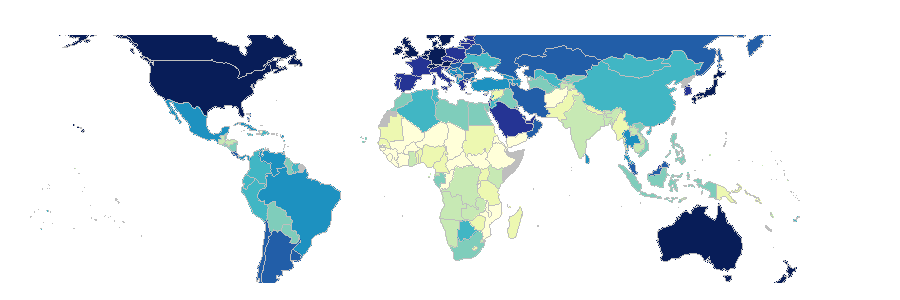
\includegraphics[width=0.9\textwidth]{world_map-HDI/world_map-HDI.pdf}
			\subcaption{Human development index by region}\label{fig:world_map-HDI}
		\end{subfigure}

		\begin{subfigure}[b]{1\textwidth}
			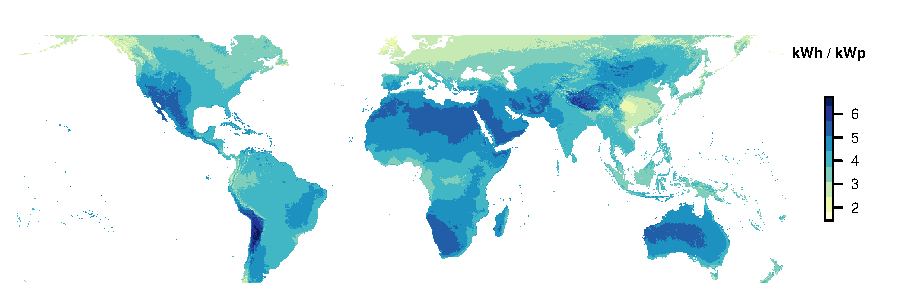
\includegraphics[width=0.9\textwidth]{world_map-PVOUT/world_map-PVOUT.pdf}
			\subcaption{Daily photovoltaic electricity potential}\label{fig:world_map-PVOUT}
		\end{subfigure}

		\begin{subfigure}[b]{1\textwidth}
			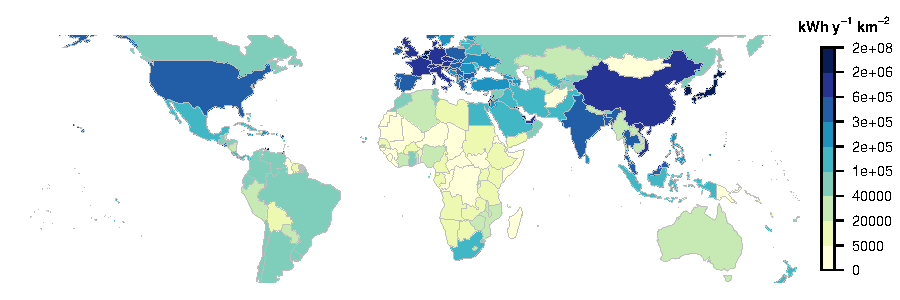
\includegraphics[width=0.9\textwidth]{world_map-electrical_vs_land/world_map-electrical_vs_land.pdf}
			\subcaption{Yearly electricity consumption over region land area}\label{fig:world_map-electrical_vs_land}
		\end{subfigure}
		\mycaption[Geographical distribution of development, sunlight and consumption.]{Data in (\textbf{a}) represent the human development index:
			"a summary measure of average achievement in key dimensions of human development: a long and healthy life, being knowledgeable and have a decent standard of living"
			from UNDP\cite{UNDP2018} (missing data in grey); data in (\textbf{b}) represents the photovoltaic electricity potential: considering a photovoltaic module installed in a region, is the ratio between the average daily produced energy, in kWh, and the nominal power, or nameplate capacity, of the installed module;\cite{Solargis2018} data in (\textbf{c}) represents the yearly electricity consumption\cite{CIAa} (comparing total electricity generated annually plus imports and minus exports) on a country scale divided by country land surface,\cite{CIA} expressed in kilowatt-hours per year per square kilometre.}\label{fig:world_map}
		}}
	\end{figure}

	\paragraph{Resilience} Photovoltaic is the electric energy production method that best matches a distributed and decentralized network model, with the only single-point-of-failure being the climate variability.
	Combined with accumulation (needed for night time usage) and with other energy sources, it can be the pivot of a completely resilient electric energy provisioning system.

	\paragraph{More energy is not enough} It is intuitive that increasing the energy production is a high-price solution to the growing energetic demand.
	Indeed, in some regions a decrease in the electricity consumption has to be included for a long-term solution.
	For example, a study\cite{Margolis2016} reports that if every rooftop (not considering utility-scale solar facilities) in United States of America was covered with solar panel, just the 39~\% of its nowadays national consumption would be covered.
	In \cref{fig:world_map-electrical_vs_land} we can see how electricity consumption density is greatly inhomogeneous and comparing with the photovoltaic potential map in \cref{fig:world_map-PVOUT}, it is evident that such a problem is shared with many other poorly insulated but energy eager regions.
	Both an increase in machinery's efficiency and a change in life-style can be part of the solution, following the example and thinking at life-style, in USA the per capita energy usage is more than twice the European average, and five times the Latin America average.\cite{IEA}

	\paragraph{And more research is needed} Every source of electrical energy we can think of works via the conversion of motive power (a flow of steam, wind, or water, waves, tides...) to electricity, which relays on the well established electric generator.
	Except photovoltaic energy.
	This very simple difference already hints for the huge conceptual and technological step required by photovoltaics as compared to other electrical energy sources.

	% transducer
	\mysection[Relevant Physics]{Relevant Physics of Stacked Semiconductor Thin Films}

	\subsection{Energy Levels and Occupancy}

		\paragraph{Valence and conduction bands}

		\paragraph{Boltzmann and Fermi-Dirac statistics}

		\paragraph{Fermi and quasi-Fermi levels}

	\subsection{Charge Generation}

		\paragraph{Light absorption}

		\paragraph{Light absorption in presence of electric field}\label{intro_electroabsorbance}

		\paragraph{Excitons and free charges generation}

		\paragraph{Hot carriers}

	\subsection{Electrostatics}

		\paragraph{Poisson equation}

	\subsection{Charge Dynamics}

		\paragraph{Charge diffusion}

		\paragraph{Charge drift}

		\paragraph{Space charge limited layers}

	\subsection{Charge Recombination}

		\paragraph{Primary geminate recombination} \label{intro_geminate} This kind of recombination happens with the annihilation of a photo-generated exciton prior to the free charges separation.
		This is independent from the illumination intensity, so it can be considered as having a reaction order of zero.
		Lead halide perovskite have quite a high static permittivity CITE IMPEDANCE and a small electron effective mass (high free carriers mobility) \cite{Herz2017}, this means that, at room temperature, the exciton binding energy is even smaller than $k_BT$ \cite{Miyata2015,Galkowski2016} and the direct generation of free charges occurs.
		So this kind of recombination is negligible in perovskite solar cells.
		%Non-geminate recombination refers to the annihilation of an electron and an hole happening after their complete separation, as opposed to geminate recombination where the recombination happens just after the charges separation but before their distancing.

		\paragraph{Radiative recombination}
		This is an unavoidable form of recombination, which finds its origin in the detailed balance principle describing that all the absorbed thermal photons have to be re-emitted as black body radiation.
		From this parallelism it can be understood that it is larger for materials with greater absorptivity \cite{Nelson2003}.
		An indirect bandgap disfavours the radiative recombination: in these materials the recombination involves a large momentum variation, while the photon emitted due to the recombination can take just a small momentum and the rest of it should be released as an additional phonon (lattice vibrations).
		Radiative recombination involves the clash of two opposite free charges, so it can be considered as having a reaction order of 2 when electrons and holes concentrations are similar, $n \approx p$ (in intrinsic semiconductors out of the depletion layer or, in intrinsic perovskites, once ionic profile stabilized cancelling the electric field), while in case of uneven concentrations (in doped semiconductors or inside depletion layers) the limiting reagent is the minority carrier (electrons in p-type and holes in n-type materials) and the reaction order is 1.
		The expression used for modelling is: $U_{rad} = k_{rad} (np-n_i^2)$, where $n_i$ is the intrinsic carrier density as obtained from Boltzmann distribution for an intrinsic semiconductor, it is just introduced in the equation in order to account for the thermal generation.

		\paragraph{SRH trap mediated recombination}
		Also known as Shockley-Read-Hall recombination \cite{Shockley1952}, this recombination happens in two steps: a free charge from the respective band decays into an empty localized state with energy in between the valence and the conduction bands, a trap, after this event, a free charge of the opposite sign reaches the trapped charge location and recombine with it.
		Usually both the momentum difference and the chemical energy get released via phonons, so no radiative emission is involved.
		This recombination type can have reaction order of 1 or of 2 depending on how many of these steps constitutes a bottleneck \cite{Calado2018b}.
		In case of mid-gap traps (with energy in the middle of the bandgap), these states will be rather saturated and the process of trapping a free charge will be slow as an empty trap has to be hit, then the actual recombination is fast, so the reaction order is 1.
		In case of shallow traps, the first step could or could not be a bottleneck, this time depending on the availability of free charges to trap: in doped semiconductors this could be a limiting factor, and the reaction order would be again 1; in intrinsic semiconductors there will be plenty of free charges of both types, and the reaction order can get close to 2.
		The expression used for modelling is \cite{Shockley1952}:
		\begin{equation}\label{eq:srh}
		U_{SRH} = k_{SRH} \frac{np-n_i^2}{\tau_n(p+p_t)+ \tau_p(n+n_t)}
		\end{equation}
		
		where $n_t$ and $p_t$ AAAAAAAAAAAAAAAAAAAAAAAAAAAAAAAAAAAAAAAA

		\paragraph{Surface recombination}\label{intro_surface_recombination}
		Also known as interfacial recombination, refers to the annihilation of one kind of free charge on a material with a charge of the opposite sign located on another material, happening at the materials' interface.
		At the interface between a, let's say, p-doped and a close-to-intrinsic material as we consider the perovskite, the surface recombination will involve the majority carrier, holes, in the doped material and the opposite charge in the intrinsic semiconductor.
		As the doped semiconductor has abundance of majority carriers, the limiting factor will be the concentration of "minority" carriers on the other side of the interface, which will depend on its mobility and on the electric field in the intrinsic.
		So the reaction order should be 1 for this case.
		The presence of mid-gap states in the doped selective contact can mediate the recombination in a fashion similar to the aforementioned Shockley-Read-Hall mechanism.
		As we will see below, this is the most important recombination pathway for perovskite solar cells.

		\paragraph{Auger recombination}
		When a free charge gets in contact with another of the same kind, it is possible that one of these decays and the other absorbs the just released energy as kinetic energy.
		This recombination is important in materials with high free carriers densities or at high photo-generation conditions.
		Additionally to the two free charges of the same kind, it also requires a free charge of the opposite kind for the decay to be possible, so it can be considered as having a reaction order of three.

	\subsection{PhotoVoltaic Effect}

		\paragraph{Charge collection}

		\paragraph{Electromotive force}

		%https://en.wikipedia.org/wiki/Electromotive_force#Solar_cell

	\subsection{Just the Needed Electrodynamics}

		\paragraph{Displacement current -- definition}\label{intro_displacement_current} The displacement current $J_D$ appears in the fourth macroscopic Maxwell's equation as $\partial D / \partial t$ for describing the contributions to magnetizing field not originated by a current of free charges $J_f$: $\nabla \times H = J_f + \frac{\partial D}{\partial t}$.
		The displacement electric field $D$ includes contributions from the electric field intensity $E$ and the polarization $P$: $D=\epsilon_0 E + P$ which can also be written in terms of relative permittivity $\epsilon_r$ as: $D= \epsilon_0 \epsilon_r E$.
		So its time derivative defining the displacement current is: $\frac{\partial D}{\partial t} = \epsilon_0 (\epsilon_r\frac{\partial E}{\partial t} + E\frac{\partial \epsilon_r}{\partial t})$.
		For the scope of this thesis we're interested in the first term and we're going to ignore the second one considering the relative permittivity as a material dependent constant.


		\begin{figure}
			\makebox[\textwidth][c]{
				\parbox{1.1\textwidth}{
					\centering
					\begin{subfigure}[t]{0.5\textwidth}
						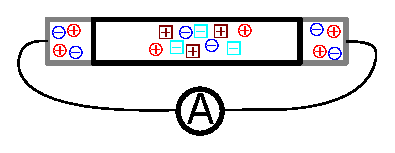
\includegraphics[width=1\textwidth]{displacement_current/first.pdf}
						\subcaption{Initial condition}\label{fig:displacement_current-initial}
					\end{subfigure}
					\bigskip

					\begin{subfigure}[t]{0.5\textwidth}
						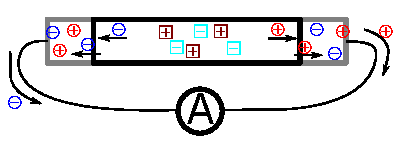
\includegraphics[width=1\textwidth]{displacement_current/second.pdf}
						\subcaption{Free charges crossing interfaces}\label{fig:displacement_current-electronic}
					\end{subfigure}
					\qquad
					\begin{subfigure}[t]{0.5\textwidth}
						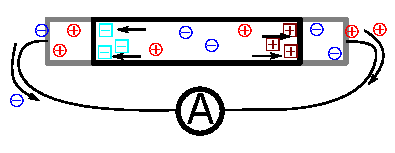
\includegraphics[width=1\textwidth]{displacement_current/third.pdf}
						\subcaption{Ionic charges accumulating at interfaces}\label{fig:displacement_current-ionic}
					\end{subfigure}

			\mycaption[Representation of current and displacement current.]{(\textbf{a}) a mixed ionic-electronic conductor material layered between two layers of electronic conductor material.
				(\textbf{b}) the electronic charge can cross the material's interfaces.
				(\textbf{c}) ionic charge cannot be transferred to the electrodes, still a displacement current due to the ionic migration is generated and can be measured in the amperometer.}\label{fig:displacement_current}
							}
			}
		\end{figure}


		\paragraph{Displacement current -- interpretation} So the displacement current accounts for the charge movements not identifiable as current and for their effect on the surrounding circuitry.
		An example is represented in \cref{fig:displacement_current-ionic}: the amperometer can measure a current even if no charge crossed the perovskite/electrode interface, this is a displacement current caused by the creation of a dipole due to the ionic accumulation at the interfaces.
		One can imagine the resulting current as needed for maintaining the zero potential difference between the two contacts.
		It is not, as one could erroneously and instinctively think, the effect of an electric field generated in the contacts by the moving charge in the perovskite layer (with related Coulomb force and image charges) as out of the two two-dimensional planes of opposed charges no electric field is present.
		This can be understood thinking that the electric field intensity generated by an large plate of charges has a constant magnitude at distances much smaller than the plate dimensions (which is always true in our solar cells considering the thickness \SI{\approx 1}{\um} to area \SI{3x3}{\square\mm} ratio, except at electrode edges).
		The concept is represented in \cref{fig:dipole_plane}.
		In \cpageref{displacement_current_ionic} we'll use the displacement current concept for simulating the current caused in the electrodes not by a net flux of charges through a device section but by the rearrangement of charges which not necessarily leave the device, like the ionic migration in perovskite material.

		\begin{figure}
			\makebox[\textwidth][c]{
				\parbox{1.1\textwidth}{
					\centering
					\begin{subfigure}[t]{0.3\textwidth}
						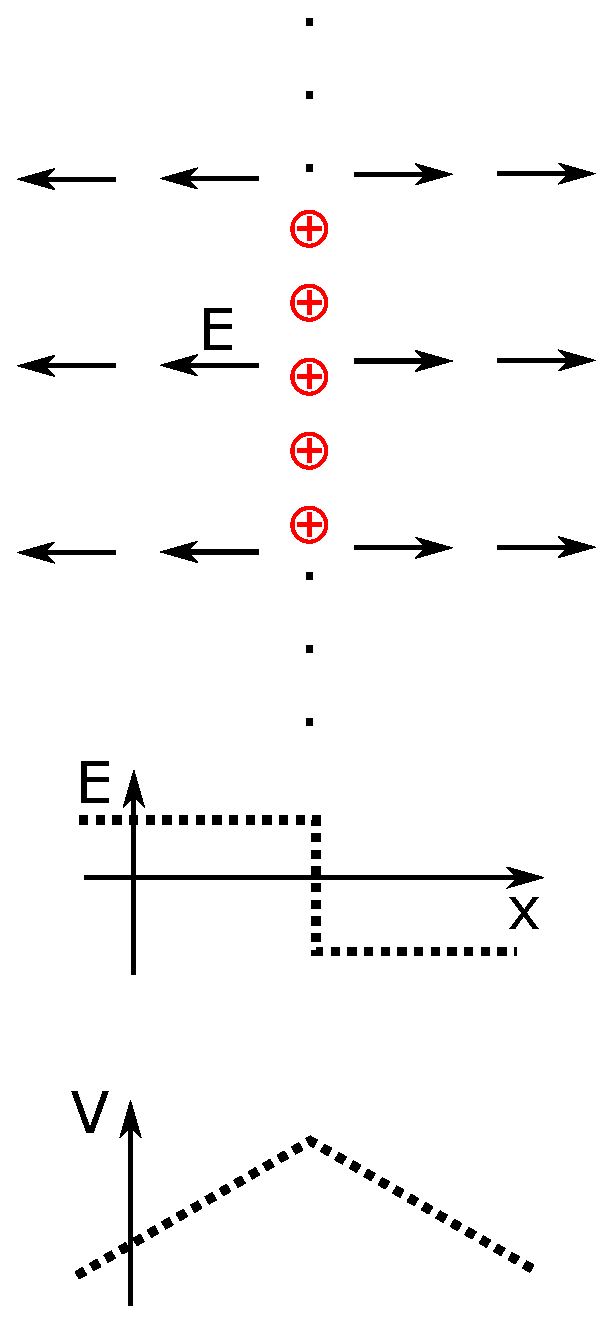
\includegraphics[height=0.3\textheight]{dipole_plane/single.pdf}
						\subcaption{Infinite plane of charges}\label{fig:dipole_plane-single}
					\end{subfigure}
					\qquad
					\begin{subfigure}[t]{0.3\textwidth}
						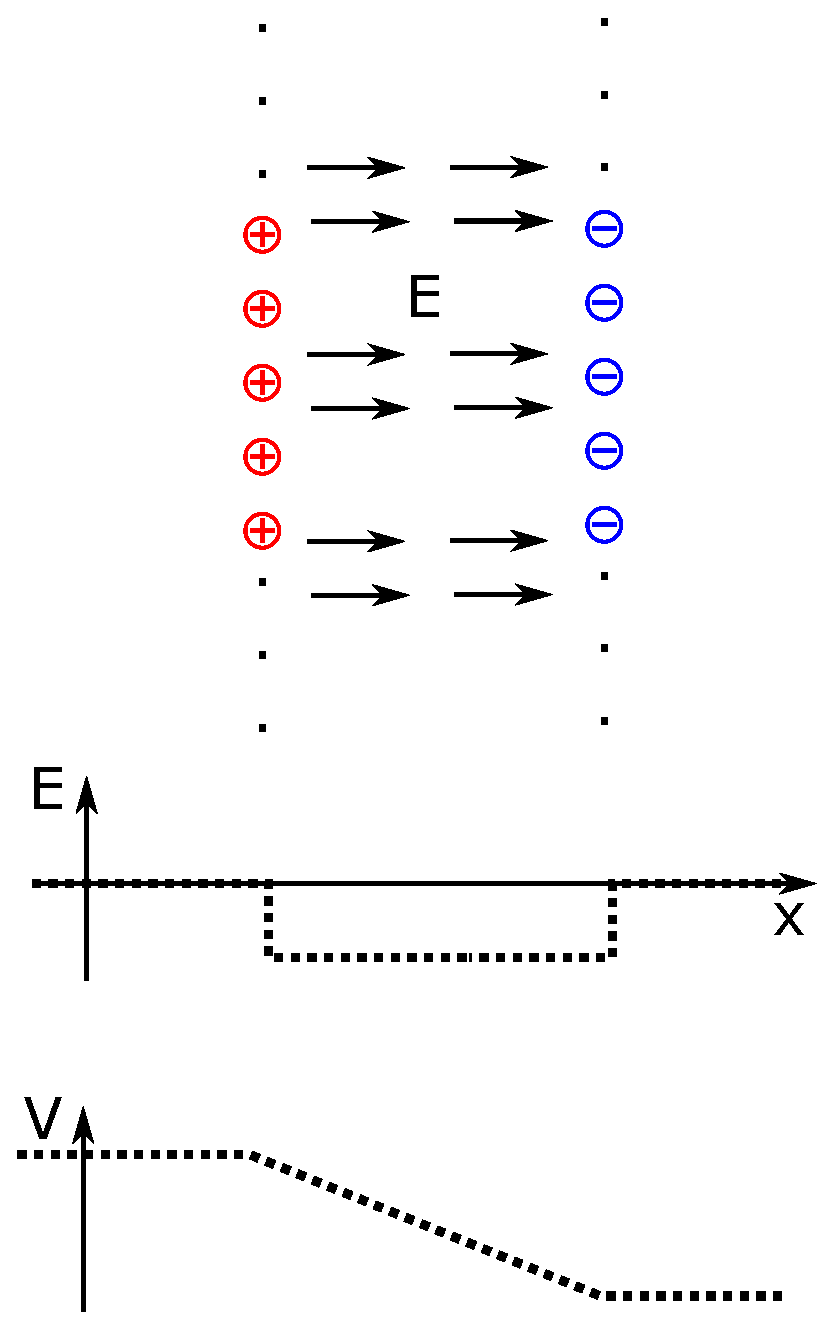
\includegraphics[height=0.3\textheight]{dipole_plane/double.pdf}
						\subcaption{Two infinite planes of opposed charges}\label{fig:dipole_plane-double}
					\end{subfigure}

			\mycaption[Electric field by two planes of opposite charges.]{(\textbf{a}) an infinite plane of charged particles is represented, the electric field is constant on the two sides, with a discontinuity in the plane.
				(\textbf{b}) adding a second plane with the same concentration of charges of the opposite kind, the electric field out of the sandwich cancels out.
				What is present outside of the sandwich is just an electrostatic potential difference.}\label{fig:dipole_plane}
							}
			}
		\end{figure}

		\paragraph{Continuity equations} The continuity equations have a very intuitive meaning: the concentration of a specie in a specific volume can increase due to generation $G$, can decrease due to recombination $U$ or can change due to a speed change of a charge flow passing by.
		This last contribution can be understood with the following example: a traffic light stops the cars flow and causes the increase of their concentration.
		For electron concentration $n$:
		$$\frac{\partial n_x}{\partial t} = \frac{1}{q}\nabla_x \cdot J_n + G_{n,x} - U_{n,x}$$

\section{Perovskite Solar Cells}

	Perovskite solar cells is a relatively new player in the photovoltaics world, existing just since 2009 (started by the research groups Miyasaka\cite{Kojima2009}, Park \cite{Im2011a,Kim2012b}, and Snaith \cite{Lee2012}).
	In relatively short time, see \cref{fig:nrel_chart}, these kind of devices reached a record stabilized efficiency of 20.9~\% \cite{Green2019} with reports of even higher non-stabilized efficiencies (23.7~\% \cite{Green2019,Jiang2017}).


	\begin{SCfigure}
		\centering
		\includegraphics[width=0.5\textwidth]{nrel_chart/pv-efficiencies-2019-01-03.pdf}
		\mycaption[NREL chart of "Best Research-Cell Efficiencies"]{Just the perovskite solar cells (not stabilized) results have been reported.}\label{fig:nrel_chart}
	\end{SCfigure}


	\paragraph{Perovskite Absorber Synthesis}
	The preparation of this hybrid semiconductor via spin coating and annealing at low temperature is extremely easy and convenient for small-scale research purposes.
	From my point of view, what most affects the perovskite research is the lack of reproducibility, likely caused by the extremely sensible crystallization during the annealing phase.
	In literature various reports of completely different results obtained from perfectly identical synthesis can be found\cite{Pockett2015,Gottesman2014}.
	This issue is being addressed recently with the publication of more reliable and complete fabrication procedures \cite{Saliba2018}.

	\paragraph{Recombination mechanisms}\label{intro_prv_recombination}
	The non-radiative recombination inside the perovskite material is surprisingly low for a low temperature processed material.
	This is demonstrated by the large diffusion length in isolated crystals \cite{Wehrenfennig2014,Wehrenfennig2014a,Stranks2013,Xing2013,Shi2015a,Eperon2014}: for the \gls{csfamapbibr} it is reported being \SI{\approx140}{\nm} for the electrons and \SI{\approx1.9}{\um} for holes \cite{Liu2017}.
	This is confirmed by the fact that once a thin layer (\SI{\approx500}{\nm}) of the material is layered between an \gls{etm} and an \gls{htm} the photoluminescence lifetime gets dramatically reduced \cite{Jimenez-Lopez2017,Eperon2014} indicating that the free charges can diffuse at least over the layer thickness.
	Even if not universally accepted \cite{Valadez-Villalobos2019}, it is often reported that in open circuit conditions, the predominant recombination pathway in perovskite solar cells is identifiable in the surface recombination at the perovskite/selective contacts interfaces \cite{Calado2018b,Stolterfoht2018a,Stolterfoht2018,Gelmetti2019,Shao2016}.
	Nevertheless, also reports on the impact of the perovskite material morphology and composition on the \gls{voc} can be found in literature: non-passivated perovskite surface states which can act as traps \cite{Zheng2017}; inhomogeneous perovskite layer can lead to pinholes \cite{Lee2015,Montcada2017,Qiu2016}; accessible grain boundaries due to non-compact perovskite layer causes the presence of more recombination centres \cite{Shao2016a}; the presence of secondary phases with in-gap energies can be reduced modifying the perovskite composition \cite{Bi2016}.

	\paragraph{Open circuit voltage}
	The open circuit voltage of a perovskite solar cell depends on many contributions, one of these is the aforementioned charge recombination velocity.
	Other important factors are: the perovskite band gap, which can be tuned changing its stoichiometry, for example partially replacing iodine with bromine \cite{McMeekin2016,Noh2013a,Wheeler2017} or using different organic cations \cite{Eperon2014}.
	This recombination is more important in a perovskite solar cell rather than in \gls{osc} as the built-in field is shielded by the ionic accumulation which increases the minority carriers concentration at the perovskite/contacts interfaces.

	\paragraph{Charge extraction and charge blocking}
	Selective contacts are in charge of selectively extract one kind of charge, blocking the other.
	Clearly, the relative position of the perovskite and selective contact energy level is key both for extraction \cite{CorreaBaena2015} and for blockage CITE SOMETHING.

	\paragraph{Ionic migration}
	The presence of charged and mobile ionic species have been demonstrated in various kind of hybrid lead halide perovskite materials, via \gls{kpfm} \cite{Birkhold2018} XXXXXXXXXXXXXXXXXX.
	The presence of mobile ions has been demonstrated also in absence of current-voltage hysteretic behaviour\cite{Calado2016,Jacobs2018}.
	It has also been demonstrated that for \gls{mapi} the majoritarian mobile species is the iodine vacancy XXXXXXXXXXXXXXXX \cite{Senocrate2017} and has been excluded a significant contribution from methylammonium ions \cite{Senocrate2018,Senocrate2017}.
	These charged species can migrate inside the material either by diffusion or when drifted by an electric field \cite{Xiao2014}.

	\paragraph{Field free absorber}
	Thanks to the abundance of the ionic specie CITATION, the electric field inside the absorber is completely shielded \cite{Tress2015}

	\paragraph{Diffusion as the main transport mechanism}(due to the built-in voltage being the workfunction difference of the selective contacts)(drift is not the main transport mechanism in stabilized perovskite solar cells due to the electric screening effect of the mobile ionic species)


	\paragraph{Hysteresis}
	It is nowadays widely accepted that hysteretic behaviour, while not so important in other kind of solar cells, it is paramount in perovskite solar cells due to the ionic migration in the absorber material \cite{Unger2014,Xiao2014}.
	The recombination and the collection of the free charges is clearly affected by the ions-modulated electric field, and this is enough to explain the presence of hysteresis \cite{Tress2015,Calado2016} via the modulation of interfacial energy barriers \cite{Moia2019}.
	Additionally, trapping or chemical reaction of perovskite ionic defects with the selective contact surface (\textit{e.g.}\ with titanium oxide \cite{Yu2016,Beilsten-Edmands2015}) could be important and can explain why \cite{Moia2019}, bottom cathode cells with inorganic contacts usually present hysteresis while top cathode with all-organic contacts usually does not.

	\paragraph{Intrinsic or doped semiconductor}


	\paragraph{Characterization}
	The characterization techniques for perovskite solar cells and the relative interpretation evolved from the techniques and theory built around \gls{osc} and \gls{dssc} \cite{Barnes2013}.
	This pre-existing framework has been widely used in literature for perovskite solar cells by various research groups \cite{ORegan2015b,Shao2016,Gelmetti2019,Kiermasch2018,Carnie2015}.
	Unfortunately, perovskite solar cells are different enough from \gls{osc} and \gls{dssc} to doom the utility of most of these observations.
	In the past few years, the theoretical framework has been expanded and should finally enable the perovskite community to re-interpret and re-design the solar cells characterization techniques.
	In \cref{ch:interpretation} the reader can find some of the accepted concepts and some novel proposals about the interpretation of the classical characterization techniques when used on perovskite solar cells.

	\paragraph{Stability}
	The stability of the perovskite solar cells is the number one blocker to commercialization.
	Its keystone has still to be identified.
	An interesting investigation is being carried on by D.\ R.\ Ceratti and D.\ Cahen (unpublished) regarding the release of a proton by methylammonium cation when in contact with non-acidic materials, and thus leaving the perovskite crystal structure.
	This could explain the reports about the beneficial addition of acids in perovskite precursors solution, mainly by Snaith group \cite{Noel2017,Zhang2015a,Nayak2016}.


	https://www.ossila.com/pages/perovskite-solar-cell-degradation-causes




	Influence of perovskite material on Voc \cite{Wheeler2017,Eperon2014,Noh2013a}

	Influence of contacts on Voc \cite{CorreaBaena2015} WU2016A

\section{Background and Related Work}\label{sec:background}

	\subsection{Perovskite Solar Cells}

	\subsection{Hole Transporting Materials}

	\subsection{PhotoPhysical Studies and Techniques}

	\subsection{Modelling and Relevant Physics}

	\clearpage
	\stopcontents[intro]

\chapter{Experimental Methods}\label{ch:methods}
\chaptermark{Experimental Methods}
	\epigraph{\textit{"When it's a humid day, we don't fabricate cells"\\"But\dots  don't you fabricate them in a glovebox?"\\"Of course."}}

	\addthumb{\thechapter}{\LARGE{\textbf{\textrm{\thechapter}}}}{white}{colortwo}
	

	\paragraph*{Abstract} The experimental methods are described here in detail, mixed with comments and warnings to the reader, trying to underline the critical points spotted over my PhD.
	Needless saying, the critical points in fabricating a complex electronic device such as a perovskite solar cells are many and neither a proper description can assure reproducibility.
	
\newpage
%Important to finish this paragraph, for example with an empty line for avoiding the following error:
% .ptc Something's wrong--perhaps a missing \item. ...rline {4.1}Introduction}{89}{section.4.1}
	\centerline{\rule[0.5ex]{0.2\linewidth}{1pt} \textbf{Table of Contents} \rule[0.5ex]{0.2\linewidth}{1pt}}
	
	\startcontents[methods]
	\printcontents[methods]{l}{1}{\setcounter{tocdepth}{4}}

	\centerline{\rule[0.5ex]{0.5\linewidth}{1pt}}

	\graphicspath{ {./contents_img/methods/} }

	\newpage
	


\section{Materials}
	Dust free cloths Super Polx 1200A \SI{23x23}{\cm} were bought from Berkshire.

	Patterned \gls{fto} substrates with sheet resistance of \SI{7}{\ohm\per\sq} (TEC7) on \SI{2.2}{\mm} thick and \SI{14.8x14.8}{\mm} wide Pilkington glass were bought from Xinyan Technology Ltd.

	Patterned \gls{ito} substrates with sheet resistance of \SI{15}{\ohm\per\sq} on \SI{1.1}{\mm} thick and \SI{15x15}{\mm} wide glass were bought from Xinyan Technology Ltd.

	All anhydrous and non-anhydrous solvents had a reagent grade purity; were purchased from Sigma-Aldrich and used without any additional treatment.

	Titanium(IV) isopropoxide (97~\%), acetylacetone, and \glsdesc{litfsi} (\gls{litfsi}) were bought from Sigma-Aldrich.

	\Gls{pedotpss} Clevios P VP.AI 4083 was bought from Heraeus.

	\ch{PbI2} (99~\%), \ch{PbBr2} (99.999~\%), \ch{CsI} (99.999~\%), \ch{PbCl2} (98~\%), anhydrous chlorobenzene, anhydrous \gls{dmf}, and anhydrous \gls{dmso} were bought form Sigma-Aldrich and kept in a nitrogen-filled glovebox.

	Methylamine in methanol (40~w/w\%, \SI{\approx9.8}{\Molar}) was bought from Tokyo Chemical Industry.

	\Gls{fai}, \gls{mabr} and \gls{mai} were either synthesized (described in \cpageref{methods-MAI}) or bought from GreatCell Solar (unknown purity).

	4-tert-butylpyridine and hydroiodic acid (57~m/m\% in water) were bought from Sigma-Aldrich and kept in a fridge (the colour of both these reagents change with ageing when kept out of the fridge, indicating degradation).

	\Gls{spiro} was bought from 1-Material and stored in a nitrogen-filled glovebox.

	\Gls{tae1}, \gls{tae3}, and \gls{tae4} molecules (subject of the study in \cref{ch:tae}) were used as received from Dr.\ Inés García-Benito, Dr.\ Agustín Molina-Ontoria and Dr.\ Nazario Martín (IMDEA, Madrid).
	The synthesis of \gls{tae1} has been described in \authoryear{Cabau2015a} and \authoryear{Choi2015b}.
	The synthesis of \gls{tae3} and \gls{tae4} has been described in \authoryear{Gelmetti2019}.

\section{Equipments}

	\subsection{Equipments for Fabrication}

		\paragraph{Ultra-violet ozone cleaning system}
		Organic residuals removal was performed with a T10X10/OES UV/ozone cleaning system from UVOCS.
		Most common failure: insufficient gas extraction flow detected by differential pressure meter on the rear, it can be partially configured \textsl{via} a screw.
		It has been used for the treatment of \gls{fto} and \gls{ito} just prior to the deposition of titanium oxide precursors or \gls{pedotpss}.
		For the latter, this process improves the \gls{pedotpss} coverage increasing the support hydrophilicity.

		\paragraph{Spin coater in air atmosphere}
		Spin coating depositions in the clean room were performed with a Laurell WS-400BZ-6NPP-LITE spin coater.
		It has been used for deposition of titanium oxide precursors, \gls{pedotpss}, \gls{pcbm60}, and \gls{pcbm70}.

		\paragraph{Muffle oven}
		Calcination was performed with a muffle oven Hobersal HD-230 controlled with a Fuji Electric PXR-4.
		Most common failure: misuse of the controller by the users can cause unexpected excessive heating.
		It has been used for calcination of just-deposited dense titanium oxide thin films.

		\paragraph{Titanium hotplate}
		Calcination can be performed with a titanium hotplate Harry Gestigkeit PZ 28-3TD.
		Most common failures: controller failure and heating resistance breaks in a point, it can be unmounted and replaced.
		It has been used for calcination as an alternative to muffle oven.

		\paragraph{Glovebox}
		Perovskite deposition and precursors storage was done in a nitrogen-filled glovebox MBraun UNILab.

		\paragraph{Spin coater in inert atmosphere}
		Spin coating depositions in the nitrogen-filled glovebox were performed with a SPIN150 equipment (this model does not require a gas inlet, which would be troublesome in a glovebox) from SPS Europe where the transparent cap was removed from the lid for helping solvent vapours removal.
		For avoiding the accumulation of waste material, an aluminium foil was used for covering the deposition chamber and was replaced frequently.
		Most common failure: exhaustion of the supposedly \SI{20}{\year} lasting non-volatile SRAM (integrated circuit BattRam DS1230Y-85+ DIP28, a perfect example of planned obsolescence).
		It has been used for depositing the perovskite precursors and the \gls{htm} selective contacts.

		\paragraph{Precision hotplate}
		Annealing was performed with a highly homogeneous hotplate JP Selecta Plactronic.
		It has been used for annealing the just-deposited perovskite thin films.

		\paragraph{Thermal evaporator}
		High vacuum (\SI{1E-9}{\bar}) thermal depositions were performed with a MBraun vacuum deposition chamber connected with a scroll pump in series to a turbo pump.
		The deposition was controlled with an Inficom SQC310C unit (firmware version 6.44).
		The deposition rate was measured \textsl{via} two oscillating quartz sensors whose calibration tooling was performed yearly.
		The evaporation chamber was embedded in a MBraun MB200B glovebox module controlled by a MBraun MB20G.
		%inorganic and metallic materials%while the organic material deposition was controlled in a manual fashion with a CreaPhys temperature control unit CU~103
		It has been used for depositing the metallic electrodes, usually gold or silver.

	\subsection{Equipments for Materials Characterization}

		\paragraph{Optical microscope}
		Optical microscopy images were acquired with a Leica S6 D microscope.
		It has been used for studying the homogeneity of the deposited thin films.

		\paragraph{UV--Vis--NIR spectrophotometer}
		Absorbance measurements were carried out on a Lambda 1050 PerkinElmer spectrophotometer equipped with a PhotoMultiplier Tube, \ch{InGaAs} and \ch{PbS} detectors system, double beam optics, double monochromator, \ch{D2} and \ch{W} light sources.
		It has been used for estimating the thickness of the deposited thin films.

		\paragraph{PhotoLuminescence spectrophotometer}
		Fluorescence measurements were carried out on a Fluorolog Horiba Jobin Yvon spectrofluorimeter equipped with photomultiplier detector, double monochromator, and Xenon light source.
		It has been used for the characterization of molecules in solution.

		\paragraph{Time Resolved PhotoLuminescence spectrophotometer}
		PhotoLuminescence lifetime measurements were carried out on a Edinburgh Instruments LifeSpec-II based on the \gls{tcspc} technique, equipped with a PhotoMultiplier Tube detector, double subtractive monochromator and picosecond pulsed diode lasers source.
		It has been used for comparing the radiative recombination life-time in perovskite thin films with or without selective contacts.

		\paragraph{X--ray diffractometer}
		\gls{xrd} measurements were made using a Bruker-AXS D8-Discover diffractometer equipped with parallel incident beam (Göbel mirror), vertical $\Theta$~-~$\Theta$ goniometer, XYZ motorized stage and with a GADDS (General Area Diffraction System).
		Samples were placed directly on the sample holder and the area of interest was selected with the aid of a video-laser focusing  system.
		An X-ray collimator system allows to analyse areas of \SI{500}{\um}.
		The X-ray diffractometer was operated at \SI{40}{\kV} and \SI{40}{\mA} to generate \ch{Cu} K$\alpha$ radiation.
		The GADDS detector was a HI-STAR (multiwire proportional counter of \SI{30x30}{\cm} with a \SI{1024x1024}{pixel}).
		We collected frames (2D \gls{xrd} patterns) covering \SIrange{15}{70}{\degree} $2\Theta$ from three different detector positions at a distance of \SI{15}{\cm} from the sample.
		The exposition time was \SI{300}{\s} per frame and it was chi-integrated to generate the conventional $2\Theta$ \textsl{versus} intensity diffractogram.
		Identification of the materials was achieved by comparison of the \gls{xrd} diffractogram with the ICDD data base (release 2007) using Diffracplus Evaluation software (Bruker 2007).
		It has been used for investigating the chemical composition of perovskite thin films after some months in contact with organic molecules.

		\paragraph{\Acrshort{esem} and \acrshort{esem}-\acrshort{edx} microscopes}
		Superficial and cross section \gls{esem} images were acquired at low voltage (beam accelerated with \SI{20}{\kV}) and high vacuum (\SI{1E-8}{\bar}) in a FEI Quanta 600 FEG microscope.
		The cut for cross section was performed mechanically: a small angle grinder (from Dremel) was used for furrowing a diagonal line on the substrate glass side (opposite to the \gls{fto}), then using two pliers the substrate was forced as if it was to bend the glass and opening further the furrow.
		It has been used for studying the homogeneity of the thin film coverage both from the top view and from the cross section.

		\paragraph{\Acrshort{afm} microscope}
		The \acrfull{ac-afm} imaging was done \textsl{via} \gls{afm} (Pico SPM II) and processed with WSxM software \cite{Horcas2007}.
		It has been used for confirming the coverage of the deposited thin films and for measuring their roughness.

		\paragraph{Profilometer}
		Thicknesses were measured furrowing layers with a hard object and measuring the elevation profile with an Ambios Tech.\ XP-1 profilometer.
		It has been used for measuring the thickness of the deposited layers thicker than \SI{100}{\nm}.

	\subsection{Equipments for Devices Electrical Characterization}

		\paragraph{Devices holder}
		The devices holder is designed for holding 4 devices with 4 independent diodes each (the bottom electrode electrical contact is in common for all the diodes, the top electrodes contacts are independent) and consists in an airtight container topped with a quartz window.
		It was designed and fabricated by Ikerlan.
		The holder has at least one gold tip for each diode's electrode, the contact is ensured by springs pushing the tips towards the devices.
		A printed circuit board connects the gold tips to a coaxial connector \textsl{via} two rotatory selectors which allows to select the needed diode.
		It has been used for contacting the electrodes of the devices during all electrical measurements.

		\paragraph{Solar simulator}\label{solarsimulator}
		The illumination with accurate solar spectra was provided by a Sun 2000 solar simulator (\SI{150}{\W}) bought from ABET Technologies.
		The proper filters of the lamp were set to simulate the AM 1.5G solar spectrum.
		The light intensity at the measurement position was measured via the short circuit current of a small photodiode calibrated with a certified (NREL) silicon photodiode and regulated to \SI{1000}{\W\per\m\squared}.
		When needed, the light intensity was reduced using neutral filters.
		Most common failure: the power supply providing high voltage to the lamp.
		It has been used for illuminating the devices during current-voltage sweeps.

		\paragraph{Programmable digital multimeter}
		Currents and voltages were performed with a Tektronix Keithley 2400 (firmware revision C30) programmable digital source meter connected to a computer \textsl{via} a GPIB-USB-HS adapter from National Instruments, connected to the solar simulator for the shutter control \textsl{via} a RS-232 (Keithley side) to coaxial (solar simulator side), and connected to the device to measure \textsl{via} a coaxial (devices side) to 2 banana plugs (Keithley side).
		Most common failure: we observed sparks in the devices when connecting to the Keithley multimeter, so from our experience we recommend to manually set the Keithley in current measure mode with zero applied voltage, start the measure with the device not connected and finally connect the device.
		It has been used for registering the current-voltage sweeps.

		\paragraph{White \gls{led} illumination}
		White illumination at tunable intensity was provided \textsl{via} a white light \gls{led} ring with \gls{led} from LUXEON Lumileds and powered by a Aim-TTi PLH120-P power supply.
		It has been used for background illumination for \acrfull{ce}, \acrfull{tpv}, or \acrfull{tpc} measurement.

		\paragraph{Pulsed illumination}
		Perturbation illumination for photophysical characterization was provided by a nanosecond PTI GL-3300 nitrogen laser.
		The pulse was triggered with a Aim-TTi TG330 analog function generator generating a square wave pulse.
		The pulse duration is around \SI{1.5}{\ns}.
		The wavelength was selected using the absorption and emission of a dissolved molecular dye.
		The pulse intensity was attenuated with a semi-transparent glass for ensuring the small perturbation regime.
		The equipment can output up to 20~pulses per second, but due to the oscilloscope internal memory speed we're limited to 1~pulse per second.
		It has been used for providing the illumination perturbation in \acrshort{tpv} characterization.

		\paragraph{Oscilloscope}
		The voltage transients for photophysical characterization were registered with a Yokogawa DLM2052 oscilloscope with an internal resistance of \SI{1}{\mega\ohm}, connected to the device holder \textsl{via} coaxial cable and to a computer \textsl{via} an USB2 port (the transfer speed could be better if an Ethernet connection were used).
		For each registered transient, \SI{12500}{points} were saved (the maximum record length for this oscilloscope is \SI{125}{Mpoints} and the maximum sampling rate is \SI{2.5}{Gpoints\per\s}).
		It has been used for measuring the voltage transients for the \acr{tpv}, \acr{tpc}, and \acr{ce} measurement.

		\paragraph{Switch for transient measurements}
		An equipment built in-house was used as a switch for opening and closing connections based on the input from a Aim-TTi TGP110 pulse generator.
		It has been used for simultaneously shutting down the white \gls{led} ring and short the devices during the \acr{ce} measurements.

		%FT-IR ATR
		%CycloVoltammetry CH instruments electrochemical workstation CHI660C
		%IPCE
		%red and blue LEDs
		%TAS
		%TEM
		%raman

\section{Synthesis, Handling and Purification}

	\subsection{\Glsentrytext{mai} Synthesis}\label{methods-MAI}

		%Reference in laboratory notebook: [ig15, ig18, ig31, ig83].

		\ch{CH3NH2 + HI\aq -> CH3NH3I\sld}

		The synthetic method was inspired by \cite{Im2011a}.
		In a \SI{500}{\ml} one-necked flask (over-dimensioned for easing the drying step) opened at air, \SI{14}{\ml} of a methylamine in methanol (\SI{40}{w/w\%}, \SI{\approx9.8}{\Molar}) were introduced.
		While stirring and cooling at \SI{0}{\celsius}, \SI{15}{\ml} of hydroiodic acid in water (\SI{57}{w/w\%}) was added drop-wise.
		The cooling was interrupted and the mixture was continuously stirred at room temperature.
		Then the vessel was left still overnight.
		The solution was evaporated in a vacuum-assisted rotatory evaporator at \SI{60}{\celsius}.
		The obtained white solid was scraped and transferred on a funnel with membrane filter (Sartorius, \gls{ptfe}).
		It was washed with diethyl ether and the diethyl ether discarded.
		The solid was dissolved with ethanol, using as little volume as possible and vacuum was used for forcing the ethanol through the filter.
		The solid was recrystallized pouring abundant diethyl ether, then filtered, washed with diethyl ether and dried at vacuum overnight.

	\subsection{Lead Salts Handling}

		Lead iodide and bromide bottles have to be opened in a nitrogen-filled glovebox.
		The failure in keeping the lead containing precursors away from oxygen causes the formation of insoluble derivatives, likely lead oxide or metallic lead, which will have to be filtered away from the precursors solution.

	\subsection{Dense Titania Precursors Solution}\label{precursors_tio2}

		The precursor solution for the dense \ch{TiO2} layer was prepared adding drop-wise \SI{0.38}{\ml} of acetylacetone to \SI{0.65}{\ml} of \iupac{titanium(IV) isopropoxide} and diluted in \SI{5}{\ml} of ethanol.
		Beware that the titanium-acetylacetone reaction is strongly exothermic.
		The solution can be used just for a few days after preparation.
		Some hydrolysed product can be present in the solution, so it has to be filtered (\gls{ptfe}, \SI{0.2}{\um}) just before the usage.

		An alternative synthetic route has been recently employed, starting from the stable and commercially available \iupac{titanium diisopropoxide bis(acetylacetonate)} as a convenient alternative: \SI{220}{\ul} of \ch{Ti(i-PrO)2(acac)2} in isopropanol (\SI{75}{w/w\%}, \SI{0.45}{\mmol}) were diluted adding \SI{1.28}{\ml} of isopropanol and filtered (\gls{ptfe}, \SI{0.2}{\um}) just before the usage.

	\subsection{\Glsentrytext{mapicl} Perovskite Precursors Solution}\label{precursors_mapicl}

		%The solution was prepared in the laboratory.
		In a vial, \SI{400}{\mg} of \gls{mai} (\SI{2.52}{\mmol}) and \SI{230}{\mg} of \ch{PbCl2} (\SI{98}{\%}, \SI{0.81}{\mmol}) were weighted.
		Then \SI{1}{\ml} of anhydrous \gls{dmf} was added and the solution was stirred at \SI{65}{\celsius} for \SI{1.5}{\hour}.
		The solution was not filtered and was used the same day of preparation.

	\subsection{\Glsentrytext{csfamapbibr} Perovskite Precursors Solution}\label{precursors_csfamapbibr}

		In a nitrogen-filled glovebox, \SI{507}{\mg} of \ch{PbI2} (\SI{99}{\%}, \SI{1.1}{\mmol}), \SI{73.4}{\mg} of \ch{PbBr2} (\SI{99.999}{\%}, \SI{0.200}{\mmol}), \SI{172}{\mg} of \gls{fai} (\SI{1.00}{\mmol}) and \SI{22.4}{\mg} of \gls{mabr} (\SI{0.200}{\mmol}) were weighted and mixed in a \SI{5}{\ml} vial.
		For reducing the effect of static charging on the weighting process in the glovebox, a stainless steel weighing boat was specifically fabricated.
		The mixed solid precursors can show some darkening due to the formation of perovskite in a solid-solid reaction (also known as mechanosynthesis \cite{Prochowicz2018}), nevertheless this solid mixture can be stored in the glovebox for weeks.

		The day of the deposition, \SI{0.2}{\ml} of anhydrous \gls{dmso} and \SI{0.8}{\ml} of anhydrous \gls{dmf} were added to the solid mixture of precursors.
		The solution was vigorously stirred at \gls{rt} for \SI{1}{\hour}.
		Heating or storing the solution for days has been observed to result in a yellow perovskite layer when deposited and annealed, so some kind of detrimental transformation is evident to happen in the solution, hindering its storage for long time.
		Finally \SI{42}{\ul} of	a \SI{1.5}{\Molar} \ch{CsI} solution in \gls{dmso} (\SI{63}{\umol}) were added to the previous solution.
		The solution was filtered (\gls{ptfe}, \SI{0.2}{\um}) just before its usage.
		The resulting stoichiometry is \ch{Cs_{0.06}FAMA_{0.2}Pb_{1.3}I_{3.2}Br_{0.6}}.

	\subsection{\Gls{spiro} and Other \glsentryshort{htm} Solutions}

		\paragraph{Additives mother solution}
		A solvent with additives mix was prepared adding \SI{197}{\umol} of 4-tert-butylpyridine (\SI{28.8}{\ul}) to \SI{1}{\ml} of anhydrous chlorobenzene, then \SI{32}{\umol} of \glsdesc{litfsi} (\gls{litfsi}, \SI{9.1}{\mg}) were added.
		The presence of 4-tert-butylpyridine enables the solubility of \gls{litfsi} in chlorobenzene (otherwise it would have to be dissolved in acetonitrile).

		\paragraph{\Gls{spiro}}
		\Glsdesc{spiro} solution was prepared dissolving \SI{59.0}{\umol} of \gls{spiro} (\SI{72.3}{\mg}) in \SI{1}{\ml} of the aforementioned solvent with additives mix.

		\paragraph{TAE-*}
		Other \gls{htm} solutions for bottom cathode cells were prepared dissolving either \SI{29.5}{\umol} of \glsdesc{tae1} (\gls{tae1}, \SI{36.6}{\mg}), \SI{19.7}{\umol} of \glsdesc{tae3} (\gls{tae3}, \SI{24.4}{\mg}), or \SI{9.83}{\umol} of \glsdesc{tae4} (\gls{tae4}, \SI{12.1}{\mg}) in \SI{1}{\ml} of solvent with additives further diluted with chlorobenzene in a 1:1, 1:2, 1:5 ratio respectively, in order to preserve the \gls{htm} to additives molar ratio of the \gls{spiro} solution (roughly \SI{3}{\eq} of 4-tert-butylpyridine and \SI{0.5}{eq} of \gls{litfsi}).
		The lower concentrations were used due to the lower solubility of these \gls{htm} as compared to \gls{spiro} one.

		\paragraph{Oxidation control}
		The \gls{spiro}, \gls{tae1}, \gls{tae3}, and \gls{tae4} solutions did not include chemical oxidizing agents and were prepared in a nitrogen-filled glovebox in order to have control over the oxygen oxidation degree of the molecules.

		\paragraph{\Gls{pedotpss}}
		\Glsdesc{pedotpss} (\gls{pedotpss}) was used as received from the commercial supplier.

		\FloatBarrier
		\newpage
\section{Perovskite Solar Cells Fabrication}
	\epigraph{\textit{\enquote{Making good devices is an art}}}

	The "top" or "bottom" naming refers to the cell orientation during fabrication, so the "bottom" layer is the one closer to the glass substrate, as shown in \cref{fig:device_naming}.
	Both the top and the bottom cathode solar cells were fabricated following the scheme reported in \cref{fig:device_layout}.

	\begin{figure}
		\makebox[\textwidth][c]{
			\parbox{1.1\textwidth}{
				\centering
				\begin{subfigure}[t]{0.61\textwidth}
					\centering
					%					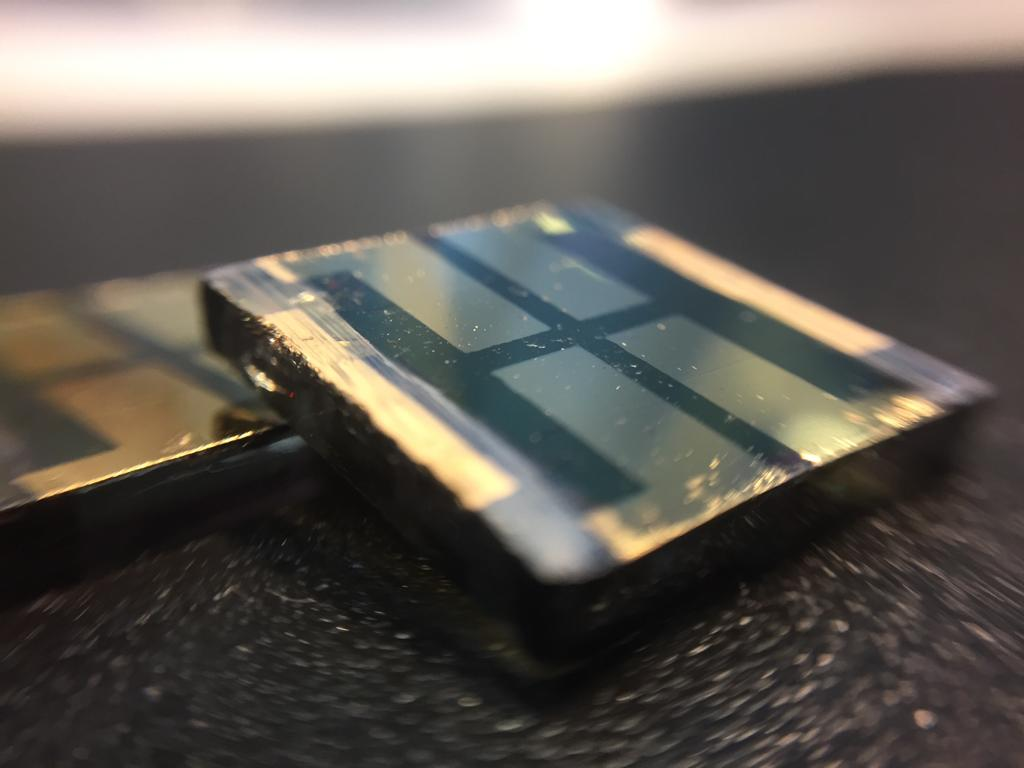
\includegraphics[width=0.4\textwidth]{device_picture/Perovskite_Palomares_ICIQ.jpeg}
					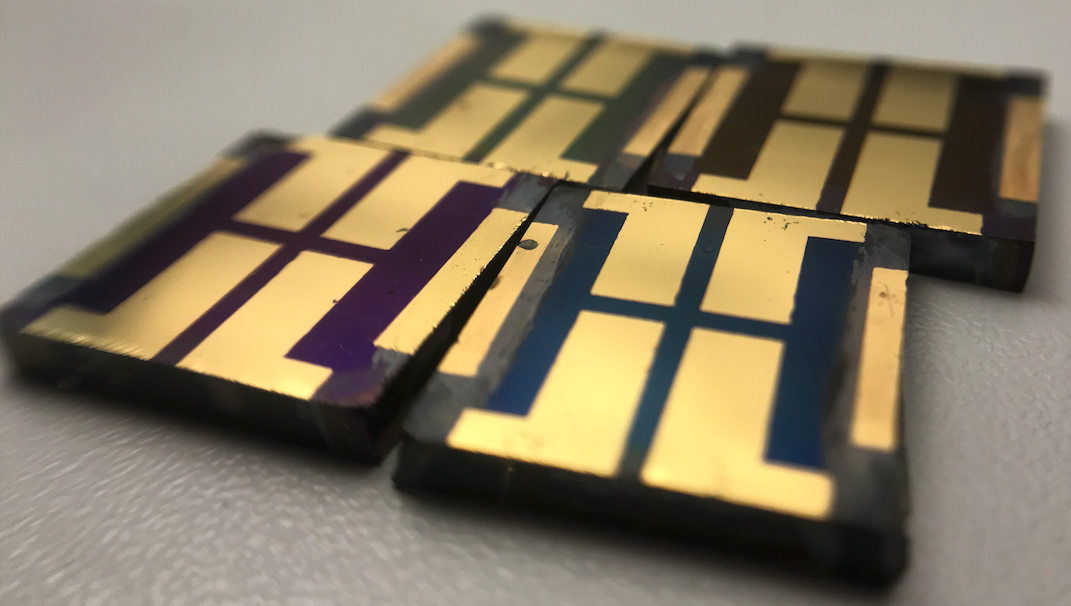
\includegraphics[width=0.8\textwidth]{device_picture/iciq_tae_news-crop.jpg}
					\subcaption{Bottom cathode perovskite solar cells}\label{fig:device_picture}
				\end{subfigure}
				\qquad
				\begin{subfigure}[t]{0.41\textwidth}
					\centering
					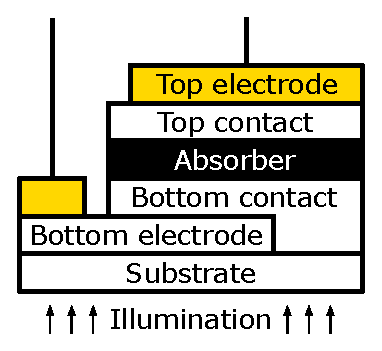
\includegraphics[width=0.9\textwidth]{bottom_top_naming/bottom_top_naming.pdf}
					\subcaption{Solar cell stack layers}\label{fig:device_naming}
				\end{subfigure}
				\bigskip

				\begin{subfigure}[t]{1.1\textwidth}
					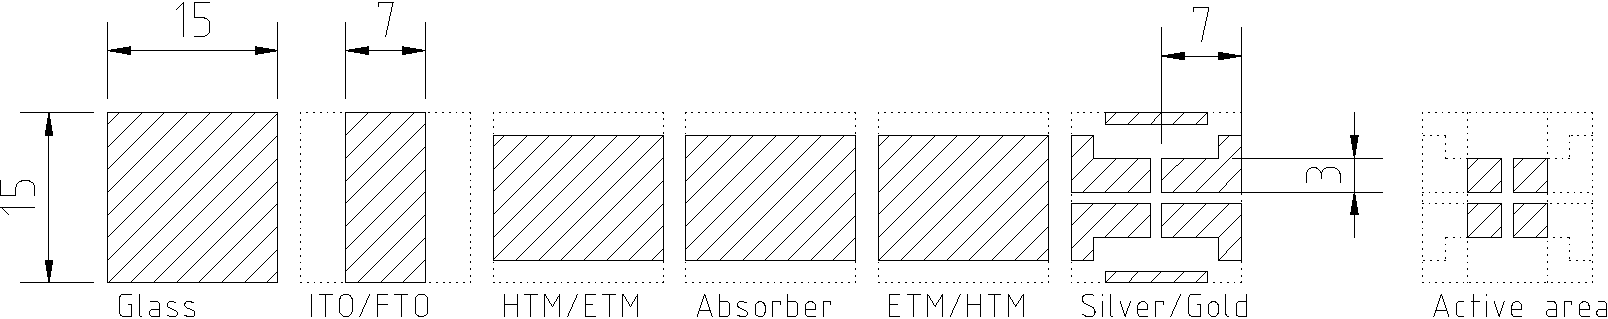
\includegraphics[width=1\textwidth]{device_layout/device_layout-crop.pdf}
					\subcaption{Schema of the layers}\label{fig:device_layout}
				\end{subfigure}

				\mycaption[Solar cells layers layout.]{
					In (\textbf{a}) a picture of typical bottom cathode perovskite solar cells is reported, each cell have a different \gls{htm} \cite{Gelmetti2019}.
					In (\textbf{b}) "top and bottom" naming is represented.
					The layers are named in the fabrication order, from the substrate up.
					The selective \gls{htm} and \gls{etm} contacts are named "contacts" just for brevity.
					The non-selective electrodes used for the electric connections are referenced as "electrodes".
					In (\textbf{c}) the shapes and dimensions of the utilised layers for top/bottom cathode solar cells are shown.
					From left to right: the glass substrate, the bottom transparent conducting oxide electrode, the bottom selective contact, the absorber, the top selective contact, the top metallic electrode.
					The active area is defined by the overlap of the \gls{ito}/\gls{fto} and the silver/gold layers, being \SI{9}{\square\mm}.}\label{fig:device}
			}
		}
	\end{figure}

	\FloatBarrier
	\subsection{Top Cathode Perovskite Solar Cells}\label{methods_top}

		\begin{SCfigure}
			\centering
			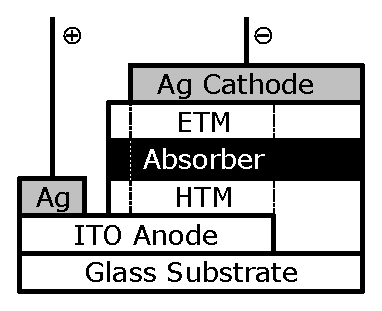
\includegraphics[width=0.4\textwidth]{bottom_top_cathode/top_cathode.pdf}
			\mycaption[Top cathode solar cell.]{The stack of a top cathode solar cell.
				The shapes dimensions does not relate to real thicknesses and areas.
				The dashed lines indicate the active area.}\label{fig:top_cathode}
		\end{SCfigure}

		\paragraph{Anode and \gls{htm} substrate reparation}
		% based on ig77
		This process was performed in a ISO~7 clean room.
		\Gls{ito} coated substrates were cleaned in an ultrasound bath with acetone for \SI{15}{\min}, isopropanol for \SI{15}{\min} and rubbed with a dust-free cloth.
		Finally, an UV/ozone treatment was performed for \SI{20}{\min}.
		\Gls{pedotpss} was filtered on \gls{pes} membrane (\SI{0.22}{\um})
		and deposited via spin coating (static dispensing, \SI{110}{\ul}) with a first step where the speeds regulates the thickness of the layer and a second step for removing the residual liquid accumulated at the substrate corners.
		The conditions are reported in \cref{table:pedotpss_thickness} and the thicknesses were obtained \textsl{via} absorbance of light with wavelength \SI{2150}{\nm} calibrated to the a very thick layer measured with the profilometer.
		A rough relation between the thickness $d$ and the spinning speed $f$ (with \SI{1000}{\rpm\per\s} acceleration) was found as $d = \frac{1820}{\sqrt{f}}$.
		Substrates were dried at \SI{110}{\celsius} for \SI{20}{\min} and stored in a nitrogen-filled glovebox for avoiding moisture absorption.

		\begin{table}%[h]
			\caption{\Glsentrytext{pedotpss} deposition conditions and resulting thickness}\label{table:pedotpss_thickness}
			\begin{center}
				\begin{tabular}{c c c | c c c | c}
					\multicolumn{3}{c|}{\textbf{\nth{1} step}} & \multicolumn{3}{c|}{\textbf{\nth{2} step}} & \multirow{2}{*}{\textbf{thickness}}                                                                    \\
					acceleration                               & speed                                      & time                                & acceleration        & speed         & time        &              \\
					$[\si{\rpm\per\s}]$                        & $[\si{\rpm}]$                              & $[\si{\s}]$                         & $[\si{\rpm\per\s}]$ & $[\si{\rpm}]$ & $[\si{\s}]$ & $[\si{\nm}]$ \\[1mm]
					\hline
					\rule[0ex]{-4pt}{3ex}
					1000                                       & 1000                                       & 60                                  & 2000                & 2000          & 3           & 65           \\
					1000                                       & 1600                                       & 60                                  & 2000                & 2000          & 3           & 45           \\
					1000                                       & 4500                                       & 30                                  & 500                 & 3500          & 30          & 27           \\
				\end{tabular}
			\end{center}
		\end{table}

		\paragraph{\Acr{mapicl} perovskite one step fabrication}
		% ig71
		The deposition process was performed in a nitrogen-filled glovebox.
		The precursors solution (see \cpageref{precursors_mapicl}) was deposited \textsl{via} spin coating (\SI{80}{\ul}, static dispensing, loading time \SI{5}{\s}) with an acceleration of \SI{1000}{\rpm\per\s}, a speed of \SI{1900}{\s} for \SI{40}{\s}.
		The substrate was moved directly to a hotplate at \SI{100}{\celsius} and annealed for \SI{80}{\min}, resulting in a \SI{430}{\nm} thick perovskite layer.
		The film is colourless just after deposition, then it turns to brown, yellow and finally black on the hotplate.

		\FloatBarrier
		\paragraph{\Acr{mapi} perovskite two step fabrication}
		% based on ig79
		This process was performed in a nitrogen-filled glovebox.
		A constant purge of glovebox atmosphere is needed during the whole deposition process.
		This reduces the \gls{dmf} and \gls{dmso} vapours concentration avoiding damages to the formed perovskite layer and the poisoning of the glovebox oxygen removal catalysts.
		\SI{460}{\mg} of \ch{PbI2} were dissolved in \SI{1}{\ml} of a 23:2~v/v blend of anhydrous \gls{dmf} and anhydrous \gls{dmso}.
		This solution was stirred at \SI{50}{\celsius} for \SI{1}{\hour}.
		\SI{50}{\mg} of \gls{mai} were dissolved in \SI{1}{\ml} of a 3:1~v/v blend of anhydrous isopropanol and ethanol.
		A \ch{PbI2} layer was deposited from the unfiltered solution via spin coating (static dispensing, \SI{80}{\ul}, loading time \SI{5}{\s}) with accelerations and speeds reported in \cref{table:mapi_thickness}.
		After \SI{60}{\s} from the start of the spin coating, the \gls{mai} solution (\SI{100}{\ul}) was dynamically dispensed on the centre of the spinning substrate with a \SI{100}{\ul} micropipette keeping it tilted and depositing an uninterrupted stream.
		The substrate was then moved directly from the spin coater to a hotplate at \SI{100}{\celsius} and annealed for \SI{15}{\min}.
		The thicknesses reported in \cref{table:mapi_thickness} were measured using a profilometer.

		\begin{table}%[h]
			\caption{\Glsentrytext{mapi} two step deposition: conditions for the \ch{PbI2} and \gls{mai} spin coating and resulting perovskite film thickness.}\label{table:mapi_thickness}
			\begin{center}
				\begin{tabular}{c c c | c}
					acceleration        & speed         & time        & thickness    \\
					$[\si{\rpm\per\s}]$ & $[\si{\rpm}]$ & $[\si{\s}]$ & $[\si{\nm}]$ \\[1mm]
					\hline
					\rule[0ex]{-4pt}{3ex}
					2000                & 2000          & 90          & 440          \\
					4100                & 4100          & 90          & 320          \\
					8000                & 7500          & 90          & 230          \\
				\end{tabular}
			\end{center}
		\end{table}


		\paragraph{\Gls{etm} and cathode deposition}
		% based on ig75
		The solution was prepared in a ISO~7 clean room and the deposition process was performed in a nitrogen-filled glovebox.
		%(weighting fullerene derivatives in a glovebox would be difficult due to electrostatic phenomena)
		\SI{30}{\mg} of \gls{pcbm70} were dissolved in \SI{1}{\ml} of anhydrous chlorobenzene and stirred at \gls{rt} for \SI{1}{\hour}.
		This solution was filtered (\gls{ptfe}, \SI{0.2}{\um}) and deposited in a nitrogen-filled glovebox \textsl{via} spin coating (static dispensing, \SI{80}{\ul}, loading time \SI{5}{\s}) with accelerations and speeds reported in \cref{table:pcbm_thickness}.
		The thickness was estimated by absorbance with monochromatic illumination at \SI{378}{\nm} calibrating the highest point with a profilometer measurement.
		A rough relation between the thickness $d$ and the spin speed $f$ was found as $d = \frac{3930}{\sqrt{f}}$ when a concentration of \SI{30}{\mg\per\ml} in chlorobenzene was used.
		\Gls{ito} contact was cleaned on two edges using swabs slightly wet with chlorobenzene and then \gls{dmso} (the solvent vapours can damage the perovskite layer, so it's suggested to do this after \gls{htm} deposition which partially protects the underlying layer).
		\begin{table}%[h]
			\caption{\Glsentrytext{pcbm70} deposition conditions and resulting thickness, with a concentration of \SI{30}{\mg\per\ml}}\label{table:pcbm_thickness}
			\begin{center}
				\begin{tabular}{c c c | c}
					acceleration        & speed         & time        & thickness    \\
					$[\si{\rpm\per\s}]$ & $[\si{\rpm}]$ & $[\si{\s}]$ & $[\si{\nm}]$ \\[1mm]
					\hline
					\rule[0ex]{-4pt}{3ex}
					1100                & 1100          & 80          & 120          \\
					2000                & 2000          & 60          & 90           \\
					4000                & 4000          & 40          & 60           \\
					8000                & 7500          & 20          & 40           \\
				\end{tabular}
			\end{center}
		\end{table}
		Finally, \SI{120}{\nm} of silver were deposited by thermal evaporation in high vacuum (\SI{1E-9}{\bar}).
		This resulted in four independent \SI{0.09}{\cm\squared} diodes for each substrate.
		\label{methods_top_end}

		\FloatBarrier
	\subsection{Bottom Cathode Perovskite Solar Cells}\label{methods_bottom}

		\begin{SCfigure}
			\centering
			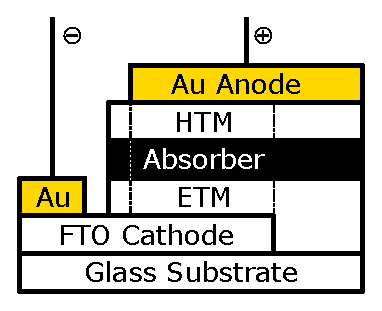
\includegraphics[width=0.4\textwidth]{bottom_top_cathode/bottom_cathode.pdf}
			\mycaption[Bottom cathode solar cell.]{The stack of a bottom cathode solar cell.
				The shapes dimensions does not relate to real thicknesses and areas.
				The dashed lines indicate the active area.}\label{fig:bottom_cathode}
		\end{SCfigure}

		\paragraph{Cathode and \gls{etm} substrate preparation}
		This process was performed in a ISO~7 clean room.
		Pre-patterned \SI{1.5 x 1.5}{\cm} \gls{fto} coated glasses were employed as substrate.
		The identification code was scratched with a diamond tip pencil.
		Initially the dust is removed with adhesive tape and rubbing with a dust free cloth.
		Then the substrates were cleaned with ultrasonication in water with Hellmanex soap, then in deionized water, and finally in isopropanol; dried rubbing with a dust free cloth and the organic residuals were removed with an UV/ozone treatment for \SI{20}{\min}.
		Dense (as opposed to mesoporous) \ch{TiO2} layer was deposited (static dispensing, \SI{80}{\ul}) from the solution described in \cpageref{precursors_tio2} by spin-coating at \SI{3000}{\rpm}, \SI{3000}{\rpm\per\s}, for \SI{60}{\s} (\SI{\approx 30}{\nm}) over the previously cleaned \gls{fto}.
		The substrates were placed in a glass Petri dish kept slightly open (this helps the removal of the burnt organic residuals and manages to reduce the entrance of dust) and inserted in a muffle oven.
		The sintering can also be performed placing the substrates on a titanium hotplate, but the amount of dust on the deposited layer is greater.
		Then the substrates were sintered at \SI{500}{\celsius} for \SI{30}{\minute} and cooled down slowly for not breaking the Petri dish.
		Subsequently the substrates were immersed in a filtered (\gls{pes}, \SI{0.22}{\um}) \SI{40}{\milli\Molar}
		\ch{TiCl4} solution in 9~\% \ch{HCl} in an oven at \SI{70}{\celsius} for \SI{20}{\min} (this process erode the titania layer, so it's important to not exceed in the duration), cleaned with water, with isopropanol and calcined as aforementioned at \SI{500}{\celsius} for \SI{30}{\min}.
		The usage of a thicker glass (\SI{2.2}{\mm}) as compared to the one used for top cathode cells (\SI{1.1}{\mm}) and the usage of \gls{fto} in place of \gls{ito} are needed for resisting the high temperature processing of the titania layer.
		Please note that \gls{fto} absorbs more in the infrared region than \gls{ito} and is more rough.

		%\paragraph{\Acr{mapi} Perovskite Two Step Fabrication}	
		% ig87

		\paragraph{\Acr{csfamapbibr} perovskite one step fabrication}

		This process was performed in a nitrogen-filled glovebox
		while constantly purging with a nitrogen flow for reducing the \gls{dmf} and \gls{dmso} vapours concentration.
		Perovskite precursor solution (see \cpageref{precursors_csfamapbibr}) was filtered (\SI{0.2}{\um}, \gls{ptfe})
		and deposited by spin-coating (\SI{80}{\ul}, static dispensing, first step \SI{1000}{\rpm}, \SI{1000}{\rpm\per\s}, \SI{10}{\s};
		second step \SI{6000}{\rpm}, \SI{1000}{\rpm\per\s}, \SI{20}{\s}; fast crystallization was induced dynamically
		dispensing \SI{50}{\ul} of chlorobenzene on the spinning substrate \SI{5}{\s} before the end of the second
		step) obtaining a \SI{500}{\nm} thick perovskite layer.
		The substrates were immediately transferred from
		the spin coater to a hot plate and annealed at \SI{100}{\celsius} for \SI{60}{\minute}.
		After removing from the hotplate, the devices were stored in a glass Petri dish for protecting from dust deposition.
		It was left partially open to avoid accumulation of vapours from solvent residuals.

		\paragraph{\Gls{htm} and cathode deposition}
		The \gls{htm} solutions (\gls{spiro}, \gls{tae1}, \gls{tae3}, or \gls{tae4}) were filtered (\SI{0.2}{\um}, \gls{ptfe}) just before usage and deposited by spin-coating in a nitrogen-filled glovebox
		onto the perovskite layer (\SI{60}{\ul}, static dispensing, \gls{spiro} at \SI{4000}{\rpm}, \SI{4000}{\rpm\per\s},
		for \SI{30}{\s}; \gls{tae1} and \gls{tae3} at \SI{2000}{\rpm}, \SI{2000}{\rpm\per\s}, for \SI{30}{\s}; \gls{tae4} at \SI{1000}{\rpm}, \SI{2000}{\rpm\per\s},
		for \SI{45}{\s}) and similar \gls{htm} thicknesses were obtained (\SI{\approx 100}{\nm}).
		\Gls{fto} contact was cleaned on two edges scratching away the \gls{htm} and perovskite materials; then the edges were further cleaned rubbing them with swabs slightly wet with \gls{dmso} (the solvent vapours can damage the perovskite layer).
		%, that's why this process is done after \gls{htm} deposition and just for what's remaining after mechanical scratching most of the material).
		Unless otherwise specified, in order to increase the
		oxidative doping of the \gls{htm} in a more or less controlled way, the devices were kept \SI{1}{\hour} in dark in a dry air chamber.
		Finally, \SI{80}{\nm} of gold was deposited by thermal evaporation in an ultra-high vacuum chamber
		(\SI{1e-9}{\bar}, MBraun) using a shadow mask leading to 4 diodes for substrate each with an active area of
		\SI{9}{\mm\squared}.
		\label{methods_bottom_end}


		\FloatBarrier
	\subsection{Handling and Preservation}

		\paragraph{Oxidative doping of \gls{htm}}
		In case of bottom cathode cells, the oxidation of the \gls{htm} has been proven to improve the \gls{pce}.
		The oxidation can be induced using dopants, for example FK 209 Co(III) TFSI salt\cite{Burschka2013} (this was not done in this thesis), or \textsl{via} oxygen exposure in dark.

		\paragraph{Degradation due to oxygen and illumination}\label{methods_degradation}
		A synergic light and oxygen contribution on the perovskite layer degradation has been reported CITATION.
		In \cref{fig:microscope_degradation} the degradation of a complete device exposed to continuous illumination for \SI{10}{\minute} and ambient air conditions is shown.
		An analogous device kept in air but without illumination did not show any degradation as observable \textsl{via} optical microscopy.
		The presence of mesoporous titania in the photographed solar cell helps the permeation of oxygen allowing the degradation to occur in every zone of the device.
		Interestingly the degradation is more prominent at metallic contacts' edges, one could speculate the reason being the electrical field being higher at smaller curvature metallic edges.
		It could also be that the ionic profile of perovskite when holes quasi Fermi level is pinned at gold workfunction makes perovskite more sensible to degradation, and this is more evident at edges due to oxygen diffusion being blocked by the gold layer.
		Even if storage in dark and dry air should not be damaging for perovskite solar cells, usually the long-term storage happens in a nitrogen-filled glovebox.


		%The oxygen can enter in direct contact with the perovskite layer due to permeability of the \gls{htm}; additionally, when a mesoporous \gls{etm} is used (e.g. titania) oxygen can diffuse rapidly through the partially infiltrated mesoporous structure. For this reason a cabinet has been modified adding of a constant dry air inlet. The gold contact was not enough for protecting the perovskite layer from degradation, as oxygen could penetrate through the mesoporous titania. 
		\begin{figure}%[!hbtp]%
			\makebox[\textwidth][c]{
				\parbox{1.1\textwidth}{
					\centering
					\begin{subfigure}[b]{0.3\textwidth}
						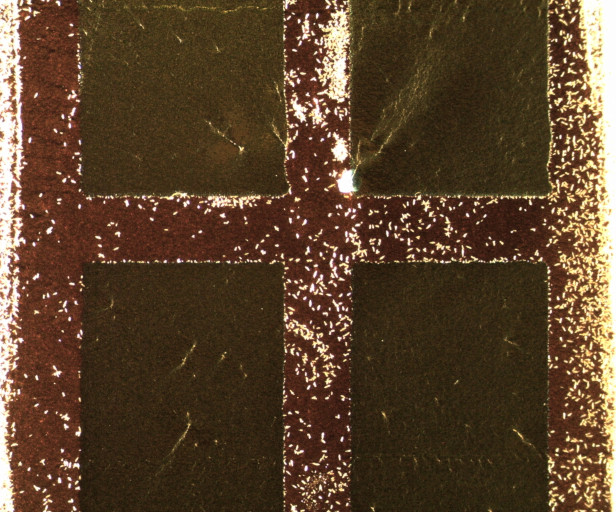
\includegraphics[width=1\textwidth]{microscope_degradation/ig93-1387-1-rescaled.jpg}
						\subcaption{Original, gold side.}\label{fig:microscope_degradation-start}
					\end{subfigure}
					\quad
					\begin{subfigure}[b]{0.3\textwidth}
						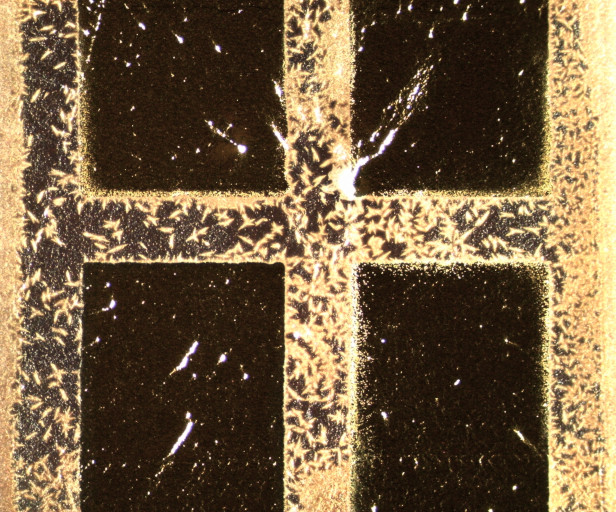
\includegraphics[width=1\textwidth]{microscope_degradation/ig93-1387-8-rescaled.jpg}
						\subcaption{\SI{10}{\minute}, gold side.}\label{fig:microscope_degradation-end_front}
					\end{subfigure}
					\quad
					%	\bigskip\newline
					%
					\begin{subfigure}[b]{0.3\textwidth}
						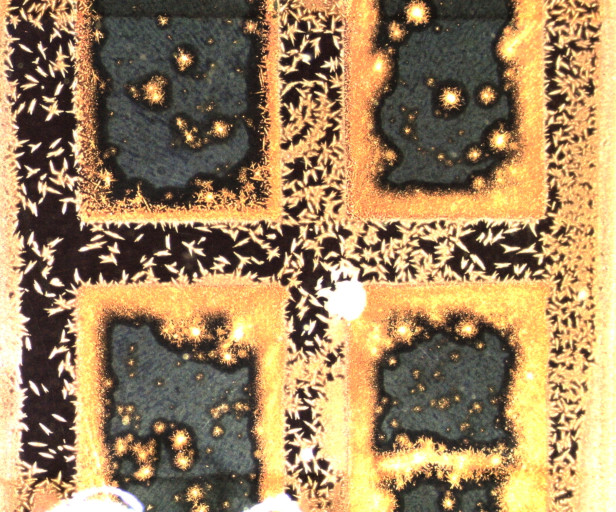
\includegraphics[width=1\textwidth]{microscope_degradation/ig93-1387-back-rescaled.jpg}
						\subcaption{\SI{10}{\minute}, glass side.}\label{fig:microscope_degradation-end_back}
					\end{subfigure}

					\mycaption[Degradation due to oxygen and illumination combination.]{A \gls{fto}\-/\ch{d-TiO2}\-/\ch{mp-TiO2}\-/\acr{csfamapbibr}\-/\gls{spiro}\-/\ch{Au} device upon \SI{10}{\minute} illumination in air.}\label{fig:microscope_degradation}
				}
			}
		\end{figure}



	\clearpage
	\stopcontents[methods]

\chapter{Characterisation Techniques: Description and Interpretation}\label{ch:characterization}
\chaptermark{Characterization Techniques}
	\epigraph{\textit{\enquote{If I made it, I think everybody can do it.}}}

	\addthumb{\thechapter}{\LARGE{\textbf{\textrm{\thechapter}}}}{white}{colorthree}


	\paragraph*{Abstract} Characterisation of perovskite solar cells is a non-trivial subject, the techniques researchers successfully employed for \gls{osc} and \gls{dssc} needs to be re-validated for this new kind of solar cells.
	The presence of ionic migration in the absorber can be a game-changer for which special care has to be taken.
	In this chapter the employed characterisation techniques are described and critically assessed.
	Taking advantage of drift\hyp{}diffusion simulations, some new hypotheses are thrown about the interpretation of the characterisation output.
	
\newpage
%Important to finish this paragraph, for example with an empty line for avoiding the following error:
% .ptc Something's wrong--perhaps a missing \item. ...rline {4.1}Introduction}{89}{section.4.1}
	\centerline{\rule[0.5ex]{0.2\linewidth}{1pt} \textbf{Table of Contents} \rule[0.5ex]{0.2\linewidth}{1pt}}
	
	\startcontents[characterization]
	\printcontents[characterization]{l}{1}{\setcounter{tocdepth}{4}}

	\centerline{\rule[0.5ex]{0.5\linewidth}{1pt}}

	\graphicspath{ {./contents_img/characterization/} }

	\newpage
	

\section{Conventions and General Remarks}

	All the characterisation on complete devices was performed keeping them in an air-tight holder filled with nitrogen.
	The electrical connection from the cell electrode to the external end of the holder was obtained using gold tips connected \textsl{via} a printed circuit board to a coaxial cable.

	\subsection{Sign Convention and Parameters Definitions}

		\paragraph{Fermi level}
		The electrons electrochemical potential, also known as Fermi level, is defined as the energy required for adding an electron in a specified position.
		Its value depends on the electrostatic potential $V_|E|$ in that position and on the internal chemical potential $\mu$ which in our case depends mainly on the concentration of electrons (not related to their electric charge, similarly to the density of a gas).
		As the Fermi level is going to be used mainly for comparisons, its zero is not going to be defined thesis-wide, instead it will be defined to a convenient reference just where needed.

		\paragraph{Cathode and anode}
		Considering a solar cell device at steady state under illumination and in open circuit conditions, its cathode is defined as the electrode where the electrons electrochemical potential $\bar\mu$ (quasi-Fermi level of electrons including the electrostatic contribution) is the highest.
		By consequence the other electrode is the anode.
		In any illumination and applied voltage case, the naming of the two physical electrodes holds to the one just defined for the illuminated device at open circuit conditions.
		% in illuminated, open circuit conditions even in conditions where the contacts' electrochemical potential is in the reversed order.

		\paragraph{Voltage}
		The voltage $V$ is a relative value indicating a difference of electrons electrochemical potential in two different physical locations.
		It can be obtained subtracting the electrons electrochemical potential at the cathode position, from the one at the anode position.
		So in the aforementioned solar cell example, the voltage is positive.
		The unit is the Volt.

		\paragraph{Electrical power}
		The electrical power $P$ is defined as positive when the device absorbs electrical energy (incoming, passive element as a resistance) and negative when it generates energy (outgoing, active element as a solar cell in working conditions).
		It can be expressed in extensive form with power (Watt) unit or in intensive form "electrical power density" with power over active area unit (Watt over square centimetre).

		\paragraph{Current and current density}
		The current $J=P/V$ is measured through an external circuit and the sign is a consequence of the voltage and electrical power definition: a current ("conventional current", flow of positively charged particles) being released from the device's anode and being received from the device's cathode is defined as negative.
		The sign convention can be understood thinking that: inside the device, somehow, a positive charge was moved from the high Fermi level contact to the low Fermi level contact, increasing its electrochemical energy, the opposite to what would happen in a resistor, whose current is always positive.
		In a solar cell device, the current (and the related electrical power) can be either positive or negative depending on the illumination and voltage conditions.
		It can be expressed in extensive form with current (Amperes) unit or in intensive form "current density" with current (Amperes) per active area (square centimetre) unit.

		\begin{SCfigure}
			\centering
			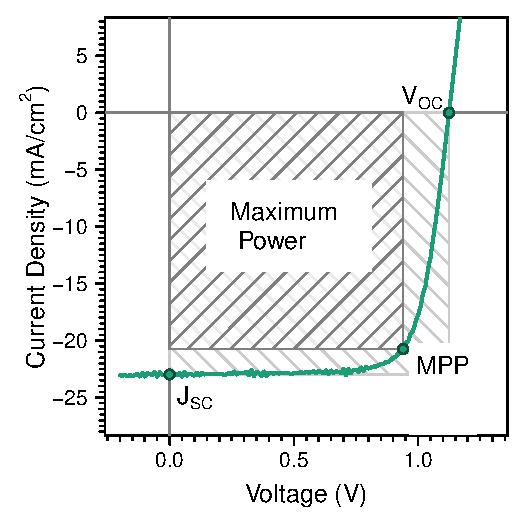
\includegraphics[width=0.5\textwidth]{iv_params/IV-revIVs.pdf}
			\mycaption[Solar cells parameters from current-voltage sweeps.]{A typical current-voltage sweep is represented.
				MPP stands for maximum power point, \gls{jsc} stands for \glsdesc{jsc}, \gls{voc} stands for \glsdesc{voc}.
				The ratio between the small and the large rectangles areas is the \gls{ff}.}\label{fig:iv_params}
		\end{SCfigure}

		\paragraph{\Glsdesc{voc}} \Gls{voc} parameter is defined as the voltage $V$ at which the current is zero while the solar cell device is illuminated at 1~sun conditions and in steady state (positive by its own definition).

		\paragraph{\Glsdesc{jsc}} \Gls{jsc} parameter is defined as the unsigned value of the current density flowing in an external circuit short circuiting (zero resistance) the solar cell device's contacts while illuminated at 1~sun and in steady state.
		It is usually reported in current (milli Amperes) over active area (square centimetre) unit.

		\paragraph{Maximum power density} The maximum power density is defined as the unsigned minimum of electrical power density which can be obtained by $P(V) = J(V) \cdot V$.
		It is usually reported using power (Watt) over active area (square centimetre) unit.

		\paragraph{\Glsdesc{pce}} \Gls{pce} parameter is defined as the maximum power density over the illuminating power density, which at 1~sun AM 1.5G is defined to \SI{100}{\mW\per\square\cm}.
		It is usually reported as a percentage.

		\paragraph{\Glsdesc{ff}} \Gls{ff} parameter is defined as the ratio between \gls{pce} and the product of \gls{voc} and \gls{jsc}.
		This parameter does not have a physical meaning, but it represents how much the series and shunt resistances affect the device efficiency.
		It can be represented either as a fraction of unity or as a percentage.

		\paragraph{Forward and reverse bias} Forward bias is a device condition where the voltage is positive, reverse bias is the case where the voltage is negative.

		\paragraph{Forward and reverse scan} In current-voltage sweeps, a scan where the voltage is increasing over time is a forward scan, while a voltage variation in the opposite direction constitutes a reverse scan.

		\paragraph{Ideality factor} An ideality factor $n_|id|$ different from 1 describes deviations from the ideal photo-diode.
		The Shockley diode equation adapted for photogeneration becomes \cite{Calado2019}:
		\begin{equation} \label{eq:photodiode}
			J(V,\phi) = J_|ph|(\phi) - J_0\left[\exp(\frac{qV}{n_|id|k_|B|T})-1\right]
		\end{equation}
		where $J_|ph|$ is the total photo\hyp{}generated current (negative sign), $J_0$ is the dark diode saturation current (the current flowing in dark when applying a reverse bias, negative sign), $q$ is the elementary charge, $k_|B|$ is the Boltzmann constant, and $T$ is the temperature.
		If recombination losses at short circuit are negligible (which can be measured either with $\jsc$ \textsl{versus} $\phi$, see \cpageref{jsc-phi}, or with \gls{tpc}, see \cpageref{characterization_tpc}), the photo\hyp{}generated current can be approximated with the short circuit current $J_|ph|(\phi) \approx \jsc(\phi)$.
		Clearly the reported equation just offers a simplified model.
		For example, it can be improved adding the contribution from the series resistance $R_|s|$ and would become:
		\begin{equation}\label{eq:series_resistance}
			J = J_|ph|(\phi) - J_0\left[\exp(\frac{q(V+JR_|s|)}{n_|id|k_|B|T})-1\right]
		\end{equation}
		The function is now an implicit one, requiring numerical solving even for obtaining $\jsc$.
		Additionally, we can include the leakage current due to the internal shunt resistance $R_|sh|$ \cite{Nelson2003}:
		\begin{equation}
			J = J_|ph|(\phi) - J_0\left[\exp(\frac{q(V+JR_|s|)}{n_|id|k_|B|T})-1\right] + \frac{V+JR_|s|}{R_|sh|}
		\end{equation}

		\paragraph{Top and bottom of devices} The point of view of the manufacturer is used for defining the physical top and bottom of a device: the bottom is the glass substrate and the top is the last deposited layer.
		This is opposite with the usage of a solar cell in the real world and with most of the solar simulators (but not all of them
		%, for example Paios from Fluxim has an illumination from below, more convenient for contacting the electrodes without a samples holder
		\cite{Fluxim}).

	\subsection{Usage of Shadowing Mask}

		\begin{SCfigure}
			\centering
			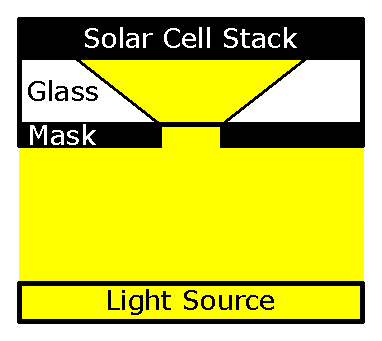
\includegraphics[width=0.35\textwidth]{shadowing_mask/shadowing_mask.pdf}
			\mycaption[Illuminated area after a shadowing mask.]{This schema is just for explaining the concept described in the text, its dimensions are not realistic.}\label{fig:shadowing_mask}
		\end{SCfigure}

		In literature is generally suggested to use a shadowing mask when measuring the solar cell devices in order to better define the illuminated area (\textsl{e.g.} in the obsolete \cite{Brinser2017} form by Nature publisher \cite{NatureResearch2017} or in \cite{Christians2015}).
		Our active area is just \SI{0.09}{\square\cm} so the mask aperture should be extremely small and its positioning troublesome.
		Additionally, the fact that the illumination reaches the mask from a wide angle (the illumination passes through spread lenses, whose size is not small compared to the lamp-cell distance) allows the light to spread through the substrate glass (\SI{2.2}{\mm} for our \gls{fto} substrates) illuminating a large area on the active layer, as represented in \cref{fig:shadowing_mask}.
		In our solar simulator a linear widening of 8~\% over \SI{2}{\mm} was estimated, this makes an illuminated area 16~\% larger than the mask aperture.
		Even if the total incident power is determined from the mask aperture, the incident intensity is not 1~sun any more, compromising the validity of the measurement.


	\subsection{Stability During the Measurement and Small/Large Perturbations}

		Most of the reported hybrid lead halide perovskite materials can show rather impressive changes in their structure on long time scales, for example due to ionic migration \cite{Calado2016}, degradation \cite{OKane2019}, and self-healing \cite{Ceratti2018}.
		This have to be taken into account for all the measurements techniques output which either takes too long time to be measured or employs large perturbations.

		\paragraph{Long lasting measurement}
		An example of the first case is the impedance spectroscopy where during the long lasting measurement various phenomena can occur, like: a slow current evolution due to perovskite well known hysteretic behaviour prior to stabilization; a degradation process changing the current; the heating of the device changing its properties.
		This slow current evolution can easily be misinterpreted for capacitive current \cite{Jacobs2018}, introduce artefacts like loops in the Nyquist plots \cite{Moia2019}, or even justify negative capacitance observations \cite{Knapp2015}.

		\paragraph{Large perturbations} \label{perturbation}
		Large perturbations regime means that the independent variable is changed by an amount large enough to cause the dependent variable to not adhere to the first term of its series expansion.
		Let's take some examples.
		%		\paragraph{Large perturbations -- \gls{tpv}}
		For example, a too intense laser pulse in \acr{tpv} could change the voltage by a less\hyp{}than\hyp{}linear amount.
		In this case, the light pulse is not only probing the recombination, but it is adding some, so a large perturbation has to be avoided.
		This effect has been reported for \gls{dssc} in \authoryear{Barnes2013}.
		%		\paragraph{Large perturbations -- \gls{trpl}}
		Last example: in the \glsdesc{trpl} a laser pulse illuminates the otherwise unilluminated absorber layer.
		If mobile ions are present, this pulse induces some extent of ionic migration to a new profile \cite{Levine2018}.
		The extent of this migration will depend on the pulse intensity and duration.
		The fact that the relaxation time of the ionic migration (\si{\ms} to seconds for the ions \cite{Jacobs2018}) is usually much larger than the laser repetition rate (\si{\ms} to \si{\us} for typical \gls{trpl} lasers \cite{EdinburghInstruments}) implies that the ionic profile variation slowly "builds up" pulse after pulse.
		As the ionic profile affects the free charges concentration, and this in turn rules the radiative recombination, the measurements of \gls{trpl} have to be done with extreme care.
		An example of hysteretic behaviour observed with \gls{trpl} can be found in \authoryear{Motti2016} and elsewhere \cite{Chen2015,Chen2017}.
		%		This should also be considered when comparing life\hyp{}times from different laser fluences \cite{Manser2014}.

\section{Current-Voltage Sweeps}

	After calibrating the light intensity in the solar simulator (see \cpageref{solarsimulator}), the devices were exposed to the illumination at open circuit for some seconds in order to have a stabilized open circuit voltage.
	Then the curves were measured with the auto-measure function of the PyPV software which measures the reverse scan and then the forward scan (see \cpageref{automeasure}).

	\paragraph{Auto-scale}\label{autoscale}
	In literature one can easily find current-voltage curves with discontinuities or "kinks" \cite{Li2016,Snaith2014,Zhang2015} like the one reported in \cref{fig:autoscale}, this is usually left unexplained.
	%	Some even lucubrate about the origin of these in perovskite solar cells.
	Disabling the auto-scale feature of the Keithley equipment the discontinuities disappear, so we can account these kinks to an hysteretic effect happening during the instrumental scale change.
	%	It is likely due to the auto-scale feature of the Keithley equipment, as disabling this, the discontinuities disappear.

	\begin{SCfigure}%[!hbtp]%
		\centering
		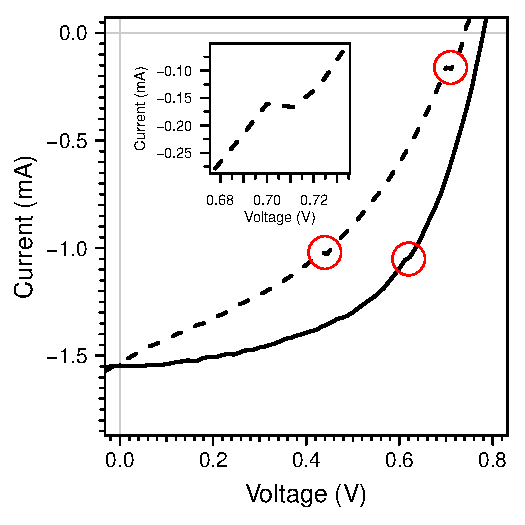
\includegraphics[width=0.5\textwidth]{autoscale/ig1-3-1-int4.pdf}
		\mycaption[Kinks in J-V sweep due to autoscale.]{A current-voltage sweep of an hysteretic perovskite solar cell with Keithley autoscale active.
			Both the forward (dashed) and the reverse (solid line) present small discontinuities around \SI{1}{\mA} and \SI{0.1}{\mA}.}\label{fig:autoscale}
	\end{SCfigure}

	\paragraph{Scan speed}
	The used sweep speed is \SI{500}{\mV\per\s}, which was arbitrarily chosen for avoiding bumps leading to currents higher than \gls{jsc}, like the one in \cref{fig:iv_ugly} (seldom reported in literature, like in figure~S3 of \cite{Du2018} or for different speeds in \cite{CorreaBaena2015,Tress2015} and simulated with drift-diffusion in \cite{Walter2018}).
	Our arbitrary choice allowed us to make fair comparisons between devices, but the absolute values should be considered as approximations.
	\begin{SCfigure}%[!hbtp]%
		\centering
		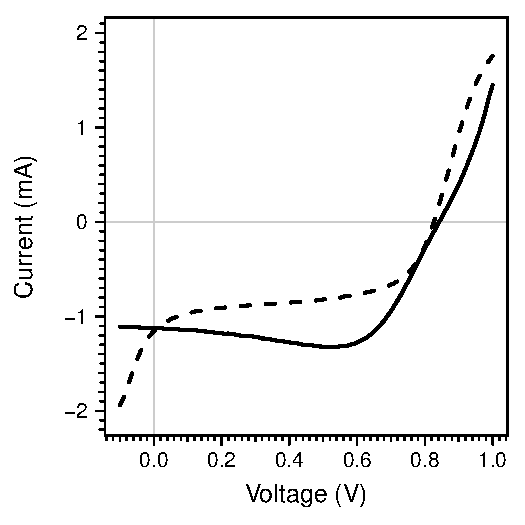
\includegraphics[width=0.5\textwidth]{iv_ugly/ig47-b32-int2-4.pdf}
		\mycaption[Hysteretic current-voltage scan.]{At the employed scan speed, the hysteresis phenomena causes the reverse (solid line) scan to reach currents higher than the \gls{jsc}.}\label{fig:iv_ugly}
	\end{SCfigure}
	We wanted to underline that due to hysteresis phenomena, no scan speed, direction, or precondition is the correct one.
	Rather, a static measurement or a \acr{mppt} should be used for obtaining a accurate and realistic result \cite{Zimmermann2016}.
	This comment regards also the so-called "hysteresis-free" perovskite solar cells, which can also present hysteretic phenomena on different time\hyp{}scales \cite{Jacobs2018,Du2018} or temperatures \cite{Bryant2015}.

	\paragraph{Noise}
	The noise often observed in current-voltage sweeps at high scan speeds in this thesis is mainly caused by oscillations in the solar simulator illumination intensity, as an example see \cref{fig:iv_params}.
	For reducing the noise impact on the \gls{jsc} and \gls{voc} parameters extraction, these values were extracted \textsl{via} a parabolic fitting.

	\paragraph{Shunt and series resistances} \label{resistances}
	The shunt and series resistances can be evaluated by the current \textsl{versus} voltage derivative of a dark current-voltage sweep.
	The former from the current values at voltages close to zero and the latter from the current at high-enough voltage.
	Perovskite solar cell hysteretic behaviour can affect this measurement.
	An alternative could be to measure the stabilised current at a few voltage points: a couple of measurements close to zero voltage is enough for estimating the shunt resistance while two points at high voltages are needed for estimating the series resistance.
	Still, the ionic profile would be different for the different applied voltages used for shunt resistance measurement, affecting the recombination barriers \cite{Moia2019,Pockett2017} so a transient measurement similar to the one proposed for the ideality factor in \cite{Calado2019} and explained in \cpageref{transient_suns_voc} should be implemented.
	In the case of series resistance, as the employed voltages are always larger than the built-in voltage, the depletion layers should be filled anyway and the transient method should not be required.

	\paragraph{Solar cells parameters extraction from sweeps}\label{characterization_hysteresis}
	For the devices studied in this thesis, the reported values of \gls{voc}, \gls{jsc}, \gls{pce} and \gls{ff} are extracted from a forward or reverse current-voltage sweep.
	This follows the tradition of solar cells reporting; but for hysteretic devices, like perovskite solar cells, a static measurement should be preferred.
	%	\paragraph{Solar cells parameters extraction from sweeps -- \gls{pce}}
	For measuring the \gls{voc} or the \gls{jsc} a static measurement is experimentally straightforward.
	Instead, for the \gls{pce}, and by consequence the \gls{ff}, a proper measurement is made difficult due to the cell evolution over time (hysteresis).
	This evolution involves a drift of the maximum power point over the time, so a static measurement is suboptimal.
	A \gls{mppt} system has to be employed in order to track the voltage evolution of this point \cite{Zimmermann2016}.
	Such a system is not trivial, as the process of localization of the maximum power point involves a varying applied voltage, which can trigger some hysteresis, some attempts to achieve a working \gls{mppt} system are described in \cpageref{software_mppt}.
	%	A proper  system needs to be bought or developed, see \cpageref{software_mppt} for thoughts about possible implementations.

	\paragraph{Stabilized or dynamic current-voltage sweeps}
	One very appealing alternative to current-voltage sweeps are the so-called "stabilized current-voltage sweeps", where at each voltage point a fixed stabilization time is waited and the stabilised current is reported \cite{Unger2014, Christoforo2015, Christians2015}.
	An improvement of this technique is named "dynamic current-voltage sweeps", here the stabilization step is of variable duration, until the current\hyp{}time derivative falls below a threshold (\textsl{e.g.}\ \SI{0.2}{\%\per\minute}) \cite{Dunbar2017,Dunbar2017a}.
	%	In this thesis, these techniques have not been used.


\section{V\textsubscript{OC} and J\textsubscript{SC} Dependence on Light Intensity}
	The solar simulator illumination intensity $\phi$ is reduced \textsl{via} neutral density filters with transmittance of 0.05, 0.12, 0.25, 0.51, 0.81 and 1 (no filter).
	The values of $\voc(\phi)$ and $\jsc(\phi)$ can be obtained from static measurements or from current-voltage sweeps.
	The static measurement of $\voc(\phi)$ at high light intensities is troublesome as it can easily damage the device.
	In this thesis, the used method is specified case by case.

	\subsection{\Glsentryshort{jsc} \textsl{versus} $\phi$}\label{jsc-phi}
		The \gls{jsc} dependency on the light intensity $\phi$ is close to linear and can be fitted with a power law:
		\begin{equation} \label{eq:jsc-phi}
			\jsc \propto \phi^\alpha
		\end{equation}
		where $\alpha$ is a free fitting parameter. Its values usually range from 0.95 to 1.

		\paragraph{Interpretation}
		An $\alpha$ value lower than 1 indicates that not all the photo\hyp{}generated charges get extracted, neither at short circuit conditions.
		This can happen due to recombination processes (non-geminate ones, for geminate recombination see \cpageref{intro_geminate}) at short circuit \cite{Credgington2011} or of other factors limiting the charge collection.

	\subsection{\Glsentryshort{voc} \textsl{versus} $\phi$ and the Ideality Factor $m$}\label{characterization_ideality}
		Setting $J=0$, which corresponds to open circuit conditions, in \cref{eq:photodiode} (without considering the series resistance correction) we can obtain a relation between \gls{jsc} and \gls{voc}:
		\begin{equation}
			\jsc(\phi) = J_0\left[\exp(\frac{q\voc (\phi)}{n_|id|k_|B|T})-1\right]
		\end{equation}
		This equation can already be used for obtaining the $n_|id|$ and $J_0$ values fitting the \gls{jsc} and \gls{voc} measured at different light intensities $\phi$ (also varying the temperature could be used for fitting the values, but it was not done during this thesis \cite{Tvingstedt2016}).
		Solving for \gls{voc} we obtain:
		\begin{equation}\voc = \frac{n_|id|k_|B|T}{q}\cdot\ln\left(\frac{\jsc}{J_0} + 1\right)\end{equation}
		Considering that the saturation current $J_0$ (current in dark under reverse bias) is much smaller than $\jsc$ for the light intensities we usually employ (down to \SI{0.05}{suns}), we can approximate to:
		\begin{equation}
			\voc \approx u_1 + \frac{n_|id|k_|B|T}{q}\cdot\ln(\jsc)
		\end{equation}
		where $u_1$ is a useless constant.
		Then if the $\alpha$ value is close enough to~1, we can use \cref{eq:jsc-phi} and further approximate for plotting against light intensity $\phi$:
		\begin{equation}\label{eq:voc_vs_phi}
			\voc (\phi) \approx u_2 + \frac{n_|id|k_|B|T}{q}\cdot\ln(\phi)
		\end{equation}
		This is the equation we commonly employ for fitting and obtaining an ideality factor value \cite{Nelson2003} as it conveniently uses a zero current measurement (\gls{voc}) so that series resistance can be completely ignored \cite{Kirchartz2012}.
		%		In some cases this latest expression is used as ideality factor definition 
		The shunt resistance will still affect the measurement \cite{Tvingstedt2017}.
		The so-obtained ideality factor $n_|id|$ is usually from 1 to 2.
		A light bias/illumination dependent ideality factor can also be measured either from a current-voltage sweeps in dark (which would be influenced by hysteretic behaviour) or from a derivative form of \cref{eq:voc_vs_phi} \cite{Calado2019}:
		\begin{equation}
			n_|id|(\phi_0) = \frac{q}{k_|B|T} \eval{\dv{V_|OC|}{\ln(\phi)}}_{\phi=\phi_0}
		\end{equation}
		%		The latter method has not been tested in this thesis as it would be affected by hysteresis.

		\begin{figure}
			\makebox[\textwidth][c]{
			\parbox{1.1\textwidth}{
			\centering
			\begin{subfigure}[t]{0.5\textwidth}
				\includegraphics[width=1\textwidth]{vapp_builtin/levels_and_ions_dark.pdf}
				\subcaption{Dark, $V=0$}\label{fig:vapp_builtin-levels_and_ions_dark}
			\end{subfigure}
			\qquad
			\begin{subfigure}[t]{0.5\textwidth}
				\includegraphics[width=1\textwidth]{vapp_builtin/levels_and_ions_dark_vapp_builtin.pdf}
				\subcaption{Dark, $V=V_|BI|$}\label{fig:vapp_builtin-levels_and_ions_dark_vapp_builtin}
			\end{subfigure}
			\mycaption[Simulated effect on the ionic profile of the application of a voltage equal to the built-in voltage.]{A $p$(\SI{200}{\nm})--$i$(\SI{500}{\nm})--$n$(\SI{200}{\nm}) homojunction device is simulated, above the energy levels are reported and below the ionic density profile is reported. In (\textbf{a}) the device is at equilibrium in dark. In (\textbf{b}) the device is in steady state in dark with an applied voltage equal to the built-in voltage $V=V_|BI| = E_|CB|^{\mathrm{ETM}} - E_|VB|^{\mathrm{HTM}}$.}\label{fig:vapp_builtin}
			}
			}
		\end{figure}

		\paragraph{Transient Suns-\gls{voc}}\label{transient_suns_voc}
		A critical analysis of these methods and the proposal of a new "Transient Suns-\gls{voc}" method can be found in \authoryear{Calado2019}.
		In their work the authors propose to precondition the device in dark at an applied voltage bias roughly equal to the built-in voltage.
		After this stabilization step the needed measurement conditions are applied (illumination is switched on and open circuit conditions are set) and the interesting quantity measured within a few milliseconds.
		The preconditioning step can increase the filling of the depletion layers in the contacts, which makes the ionic accumulation at the interface vanish through diffusion, or at least decrease.
		This is illustrated in \cref{fig:vapp_builtin} where a simulation of an homojunction device is reported.
		While the ionic profile is flat through the perovskite layer, the electronic properties of the cell can be studied using the theory from \gls{osc} \textsl{i.e.} without the influence of ionic accumulation.
		Please notice that in the real case of a heterojunction device, where the two selective contacts have different band gaps, this flattening of the ionic profile could be impossible.

		\paragraph{Interpretation} %\The \gls{voc} dependency on the light intensity $\phi$ can be fitted with a natural logarithmic dependence obtaining the ideality factor $m$. 
		\authoryear{Pockett2015} measured ideality factors of planar perovskite solar cells \textsl{via} stabilized \gls{voc} obtaining, for some cases, values as high as 5.
		Also in organic \cite{Kirchartz2011,Kirchartz2012} and silicon solar cells \cite{Breitenstein2006} ideality factors greater than 2 has been observed and explained.
		According to \authoryear{Calado2019} and \authoryear{Kirchartz2012}, the ideality factor, once obtained in the correct way, is 1 when studying most of the recombination types and 2 for mid-gap trap mediated recombination in regions where the electrons and holes concentrations are similar, $n \approx p$.

		\FloatBarrier
		\newpage
\section{Charge Extraction (\glsentryshort{ce})}

	\begin{SCfigure}
		\centering
		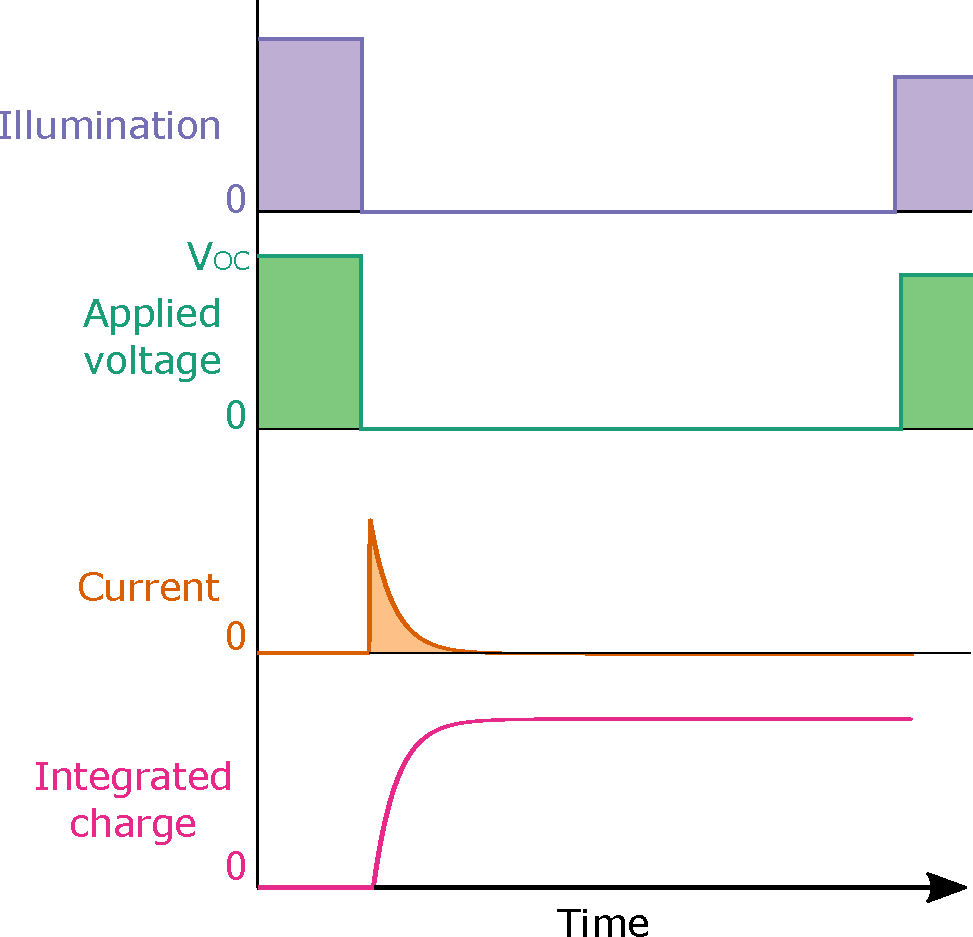
\includegraphics[width=0.6\textwidth]{ce_scheme/ce_scheme.pdf}
		\mycaption[Scheme of CE experiment.]{
			A device is illuminated in open circuit conditions, then simultaneously the illumination is switched off and the circuit is closed through a small resistance. The current flowing gets integrated to obtain the extracted charge. Then the illumination is switched on at a different intensity and the measurement is repeated.}\label{fig:ce_scheme}
	\end{SCfigure}


	\paragraph{Concept}
	The charge extraction experiment has been designed to quantify the free charges available in a device \cite{Duffy2000,Barnes2011}.
	It works \textsl{via} the sudden extraction of the free charges present in a solar cell illuminated at open circuit conditions.
	%	After stabilization of a device at a light intensity and an applied voltage (in our case always at \gls{voc}), the illumination is switched off and the electrodes of the device are short circuited.
	%	The transient current flowing through the short circuiting circuit can be measured and integrated to estimate the available charge.
	The measured charge has to be considered as a lower bound to the actually present excess charge, as part of it could recombine inside the device during the extraction time \cite{ORegan2005}.
	Performing this experiment at various light intensities, we can obtain a charge density \textsl{versus} light bias relationship.

	\paragraph{Procedure}
	The device is kept under constant illumination by a white \gls{led} at open circuit conditions until stabilization is reached.
	After stabilization, the illumination is suddenly switched off and, at the exactly same moment, the device is short circuited through a small and known resistance (\SI{50}{\ohm}).
	In the first microseconds, most of the free charge flows through the resistor generating a current and a voltage drop across it.
	An oscilloscope in parallel to this resistance measures the transient voltage.
	%This potential drop can be converted to current using the Ohm's law, which, integrated over time, gives the amount of extracted charge.
	The current flowing at any moment can be obtained from the measured voltage \textsl{via} Ohm's law: $J=V/R$ where $R$ is \SI{50}{\ohm}.
	This transient current can be integrated over time to obtain the extracted charge.
	Then the light intensity is decreased and the experiment is repeated, from 1~sun down to dark (in dark no signal should be observed).
	A single decay is measured for each illumination point, over a few tens of different illumination intensities.
	The results are plotted as charge density \textsl{versus} light bias.
	%, indeed some residual charge can usually be seen, the reason of this could be ionic profile updating or an insufficient darkness
	The equipment switching off the illumination and setting the short circuiting includes two transistors (in a home made circuit by Dr.\ Javier Pérez Hernández) and gets activated by a square voltage pulse from a pulse generator, the pulse is, at least, as long as the measurement window.
	From my experience, I recommend to use a short dark period in order to save time for the following stabilization step.
	1~sun equivalent illumination is defined as the illumination at which a silicon photodiode gives the same \gls{jsc} as under calibrated 1~sun from the solar simulator.
	The \gls{led}-solar spectral mismatch affects slightly the measurement, but in no case a \gls{pce} is reported from any \gls{led}-illuminated experiment.

	\paragraph{Noise sources} \label{ce_noise}
	The lack of complete stabilization of the device before the extraction of charge can introduce both an error in the measured \gls{voc} and in the extracted charge.
	Regarding the \gls{voc}, in perovskite solar cells it not only depends on the illumination intensity, but it also evolves slowly until the stabilization at the steady state value, so a well defined stabilization procedure is key for achieving reproducibility in \acr{ce} experiments.
	Regarding the extracted charge, the ionic profile can influence the amount of accumulated charge, as shown for two extreme cases of presence/absence of ionic charges in \cref{fig:ce_full_dd}, so a reproducible procedure for device stabilization will also improve the reproducibility of the integrated current amount.
	Additionally, the measurement equipment introduces some electronic noise whose effect can be mitigated through data post-processing.

	\begin{figure}
		\makebox[\textwidth][c]{
			\parbox{1.1\textwidth}{
				\centering
				\begin{subfigure}[t]{1\textwidth}
					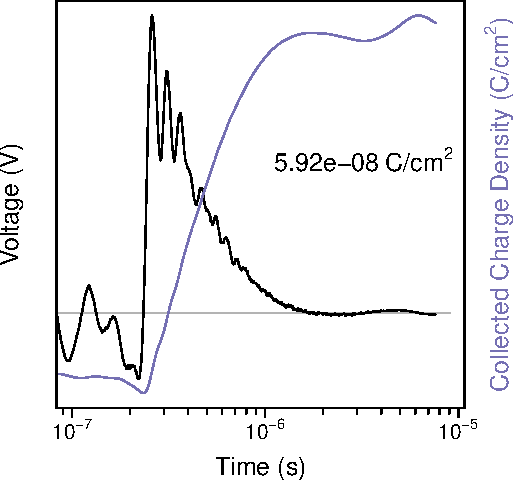
\includegraphics[width=0.45\textwidth]{{ce_noise/normal-CE_ig104-1566-4_Voc_0.911mV-crop}.pdf}
					\qquad
					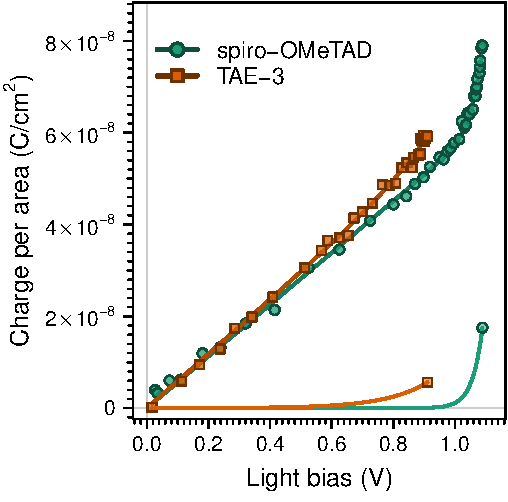
\includegraphics[width=0.35\textwidth]{ce_noise/normal-spiro_vs_TAEs-CEs-crop.pdf}
					\subcaption{Direct integration of raw data}\label{fig:ce_noise-normal}
				\end{subfigure}
				\bigskip

				\begin{subfigure}[t]{1\textwidth}
					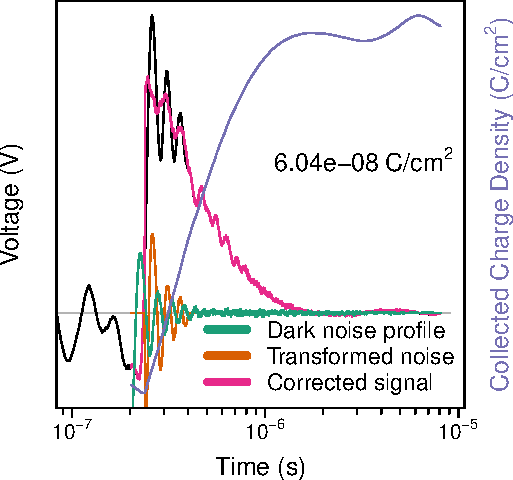
\includegraphics[width=0.45\textwidth]{{ce_noise/subtractDark-CE_ig104-1566-4_Voc_0.911mV-crop}.pdf}
					\qquad
					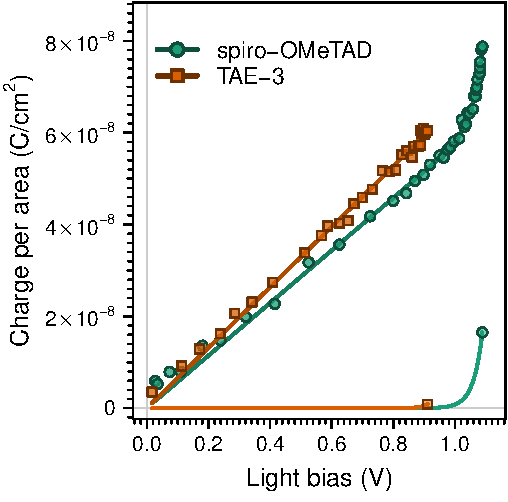
\includegraphics[width=0.35\textwidth]{ce_noise/subtractDark-spiro_vs_TAEs-CEs-crop.pdf}
					\subcaption{Subtraction of transformed noise profile}\label{fig:ce_noise-subtractDark}
				\end{subfigure}
				\bigskip

				\begin{subfigure}[t]{1\textwidth}
					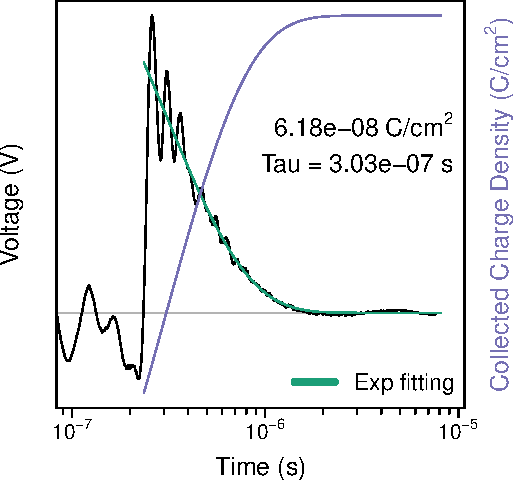
\includegraphics[width=0.45\textwidth]{{ce_noise/integrateExp-CE_ig104-1566-4_Voc_0.911mV-crop}.pdf}
					\qquad
					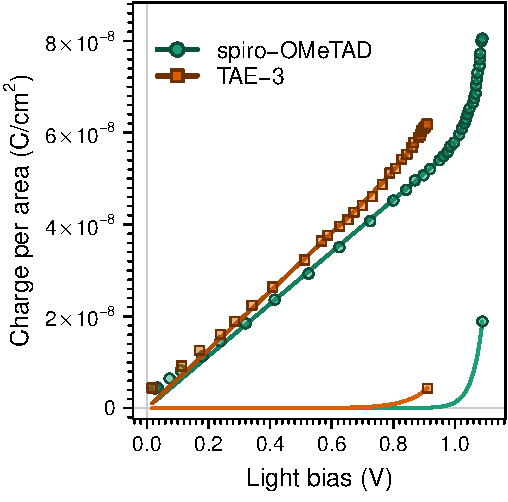
\includegraphics[width=0.35\textwidth]{ce_noise/integrateExp-spiro_vs_TAEs-CEs-crop.pdf}
					\subcaption{Integration of an exponential fitting}\label{fig:ce_noise-integrateExp}
				\end{subfigure}

				\mycaption[Strategies for reducing the instrumental noise in a single \glsentryshort{ce} integration.]{
					On the left, single \gls{ce} decays from a \gls{fto}\-/\ch{d-TiO2}\-/\acr{csfamapbibr}\-/\gls{tae3}\-/Au device \cite{Gelmetti2019} is integrated without noise reduction in (\textbf{a}), adapting the noise profile from the dark measurement and subtracting it in (\textbf{b}), or fitting the decay and integrating the fit in (\textbf{c}).
					On the right, the charge \textsl{versus} voltage trends obtained applying the respective noise reduction methods.}\label{fig:ce_noise}
			}
		}
	\end{figure}

	\paragraph{Reduction of instrumental noise}\label{r_ce_noise}
	Most of the observed short\hyp{}time noise (\SI{< 5E-7}{\s}) observable in \cref{fig:ce_noise-normal} is related to the opening and closing of the transistor switches included in the home\hyp{}made circuit.
	The characteristic frequencies of the observed noise are not small compared to the measurement window, so its time\hyp{}integral does not necessarily sum to zero.
	In order to reduce its impact, various approaches have been tested and here described.
	The noise can be ignored in some cases, but it's a problem if the charge \textsl{versus} light bias (\gls{voc} generated at a given illumination intensity) profile, reported on the right hand column of \cref{fig:ce_noise}, has to be studied in detail, as in \cref{ch:tae}.
	In the mentioned case, just the exponential part of its linear plus exponential behaviour, reported in the bottom of each right hand figure, was of interest and it is evident that the employed noise\hyp{}reduction method influences it heavily.

	\paragraph{Reduction of instrumental noise -- subtraction of dark noise}
	Annoyingly, the noise profile is characteristic of the cell and of the circuitry, so a simple average over many decays does not help in cancelling it.
	Based on this consideration, I tried to subtract a pure noise profile as obtained from a dark measurement (without any light bias).
	The operation was made more difficult by the slight variations of the noise profile with the light bias.
	A data\hyp{}to\hyp{}morphed\hyp{}noise fit was implemented where the $f(t)$ noise profile was transformed with: $t'= u_3 + u_4 \cdot t + u_5 \cdot t^2$ and $f'(t') = u_6 \cdot f(t') + u_7 \cdot t' \cdot f(t') + u_8 \cdot e^{-t'/u_9}$ where $u_{3-9}$ are constrained fit variables.
	Then $u_6$ was set to zero and the resulting profile was subtracted from the data and the result integrated.
	As can be seen in \cref{fig:ce_noise-subtractDark}, this technique is working for most of the cases but it can fail if the noise profile changes in a more complex fashion.

	\paragraph{Reduction of instrumental noise -- integration of a fitting}
	Finally the decays were fitted with a bi\hyp{}exponential formula (sum of two exponential) or, if the bi\hyp{}exponential fitting was not converging, by a simple exponential and the integral of this fit was used.
	In both cases a robust fitting routine was employed \cite{Maechler2018}.

	\paragraph{Specific limitations for perovskite solar cells} \label{ce_limitations_perovskite}
	When measuring the \gls{ce} of a perovskite solar cell, additionally to the aforementioned limitations, one should also consider that the ionic profile update (from $V=\voc$ to $V=0$) causes a displacement current, as described in \cpageref{intro_displacement_current}.
	A simulation with DrIFtFUSION is reported for an homojunction device in \cref{fig:ce_single_dd}, it can be seen that with ionic mobile defects in \cref{fig:ce_single_dd-ions_zoom} a very weak but long lasting current appears and gives a relevant contribution to the integrated charge.
	This will happen on very large time scales and it will not affect the short measurements used for the free charges estimation, so it is rarely reported \cite{ORegan2015b}.
	The charge measured in the external circuit due to the ionic displacement current could be underestimated as the free charges rearrangements can also occur through the perovskite layer rather than through the external circuit.

	INSERT FIGURE OF CONDUCTION BAND VARIATION DURING CHARGE EXTRACTION AT SHORT AND LONG TIMES HERE; WITH CHARGES REPRESENTATION

	\begin{figure}
		\makebox[\textwidth][c]{
			\parbox{1.1\textwidth}{
				\centering
				\begin{subfigure}[t]{0.5\textwidth}
					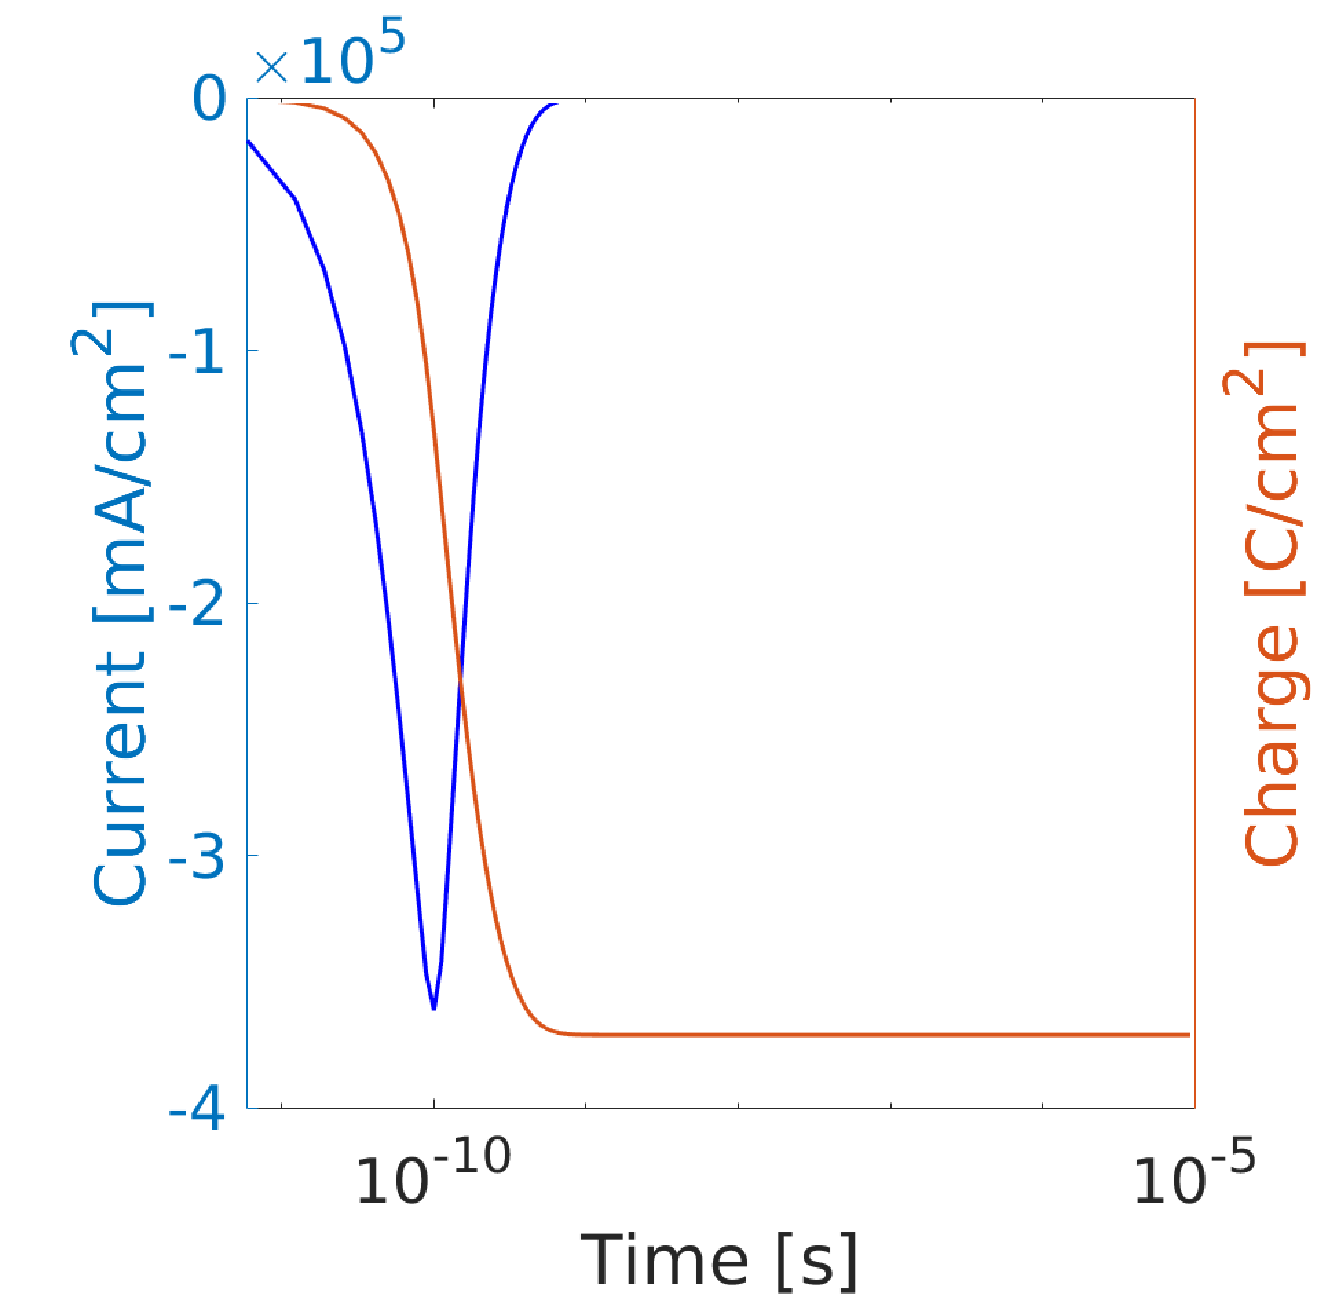
\includegraphics[width=1\textwidth]{ce_single_dd/ce_single_dd-noions.pdf}
					\subcaption{Without mobile ions}\label{fig:ce_single_dd-noions}
				\end{subfigure}
				\bigskip

				\begin{subfigure}[t]{0.5\textwidth}
					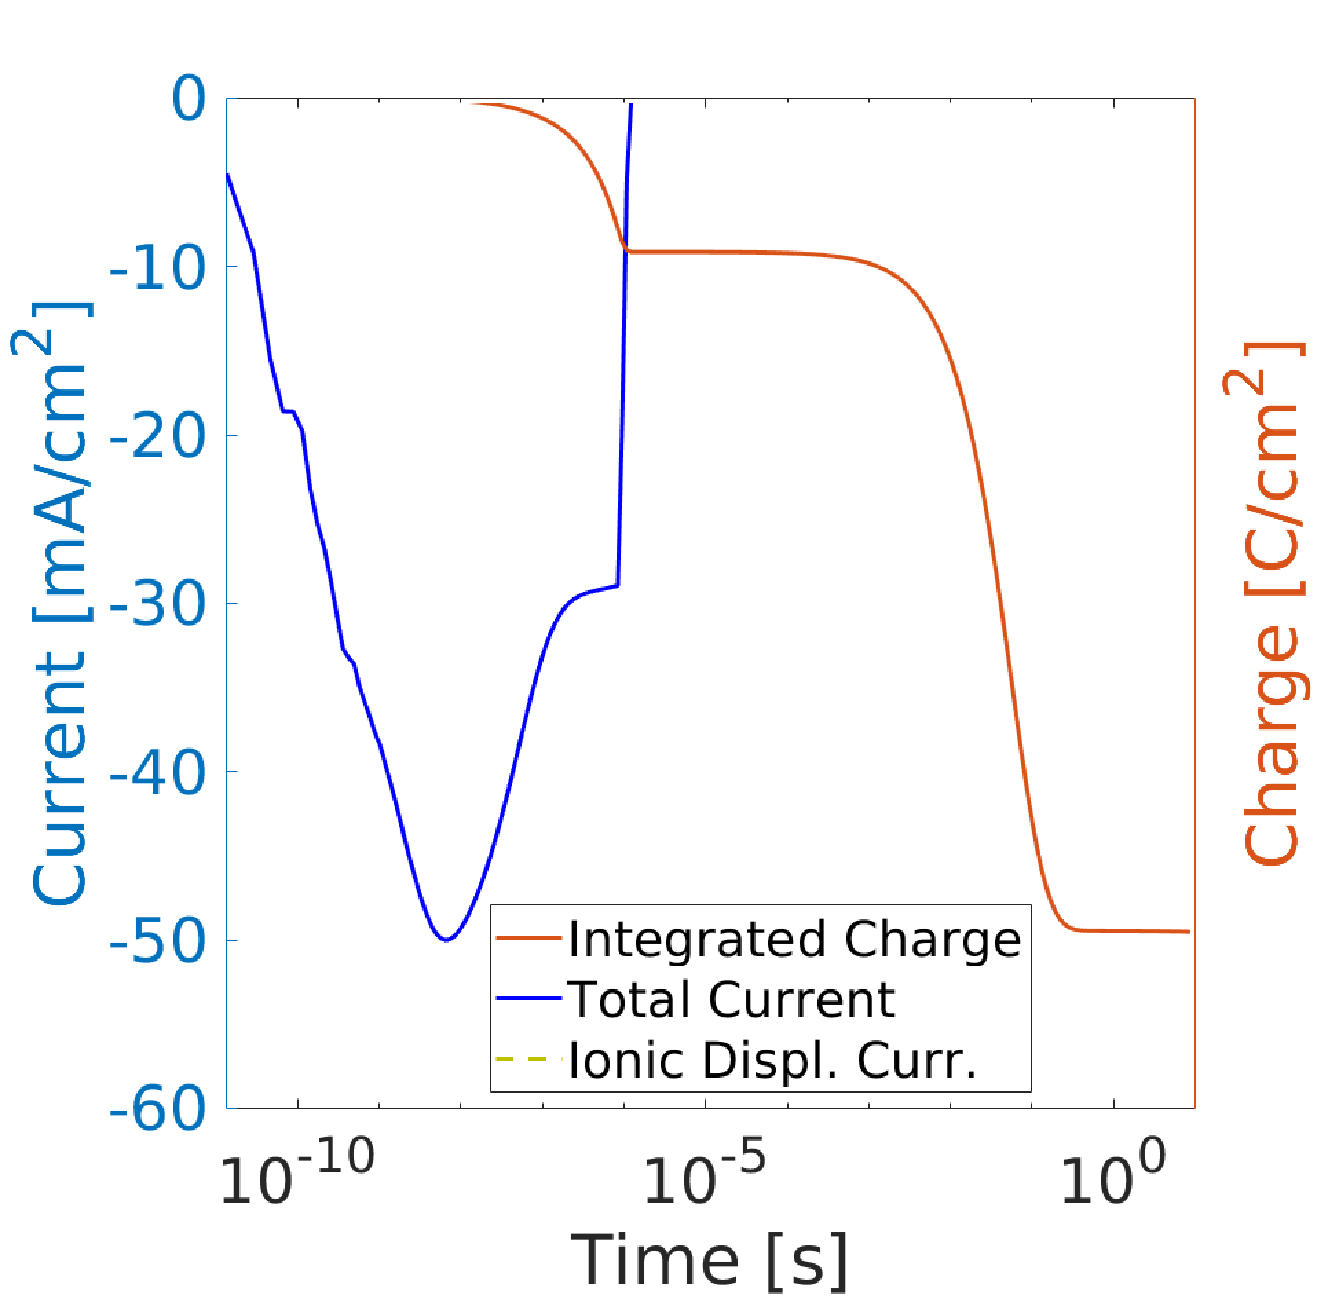
\includegraphics[width=1\textwidth]{ce_single_dd/ce_single_dd-ions.pdf}
					\subcaption{With mobile ions}\label{fig:ce_single_dd-ions}
				\end{subfigure}
				\qquad
				\begin{subfigure}[t]{0.5\textwidth}
					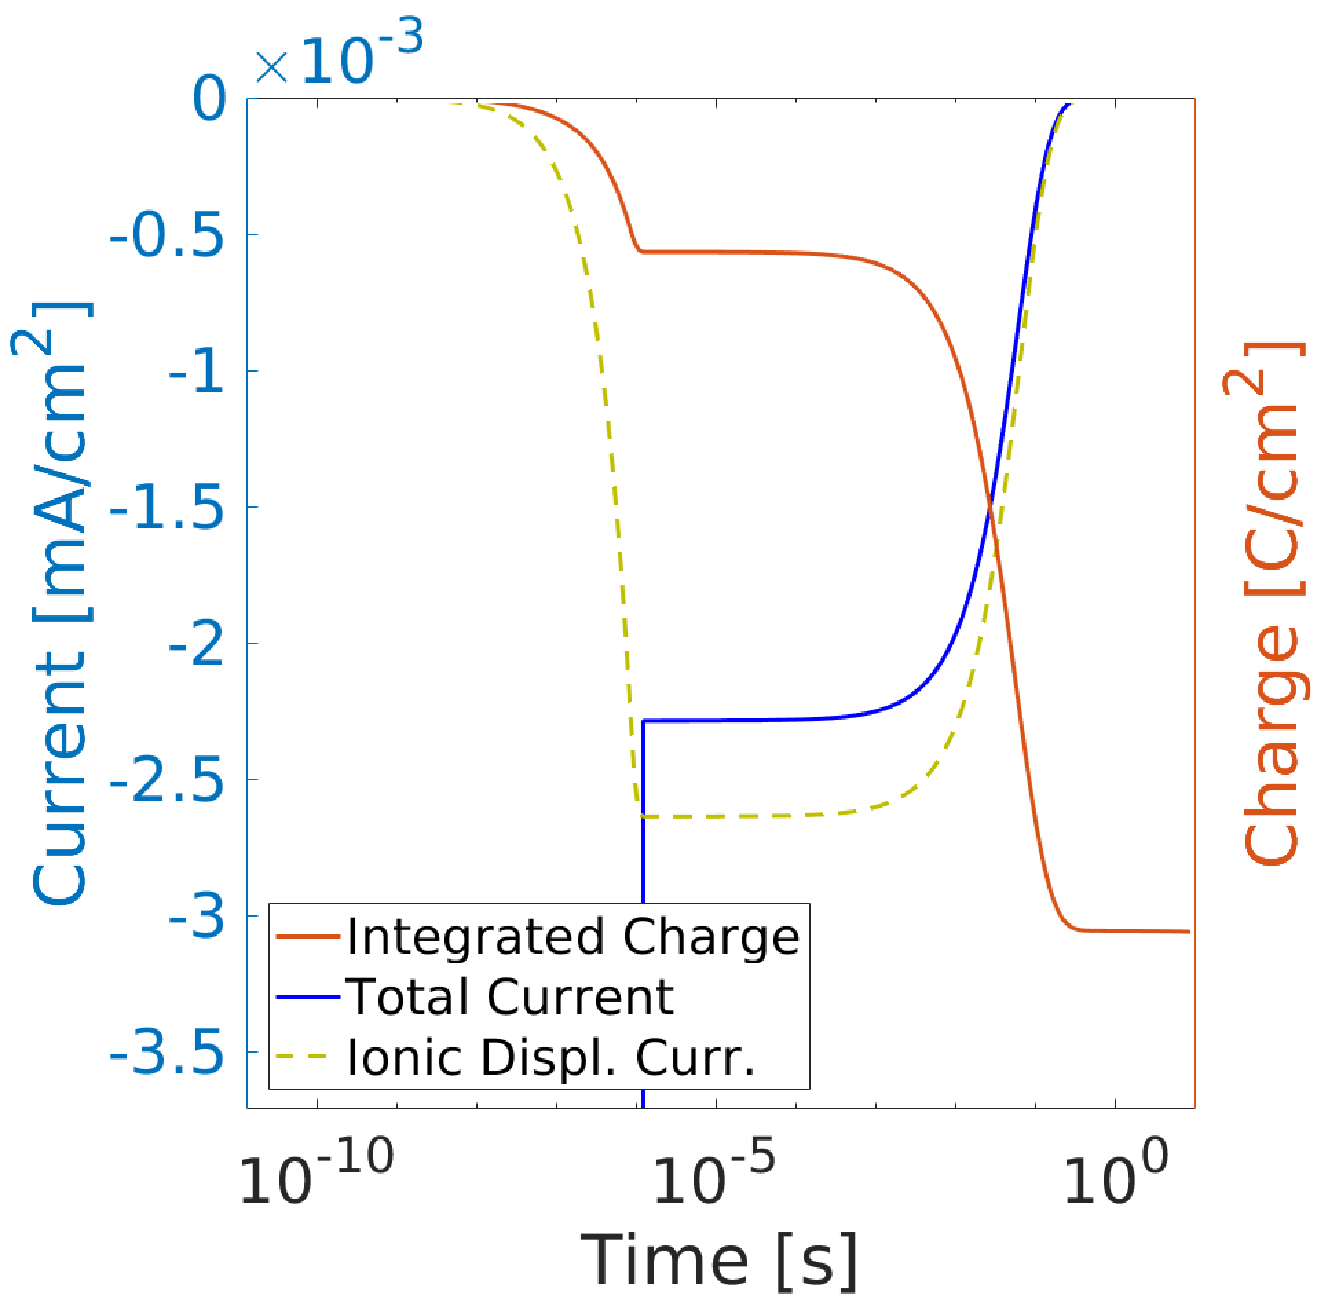
\includegraphics[width=1\textwidth]{ce_single_dd/ce_single_dd-ions_zoom.pdf}
					\subcaption{With mobile ions, magnified current density axis}\label{fig:ce_single_dd-ions_zoom}
				\end{subfigure}

				\mycaption[Simulation of a CE without or with mobile ions.]{
					The current \textsl{versus} time profile of a \acr{ce} simulated experiment is shown on the left axis just for the 1~sun illumination intensity.
					On the right axis the cumulative integration of the extracted charge.
					Clearly, the extraction is unrealistically quick as the resistance included in a real \acr{ce} experiment was not included in the simulation.
					In (\textbf{a}) the measurement of a device without mobile ions is shown, we can observe just one current peak contributing to the integrated charge; in (\textbf{b}) the presence of the mobile ions introduces a long\hyp{}times contribution to the extracted charge, the current causing this is very weak and long lasting, it can be better observed in the magnification in (\textbf{c}).}\label{fig:ce_single_dd}
			}
		}
	\end{figure}


	\subsection{Interpretation of CE Single Decays}

		\paragraph{Charge extracted}
		The integrated charge is assumed to include the excess free charges in the valence and conduction bands.
		With \emph{excess} we refer to the difference between the charge concentration in the conditions of interest and the stabilized dark condition.
		For a non perfectly crystalline material, localized shallow traps constituted by the tails of the valence and conduction bands density of states inside of the so\hyp{}called mobility gap \cite{Pieters2009} are not negligible and should also contribute to the extracted charge amount \cite{Kirchartz2012,Du2018}.
		On the contrary, charges trapped in deep traps contributing to SRH trap mediated recombination, with energies far from the band edges, should not be possible to extract in a \acr{ce} experiment.

		\paragraph{\Acr{ce} time constant}\label{ce_time}
		The free charges extraction time is related to the RC time of the \SI{50}{\ohm} resistor and the capacitance of the solar cell device.
		We can see in \cref{fig:chargeExtraction_RCtime} a weak covariance (Pearson correlation coefficient of 0.3) between the RC time obtained extrapolating the dark capacitance from \acr{dc} (which is the geometric capacitance) and the extraction time (as obtained by an exponential fitting to a single \acr{ce} current decay) at low light intensity (enough for having a signal but far from 1~sun light intensity).
		At higher light intensities, the correlation is weaker as the capacitance is less defined as the cell is in a transition between illuminated (high capacitance) and dark (low capacitance) status.
		Anyway, the extraction time does not change much between low light intensity and 1~sun with an increase from \SIrange{1.1}{2.4}{times} (first and third quartile).
		More discussion on this topic can be found on \authoryear{Montcada2018}.

		\begin{SCfigure}%[!hbtp]%
			\centering
			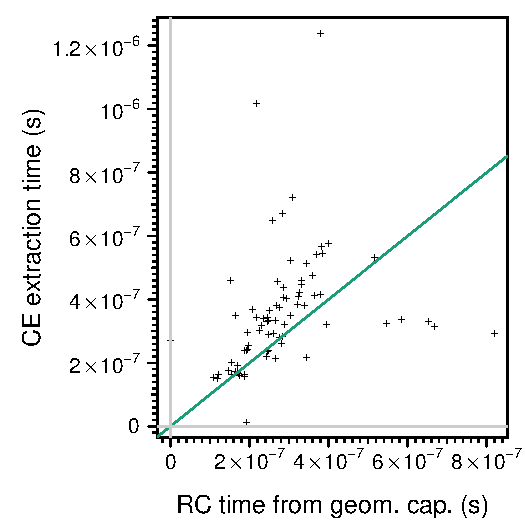
\includegraphics[width=0.45\textwidth]{chargeExtraction_RCtime/CEaBitOfSunExpTime_vs_RCdarkTime.pdf}
			\mycaption[Charge extraction time is related to a RC time.]{
				Covariance of \acr{ce} extraction time at low light intensity \textsl{versus} the expected time from geometric capacitance (as obtained from dark \acr{dc}).
				Each point is a different device for a total of 78 devices, many different structures studied during my PhD are represented.
				The green line indicates the 1 to 1 relationship.}\label{fig:chargeExtraction_RCtime}
		\end{SCfigure}

		\paragraph{\Acr{ce} time constant and \acr{tpv} time constant -- Corrections}
		During this time, and depending on its location in the device stack, some free charges can recombine.
		One could argue that a \acr{ce} measurement is valid only if the extraction is faster than the recombination time as measured via \acr{tpv} \cite{Ryan2017a} or that the extracted charge should be corrected considering the recombination \cite{Credgington2011,Credgington2014}.
		Considering the charges accumulated in the depletion layers in the selective contacts, these will flow to the electrodes without crossing the perovskite/selective contacts interfaces, where has been reported that most of the recombination occurs \cite{Barnea-Nehoshtan2014,Stolterfoht2018a,Stolterfoht2018}.
		So this part of the extracted charge, distinguishable as the linear part of the charge \textsl{versus} voltage plot, as represented on the right column of \cref{fig:ce_noise} should not be corrected.
		Instead, regarding the charge accumulating in the perovskite layer, which we assume can be assigned to a chemical capacitance and can be recognized as the exponential part on the right column of \cref{fig:ce_noise}, it may be that a correction \cite{Shuttle2008a,Shuttle2008b} is needed, but this has not be done in this thesis.

		\paragraph{\Acr{ce} time constant and \acr{tpv} time constant -- Correlation?}
		Some covariance (Pearson correlation coefficient of~0.4) can be observed in \cref{fig:ce_1sun_time_vs_tpv_1sun_time} between the \acr{ce} and the \acr{tpv} time constants at 1 sun illumination.
		This is unexpected and weird as the two times change with very different trends with light bias (when changing the preconditioning light intensity, \gls{ce} extraction time changes just slightly while \gls{tpv} decay time varies over various orders of magnitude).
		In case a stronger proof of correlation is found, this could indicate that both processes, even if not of the same nature, are limited by the same diffusion process, for example the migration of free charges from all the absorber to the absorber/contacts interfaces.

		\begin{SCfigure}%[!hbtp]%
			\centering
			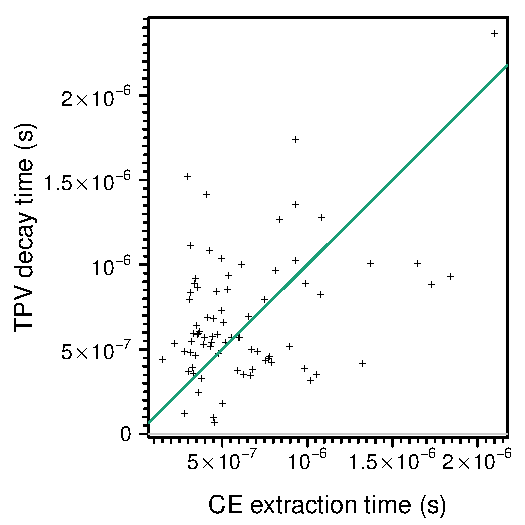
\includegraphics[width=0.45\textwidth]{ce_1sun_time_vs_tpv_1sun_time/ce_1sun_time_vs_tpv_1sun_time.pdf}
			\mycaption[Comparison between \glsentryshort{ce} and \glsentryshort{tpv} exponential decay times.]{
				Covariance of \acr{ce} extraction time at 1~sun light intensity \textsl{versus} the \gls{tpv} mono\hyp{}exponential decay time at 1~sun light intensity.
				Each point is a different device for a total of 79 devices, including many different structures.
				The green line indicates the 1 to 1 relationship.}\label{fig:ce_1sun_time_vs_tpv_1sun_time}
		\end{SCfigure}

	\subsection{Interpretation of CE \textsl{versus} Light Bias Without Mobile Ions}

		\paragraph{Exponential part and chemical capacitance in \gls{osc}}\label{ce_exp_osc}
		In \gls{osc} literature the charge \textsl{versus} light bias voltage trend is described simply as the exponential shape which describes a Maxwell\hyp{}Boltzmann distribution for a two levels scenario.
		In a few publications, the shape if fitted to an error function \cite{Ajuria2011}.
		For a common solar cell working conditions, the Maxwell\hyp{}Boltzmann classical particles approximation should be valid as the distance between Fermi level energy and the band edges is expected to be always much bigger than $k_|B|T$.
		This could be false for high applied voltages, where Fermi\hyp{}Dirac distribution for fermions should be used.
		Thus, the expression for the conduction band electronic density $n$ obtained from the mentioned distribution is:
		\begin{equation}
			n(V) = n_|DOS| \exp(\frac{qV - E_|g|}{k_|B|T}) = n_|eq| \exp(\frac{qV}{k_|B|T})
		\end{equation}
		where $n_|DOS|$ is the density of states which can be occupied by free charges, $E_|g|$ is the material band gap, and $n_|eq|=n_|DOS|\exp[-E_|g|/(k_|B|T)]$ prefactor is the equilibrium carrier concentration from a Boltzmann distribution of a two levels system. %just a pre\hyp{}factor with no direct physical interpretation.
		As the \acr{ce} can just extract the excess charge $n_|CE|$, what we can measure is:
		\begin{equation}
			n_|CE|(V) = n(V)-n(0) = n_|eq| \cdot \left[\exp(\frac{qV}{k_|B|T})-1\right]
		\end{equation}
		now the expression of $n_|CE|$ evaluated at zero voltage gives zero extra charge as expected.
		In some cases an ideality factor $m$ is introduced \cite{Kirchartz2012}, which can help to account for the shape of the density of states of the conduction band, so the expression can be found as:
		\begin{equation}\label{eq:ce_osc}
			n_|CE| = n_|eq| \cdot \left[\exp(\frac{qV}{mk_|B|T})-1\right]
		\end{equation}
		For perovskite solar cells, an alternative interpretation can be found indicating that the exponential trend reflects the extraction from exponential subgap states, \textsl{i.e.} shallow traps \cite{Du2018}.
		This can be used for explaining values of $m$ greater than 2, which would be indicative of the exponential tail width as shown for \gls{osc} by \authoryear{Kirchartz2012}.
		Moreover, in \gls{osc} has been shown that an inhomogeneous carriers concentration profile through the device thickness, likely to happen in thin films, would also cause high $m$ values \cite{Kirchartz2012} especially for low doping levels resulting in drift\hyp{}driven solar cells \cite{Deledalle2015,Deledalle2014}.


		\begin{figure}
			\makebox[\textwidth][c]{
				\parbox{1.1\textwidth}{
					\centering
					\begin{subfigure}[t]{0.5\textwidth}
						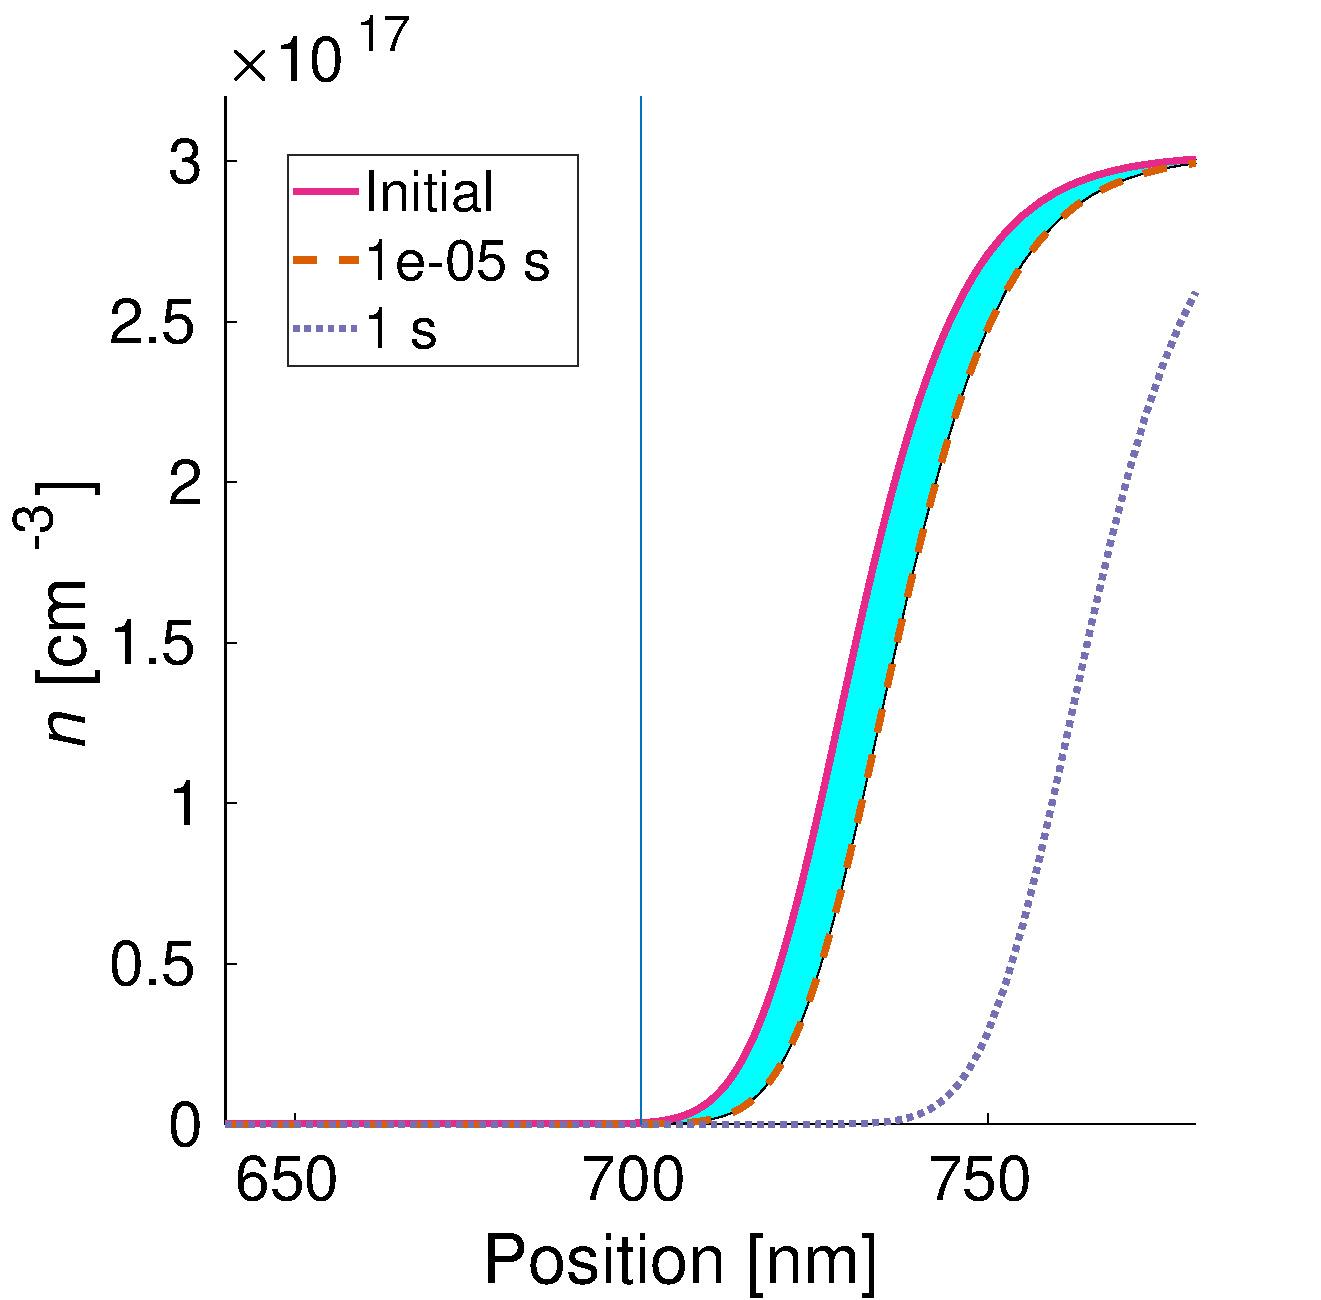
\includegraphics[width=1\textwidth]{ce_single_dd_charge/ce_ions_1sun.pdf}
						\subcaption{1 sun}\label{fig:ce_single_dd_charge-1sun}
					\end{subfigure}
					\qquad
					\begin{subfigure}[t]{0.5\textwidth}
						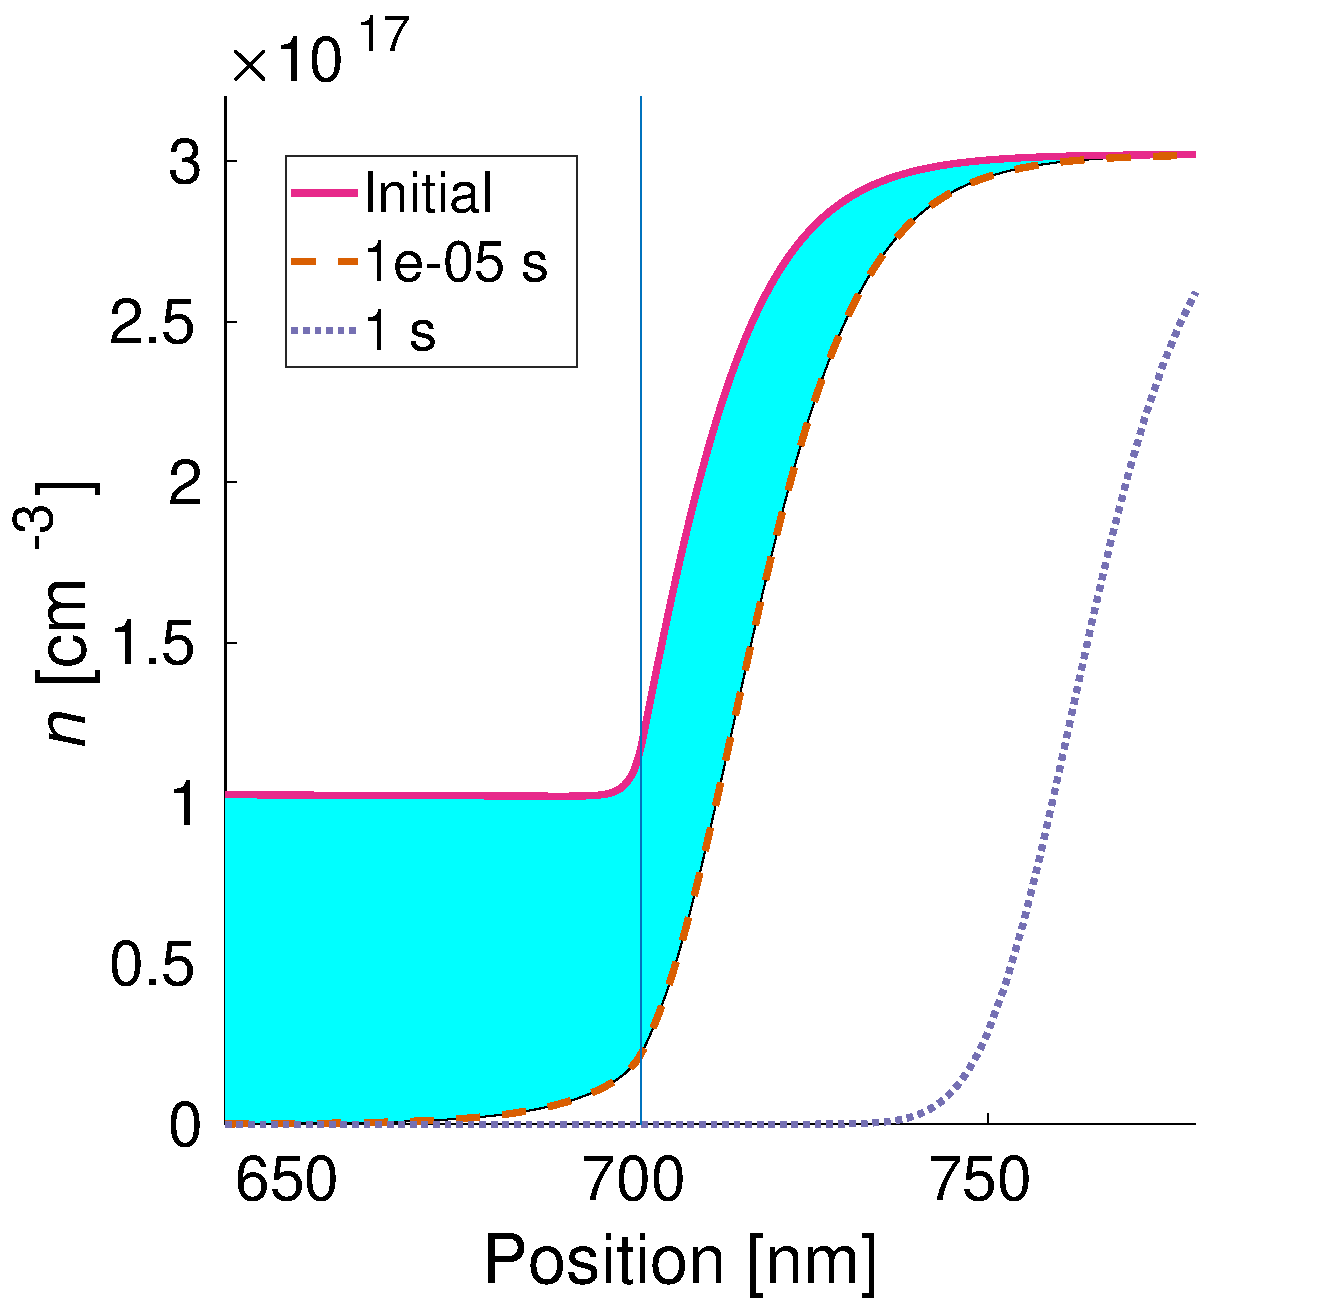
\includegraphics[width=1\textwidth]{ce_single_dd_charge/ce_ions_1000suns.pdf}
						\subcaption{1000 suns}\label{fig:ce_single_dd_charge-1000suns}
					\end{subfigure}

					\mycaption[Simulated electron density profile during a CE experiment.]{
						The electron density profile of a homojunction cell with mobile ions is plotted at the interface between perovskite (position \SI{< 700}{\nm}) and \gls{etm} (position \SI{> 700}{\nm}) at different times during a \acr{ce} experiment.
						The green solid line represent the situation as stabilized at open circuit conditions, before the \acr{ce} experiment. Corresponding energy levels for (\textbf{a}) in \cref{fig:ce_single_dd_levels-1sun} and for (\textbf{b}) in \cref{fig:ce_single_dd_levels-1000suns}.
						The dashed orange line represent the profile at short times, after the extraction of the free charges but before the reorganization of the mobile ions.
						The light blue area represents the extra charge extracted during a typical \acr{ce} experiment.
						In (\textbf{a}) the device is stabilized at 1 sun light intensity before performing the charge extraction, in this case most of the extra charge is accumulated in the contacts.
						In (\textbf{b}) the device is stabilized at 1000 suns, in which case the charge is mainly accumulated in the perovskite layer.
						The dotted violet line is the final electronic profile, at long times after the mobile ions migration, which is identical for (\textbf{a}) and (\textbf{b}) cases. Corresponding energy levels in \cref{fig:ce_single_dd_levels-dark}.
					}\label{fig:ce_single_dd_charge}
				}
			}
		\end{figure}

		\paragraph{Linear part and geometric capacitance}\label{geometric_capacitance}
		With the introduction of selective contacts, a linear contribution starts to grow in importance summing up to the exponential part.
		It has been observed both in \gls{osc} \cite{Ryan2017a,Credgington2014,Credgington2012} and in perovskite solar cells \cite{Gelmetti2017,Wheeler2017,Du2018}.
		This linear trend accounts for the accumulation in the selective contacts' depletion layers and in the electrodes, in a parallel plate capacitor fashion: $n = C_|g| \cdot V = \frac{\epsilon_0 \epsilon_|r| A}{d} \cdot V$ where $C_|g|$ is the geometric capacitance, $A$ is the active area, $d$ is the thickness of the dielectric, $\epsilon_0$ is the electric constant, and $\epsilon_|r|$ is the relative permittivity.
		This carriers accumulation in the contacts can be visualized with the simulation reported in \cref{fig:ce_single_dd_charge-1sun}.
		Extending \cref{eq:ce_osc}, the complete equation becomes:
		\begin{equation}\label{eq:ce_full}
			n_|CE| = C_|g| \cdot V + n_|eq| \cdot \left[\exp(\frac{qV}{mk_|B|T}) - 1\right]
		\end{equation}

		\paragraph{Geometric capacitance voltage dependency}
		More exactly, $d$ is the distance between the regions where the opposed charges are getting accumulated, which is the space charge layers (usually depletion layers) in the contacts.
		So this value can be somewhat wider than just the distance separating the two perovskite/contacts interfaces.
		By consequence, $\epsilon_|r|$ should be considered as a thickness\hyp{}weighted mean of the relative permittivities of each material between the two accumulation zones.
		Moreover, as the depletion layers fill up they widen and shrink, so this capacitance can vary as happens for the junction capacitance (\textsl{i.e.} transition capacitance) of a $p$-$n$ junction.
		A voltage dependent geometric capacitance can be obtained from dark \acr{ce} measurements applying reverse voltage biases \cite{Kiermasch2018} or \textsl{via} impedance spectroscopy in dark with a constant voltage bias \cite{Brus2016,Pockett2015}.
		While this dependency cannot be ignored in silicon solar cells or in \gls{osc}, where the $n$ and the $p$-type materials are in close contact, it is likely negligible in perovskite solar cells as the change of depletion layers thickness (Debye length), happening in the contacts, is negligible when summed to the perovskite layer thickness.

		\paragraph{Energy levels point of view}\label{ce_energy_levels}
		As we mentioned, the linear trend is related to the accumulation in the contacts depletion layers (or, generically, space charge layers), this can be seen from the decrease of the perovskite\hyp{}contacts conduction band offset between \cref{fig:ce_single_dd_levels-dark,,fig:ce_single_dd_levels-1sun}.
		Increasing the light illumination at open circuit conditions, the quasi\hyp{}Fermi levels splitting approaches the built\hyp{}in voltage represented by the contacts' band edges: $V_|BI| = E_|CB|^{\mathrm{ETM}} - E_|VB|^{\mathrm{HTM}}$.
		This means the depletion layers are close to saturation, like in \cref{fig:ce_single_dd_levels-1000suns} where \SI{1000}{suns} illumination was simulated, and the charge accumulates in the perovskite layer, as shown in \cref{fig:ce_single_dd_charge-1000suns}, and the exponential trend gains importance.

		\begin{figure}
			\makebox[\textwidth][c]{
				\parbox{1.1\textwidth}{
					\centering
					\begin{subfigure}[t]{0.3\textwidth}
						\includegraphics[width=1\textwidth]{ce_single_dd_levels/ce_ions_dark_levels.pdf}
						\subcaption{dark}\label{fig:ce_single_dd_levels-dark}
					\end{subfigure}
					\qquad
					\begin{subfigure}[t]{0.3\textwidth}
						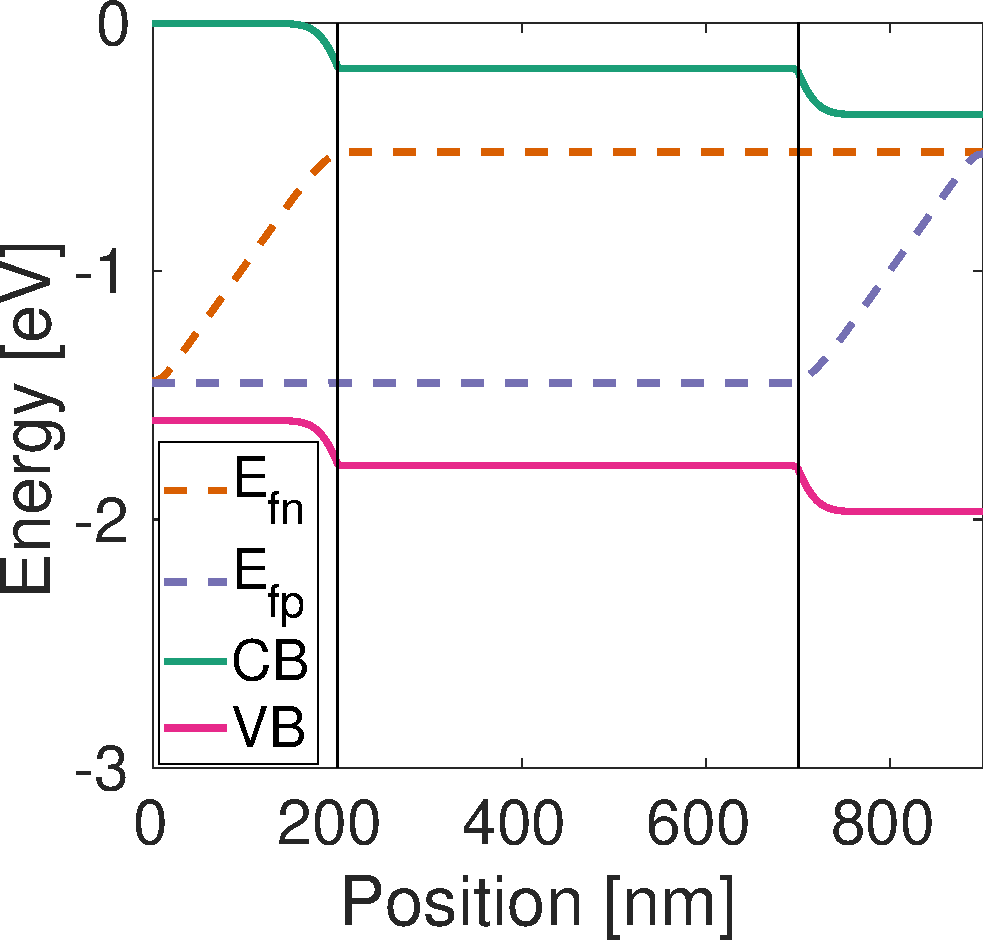
\includegraphics[width=1\textwidth]{ce_single_dd_levels/ce_ions_1sun_levels.pdf}
						\subcaption{1 sun, OC}\label{fig:ce_single_dd_levels-1sun}
					\end{subfigure}
					\qquad
					\begin{subfigure}[t]{0.3\textwidth}
						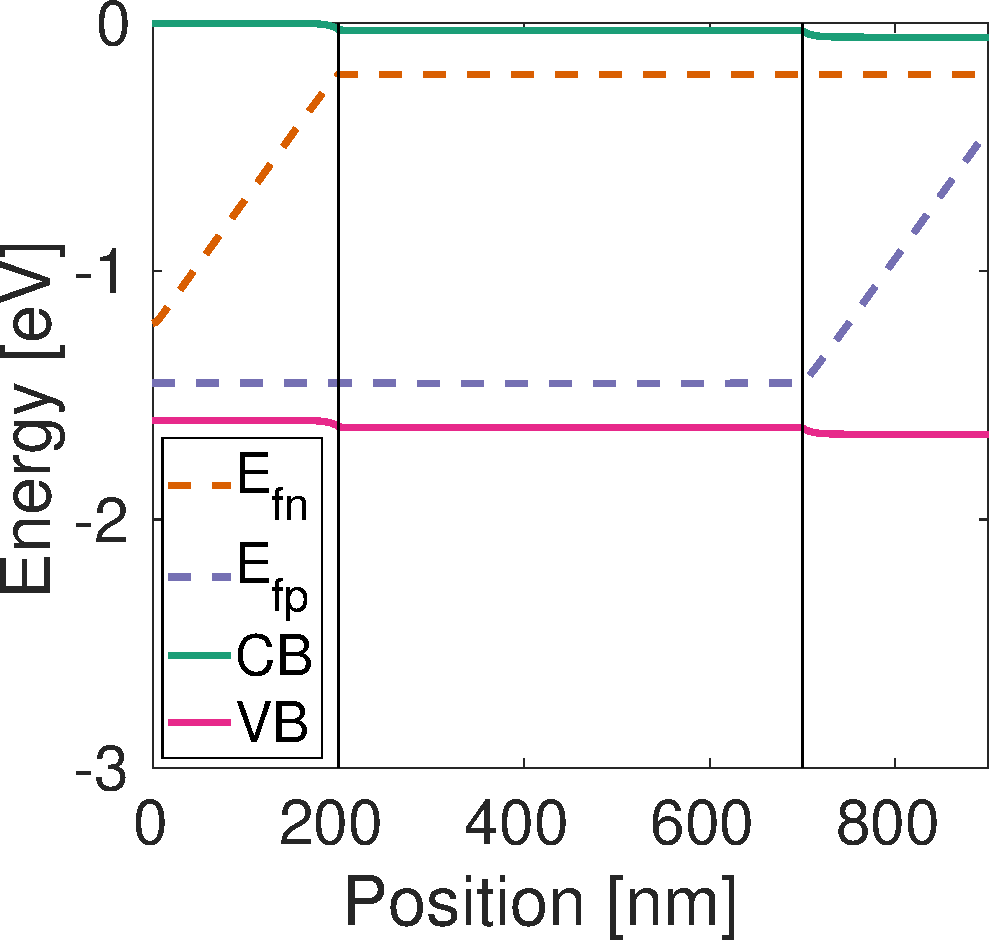
\includegraphics[width=1\textwidth]{ce_single_dd_levels/ce_ions_1000suns_levels.pdf}
						\subcaption{1000 suns, OC}\label{fig:ce_single_dd_levels-1000suns}
					\end{subfigure}

					\mycaption[Simulated energy levels in a homojunction device with mobile ions at open circuit conditions at different light intensities.]{The simulated energy levels of a homojunction $p$(\SI{200}{\nm})--$i$(\SI{500}{\nm})--$n$(\SI{200}{\nm}) device with mobile ions in the intrinsic layer. In (\textbf{a}) the device is in dark, in (\textbf{b}) it is illuminated at \SI{1}{sun} light intensity, and in (\textbf{c}) illuminated at \SI{1000}{suns}.
					}\label{fig:ce_single_dd_levels}
				}
			}
		\end{figure}

	\subsection{Interpretation of CE \textsl{versus} Light Bias With Mobile Ions}

		\paragraph{Linear part with mobile ions}\label{ce_ions_linear}
		The presence of mobile ions in perovskite materials which can accumulate at the perovskite/contacts interfaces, adds an additional capacitance $C_|ion|$, which sums up to the geometric capacitance $C_|g|$ increasing the weight of the linear component, as we showed in \authoryear{Moia2019}.
		Nevertheless, as pointed out in \cpageref{ce_limitations_perovskite}, the \acr{ce} measurements are never carried on for long enough to include the ionic migration, and so also the ionic accumulation capacitance is not observed in our experiments.
		This can be visualized with the simulation reported in \cref{fig:ce_full_dd} where the long timescale (where the current is monitored until complete stabilization) and the short timescale (few tens of microseconds) \acr{ce} experiment are compared.
		The difference between the short and long timescale extracted charges is the linear contribution by the ionic capacitance discharge, observable as electronic current thanks to the relative displacement current.
		A simulation with frozen ions (the ionic profile was stabilized at open circuit and frozen during the \acr{ce} experiment) was also performed but not reported, the extracted charge is identical to the reported short timescale extraction simulation.

		EXPLAIN HOW THE SHORT TIME EXTRACTION CORRESPONDS TO A LARGE CAPACITOR WITH ELECTRODES IN THE CONTACTS; SENSITIVE TO THE PEROVSKITE THICKNESS; WHILE THE LONG TIMES ONE IS SENSITIVE TO THE JUNCTION/TRANSITION CAPACITANCE ONLY

		\begin{figure}%[!hbtp]%
			\makebox[\textwidth][c]{
				\parbox{1.1\textwidth}{
					\centering
					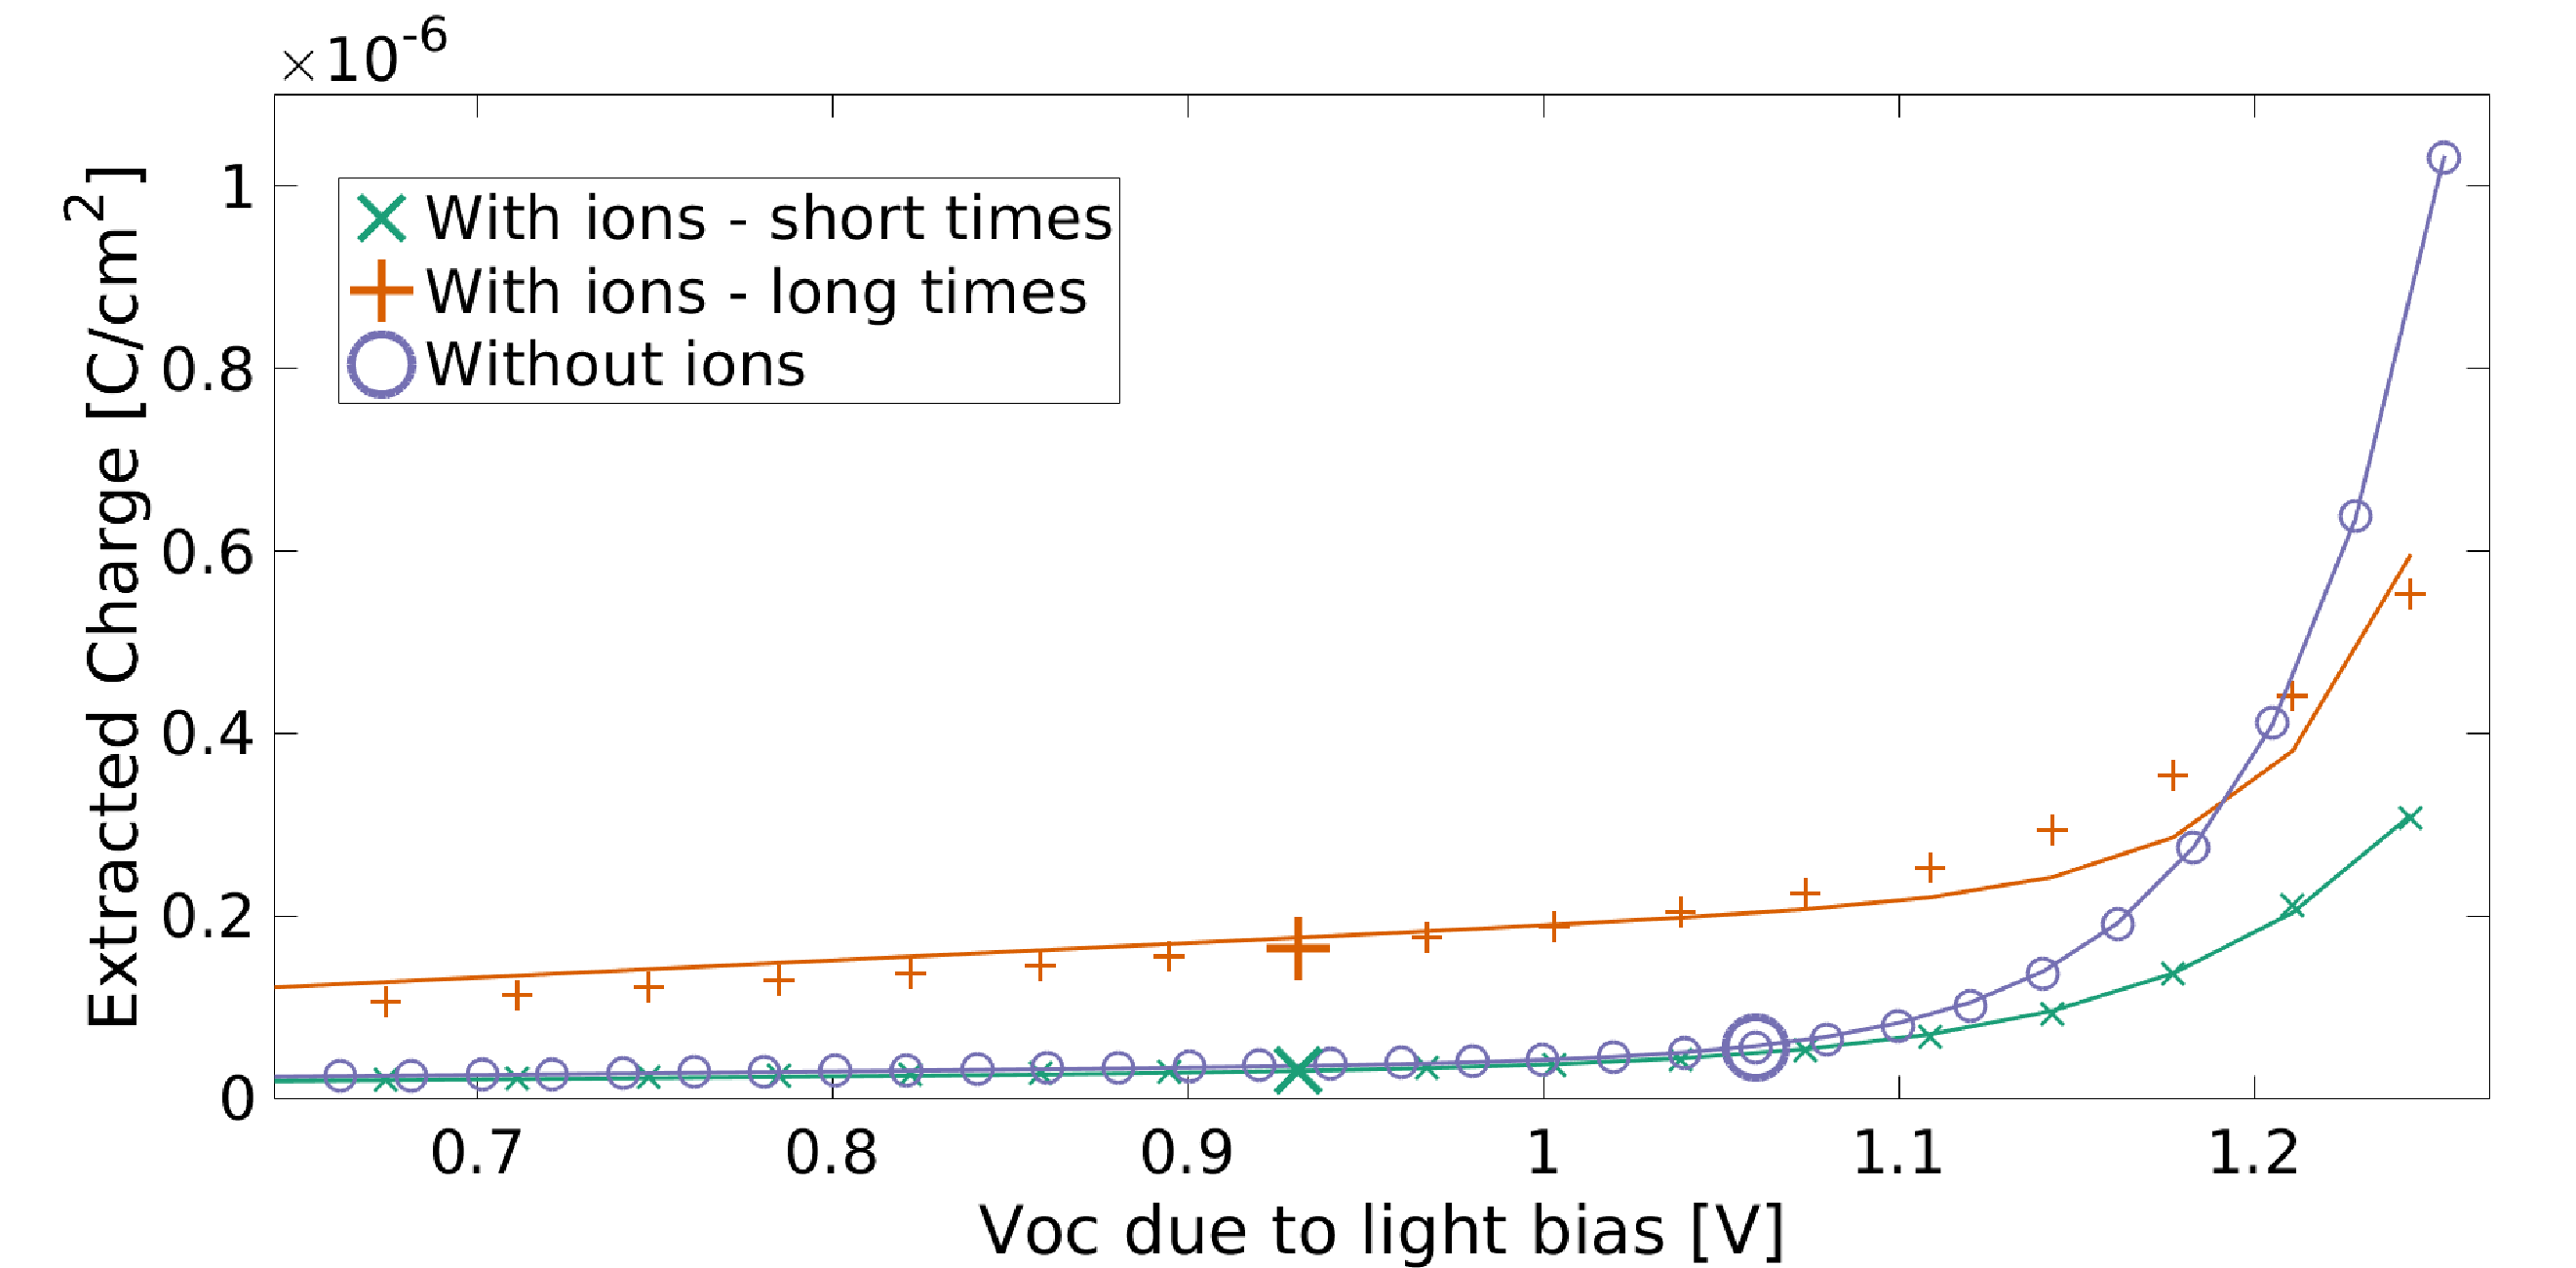
\includegraphics[width=0.9\textwidth]{ce_full_dd/ce_full_dd.pdf}
					\mycaption[Simulation of a complete CE experiment: charge \textsl{versus} light bias with or without mobile ions.]{
						A simulation for a homojunction device up to 1000~sun illumination (rightmost point of each set) is reported, with three points for decade.
						For each set of points, the bigger size one indicates the 1~sun pre\hyp{}illumination.
						The green crosses simulates the experimentally utilised conditions: the charge gets integrated over few microseconds, while the mobile ions didn't have enough time to start migrating.
						The orange pluses considers the charge integrated until the device stabilization, over various seconds, including also the ionic displacement current.
						The purple circles simulates a mobile ions free device.
						The solid lines represents the linear plus exponential fit crossing (0,0) obtained with the \cref{eq:ce_full} $n_|CE| = C_|g| V + n_|eq| \{\exp[q V / (mk_|B|T)] - 1\}$ where $C_|g|$, $n_|eq|$, and $m$ are free fitting parameters whose meaning is described in the text.}\label{fig:ce_full_dd}
				}
			}
		\end{figure}

		\paragraph{Exponential part with or without mobile ions}
		As can be seen in \cref{fig:ce_full_dd}, the simulated geometric capacitance is similar to the one obtained from short time extraction with mobile ions but the exponential part is considerably different.
		%		when a device with no mobile ions is simulated, longer extraction time doesn't result in more charge, as expected due to the suppression of the ionic contribution.
		This is caused by the very different free charge accumulation profile: the presence of an un\hyp{}shielded electric field in the absorber layer causes the free carriers to accumulate close to the respective selective layer, in other words it keeps the charges away from the respective recombination centres (\textsl{e.g.}\ perovskite/\gls{htm} for electrons).
		This allows the simulated ions free device to store more charge at the same illumination intensity.

		\FloatBarrier
		\newpage
\section{Transient PhotoVoltage (TPV)}
	\epigraph{\textit{\enquote{Imma firin mah lazor\\pewpew pewpewpew}}}

	\paragraph{Concept}
	%	While a complete device is kept open circuit under constant illumination, a small extra illumination is added \textsl{via} a short laser pulse.
	This technique allows us to perturb and observe a solar cell device at open circuit under illumination.
	We perturb the device photo\hyp{}generating an additional small amount of charge and we observe the perturbed open circuit voltage dynamics.
	The \gls{voc}, originally at its steady state value, will increase due to the greater generation rate during the laser pulse.
	%	From the \gls{voc} \textsl{versus} illumination relation for photodiodes reported in \cref{eq:voc_vs_phi} follows that the \gls{voc}, at this new higher illumination, increases (this is not always the case, as for non-stabilized perovskite solar cells \cite{Calado2016}).
	After the end of the short pulse, the \gls{voc} will slowly go back to the steady state value relative to the constant illumination.
	The dynamics of this \gls{voc} relaxation back to the steady state value is the focus of Transient PhotoVoltage experiments (also known as PhotoVoltage Decay experiments) which has been applied to \gls{osc} \cite{Shuttle2008}, to \gls{dssc} \cite{ORegan2005,ORegan2004,ORegan2006}, and recently also to perovskite solar cells \cite{Roiati2014a,Marin-Beloqui2014}.
	From this kinetic profile, a charge life\hyp{}time can be obtained and plotted against the light bias due to the constant background illumination, as in the example of \cref{fig:tpv-monoexp}.
	This gives us information about the dominant recombination rate and its dependence on the light bias.

	\begin{SCfigure}
		\centering
		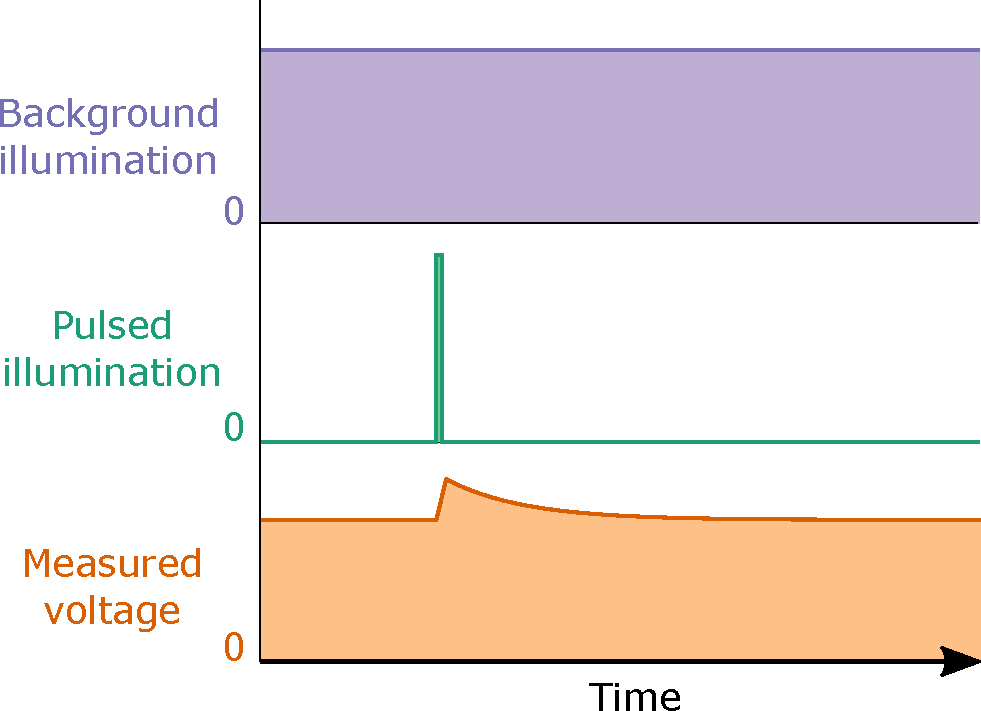
\includegraphics[width=0.55\textwidth]{tpv_scheme/tpv_scheme.pdf}
		\mycaption[Scheme of TPV experiment.]{
			A pulsed illumination sums on the constant background illumination, the measured open circuit voltage dynamic shows an increase and a relaxation. }\label{fig:tpv_scheme}
	\end{SCfigure}

	\paragraph{Procedure}
	The device is kept under constant illumination by a white \gls{led} ring at open circuit until stabilization is reached.
	Failure to reach stabilization of the ionic profile will affect the measurement results \cite{ORegan2015b} and can cause unexpected negative \acr{tpv} peaks \cite{Calado2016}.
	Then an additional short illumination pulse is provided using a nitrogen laser.
	The pulse duration (\SI{\approx 1.5}{\ns}) is shorter than the oscilloscope resolution we usually employ, so we assume that the measurement happens when the pulse is already over.
	In the literature, this is not always the case as other research groups use a \gls{led} diode for the pulsed illumination \cite{Calado2016}.
	Usually a wavelength of \SI{590}{\nm} is selected using a Rhodamine 6G solution \cite{RadiantDyesLaser}, this wavelength illuminates in depth the perovskite layer (in contrast to a blue light where the illumination would be absorbed within the first hundreds of nanometres of the material \cite{Bi2016,Tress2016}).
	During all the process, the device is connected to an oscilloscope, registering the open circuit voltage profile (the \SI{1}{\Mohm} resistance of the oscilloscope is a good approximation of open circuit).
	The voltage profile gets averaged over a few tens of pulses in order to increase the signal to noise ratio.
	Initially the light illumination is set to \SI{1}{sun} and the laser pulse intensity is attenuated using a neutral filter so that the voltage perturbation remains smaller than \SI{10}{\mV} for ensuring the small perturbation regime.
	The measurement is repeated after decreasing the background light intensity and waiting a stabilization time.
	The fitted small perturbation life\hyp{}time is plotted \textsl{versus} the light bias.
	The background illumination is decreased down to dark background illumination over a few tens different intensities.
	1~sun equivalent illumination is defined as the illumination at which a silicon photodiode gives the same \gls{jsc} as under calibrated 1~sun from the solar simulator.

	\paragraph{Noise treatment}\label{tpv_robust}
	Most of the observed noise (\SI{< 2E-7}{\s}) is due to the radiofrequency emitted by the spark in the nitrogen laser which gets received by all the non\hyp{}coaxial cables (coaxial ones do not) and from the circuitry of the samples holder acting as an antenna.
	On the contrary to what happens for \acr{ce} (see \cpageref{ce_noise}), the short times noise does not follow a constant pattern, so averaging the measurement over a few repetitions (usually 30) manages to reduce the noise.
	This noise can affect the exponential or bi\hyp{}exponential fitting, for this reason a robust fitting routine has been used, which gives a lower weight to outlier points.
	An example can be seen in \cref{fig:tpv_robust}.

	\begin{figure}
		\makebox[\textwidth][c]{
			\parbox{1.1\textwidth}{
				\centering
				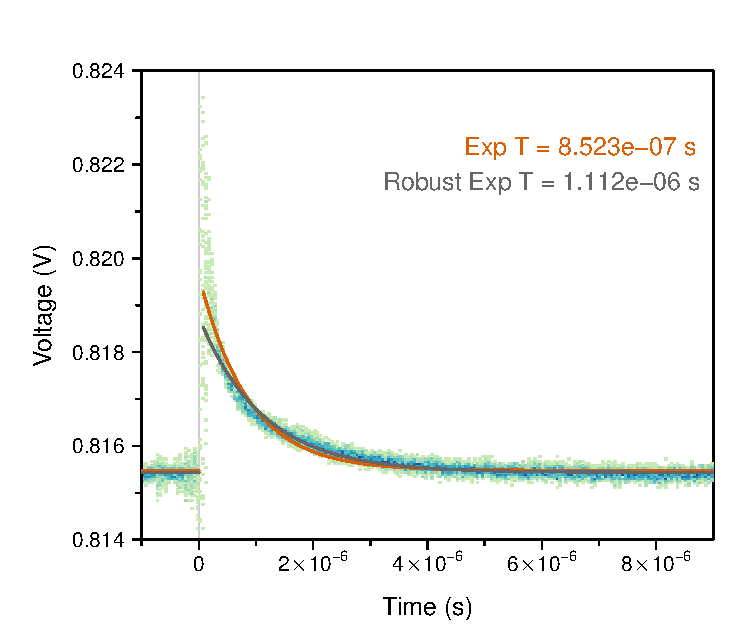
\includegraphics[width=0.8\textwidth]{{tpv_robust/TPV_ig101-1555-1_0.815394_V-monoexp}.pdf}
				\mycaption[Robust and normal fitting comparison.]{Plot of a voltage profile from a single \gls{tpv} decay.
					The 12500 voltage points are represented in a 2D histogram for avoiding the overplotting problem.
					The normal non\hyp{}linear least squares fitting (in orange) is affected by initial noise (a faster decay if we consider this as a bi\hyp{}exponential decay), outliers and characteristics not of interest by the model.
					The non\hyp{}linear robust fitting (in magenta) manages to reduce the weight of these points.
					The studied device is a \gls{fto}\-/\ch{d-TiO2}\-/\acr{csfamapbibr}\-/\gls{tae4}\-/Au \cite{Gelmetti2019} with 1~sun background illumination.}\label{fig:tpv_robust}
			}}
	\end{figure}

	\paragraph{Importance of stable steady state starting point}\label{tpv_negativePeaks}
	The values extracted from \acr{tpv} are strongly sensible to the surface recombination and electric fields in the absorber, which in turn vary during ionic profile stabilization.
	Comparison of decay times with different stabilization times can be found in \authoryear{ORegan2015b}, while in \authoryear{Calado2016} even negative peaks are reported and explained with the presence of a residual electric field in the absorber previous to ionic profile stabilization.

	\paragraph{Small perturbations regime}\label{tpv_perturbation}
	The intensity of the laser pulse is attenuated using a variable neutral density filter (a partially reflecting wheel with different positions for different transmittivities) so that the voltage perturbation caused by the light pulse does not exceed \SI{10}{\mV} with 1~sun background illumination intensity.
	We consider this a "small\hyp{}enough" perturbation with regards to the measured \gls{voc} (see \cpageref{perturbation} for a definition of small perturbation).
	For example, comparing the excess charge in a \gls{fto}\-/\ch{d-TiO2}\-/\acr{csfamapbibr}\-/\gls{spiro}\-/Au solar cell at \gls{voc} and at \gls{voc}~+~\SI{10}{\mV} which can be obtained from the data in \cref{fig:ce_noise-integrateExp} fitted with \cref{eq:ce_full} we can obtain respectively a value of \SI{8.2E-8}{} and \SI{8.9E-8}{\coulomb\per\square\cm}.
	%Even if we're not considering the dark charge concentration (not measurable in a \acr{ce} experiment), the smallness of the charge perturbation is arguable.
	A smaller perturbation is not practically doable as we are limited to \SI{> 3}{\mV} perturbations due to the strong noise observed in this transient measurement.
	%Clearly, the pulse intensity which could be considered a "small-enough" perturbation at high background illumination is not small any more at lower illumination and definitively cannot be small at dark background conditions.
	Decreasing the background light bias, the laser light pulse intensity is kept constant even when it gets out from small perturbation regime, this is needed in order to be able to use the \acr{tpv} data for calculating \acr{dc}, as explained in \cpageref{dc_perturbation}.
	%We could regulate the pulse intensity depending on the background light intensity, to ensure its smallness, but we \emph{do not} do this in order 
	This does not affect the parameter extraction from \acr{tpv} as just the high illumination intensity points are considered, as seen in \cpageref{tpv_tau_vs_intensity}, in order to study the device close to its expected working conditions.

	\subsection{Interpretation of TPV Mono\hyp{}Exponential Decays}

		\paragraph{Voltage transient and charge concentration relationship}
		As we assume to be in the small perturbation regime, we can study the \cref{eq:ce_full} up to the first term of its series expansion:
		\begin{dmath}
			n(V_0 + \Delta V) \approx n(V_0) + \Delta V \cdot \left.\frac{\partial n}{\partial V}\right\rvert_{V=V_0} = n(V_0) + \Delta V \cdot \left[C_|g| + \frac{n_|eq| q}{mk_|B|T}\exp(\frac{qV_0}{mk_|B|T})\right]
			%		n(V_0 + \Delta V) \approx n(V_0) + \Delta V \cdot \eval{\dv{n}{V}}_{V=V_0} = n(V_0) + \Delta V \cdot \left(C_|g| + \frac{n_|eq| q}{mk_|B|T}\exp\left(\frac{qV_0}{mk_|B|T}\right)\right)
		\end{dmath}
		Assigning the last addend to $\Delta n$ we can see that the charge amount variation not only is linear with $\Delta V$ (as we're in the small perturbation regime), but it also depends on the steady state voltage $V_0$.
		This relation is studied in the differential capacitance (\acr{dc}) experiment, described further in this chapter.

		\paragraph{Voltage re\hyp{}equilibration dynamics}
		For what concerns a \acr{tpv} experiment, we are just interested in the analysis of the time needed for re\hyp{}equilibration to steady state conditions.
		As aforementioned, the relation between $\Delta V$ and $\Delta n$ in small perturbation regime is linear, so the lifetime extracted from a $\Delta V$ decay will have the same lifetime of the underlying $\Delta n$, which is the interesting quantity when speaking of recombination.
		This means that we can observe the variations in voltage for having a correct kinetic description of the charge amount variation.
		At steady state conditions, the time derivative of the amount of charge is zero $\partial n_0 / \partial t = g(\phi) - U(n_0) = 0$ where $g$ is the generation rate and $U$ is the recombination rate.
		Considering the situation after the end of the light pulse, so while $g$ is constant but $n$ has been increased by $\Delta n$, and using a simplified expression for the recombination including just two contributions with reaction order 1 and 2 and rate constants $k_1$ and $k_2$ we can write:
		\begin{dmath}
			%		\frac{\partial (n_0 + \Delta n)}{\partial t} = g - k_1(n_0 + \Delta n) - k_2(n_0 + \Delta n)^2 = (g - k_1 n_0 - k_2 n_0^2) - (k_1 \Delta n + 2 k_2 n_0 \Delta n) - (k_2 \Delta n ^2) \approx - (k_1 + 2 k_2 n_0 ) \Delta n
			\pdv{(n_0 + \Delta n)}{t} = g - U = g - k_1(n_0 + \Delta n) - k_2(n_0 + \Delta n)^2 = (g - k_1 n_0 - k_2 n_0^2) - (k_1 \Delta n + 2 k_2 n_0 \Delta n) - (k_2 \Delta n ^2) \approx - (k_1 + 2 k_2 n_0 ) \Delta n
		\end{dmath}
		where the zeroth order term is the steady state value, so it's zero, and the second order order term can be neglected (if $\Delta n \ll n_0$ then $k_2 \Delta n^2 \ll k_2 n_0 \Delta n$).
		So the rate equation is a simple pseudo first order reaction, and the kinetic behaviour follows an exponential description like:
		\begin{equation}\label{eq:tpv_monoexp}
			n (t) = n_0 + \Delta n_0 \cdot e^{-(k_1 + 2 k_2 n_0) t} = n_0 + \Delta n_0 \cdot e^{-t / \tau}
		\end{equation}
		where $\tau = (k_1 + 2 k_2 n_0)^{-1}$ is the small perturbation life\hyp{}time.
		For a single recombination with a generic recombination reaction order $\Phi$ we can generalize to \cite{Shuttle2008}:
		\begin{equation}\label{eq:tpv_tau_order}
			\tau \approx (\Phi k n_0^{\Phi-1})^{-1}
		\end{equation}
		where $k$ is the dominant recombination rate constant.

		\begin{figure}
			\makebox[\textwidth][c]{
				\parbox{1.1\textwidth}{
					\centering
					\begin{subfigure}[t]{0.5\textwidth}
						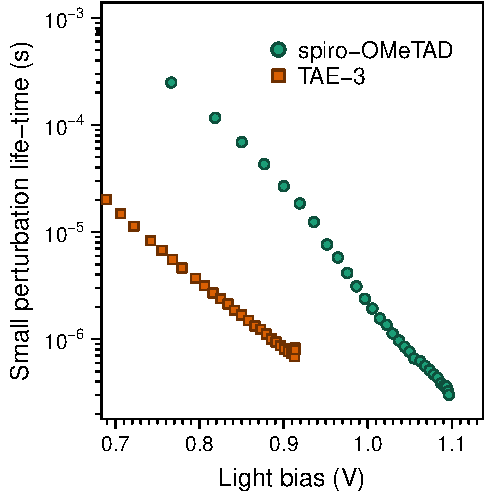
\includegraphics[width=1\textwidth]{tpv/monoexp/spiro_vs_TAEs-TPVs-robustmonoexp-crop.pdf}
						\subcaption{Mono\hyp{}exponential life\hyp{}times \textsl{versus} light bias}\label{fig:tpv-monoexp}
					\end{subfigure}
					\qquad
					\begin{subfigure}[t]{0.5\textwidth}
						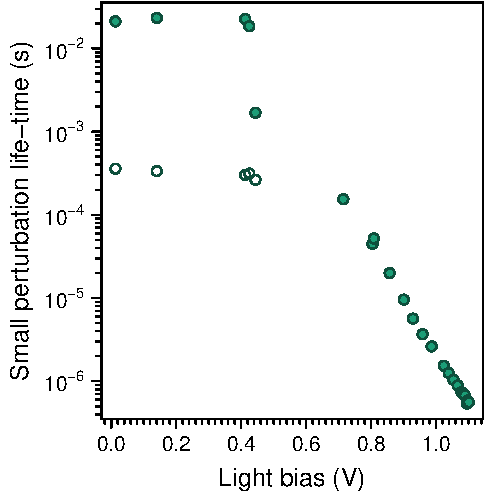
\includegraphics[width=1\textwidth]{tpv/biexp/tpv-tpv-mixedbimono-crop.pdf}
						\subcaption{Bi\hyp{}exponential life\hyp{}times \textsl{versus} light bias for a \gls{famapbibr} device}\label{fig:tpv-biexp_full}
					\end{subfigure}
					\bigskip

					\begin{subfigure}[t]{0.6\textwidth}
						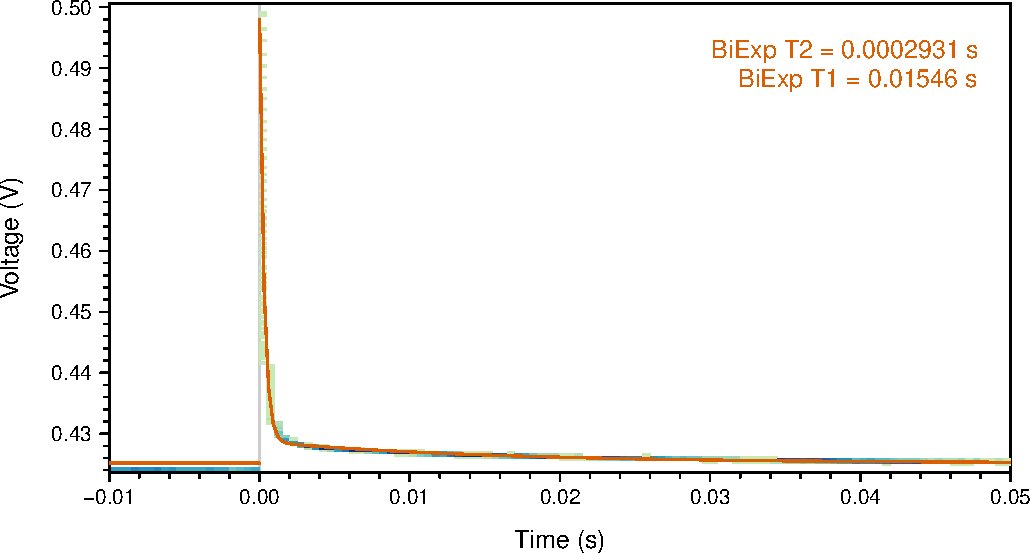
\includegraphics[width=1\textwidth]{{tpv/biexp/tpv/TPV_ig57-475-2_0.424021_V-biexp-crop}.pdf}
						\subcaption{Single bi\hyp{}exponential decay}\label{fig:tpv-biexp_single}
					\end{subfigure}

					\mycaption[Example of life\hyp{}times \textsl{versus} light bias plot obtained from a TPV experiment.]{In (\textbf{a}) the small perturbation life\hyp{}times obtained from robust mono\hyp{}exponential fitting are plotted against light bias for \gls{fto}\-/\ch{d-TiO2}\-/\acr{csfamapbibr}\-/\gls{htm}\-/Au devices \cite{Gelmetti2019}. In (\textbf{b}) the life\hyp{}times of a \gls{fto}\-/\ch{d-TiO2}\-/\acr{famapbibr}\-/\gls{spiro}\-/Au device as obtained from a robust bi\hyp{}exponential fitting for low light bias, where the decays are clearly biphasic, and mono\hyp{}exponential for higher illuminations. In (\textbf{c}) the full data for the point at \SI{0.42}{V} from (\textbf{b}) is reported.}\label{fig:tpv}
				}
			}
		\end{figure}

	\subsection{Interpretation of TPV Bi\hyp{}Exponential Decays}

		\paragraph{At high background illumination}
		For some devices, rather than an exponential decay, a bi\hyp{}exponential voltage decay is observed, like the one reported in \cref{fig:tpv-biexp_single}.
		This is more frequent in bottom cathode devices including mesoporous titania layers \cite{Carnie2015,ORegan2015b,Bertoluzzi2015} but has also been reported for silicon solar cells \cite{Kiermasch2018}.
		With \emph{bi\hyp{}exponential} decay we refer to the sum of two exponential decays with two different half\hyp{}life times, like:
		\begin{equation}\label{eq:tpv_biexp}
			V (t) = V_0 + \Delta V_a \cdot e^{-t/\tau_a} + \Delta V_b \cdot e^{-t/\tau_b}
		\end{equation}
		where $\tau_a$ and $\tau_b$ are two distinct life\hyp{}times while $\Delta V_a$ and $\Delta V_b$ are the respective amplitudes of the contributions to the measured decay.
		The presence of two different recombination processes is not enough for justifying a bi\hyp{}exponential decay.
		This is clear looking to \cref{eq:tpv_monoexp}, where considering two recombination processes with two different reaction orders we obtained a simple exponential decay.
		What we have to remember here, is that \cref{eq:tpv_monoexp} was obtained for a zero dimensional case, like what would happen in a homogeneous chemical reaction.
		In our case, the multiple recombination centres could be spatially separated.
		If the charge concentration in the two centres is dis\hyp{}entangled (is not identical at any time), the sum of two exponential decays can be expected rather than a simple exponential.
		This dis\hyp{}entanglement is possible if the time needed for the free carriers to migrate from a recombination centre to the other is larger than the shorter recombination life\hyp{}time.
		This can happen thanks to a large\hyp{}enough distance between recombination centres together with a slow free carriers mobility \cite{Calado2018}.
		For example for recombination centres at different depths in the solar cell stack, like at the two perovskite/contacts interfaces.
		The fact that the presence of mesoporous structures are often present when bi\hyp{}exponential decays are observed can be understood by the smaller mobility of perovskite when intercalated in such structures \cite{Leijtens2014}.
		This have been reported also for laterally distanced recombination centres (\textsl{e.g.} pinholes \textsl{versus} well covered regions) by \authoryear{Montcada2017}.
		%	the high mobility in the electrodes is expected to equal the quasi-Fermi levels in the two adjacent recombination centres avoiding bi\hyp{}exponential decays, nevertheless reports of this phenomena have been reported \cite{Montcada2017}.

		\paragraph{Mobility limited case}\label{tpv_mobility}
		As we just saw, the mobility is a crucial parameter for the \acr{tpv} experiment.
		As a mental exercise we can imagine a case where the mobility is so slow that the free charges take a long time to diffuse (we consider diffusion as perovskite solar cells are assumed to be field\hyp{}free in the absorber layer, but the same concept would hold with charges' drift) from the generation zone (in the absorber) to the recombination centre (\textsl{e.g.} at a contact/absorber interface).
		In such an extreme case the provisioning of charges to the recombination centres could become a bottleneck rather than the recombination itself.
		A drift\hyp{}diffusion simulation of this can be found in \authoryear{Calado2018}.
		In this regime, a \acr{tpv} experiment would be rather insensitive to actual recombination constants and even to light intensity, giving just information about mobility.
		As the observed \acr{tpv} life\hyp{}times are strongly light\hyp{}intensity dependent, at least at high background illumination, we can exclude to be in this mobility\hyp{}limited regime.
		This would have to be revised in case a strong illumination\hyp{}dependent mobility in perovskite materials was demonstrated, as has been reported in \gls{osc} \cite{Eng2010,Shuttle2010,Deledalle2014}.
		Also a slow trapping and de\hyp{}trapping of the carriers can result in a reduced and illumination\hyp{}dependent mobility \cite{Du2018}.

		\paragraph{Inhomogeneous charge concentration profiles}
		Due to the internal electric field, the free carriers concentration can be inhomogeneous.
		For the surface recombination, this implies that the average excess carriers concentration obtained from \acr{ce} is not necessarily the carriers concentration at the recombination centre \cite{Kirchartz2012}.
		For the band\hyp{}to\hyp{}band recombination, this implies that the $n \cdot p$ product, integrated over the device thickness, can be much smaller than an homogeneous carriers concentration \cite{Deibel2009}.
		These considerations are key for drift\hyp{}driven \gls{osc} with low doping level materials \cite{Deledalle2015,Deledalle2014} but should be of smaller impact for the diffusion\hyp{}driven, field free perovskite solar cells, at least at steady state when the internal electric field is mostly shielded by the ionic accumulation at the interfaces.

		\paragraph{At low background illumination -- large perturbations}
		While bi\hyp{}exponential decays at high background illumination are often not observed, these are quite always present at lower background illumination, as in for the example reported in \cref{fig:tpv-biexp_full}.
		Clearly, the aforementioned explanation for bi\hyp{}exponential decays at high illumination are still valid for the low illumination case.
		Additionally, when studying a decay measured at very low background light intensity, we have to remember that we're out of the small perturbation regime and this could justify non\hyp{}exponential decays in various ways.


		\begin{figure}
			\makebox[\textwidth][c]{
				\parbox{1.1\textwidth}{
					\centering
					\begin{subfigure}[t]{0.51\textwidth}
						\centering
						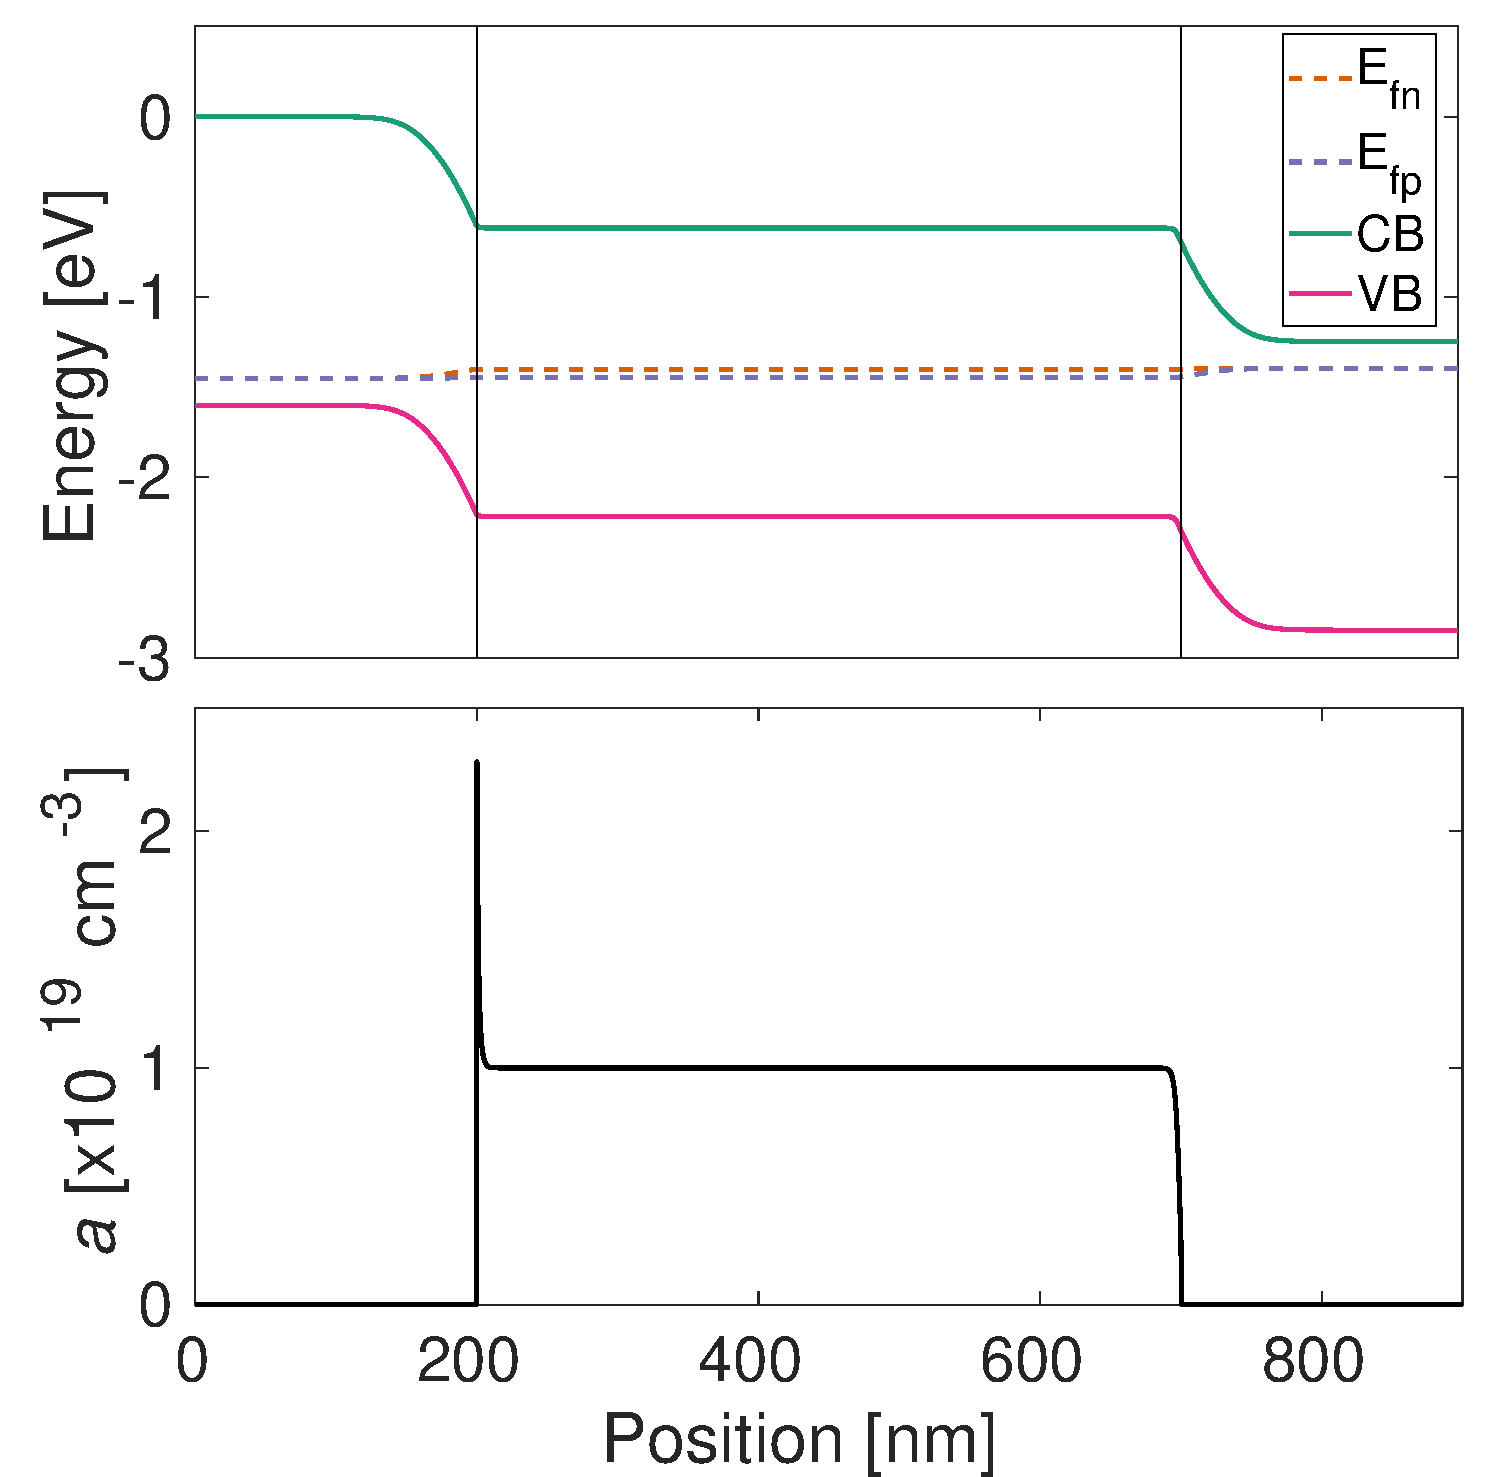
\includegraphics[width=0.9\textwidth]{tpv_ionic/tpv_ionic_reference.pdf}
						\subcaption{Low illumination, steady state.}\label{fig:tpv_ionic-reference}
					\end{subfigure}
					\qquad
					\begin{subfigure}[t]{0.51\textwidth}
						\centering
						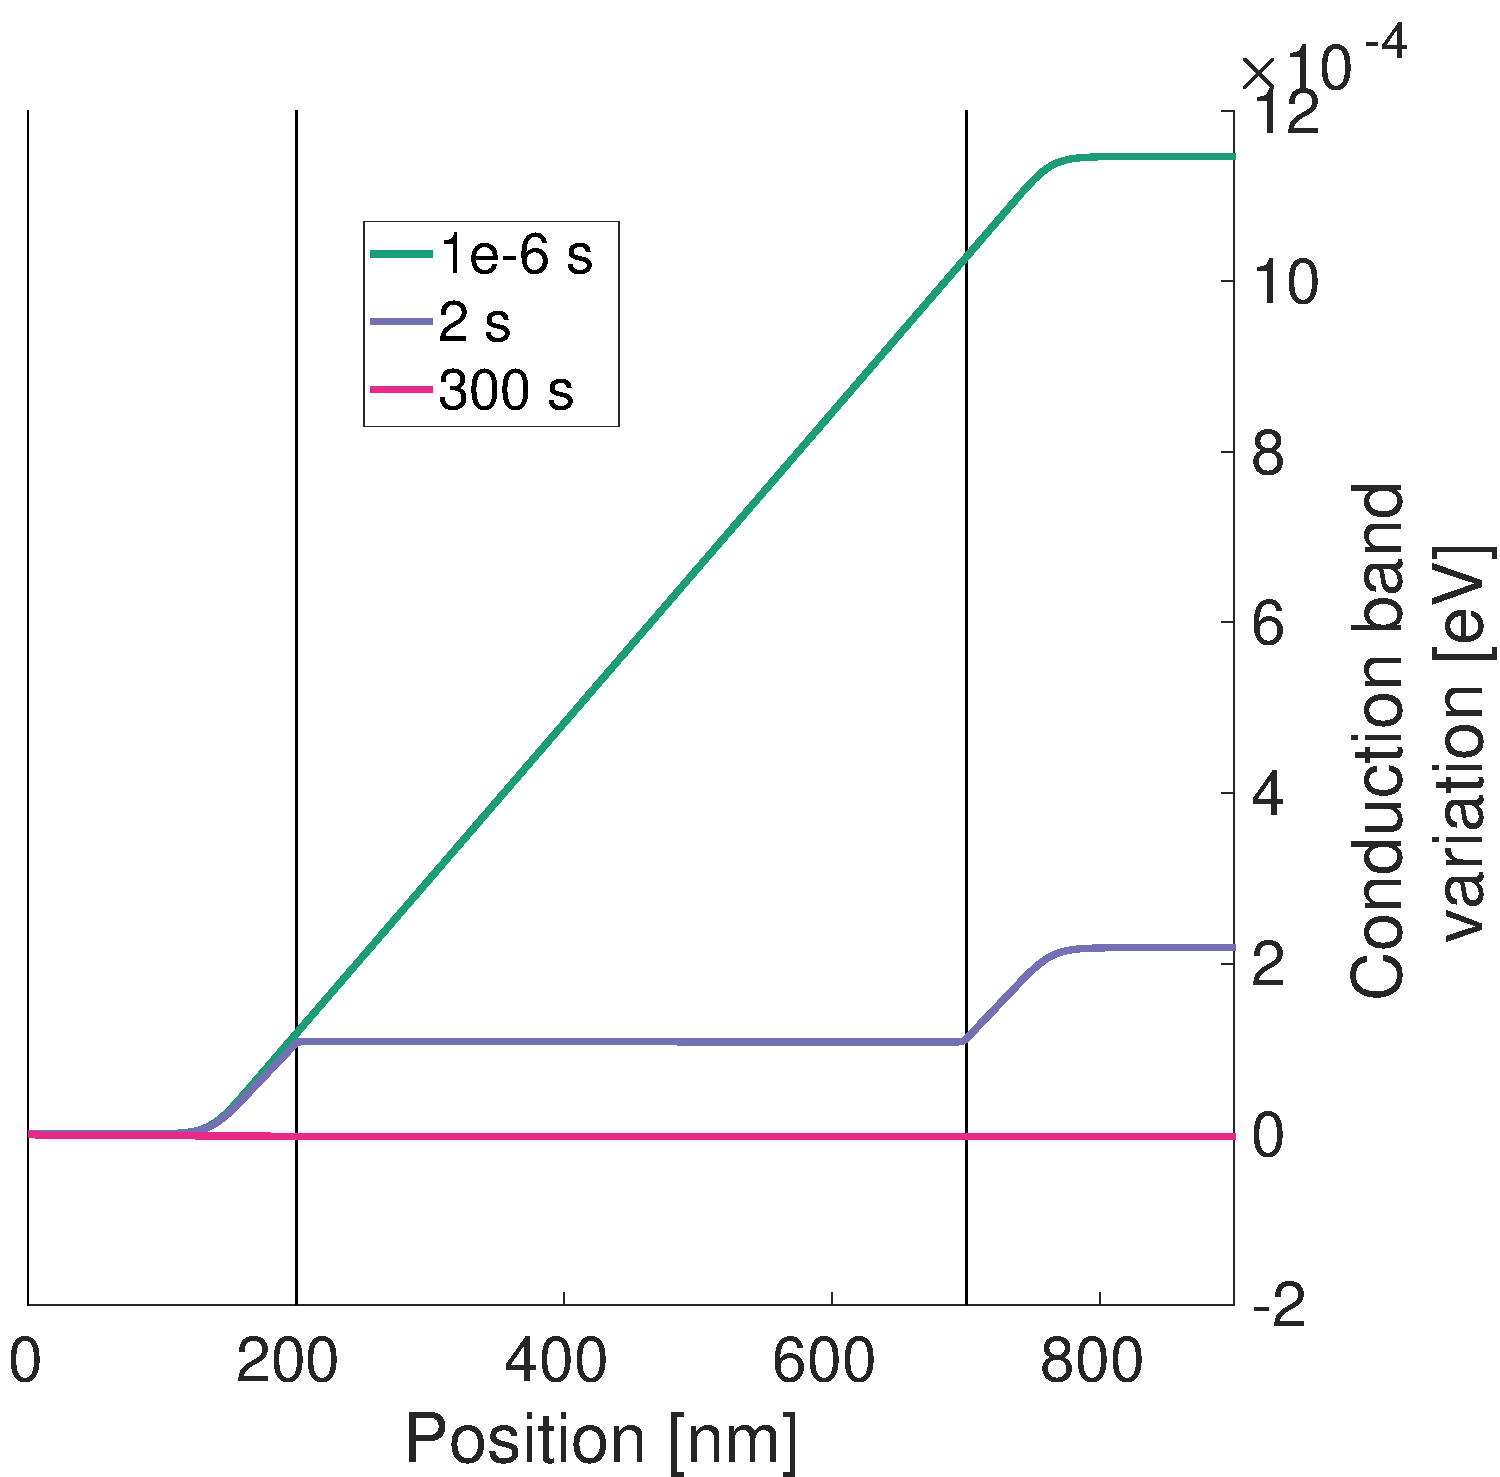
\includegraphics[width=0.9\textwidth]{tpv_ionic/tpv_ionic_cb.pdf}
						\subcaption{Conduction band variation over time.}\label{fig:tpv_ionic-cb}
					\end{subfigure}
					\bigskip

					\begin{subfigure}[t]{1\textwidth}
						\centering
						\includegraphics[width=0.8\textwidth]{tpv_ionic/tpv_ionic_dynamics.pdf}
						\subcaption{Voltage, charge, and ionic accumulation variation over time.}\label{fig:tpv_ionic-dynamics}
					\end{subfigure}
					\mycaption[Simulation of TPV at low background intensities with mobile ions.]{
						A TPV experiment has been simulated on a $p$(\SI{200}{\nm})--$i$(\SI{500}{\nm})--$n$(\SI{200}{\nm}) homojunction device with mobile ions in the absorber layer and at open circuit conditions.
						Low background light intensity \SI{1e-8}{suns} was applied, corresponding to a light bias of \SI{53}{\mV}.
						The illumination pulse was \SI{1e-8}{s} long and weak enough to cause a perturbation which can be considered small.
						In (\textbf{a}) the steady state energy levels and ionic profile is shown.
						In (\textbf{b}) the variation, taking the steady state profile as zero, of the conduction band during a TPV experiment.
						In (\textbf{c}), over time I plotted: the bi\hyp{}exponential voltage decay; the normalized total charge variation (the electronic profile integrated over the device thickness); and the ionic concentration variation at the perovskite/\gls{etm} interface, where the low ionic concentration temporarily increases during the transient.
						The represented data is interpreted in \cpageref{tpv_biexp_lowlight_ions}.
					}\label{fig:tpv_ionic}
				}
			}
		\end{figure}

		\paragraph{At low background illumination -- ionic migration}\label{tpv_biexp_lowlight_ions}
		At low light intensity, the free carriers density can be very small, so that the recombination can be very slow.
		At these long times, another process of perovskite solar cells can be active: ionic migration.
		%	at the very long time scale of the recombination at low free carriers density (low background illumination)
		What I have observed, simulating a \acr{tpv} experiment on a homojunction device with mobile ions in the absorber layer, is that ionic profile can update to the pulse\hyp{}perturbed cell condition before the extra free charges recombine, in case this is very slow.
		In \cref{fig:tpv_ionic-reference} the steady state energy levels and ionic accumulation at the perovskite/contact interfaces is represented.
		In \cref{fig:tpv_ionic-cb} the variations of the conduction band profile are plotted.
		Here we can see that at \SI{1e-6}{s} the CB varies due to the new charges photo\hyp{}generated by the laser pulse, the non-flat conduction band indicates the presence of an electric field in the perovskite layer.
		At the same times, we can see in \cref{fig:tpv_ionic-dynamics} the increase in the total amount of electrons in the device due to the laser photo-generation which is reflected also by the open circuit voltage increase, as expected for a \acr{tpv} experiment.
		Then from \SIrange{1e-3}{1e-1}{s}, the ionic profile completely screens out the electric field.
		In \cref{fig:tpv_ionic-cb} this is visible as a flattening of the conduction band in the perovskite, this simple displacement of ions decreases the electrostatic potential at the \gls{etm}.
		In absence of changes in the charge density, a shift in the electrostatic potential in the \gls{etm} causes an identical shift in the quasi-Fermi levels in the \gls{etm}.
		As the voltage is defined as $V = E_|fn|^{\mathrm{ETM}} - E_|fp|^{\mathrm{HTM}}$ this shift clearly gets reflected in a voltage change.
		In the same time span, in \cref{fig:tpv_ionic-dynamics} we can see how the ionic concentration at an interface changes and how this gets reflected on the open circuit voltage, without any change in the total charge concentration.
		Finally, at longer times the laser\hyp{}generated free charges slowly recombine (the ionic profile just catches up this free charges variation), the CB returns to its steady state profile and a second decay is observed in the open circuit voltage.
		So, in this case, only the slow decay is actually related to charge recombination, while the fast one is just due to the ionic profile update.
		%	This causes a first exponential decay of the voltage, followed by a second exponential decay due to the actual recombination of the charges generated by the laser pulse.
		This means that, if the simulation is correct, at low background light intensities we can obtain information on the ionic mobility and concentration from the fast component of bi\hyp{}exponential \gls{tpv} decays.
		%	The line at \SI{1e-6}{s} represents the CB just after the photo-generation of charges from the laser pulse; at \SI{2}{s} the ionic profile completely screened out the electric field; at longer times the generated free charges recombines and the CB returns to its steady state profile. 

		\begin{figure}
			\makebox[\textwidth][c]{
				\parbox{1.1\textwidth}{
					\centering
					\begin{subfigure}[t]{0.5\textwidth}
						\includegraphics[width=1\textwidth]{tpv_full_dd/tpv_full_dd_noions.pdf}
						\subcaption{Without mobile ions}\label{fig:tpv_full_dd_noions}
					\end{subfigure}
					\qquad
					\begin{subfigure}[t]{0.5\textwidth}
						\includegraphics[width=1\textwidth]{tpv_full_dd/tpv_full_dd_ions.pdf}
						\subcaption{With mobile ions}\label{fig:tpv_full_dd_ions}
					\end{subfigure}
					\mycaption[Simulated \glsentryshort{tpv} without and with mobile ions.]{
						The \gls{tpv} of a homojunction solar cell is simulated, with background illumination from \SIrange{1e-10}{1}{suns} (respectively the leftmost and the rightmost points) with 3 points per decade.
						The pulse intensity was regulated in order to not exceed \SI{8}{\mV} of perturbation.
						In (\textbf{a}) a device without mobile ions is simulated, the resulting decay is a simple exponential, so the life\hyp{}time of an exponential fit is reported.
						In (\textbf{b}) a device with mobile ions in the absorber layer is reported, the resulting decay is a simple exponential at high light biases but a bi\hyp{}exponential at lower background illuminations, so the two life\hyp{}times from a bi\hyp{}exponential fitting are reported.
					}\label{fig:tpv_full_dd}
				}}
		\end{figure}

		\paragraph{At low background illumination -- fast life\hyp{}time plateau}
		Both the fast and the slow component of bi\hyp{}exponential decays hit a maximum value (plateau) at very low light intensities.
		Looking at the fast component, assigned to the rearrangement of the ionic profile, we usually observe a constant life\hyp{}time.
		This points to a background light insensitive ionic rearrangement time constant, which implies a constant ionic mobility.
		This should be further studied considering the report of illumination-dependent ionic mobility by Maier's group in \authoryear{Kim2018}.

		\paragraph{At low background illumination -- slow life\hyp{}time plateau}
		The slow decay component at very low background light intensity has been assigned to the electronic recombination.
		In drift-diffusion simulations, the life\hyp{}time does not show a maximum value and grows as the light intensity is decreased.
		But in the actual experiment setup, decays life\hyp{}times are limited at long times by the discharge of the through the oscilloscope resistance and through the device shunt resistance, whatever is the fastest.
		This happens with an RC time of the circuit composed by the capacitance of the device (which can be obtained \textsl{via} a \acr{dc} experiment) and the \SI{1}{\Mohm} resistance of the oscilloscope or the internal device shunt resistance \cite{Tvingstedt2017}.
		The oscilloscope resistance could be varied using an attenuating probe (usually 10X or 100X) or a high impedance amplifier.
		This limit is often observed at low light intensities as a plateau in the \acr{tpv} life\hyp{}time \textsl{versus} light bias graph \cite{Tvingstedt2017}.
		Indeed, in \authoryear{Kiermasch2018}, where a \SI{1}{\tera\ohm} input impedance amplifier is used, the plateau is observable from \SIrange{1E-1}{1}{\s}, \textsl{i.e.} three orders of magnitude higher than what we observe with our \SI{1}{\Mohm} oscilloscope.
		This affirmation is corroborated by the correlation observable in \cref{fig:tpv_RCtime}.
		For mid-illumination intensities, the measured life\hyp{}time can be corrected considering the contribution from the RC time \cite{Credgington2014}.

		\begin{SCfigure}
			\centering
			\includegraphics[width=0.5\textwidth]{tpv_RCtime/TPVdarkTime_vs_RCdarkTime.pdf}
			\mycaption[\Glsentryshort{tpv} time has an upper bond due to discharge through oscilloscope.]{
				Dark \acr{tpv} time (from a robust exponential fit) \textsl{versus} RC time derived from the geometric capacitance from \acr{dc} and the \SI{1}{\Mohm} of the oscilloscope.
				Each point is a different device for a total of 76 devices, including many different structures.
				The green line indicates the 1 to 1 relationship.}\label{fig:tpv_RCtime}
		\end{SCfigure}

	\subsection{Interpretation of TPV \textsl{versus} Light Bias Trend}

		\paragraph{Life\hyp{}time \textsl{versus} light bias dependence}\label{tpv_tau_vs_intensity}
		Considering the small perturbation life\hyp{}time dependency from charge concentration due to a single dominant recombination mechanism from \cref{eq:tpv_tau_order} and substituting the charge with the expression for the charge from \cref{eq:ce_full} we can obtain a relation between the life\hyp{}time and the \gls{voc}.
		The main recombination mechanism in perovskite solar cells at open circuit conditions is the surface recombination (see \cpageref{intro_prv_recombination}) which, as described in \cpageref{intro_surface_recombination}, can be considered as a first\hyp{}order reaction with regards to the carriers \label{tpv_chemical_charge}in the perovskite layer.
		This carrier density is related to the chemical capacitance represented as the exponential addend in \cref{eq:ce_full}, so expanding $n_0$ from \cref{eq:tpv_tau_order} we obtain:
		%		For perovskite solar cells, the linear part of $n(V)$ related to the geometric capacitance of charges accumulating in the selective contacts cannot be ignored and a discussion on whether to include it or not is needed.
		%	This "chemical" charge (charge stored in the perovskite layer) is represented as the exponential part of \cref{eq:ce_full}, so we obtain:
		\begin{dmath}\label{eq:tpv_tau_vs_intensity}
			\tau \approx (\Phi k n_0^{\Phi-1})^{-1} = \frac{n_|eq|^{1-\Phi}}{\Phi k} \left[\exp(\frac{q\voc}{mk_|B|T}) - 1\right]^{1-\Phi} \approx \frac{n_|eq|^{1-\Phi}}{\Phi k} \exp(-\frac{(\Phi-1)q\voc}{mk_|B|T}) = \frac{n_|eq|^{1-\Phi}}{\Phi k} \exp(-\frac{q\voc}{vk_|B|T})
		\end{dmath}
		where we used that $qV \gg k_|B|T$ for all non-dark cases in order to neglect the $-1$ addend.
		The pre\hyp{}factor $n_|eq|^{1-\Phi}/(\Phi k)$ represents the thermal equilibrium life\hyp{}time.
		As shown, the life\hyp{}time typically decreases exponentially with the light bias, as experimentally observed in the example of \cref{fig:tpv-monoexp}, with an ideality modifier of $v = m/(\Phi-1)$.
		This relation is in accordion with equivalent studies on \gls{osc} \cite{Shuttle2008,Shuttle2008d,Credgington2011}.

		\paragraph{Diode\hyp{}capacitor discharge could be the limiting time}
		Similarly to the example we just considered, where RC times put a cap to the slow observable life\hyp{}times, \authoryear{Kiermasch2018} underlines that also the often-neglected diode\hyp{}capacitor discharge could have the same effect \cite{Tvingstedt2017,Hellen2003}.
		The relevant capacitance would be the geometric capacitance of the generated charges accumulating in the depletion layers and the diode would be the perovskite-contacts interfaces with the relative dark saturation current.
		Basically this represents a re\hyp{}injection of the majority charges from the contacts back to the perovskite, this causes a voltage decrease without actually needing recombination: charges could just diffuse back.
				The life\hyp{}time observed in this regime would also decrease exponentially with the light bias \cite{Castaner1981}.
				In his PhD thesis, also \authoryear{Calado2018} observed and modelled this effect, named "thermionic emission".
				All the authors agree that this effect is more important at low light intensity for thin devices (high capacitance) \cite{Kiermasch2018} while it could be negligible at high background illuminations.
		Also when performing full signal Open Circuit Voltage Decay dynamics measurement (OCVD) \cite{Lederhandler1955,Mahan1981}, which has not been performed in this thesis, this limitation has to taken in consideration \cite{Tvingstedt2017,Pockett2017,Pockett2015,Kiermasch2018}.

		\FloatBarrier
		\newpage
		\mysection[TPV-CE]{Transient PhotoVoltage Referenced to Charge Extraction (TPV-CE)}\label{characterization-tpvce}

		\paragraph{Concept}
		This is a meta experiment which combines the data from \acr{tpv} and \acr{ce} without needing any additional experimental step.
		Joining the information about charge life\hyp{}time \textsl{versus} light bias from \acr{tpv} with the information about charge density \textsl{versus} light bias from \acr{ce}, we obtain the relation of the charge life\hyp{}time \textsl{versus} charge density.
		This new relationship is more useful than the results from bare \acr{tpv}, as it allows us to make a fair comparison between different devices.

		\paragraph{Procedure}
		The voltage dependency of the small perturbation life\hyp{}time $\tau(V)$ obtained from \acr{tpv} gets expanded with the $V(n)$ relation which can be obtained inverting the fitted function of $n(V)$ from a \acr{ce} experiment for obtaining a $\tau(n)$ relation.
		A reaction order $\Phi$ can be obtained fitting the $\tau(n)$, this can be used for correcting the small perturbation life\hyp{}time to obtain a pseudo first order life\hyp{}time \textsl{i.e.} total carrier life\hyp{}time $\tau_|pfo|(n)$ which can be compared between devices with different recombination mechanisms.

		\paragraph{Which charge from \gls{ce}}
		In \gls{osc} literature, where a simple exponential charge \textsl{versus} voltage is usually observed, the full $n$ obtained by \acr{ce} is taken.
		In perovskite solar cells, the charge from chemical capacitance is usually considered as the relevant charge density for surface recombination, as explained in \cpageref{tpv_chemical_charge}, so just the exponential addend is taken from the fit of \acr{ce} data performed with \cref{eq:ce_full} \cite{Du2018,Gelmetti2019,Wheeler2017}.
		As a reference, the \cref{fig:tpvce-full,,fig:tpvce-nogeom} can be compared where the full charge from \acr{ce} is employed in the former while just the charge from chemical capacitance was used for the latter.
		Using \cref{eq:tpv_tau_order} for fitting the data, we can obtain physically unreasonable recombination orders when considering the full charge from \acr{ce} (reported in \cref{fig:tpvce-full}).
		%, with the same ordering of the legend respectively $5.4$, $3.2$, $9.8$, and $16.0$).
		Instead, fitting data with the exponential component of \acr{ce} only, the recombination orders obtained are between 1 and 2, which are the expected values (reported in \cref{fig:tpvce-nogeom,,fig:tpvce-nogeom_total}).
		% with the same ordering of the legend, respectively $1.6$, $1.5$, $1.9$, and $1.8$).
		%  information on the recombination processes, it is more useful to relate the recombination life\hyp{}time to the charge concentration, rather than to the light bias, as in a pure \acr{tpv} experiment.
		%	One way to obtain this is taking the $\tau (V)$ relation from \acr{tpv} and substituting $V$ with the inverse of $n(V)$ obtainable from \acr{ce} experiments, obtaining the $\tau (n)$ relationship.
		%	For perovskite solar cells, the linear part of $n(V)$ related to the geometric capacitance of charges accumulating in the selective contacts cannot be ignored and a discussion on whether to include it or not is needed.
		%	In this thesis recombination order $\Phi = \lambda + 1$  AAAAAAAAAAAAAAAAAAAAAAAAAAAAAA

		\begin{figure}
			\makebox[\textwidth][c]{
				\parbox{1.1\textwidth}{
					\centering
					\begin{subfigure}[t]{0.5\textwidth}
						\includegraphics[width=1\textwidth]{tpvce/spiro_vs_TAEs-TPVCEs-crop.pdf}
						\subcaption{Full charge from \gls{ce}}\label{fig:tpvce-full}
					\end{subfigure}
					\bigskip

					\begin{subfigure}[t]{0.5\textwidth}
						\includegraphics[width=1\textwidth]{tpvce/spiro_vs_TAEs-TPVCEs-nogeom-crop.pdf}
						\subcaption{Exp.\ charge from \gls{ce}}\label{fig:tpvce-nogeom}
					\end{subfigure}
					\qquad
					\begin{subfigure}[t]{0.5\textwidth}
						\includegraphics[width=1\textwidth]{tpvce/spiro_vs_TAEs-TPVCEs-nogeom_total-crop.pdf}
						\subcaption{Exp.\ charge from \gls{ce} and life\hyp{}time corrected with $\Phi$}\label{fig:tpvce-nogeom_total}
					\end{subfigure}
					\mycaption[Example of TPV-CE processed in different ways.]{
						Solid lines are the power-law fit with the formula $y = k^{-1} x^{1-\Phi}$.
						In (\textbf{a}) the charge used for the independent variable is taken from the full charge extracted in the \acr{ce} experiment, including the charge stored in contacts and electrodes.
						The $\tau_|pfo|$ life\hyp{}time as obtained from \acr{tpv} is used as dependent variable.
						In (\textbf{b}) just the charge from chemical capacitance (exponential addend in \cref{eq:ce_full}) is used as independent variable.
						In (\textbf{c}) the $\tau$ is corrected using the fitted recombination order $\Phi$ to obtain the total carriers life\hyp{}time $\tau_|pfo| = \Phi\tau$.
						Data from \gls{fto}\-/\ch{d-TiO2}\-/\acr{csfamapbibr}\-/\gls{htm}\-/Au solar cells \cite{Gelmetti2019}.
					}\label{fig:tpvce}
				}
			}
		\end{figure}

		\paragraph{From small perturbations life\hyp{}time to rate constant -- first\hyp{}order reaction}
		Let's consider a simple case where just a first order or a second order recombination is present.
		From the \cref{eq:tpv_tau_order} it is clear that for the first\hyp{}order reaction case it is easy to obtain $k_1 = \tau^{-1} = \tau_|pfo|^{-1}$.
		One fact of \cref{eq:tpv_tau_order} for the $\Phi=1$ case have to be underlined: the small perturbations life\hyp{}time for a first\hyp{}order recombination does not depend on the charge density, so it would appear as a plateau in the life\hyp{}time \textsl{versus} charge plot \cite{Kiermasch2018} which is not usually observed.

		\paragraph{From small perturbations life\hyp{}time to rate constant -- higher order reaction}
		For the second and higher order recombination cases, to obtain $k$ is non\hyp{}trivial as it is related to $\tau$ \textsl{via} the charge density \cite{ORegan2007} and the reaction order \cite{Shuttle2008,Du2018,Barnes2011,Barnes2011a} as shown in \cref{eq:tpv_tau_order}.
		From this equation we can notice that correcting the small perturbation life\hyp{}time $\tau$ we can easily obtain a pseudo first order life\hyp{}time (total carrier life\hyp{}time) $\tau_|pfo|$ as:
		\begin{equation}\label{eq:tau_pfo}
			\tau_|pfo| = \Phi \tau = k^{-1} n_0^{1-\Phi}
		\end{equation}
		This simple correction allows us to make a meaningful comparison between recombination rates at a given charge density, as represented in \cref{fig:tpvce-nogeom_total}.
		%Because of this, when an information on underlying rate constants is sought, comparisons of $\tau_|pfo|$ have been performed taking care of having similar charge densities in the devices under study \cite{ORegan2008}, \textsl{i.e.} comparing vertically (points at the same charge density) in \cref{fig:tpvce}.
		%\paragraph{Obtaining the recombination reaction order}
		%As shown in \cref{eq:tpv_tau_order}, we can extract the reaction order from a power-law fitting of the $\tau_|pfo|$ \textsl{versus} $n$ from chemical capacitance data.

		\FloatBarrier
		\newpage
\section{Transient PhotoCurrent (\glsentryshort{tpc})}\label{characterization_tpc}

	\begin{SCfigure}
		\centering
		\includegraphics[width=0.6\textwidth]{tpc_scheme/tpc_scheme.pdf}
		\mycaption[Scheme of TPC experiment.]{
			A device is illuminated while short circuited through a small resistance, then a short light pulse is added and the additional flowing current is integrated to give the photo\hyp{}generated charge. The constant illumination intensity is changed and the measurement is repeated.}\label{fig:tpc_scheme}
	\end{SCfigure}

	\paragraph{Concept}
	This technique, applied to a solar cell at short circuit conditions, allows us to study the dependence of \gls{eqe} on the light illumination intensity \cite{ORegan2004}.
	It gives approximatively the same information of the \gls{jsc} \textsl{versus} light intensity experiment explained in \cpageref{jsc-phi}.
	Usually, the actual value of \gls{eqe} (generated charge over incident photons ratio) is not calculated, rather just the generated charge amount for a given laser pulse intensity in measured.
	%, rather than actual value of \gls{eqe} (generated charge over incident photons ratio) is obtained as the incident power is not usually measured (on the contrary to the classical \gls{eqe} experiment).

	\begin{SCfigure}
		\centering
		\includegraphics[width=0.5\textwidth]{tpc/tpc_vs_tpc-TAE-4_ig101-1555-1.pdf}
		\mycaption[Example of TPC experiment at dark and 1 sun background illumination.]{
			The current profile of a \gls{fto}\-/\ch{d-TiO2}\-/\acr{csfamapbibr}\-/\gls{tae4}\-/Au solar cell \cite{Gelmetti2019} short circuited through a small resistance either in dark or illuminated with \SI{1}{sun} and perturbed with a laser pulse.
			The voltage axis can easily be converted to the current axis dividing by the known small resistance of \SI{50}{\ohm}.
			The integrated peak resulted in \SI{0.17}{\nano\coulomb} for the dark case and \SI{0.14}{\nano\coulomb} for the \SI{1}{sun} one.
		}\label{fig:tpc}
	\end{SCfigure}

	\paragraph{Procedure}
	The device is short circuited through a \SI{50}{\ohm} resistor and kept either at dark or under 1~sun illumination by a white \gls{led} ring until stabilization is reached.
	Failure to reach stabilization of the ionic profile will affect the measurement results \cite{Belisle2017}.
	Then an additional illumination pulse is provided \textsl{via} a nitrogen laser and the voltage across the \SI{50}{\ohm} resistor is monitored using an oscilloscope connected in parallel.
	%	The signal is acquired by an oscilloscope in parallel to the \SI{50}{\ohm} resistor.
	This allows us to measure a potential drop across the resistor and to obtain the related current via Ohm's law $J = V / R$.
	Subtracting the constant current due to the background illumination and integrating the transient over time gives the charge photo\hyp{}generated by the laser pulse.
	This process is repeated at 1~sun and at dark background illumination conditions.
	For each illumination intensity, the reported decay is the result of averaging around 30 transients in order to increase the signal to noise ratio.
	1~sun equivalent illumination is defined as the illumination at which a silicon photodiode gives the same \gls{jsc} as under calibrated 1~sun from the solar simulator.

	\paragraph{Small resistance and fast extraction}
	The characteristic time of a \acr{tpc} decay is often comparable with the small perturbation life\hyp{}time from \acr{tpv} experiment at high background illumination.
	This not necessarily invalidate the \gls{tpc} result, as the slow time could be due to the slow transport in the selective contacts.
	The \gls{tpc} time can be limited by the RC time constant of the extracting circuit, in case a faster extraction is needed, a smaller resistance can be employed (clearly, the measure will be more noisy).
	Thanks to the short time of the measurement, both with or without background illumination, we can assume that the ionic migration is never observed in this measurement.

	\paragraph{Dependency on background illumination}\label{tpc_intensity}
	When measuring \acr{tpc} at various background illumination intensities, a constant pulse\hyp{}generated charge amount can be gathered for low illuminations that starts decreasing as the background illumination exceeds \SI{1}{sun} (as reported for perovskite solar cells in fig.~S5 of \cite{Du2018} and partially in fig.~S9 of \cite{Wheeler2017}).
	In \gls{osc} this was assigned to primary geminate recombination, which, as seen in \cpageref{intro_geminate}, is negligible in perovskite materials.
	The influence of the different electric field intensity on the absorption, explained in \cpageref{intro_electroabsorbance}, can be neglected as the field is screened in most of the absorber and anyway the electro absorbance phenomena should have just a small contribution.
	Other kind of recombination can affect the extracted charge, even in short circuit conditions, if the charge extraction is not sufficiently quick.
	For this reason, in case of large discrepancies between the dark and the \SI{1}{sun} background illumination measures, the dark one better describes the photo\hyp{}generated free\hyp{}charge (in case the dark and illuminated results were different, the first quartile of all \acr{tpc} measurements was used).

	\FloatBarrier
	\newpage
\section{Differential Capacitance (DC)}

	\paragraph{Concept}
	\Acr{dc} is a meta-measurement as it just combines the data from \acr{tpv} and \acr{tpc} without requiring any additional experimental step \cite{ORegan2005,ORegan2006,Shuttle2008,Credgington2014,Maurano2011}, sometimes also referred to as "differential charging".
	From \acr{tpc} we obtain how much charge $\Delta n$ has been generated by the laser pulse and from \acr{tpv} we obtain the voltage increase $\Delta V$ due to the additional charge.
	Relating these two quantities, \acr{dc} allows us to measure the capacitance of the solar cells at different light biases.
	%	we can obtain a light bias dependent capacitance.
	Integrating this capacitance profile over voltage we can obtain the extra charge density \textsl{versus} light bias profile.
	This information is equivalent to the results from \acr{ce}, with the advantage that this technique is a small perturbation technique, working on a stabilized device around its steady state conditions.
	Differently to \gls{ce}, \gls{dc} is an intrinsically short time\hyp{}scale technique in which the ionic migration should never be observed.
	This technique has also been used for estimating the electronic band gap of the perovskite layer in \authoryear{Wheeler2017,Credgington2014}, considering that also for \acr{dc} as seen for \acr{ce} in \cpageref{ce_energy_levels}, the exponential trend is expected to gain importance as the quasi-Fermi splitting approaches the built-in voltage.
	For \gls{osc}, the consistency of this observation has been validated using \gls{ups} in \authoryear{Credgington2014}.

	%	\begin{equation}C(V') = \left.\frac{dn}{dV}\right\rvert_{V=V'}\end{equation}
	%	This allows us to estimate the capacitance of the solar cell device at open circuit with various illumination intensities.

	\paragraph{Procedure}
	The laser pulse intensity has to be the same for the \acr{tpc} and the \acr{tpv} experiments.
	The needed value of $\Delta V$ is the \gls{voc} increase due to the laser pulse, prior to the decay to steady state, for each illumination intensity.
	The amount of charge photo\hyp{}generated by the laser pulse $\Delta n$ is obtained from \acr{tpc}.
	In order to use the charge measured in \acr{tpc} at short circuit for referencing the data from \acr{tpv} at open circuit we have to assume that $\Delta n$ is the same at open and short circuit conditions.
	In other words, we assume that the \gls{eqe} does not depend on the applied voltage.
	Additionally, we have to assume that the \gls{eqe} does not depend neither on the background illumination intensity for a device at open circuit conditions (used for \acr{tpv}).
	This point was discussed for \acr{tpc} in \cpageref{tpc_intensity}.
	%	he   the same assumption done for \acr{tpc} and explained in \cpageref{tpc_intensity}: the charge generation (\gls{eqe}) is independent from background light illumination.
	%	We assume that the \gls{eqe} is the same at short and open circuit conditions, which means: the charge measured in \acr{tpc}, at short circuit, will be used for referencing data from \acr{tpv}, at open circuit.
	Adapting the definition of capacitance "the ratio of the change in an electric charge in a system to the corresponding change in its electric potential" \cite{WikipediaCapacitance2019} to an applied voltage dependent capacitance, we can write:
	\begin{equation}
		C(V') = \eval{\dv{n}{V}}_{V=V'}
	\end{equation}
	where $C$ is a light bias $V'$ dependent capacitance, $n$ is the perturbed electron density, and $V$ is the perturbed voltage.
	So, the charge obtained from the \acr{tpc} experiment is divided by an array of voltage increases $\Delta V(V')$ values obtained from \acr{tpv}, one for each illumination intensity.
	The obtained capacitance value is plotted versus the steady state light bias $V'$.
	The capacitance can be integrated over voltage for obtaining a charge density \textsl{versus} light bias relationship.

	\paragraph{Capacitance dependence on applied voltage}
	The electrical capacitance of most of the commercial capacitors is independent on the applied voltage, as represented in \cref{fig:cap_voltage_dependence_commercial} where the capacitance was measured with a modified \acr{ce} experiment where the pre\hyp{}conditioning was done directly applying a voltage instead of applying a light bias.
	This means that the extracted charge is linearly proportional to the applied voltage.
	On the contrary, the electrical capacitance of a solar cell does depend on the applied voltage or light bias, as shown in \cref{fig:cap_voltage_dependence_tae1}.
	\begin{figure}%[!hbtp]%
		\makebox[\textwidth][c]{
			\parbox{1.1\textwidth}{
				\centering
				\begin{subfigure}[t]{0.5\textwidth}
					\includegraphics[width=0.9\textwidth]{cap_voltage_dependence/reference220nF/reference220nF.pdf}
					\subcaption{Commercial \SI{220}{\nano\F} capacitor.}\label{fig:cap_voltage_dependence_commercial}
				\end{subfigure}
				\qquad
				\begin{subfigure}[t]{0.5\textwidth}
					\includegraphics[width=0.9\textwidth]{cap_voltage_dependence/TAE-1_ig94-1559-1/DC-capacitance-TAE-1_ig94-1559-1.pdf}
					\subcaption{Perovskite solar cell.}\label{fig:cap_voltage_dependence_tae1}
				\end{subfigure}
				\mycaption[Capacitance dependence on applied voltage.]{
					In (\textbf{a}) the capacitance of a commercial capacitor is reported, it was measured using \acr{ce} with applied voltage bias instead of the classical light bias used for solar cells.
					The capacitance is obtained as the extracted charge over the applied voltage prior to short circuiting.
					In (\textbf{b}) the typical capacitance \textsl{versus} voltage profile of a \gls{fto}\-/\ch{d-TiO2}\-/\acr{csfamapbibr}\-/\gls{tae1}\-/Au device \cite{Gelmetti2019} is shown as measured by \acr{dc}.
					In this case the indicated voltage is originated by various illumination intensities at open circuit prior to short circuiting.}\label{fig:cap_voltage_dependence}
			}}
	\end{figure}

	\paragraph{Small perturbations}\label{dc_perturbation}
	As mentioned in \cpageref{tpv_perturbation}, we measure \acr{tpv} ensuring to be in the small perturbation conditions for high light bias illumination.
	But the perturbations are surely large getting close to dark illumination conditions.
	This happens because we're not changing the laser pulse intensity when decreasing the background illumination.
	This way, we can measure just one \acr{tpc} for knowing the amount of generated charge, as we assume that it depends just on the laser pulse intensity.
	The measure of as many \acr{tpc} as many laser pulse intensities would be too complex with our current experimental setup.

	\paragraph{Consideration on mobility limited case}
	In order to have a meaningful voltage peak value, the charges have to equilibrate with the cell electrodes quickly compared to the recombination rate \cite{Credgington2014}.
	In a mobility limited case, as explained in \cpageref{tpv_mobility}, the charges could recombine so quickly that the $\Delta V$ value could be underestimated.

	\paragraph{Voltage peak value from \acr{tpv}}\label{tpv_deltaV}
	The $\Delta V$ value can be obtained in various ways, the following methods were tested:
	\begin{itemize}
		\item The maximum voltage point, subtracting the steady state \gls{voc}. This is the classical way to obtain $\Delta V$ but it is heavily affected by the aforementioned noise when a short time window is used.
		\item The linear factor $\Delta V$ in an exponential fit $V (t) = V_0 + \Delta V \cdot e^{-t/\tau}$ was used, but it can fail if the decay does not have a simple exponential shape (often a bi\hyp{}exponential, sum of two exponentials, is observed).
		\item In cases where the \acr{tpv} decays have a bi\hyp{}exponential behaviour, the sum of the two linear factors $\Delta V = \Delta V_a + \Delta V_b$ in a bi\hyp{}exponential fit as in \cref{eq:tpv_biexp} could improve the previous method. One have to carefully set boundary values to the fitting parameters for avoiding a fast exponential matching just some noise.
		\item The maximum value of a \gls{loess} local regression was used, but this underestimates the value, especially when the peak top are just few points (when the measurement time window is large).
		\item The average of the values registered starting from the maximum voltage point and during a specified time lapse. For selecting the maximum voltage without interferences from the noise, a custom smoothing function is used.
	\end{itemize}
	This last option is the one used in this thesis.
	The average was performed over \SI{50}{\nano\s} after the peak and this allowed us to get a reliable $\Delta V$ value.
	As an example, we can compare the $\Delta V$ obtained with the aforementioned criteria applied on the \acr{tpv} decay in \cref{fig:tpv_robust}: \SI{16.5}{\mV} from the maximum point; \SI{4.2}{\mV} from the simple mono\hyp{}exponential fit; \SI{3.3}{\mV} from the robust mono\hyp{}exponential fit ; \SI{5.9}{\mV} from the simple bi\hyp{}exponential fit; \SI{6.1}{\mV} from the robust bi\hyp{}exponential fit (see \cpageref{tpv_robust} for discussion on robust fitting); \SI{4.2}{\mV} from the maximum of the \gls{loess}; \SI{4.6}{\mV} using the average of the first points after the peak.
	To further illustrate the sensibility of \acr{dc} from the $\Delta V$ estimation, the capacitance of four devices from \cite{Gelmetti2019} has been reported in \cref{fig:dc_deltaV}.
	If the object of study is related to the presence of negative peaks, present in non-stabilized solutions as described in \cpageref{tpv_negativePeaks}, the data fitting code should be modified.
	A non stabilized ionic profile during the \acr{tpv} measurement can lead to shifts in the \acr{dc} profile \cite{ORegan2015b}.
	The biphasic behaviour of \acr{tpv} decays at low background intensity due to ionic migration, discussed on \cpageref{tpv_biexp_lowlight_ions}, does not reduce the validity of the $\Delta V$ value for capacitance determination, as at very short times the ionic profile is effectively frozen.

	\begin{figure}
		\makebox[\textwidth][c]{
			\parbox{1.1\textwidth}{
				\centering
				\begin{subfigure}[t]{0.5\textwidth}
					\includegraphics[width=0.75\textwidth]{dc_deltaV/deltaV-spiro_vs_TAEs-DCs-capacitance-crop.pdf}
					\subcaption{Maximum voltage point}\label{fig:dc_deltaV-deltaV}
				\end{subfigure}
				\qquad
				\begin{subfigure}[t]{0.5\textwidth}
					\includegraphics[width=0.75\textwidth]{dc_deltaV/monoexp-spiro_vs_TAEs-DCs-capacitance-crop.pdf}
					\subcaption{Linear factor in an exponential fit}\label{fig:dc_deltaV-monoexp}
				\end{subfigure}
				\bigskip

				\begin{subfigure}[t]{0.5\textwidth}
					\includegraphics[width=0.75\textwidth]{dc_deltaV/biexp-spiro_vs_TAEs-DCs-capacitance-crop.pdf}
					\subcaption{Sum of linear factors in bi-exp.\ fit}\label{fig:dc_deltaV-biexp}
				\end{subfigure}
				\qquad
				\begin{subfigure}[t]{0.5\textwidth}
					\includegraphics[width=0.75\textwidth]{dc_deltaV/loess-spiro_vs_TAEs-DCs-capacitance-crop.pdf}
					\subcaption{Maximum of a \gls{loess} smoothing}\label{fig:dc_deltaV-loess}
				\end{subfigure}
				\bigskip

				\begin{subfigure}[t]{0.5\textwidth}
					\includegraphics[width=0.75\textwidth]{dc_deltaV/firstPoints-spiro_vs_TAEs-DCs-capacitance-crop.pdf}
					\subcaption{Averaging the peak first points}\label{fig:dc_deltaV-firstPoints}
				\end{subfigure}

				\mycaption[Comparison of methods for obtaining \glsentryshort{dc} experiments.]{
					The capacitance obtained from \gls{dc} experiment on \gls{fto}\-/\ch{d-TiO2}\-/\acr{csfamapbibr}\-/\gls{htm}\-/Au devices using different methods for extracting $\Delta V$ value, as detailed in \cpageref{tpv_deltaV}.
				}\label{fig:dc_deltaV}
			}
		}
	\end{figure}

	\paragraph{Capacitance from voltage and current increase during the pulse}
	In case a slow light pulse have to be employed, \textsl{e.g.} from a \gls{led} source, the voltage peak is too strongly affected by the ongoing recombination.
	An alternative method considering the plateau current of a \acr{tpc} experiment \textsl{versus} the voltage grow rate from \acr{tpv} has been reported \cite{ORegan2006,ORegan2015b}.

	\paragraph{Comparison of charge from DC and from CE}
	The \acr{dc} experiment has been demonstrated to output a very similar charge \textsl{versus} light bias profile as a \acr{ce} experiment when used on \gls{dssc} \cite{ORegan2005,Barnes2013} and on \gls{osc} \cite{Shuttle2008a}.
	\Acr{dc} started to be employed in perovskite solar cells characterisation due to the excessively large charge amount sometimes measured by \acr{ce} \cite{Wheeler2017,ORegan2015b}.
	For obtaining the same parameters as when fitting \gls{ce} data with \cref{eq:ce_full} we can either use that equation for fitting the integrated charge or use the following (which is just the voltage derivative of \cref{eq:ce_full}) for fitting the capacitance:
	\begin{equation}\label{eq:dc_full}
		C_|DC|(V) = C_|g| + \frac{qn_|eq|}{mk_|B|T} \cdot \exp(\frac{qV}{mk_|B|T})
	\end{equation}

	\FloatBarrier
	\newpage
\section{Voltage and Current Reconstruction}
	As a self consistency check for the photophysics techniques explained and for confirming that no important factor has been neglected, the performance parameters of the devices can be reconstructed from the fitted parameters from \gls{tpv}, \gls{ce}, and \gls{dc}.
	The shown \gls{jsc} and \gls{voc} reconstruction methods can be extended to obtain the whole current-voltage sweep \cite{Maurano2011}.

	\paragraph{\Gls{jsc} reconstruction}\label{jsc_reconstruction}
	The recombination current $J_|rec|$ can be described by the total carriers life\hyp{}time (or pseudo first order life\hyp{}time) $\tau_|pfo|$ and by the excess charge $n_|CE|$ with the following expression \cite{Wheeler2017,Du2018}: $J_|rec| = n_|CE| / \tau_|pfo|$.
	At open circuit the photo\hyp{}generated current has to match the recombination current (no external current means that these two, at least in steady state conditions, cancel out), so $J_|rec| = J_|ph|$.
	If losses at short circuit are negligible, photo\hyp{}generated current can be approximated by the short circuit current $J_|ph| \approx \jsc$ obtaining \cite{ORegan2015b}:
	\begin{equation}\label{eq:reconstruction_jsc}
		\jsc = \frac{n_|CE|}{\tau_|pfo|}
	\end{equation}

	\paragraph{\Gls{voc} reconstruction}
	Expanding $\tau_|pfo| = \Phi \tau$ with \cref{eq:tpv_tau_order} and neglecting the intrinsic charge density (consideration valid for non-dark cases) so that $n_0 \approx n_|CE|$ we get:
	\begin{equation}
		\jsc = n_|CE| \cdot k n_|CE|^{\Phi-1}
	\end{equation}
	Then considering just the chemical capacitance charge as relevant for recombination processes, so keeping just the exponential addend in \cref{eq:ce_full} we obtain:
	\begin{equation}
		\jsc = n_|eq|^\Phi k \exp(\frac{q \Phi \voc}{m k_|B| T})
	\end{equation}
	again, we neglected $-1$ from the additional intrinsic charge density. Then inverting the equation we obtain:
	\begin{equation}\label{eq:reconstruction_voc}
		\voc = \frac{m k_|B| T}{q \Phi} \ln( \frac{\jsc}{n_|eq|^\Phi k} )
	\end{equation}
	%Expanding \cref{eq:tpv_tau_order} with the relevant $n_0$ for recombination taken from the chemical capacitance charge represented by the exponential addend in  we obtain:
	%\begin{equation}\tau_|pfo| = \left\{\Phi k_\Phi n_|eq|^{\Phi-1} [\exp(\frac{q \voc}{m k_|B| T})-1]^{\Phi-1} \right\}^{-1}\end{equation}
	The \cref{eq:reconstruction_voc} now contains just parameters which can be obtained from our photophysical measurements \cite{Wheeler2015,Wheeler2017,Du2018,Barnes2011a}.

\section{Impedance Spectroscopy}\label{characterization_impedance}
	%\epigraph{\textit{"No, I never used this technique, I tried but I couldn't understand it."}}
	\epigraph{\textit{\enquote{One does not simply have a look at impedance spectroscopy data}}}{Boromir}

	\paragraph{Concept}
	Impedance spectroscopy can be performed with easily available equipment: most of the electrochemical units used in the research labs for measuring cyclic voltammetry include this technique.
	An alternated voltage at frequency $\nu = \omega / (2 \pi)$ is applied to the two electrodes of the device and the resulting alternated current is observed in amplitude and phase.
	For an accurate phase estimation usually a lock-in amplifier is used.
	The in-phase component can be taken for calculating a resistance $Z'(\nu)$ and the quadrature component for calculating the reactance $Z''(\nu)$.
	The sum of these two components give the complex impedance: $Z(\nu) = Z'(\nu) + iZ''(\nu)$.
	The voltage oscillation should be large enough for measuring a current profile without too much noise, usually amplitudes from \SIrange{20}{200}{\mV} are employed.
	Repeating this on different alternating voltage frequencies, often from \SIrange{1e-2}{1e7}{\Hz}, the spectra of impedance can be obtained.
	The impedance spectroscopy can be represented in various shapes: Nyquist plots where $-Z''$ is plotted against $Z'$, Bode plots of phase, $|Z|$, $Z''$, or $Z'$ are plotted against the frequency $\nu$ or, as a capacitance (or apparent capacitance, as we will see in \cref{ch:impedance}) defined as $\omega^{-1}\Im(Z^{-1})$.

	\paragraph{Frequency domain}
Thanks to Kramers-Kronig relation, from frequency domain techniques we should be able to extract the same information as from time-domain techniques, as the aforementioned ones.
Nevertheless, frequency domain techniques are more convenient for observing one by one all the different processes happening in a solar cell device, working at their characteristic frequency.
On the other hand this also implies a much longer measurement, for which the device stability is paramount.

	\paragraph{Stability}
	As the measurement of a complete impedance spectra is very time demanding, the device stability is of paramount importance.
	Moreover, degradation processes or stabilization happening within the studied $1/\nu$ time span (between hundreds of seconds and microseconds) will result in glitches which can be easily mistaken for interesting data \cite{Jacobs2018,Moia2019}.

	\paragraph{Interpretation}
	Due to the large amount of extracted data and the complex features usually observed when studying perovskite solar cells (\textsl{e.g.} multiple arcs in the Nyquist plot), the parameters extraction is usually done \textsl{via} fitting with an equivalent electrical circuit.
	A bad choice of the fitting circuit can doom the meaningfulness of the obtained information, so great care has to be taken in order to have a bijective relation between the circuit elements and the relevant physical processes.

	%\section{Stark Spectroscopy (ElectroAbsorbance)}

	%\section{Interpretation of Kelvin Probe Force Microscopy}\label{interpretation_kpfm}

	%\section{Molecular Characterization}
	%	\subsection{Interpretation of Band Gap Values Obtained via Tauc Plot, PhotoLuminescence and Computational Simulations}\label{interpretation_bg}



	%\section{Our Solar Cells Characterization Steps}
	%
	%	In this section I'll describe the routinary characterization performed in Palomares group.



	\clearpage
	\stopcontents[characterization]

\chapter{Comparison of HTMs in Bottom Cathode CsFAMAPbIBr Solar Cells}\label{ch:tae}
\chaptermark{Comparing HTM}
	\epigraph{\textit{"It's so easy, can't you see the shift?"}}

	\addthumb{\thechapter}{\LARGE{\textbf{\textrm{\thechapter}}}}{white}{colorfour}

	\paragraph*{Publication} Part of this chapter has been published in \cite{Gelmetti2019}: \fullcite{Gelmetti2019}.

	\paragraph*{Abstract}
	In this chapter, the well known \gls{spiro}, the previously reported \gls{tae1} and two novel molecules \gls{tae3} and \gls{tae4} were employed as \gls{htm} for fabricating perovskite solar cells.
	The lack of correlation between the molecules' ionization potentials and the devices measured \gls{voc} motivated us to deepen the investigation on the factors contributing to the cell voltage by means of transient optoelectronic techniques.
	We gained insight into the recombination process and the energy alignment at perovskite\-/\gls{htm} interface.

\newpage
%Important to finish this paragraph, for example with an empty line for avoiding the following error:
% .ptc Something's wrong--perhaps a missing \item. ...rline {4.1}Introduction}{89}{section.4.1}
	\centerline{\rule[0.5ex]{0.2\linewidth}{1pt} \textbf{Table of Contents} \rule[0.5ex]{0.2\linewidth}{1pt}}
	
	\startcontents[tae]
	\printcontents[tae]{l}{1}{\setcounter{tocdepth}{4}}
	\centerline{\rule[0.5ex]{0.5\linewidth}{1pt}}

	\graphicspath{ {./contents_img/tae/} }

	\newpage
	


\section{Introduction}
	In perovskite solar cells, the absorber is usually sandwiched between two different contacts: the \gls{htm} and the \gls{etm}, with the role of extracting respectively the positive and negative free charges.
	Without this asymmetrical extraction of charges, the photogeneration would be of no use.
	The classical \gls{etm} from \gls{dssc}, mesoporous titania, is getting obsoleted by planar tin oxide \cite{Jiang2018}.
	On the contrary, the classical \gls{htm} from solid-state \gls{dssc}, \gls{spiro}, is still present in most of the record structures of \gls{csfamapbibr} based solar cells \cite{Saliba2016,Saliba2018}.
	The huge explorative work done for finding a better performing \gls{htm} managed to find very few good alternatives \cite{Rodriguez-Seco2018}.
	Still, even if the performances are at par with \gls{spiro}, the commercial price of these alternative \gls{htm} is still too high for wide area applications.
	A better understanding of the \gls{htm}\-/perovskite interaction is needed for pinpointing the key characteristics to be looked for in the next \gls{htm} design.
	In this chapter, the devices fabricated using four different \gls{htm}, have been compared in order to find a correlation with the \gls{htm}'s chemical properties.
	Specifically we looked for the influence of the \gls{htm} on the device \gls{voc}.
	For \gls{osc}, the correlation between the built-in voltage and the \gls{voc} is well established \cite{Kooistra2007,Gadisa2004,Brabec2001,Wilke2012,Chen2009,Tress2011,Sanchez-Diaz2010}.
	For perovskite solar cells, some authors observed a weak correlation between the \gls{htm} ionization potential and the cell voltage \cite{Polander2014,Abate2015a,Kwon2014,Rakstys2015,Wu2016a} while others suggested a complex interplay of factors where the \gls{htm} \gls{homo} just plays a marginal role \cite{Correa-Baena2017,Belisle2016,Ishida2016,Park2018,Jimenez-Lopez2017,Tress2017}.
	The tested \gls{htm} were: the classic \gls{spiro} (\cref{fig:tae-molecules-spiro}), the previously reported \gls{tae1} (CAS 1802982-22-4, \cref{fig:tae-molecules-tae1}, after the first report in \cite{Cabau2015a}, it has been used also by other research groups in \cite{Choi2015b,Labban2016,Wu2016a,Wu2016b}) and two novel molecules: \glsdesc{tae3} (\gls{tae3}, CAS 2055756-83-5, \cref{fig:tae-molecules-tae3}) and \glsdesc{tae4} (\gls{tae4}, \cref{fig:tae-molecules-tae4}).

	\begin{figure}
		\makebox[\textwidth][c]{
			\parbox{1.1\textwidth}{
				\centering
				\begin{subfigure}[t]{0.51\textwidth}\centering
					\includegraphics[scale=0.7]{molecules/spiro.pdf}
					\subcaption{\gls{spiro}}\label{fig:tae-molecules-spiro}
				\end{subfigure}
				\qquad
				\begin{subfigure}[t]{0.51\textwidth}\centering
					\includegraphics[scale=0.7]{molecules/tae1.pdf}
					\subcaption{\gls{tae1}}\label{fig:tae-molecules-tae1}
				\end{subfigure}
				\bigskip

				\begin{subfigure}[t]{0.51\textwidth}\centering
					\includegraphics[scale=0.7]{molecules/tae3.pdf}
					\subcaption{\gls{tae3}}\label{fig:tae-molecules-tae3}
				\end{subfigure}
				\qquad
				\begin{subfigure}[t]{0.51\textwidth}\centering
					\includegraphics[scale=0.7]{molecules/tae4.pdf}
					\subcaption{\gls{tae4}}\label{fig:tae-molecules-tae4}
				\end{subfigure}
				\mycaption[Chemical structures of HTM utilised for bottom cathode solar cells.]{}\label{fig:tae-molecules}
			}
		}
	\end{figure}

	\paragraph{Design of the Experiment}
	Differently from our previous report on \gls{tae1} \cite{Cabau2015a}, we decided to avoid the mesoporous titania layer in order to decrease the complexity of the stack.
	In order to compare different materials for the selective contact layer, we decided to avoid any modification to the layers underlying the absorber one in the solar cell stack, as these could heavily affect the perovskite morphology \cite{Tao2017,Bi2015}.
	%The variation of the upper contact (\textsl{i.e.}\ the \gls{htm} in bottom cathode solar cells) guarantees that the observed differences will not be due to a different perovskite structure, whose crystallization has been reported to be sensible to the underlying contact 
	Additionally, the \gls{htm} under comparison have been deposited under as similar as possible conditions (partially hindered by a different solubility), employing the same additives (with the same molar ratio with the \gls{htm} concentration, we used \gls{litfsi} and \iupac{4-tert-butylpyridine}) and thicknesses.
	For reducing the possible differences in \gls{dos} width, the chosen \gls{htm} have all very similar chemical structures.


	\paragraph{Author contributions}
	The devices have been fabricated by me under the supervision of Dr.\ Nuria F.\ Montcada and Prof.\ Emilio J.\ Palomares Gil (fabrication described in \cpagerefrange{methods_bottom}{methods_bottom_end}).
	The current\hyp{}voltage sweeps characterisation was performed by me and NFM\@.
	The transient electronic characterisation was performed and analysed by me using equipment built by Dr.\ Javier Pérez Hernández.
	The electrochemical and optical characterisation (cyclic voltammetry, \gls{sclc}, absorbance in solution, photoluminescence in solution) of the molecules was performed by NFM, Dr.\ Lydia Cabau, Dr.\ Agustín Molina Ontoria, and Dr.\ Inés García\hyp{}Benito.
	These same co-authors calculated \gls{homo} energies from cyclic voltammetry and hole mobilities from \gls{sclc}.
	Optical band gaps was calculated by me from absorbance in solution.
	Molecular simulations have been performed by Prof.\ Anton Vidal\hyp{}Ferran.
	Dr.\ Agustín Molina Ontoria and Prof.\ Nazario Martín designed \gls{tae1}, \gls{tae3}, and \gls{tae4} molecules.
	The synthesis of these has been carried on by Dr.\ Inés García\hyp{}Benito and reported in her PhD thesis \cite{Garcia-Benito2017} (there, \gls{tae3} is labelled as BF-1, and \gls{tae4} as BF-2) and in \cite{Gelmetti2019}.
	\Gls{kpfm} measurements has been performed and interpreted by Dr.\ Ana Pérez-Rodríguez, Dr.\ Esther Barrena, and Prof.\ Carmen Ocal at ICMAB-CSIC, UAB, Barcelona.


	% Belisle2016 In the ionic accumulation case (Figure 3b), these variations in the HTM are accommodated by a vacuum-level shift (drawn here as enabled by the accumulation of positive charge such as iodide vacancies theorized to exist in these materials(43)) at the interface, screening the electric field across the perovskite and leaving carrier densities, and therefore recombination, independent of the HTM.
	%

	%
	%
\section{Molecular Characterisation}

	%\afterpage{
	\begin{table}%[h]	% longtables cannot stay inside a float, otherwise they will not break
		\begin{xltabular}[c]{1.05\linewidth}{@{} >{\hsize=1.5\hsize}Y | >{\hsize=1.5\hsize}Y >{\hsize=0.7\hsize}Y >{\hsize=0.7\hsize}Y >{\hsize=0.9\hsize}Y >{\hsize=0.9\hsize}Y >{\hsize=0.9\hsize}Y >{\hsize=0.9\hsize}Y Y @{}}
			% multirow does not get the correct number of rows with tabularx
			% mycaption does not work inside xltabular
			\caption[Molecular properties of tested HTM.]{\textbf{Molecular properties of tested HTM.}
				The values for \gls{spiro} and for \gls{tae1} were taken from our previous publication \cite{Cabau2015a}.
				Hole mobilities $\mu_|h|$ have been measured using \gls{sclc} fitted with Mott-Gurney law.
				$E^{\mathrm{abs}}_|onset|$ is the direct optical band gap obtained \textsl{via} Tauc plot.
				$E^{\mathrm{pl}}_|max|$ indicates the energy of the emission peak obtained exciting at \SI{550}{\nm} a solution of the molecule in \gls{thf}.
				$E^{\mathrm{exp}}_|HOMO|$ is obtained from the cyclic voltammetry of the molecules dissolved in \gls{dcm} and using ferrocene as reference.
				$E^{\mathrm{exp}}_|LUMO|$ is obtained adding the direct optical band gap $E^{\mathrm{abs}}_|onset|$ to $E^{\mathrm{exp}}_|HOMO|$ except for \gls{tae1} where the value from \cite{Cabau2015a} has been taken.
				$E^{\mathrm{sim}}_|HOMO|$ and $E^{\mathrm{sim}}_|LUMO|$ have been obtained via a \gls{dft} simulation.
				$E^{\mathrm{sim,abs}}_|onset|$ is the direct optical band gap obtained \textsl{via} Tauc plot of the absorbance simulated with time-dependent \gls{dft}.
			}\label{table:tae_molecular}\\[\belowcaptionskip]
			%		\rule[-1ex]{0pt}{3ex} \\
			%		\multirow{2}{*}{\small\gls{htm}} & \small$\mu_|h|$ & \small$E^{\mathrm{abs}}_|onset|$ & \small$E^{\mathrm{pl}}_|max|$ & \small$E_|g|$ & \small$E_|ox|$ & \small$E^{\mathrm{exp}}_|HOMO|$ & \small$E^{\mathrm{exp}}_|LUMO|$ & \small$E^{\mathrm{sim}}_|HOMO|$ & \small$E^{\mathrm{sim}}_|LUMO|$\\ 
			\multirow{2}{*}{\small\gls{htm}} & \small$\mu_|h|$ & \small$E^{\mathrm{abs}}_|onset|$ & \small$E^{\mathrm{pl}}_|max|$ & \small$E^{\mathrm{exp}}_|HOMO|$ & \small$E^{\mathrm{exp}}_|LUMO|$ & \small$E^{\mathrm{sim}}_|HOMO|$ & \small$E^{\mathrm{sim}}_|LUMO|$ & \small$E^{\mathrm{sim,abs}}_|onset|$ \\
			\rule[-1ex]{0pt}{2.5ex}
			%		   & \footnotesize\si{\square\cm\per\V\per\s} & \footnotesize\si{nm} & \footnotesize\si{nm} & \footnotesize\si{\eV} & \footnotesize\si{\V} & \footnotesize\si{\eV} & \footnotesize\si{\eV} & \footnotesize\si{\eV} & \footnotesize\si{\eV} \\[1mm]
			& \footnotesize\si{\square\cm\per\V\per\s} & \footnotesize\si{\eV} & \footnotesize\si{\eV} & \footnotesize\si{\eV} & \footnotesize\si{\eV} & \footnotesize\si{\eV} & \footnotesize\si{\eV} & \footnotesize\si{\eV} \\[1mm]
			\hline
			\endfirsthead
			\multicolumn{2}{@{}l}{\ldots \small continues}\\
			\hline
			%		\small\gls{htm} & \small$\mu_|h|$ & \small$E^{\mathrm{abs}}_|onset|$ & \small$E^{\mathrm{pl}}_|max|$ & \small$E_|g|$ & \small$E_|ox|$ & \small$E^{\mathrm{exp}}_|HOMO|$ & \small$E^{\mathrm{exp}}_|LUMO|$ & \small$E^{\mathrm{sim}}_|HOMO|$ & \small$E^{\mathrm{sim}}_|LUMO|$\\ 
			\small\gls{htm} & \small$\mu_|h|$ & \small$E^{\mathrm{abs}}_|onset|$ & \small$E^{\mathrm{pl}}_|max|$ & \small$E^{\mathrm{exp}}_|HOMO|$ & \small$E^{\mathrm{exp}}_|LUMO|$ & \small$E^{\mathrm{sim}}_|HOMO|$ & \small$E^{\mathrm{sim}}_|LUMO|$ & \small$E^{\mathrm{sim,abs}}_|onset|$\\
			\hline
			\endhead
			\hline
			\multicolumn{9}{r@{}}{\small continues\ldots}\\
			\endfoot
			\hline
			\endlastfoot
			\rule[-1ex]{0pt}{3ex}
			%		spiro\hyp{}OMeTAD 	& \num{2.6E-4} 	& \num{}	& \num{}	& \num{3.01}	& \num{-5.10}	& \num{-2.09}	& \num{}	& \num{}  \\
			%		TAE-1				& \num{5.9E-5} 	& \num{}	& \num{}	& \num{2.58}	& \num{-5.32}	& \num{-2.74}	& \num{-5.61}	& \num{-0.54}  \\
			%		TAE-3 				& \num{8E-4} 	& \num{1.836}	& \num{1.722}	& \num{1.84}	& \num{-5.00}	& \num{-3.16}	& \num{-5.54}	& \num{-1.77}  \\
			%		TAE-4 				& \num{7E-4} 	& \num{1.969}	& \num{1.771}	& \num{1.97}	& \num{-5.53}	& \num{-3.56}	& \num{-6.14}	& \num{-2.27} \\
			spiro-OMeTAD 		& \num{2.6E-4} 	& 				& 					& \num{-5.10}	& \num{-2.09}	& 				&  				& \\
			TAE-1				& \num{5.9E-5} 	& \num{2.813}	& 					& \num{-5.32}	& \num{-2.74}	& \num{-5.61}	& \num{-0.54}	& \num{3.04} \\
			TAE-3 				& \num{8E-4} 	& \num{1.836}	& \num{1.722}		& \num{-5.00}	& \num{-3.16}	& \num{-5.54}	& \num{-1.77}	& \num{2.02} \\
			TAE-4 				& \num{7E-4} 	& \num{1.969}	& \num{1.771}		& \num{-5.53}	& \num{-3.56}	& \num{-6.14}	& \num{-2.27}	& \num{2.20} \\
		\end{xltabular}
	\end{table}

	\paragraph{\Glsentryshort{homo} from cyclic voltammetry}
	The oxidation potential of each \gls{htm} has been measured \textsl{via} cyclic voltammetry in solution.
	Then the energy of \gls{homo}, reported in \cref{table:tae_molecular} and represented in \cref{fig:tae-energy_levels}, has been obtained from the oxidation potential \textsl{via} the empirical linear relationship reported in \authoryear{DAndrade2005}.
	The obtained \gls{homo} value is shallowest for \gls{tae3}, then \gls{spiro} a bit above \gls{tae1} level, and finally \gls{tae4} being the deepest.
	Considering that these \gls{htm} gets doped by exposing the devices to dry air (see fabrication method in \cpageref{methods_bottom}, we did not add any chemical oxidiser, hopefully oxygen is enough for doping all the \gls{htm} even if their oxidation potential is quite variate), the Fermi level in these p-type materials should be rather close to the \gls{homo}.
%	Considering the built-in voltage, defined as the difference in \gls{etm} (which is \ch{TiO2} in all cases) and \gls{htm} Fermi levels, we expect it to be larger for the devices with \gls{tae4} and smallest for the \gls{tae3} ones.
	The built-in voltage is defined in equilibrium as the Fermi level difference at the metallic electrodes in a complete device $V_|BI| = (\bar\mu^{\mathrm{cathode}} - \bar\mu^{\mathrm{anode}})/q$ and can be approximated by the difference in Fermi levels of the isolated \gls{etm} (which is \ch{TiO2} in all cases) and \gls{htm} $V_|BI| \approx (\bar\mu^{\mathrm{ETM}} - \bar\mu^{\mathrm{HTM}})/q$.
	So, we expect the built-in voltage to follow the trend in $\bar\mu^{\mathrm{HTM}}$ and to be larger for the devices with \gls{tae4} and smallest for the \gls{tae3} ones.
	Please note that the value obtained from cyclic voltammetry in solution could be different from the \gls{homo} energy in solid state film.
	This is expected to happen due to the different permittivity of the medium (\textsl{e.g.}\ the polarization of the surroundings can stabilise the cationic state), a different strain in solid state \cite{Wei2012a}, intermolecular interactions \cite{Kashimoto2018}, and an increased order \cite{Shao2016}.
	Moreover, some chemical reactivity \cite{Carrillo2016,Kim2016a}, de-doping \cite{Kim2017}, or intermixing \cite{Domanski2016} could happen with the perovskite layer or the metallic electrode.

	\begin{SCfigure}
		\centering
		\includegraphics[width=0.7\textwidth]{energy_levels/energy_levels.pdf}
		\mycaption[Representation of HOMO and LUMO energies for the materials composing the studied cells.]{
			The \gls{homo} energy has been estimated from the oxidation potential obtained \textsl{via} cyclic voltammetry and the direct optical band gap from a Tauc plot, as described in the text.
		}\label{fig:tae-energy_levels}
	\end{SCfigure}

	\paragraph{Direct optical band gap}
	We extracted the direct band gap value from the direct Tauc plot of the absorbance onset \cite{WikipediaTauc}, an easy technique developed for crystalline and amorphous semiconductors \cite{Stenzel2005} with delocalized orbitals but often employed also for small molecules.
	A closely related value can be obtained from the photoluminescence peak maximum, which is also reported in \cref{table:tae_molecular} (but should not be used for estimating the band gap as the emission could happen from localised states with different energetics).
	The shape of the absorbance onset of an \gls{htm}, additionally to provide information on its optical band gap, can reveal the presence of mid-gap states (observable as an exponential Urbach tail) which would favour the surface recombination \cite{Tvingstedt2017}.
	
	\paragraph{\Glsentryshort{lumo} and selectivity}
		The optical band gap has been employed for obtaining the \gls{lumo} values reported in \cref{table:tae_molecular} and represented in \cref{fig:tae-energy_levels}.
		The selectivity of \gls{htm} has been reported to be key for perovskite solar cells' \gls{voc} \cite{Stolterfoht2018a}.
		The often neglected position of the \gls{htm} \gls{lumo} has been reported to be relevant for the injection of hot electrons, thus favouring their recombination in a recent preprint by \authoryear{Jimenez-Lopez2018} and in \authoryear{Droseros2019}.
		
	\paragraph{Simulated energy levels}
	The details of the molecular simulation are reported in the supplementary information of \cite{Gelmetti2019}, shortly: geometry and energy levels of the fundamental state were obtained with \gls{dft} performed including the solvent effect \textsl{via} Polarizable Continuum Model simulating the presence of surrounding tetrahydrofuran; then a time dependent \gls{dft} using hybrid exchange–correlation functional (CAM-B3LYP) allowed us to obtain the absorption spectrum.	
	As can be seen in \cref{table:tae_molecular}, the \gls{dft} simulated $E^{\mathrm{sim}}_|HOMO|$ manages to reproduce the trend of the experimental $E^{\mathrm{exp}}_|HOMO|$, being the \gls{tae3} the shallowest and \gls{tae4} the deepest.
	Contrariwise, the simulated $E^{\mathrm{sim}}_|LUMO|$ values are rather distant from the experimental $E^{\mathrm{exp}}_|LUMO|$ ones, even if the trend is correctly reproduced.
	This can be understood considering that the $E^{\mathrm{sim}}_|LUMO|$ is simulated on top of the non\hyp{}excited molecule, which is the molecule with a fully occupied \gls{homo} level.
	This situation does not properly describe the final point of an excitation transition, where the \gls{homo} is not full as one electron have been promoted to \gls{lumo}.
	The energetic difference between the two described configurations is an electron\hyp{}hole interaction energy, which is the origin of the exciton binding energy described in \cpageref{intro_exciton}.
	The experimental direct optical band gap \small$E^{\mathrm{abs}}_|onset|$ can be fairly compared with the value $E^{\mathrm{sim,abs}}_|onset|$ obtained from the onset of a absorption spectra simulated with time\hyp{}dependent \gls{dft}.

	\paragraph{Other molecular characterisation}
	In the supplementary information of \cite{Gelmetti2019}, the full data of: space charge limited current, hydrogen and carbon nuclear magnetic resonance, thermo gravimetric analysis, differential scanning calorimetry, high resolution mass \textsl{via} MALDI-TOF spectrometry, cyclic voltammetry, infrared spectroscopy, elemental analysis, absorbance and photoluminescence in solution.
 
\section{Thin Films Morphological Characterisation}

	\paragraph{Atomic force microscopy}
	In order to verify that the various \gls{htm} gave an homogeneous coverage of the underlying layer, we performed alternated current \gls{afm}.
	As can be seen in \cref{fig:tae-afm}, all the layers have irregularities but seems that the coverage is complete.
	\Gls{tae4} surface is the most rough one, showing grains which could represent some degree of crystallisation.

	
\begin{figure}
	\makebox[\textwidth][c]{
		\parbox{1.1\textwidth}{
			\centering
			\begin{subfigure}[t]{0.51\textwidth}
				\includegraphics[width=1\textwidth]{afm/1538_spiro_190130_154619_topography.jpg}
				\subcaption{\gls{spiro}}\label{fig:tae-afm-spiro}
			\end{subfigure}
			\qquad
			\begin{subfigure}[t]{0.51\textwidth}
				\includegraphics[width=1\textwidth]{afm/1518_tae1_190201_142020_topography.jpg}
				\subcaption{\gls{tae1}}\label{fig:tae-afm-tae1}
			\end{subfigure}
			\bigskip
			
			\begin{subfigure}[t]{0.51\textwidth}
				\includegraphics[width=1\textwidth]{afm/1579_tae3_190201_165210_topography.jpg}
				\subcaption{\gls{tae3}}\label{fig:tae-afm-tae3}
			\end{subfigure}
			\qquad
			\begin{subfigure}[t]{0.51\textwidth}
				\includegraphics[width=1\textwidth]{afm/1626_tae4_190201_174638_topography.jpg}
				\subcaption{\gls{tae4}}\label{fig:tae-afm-tae4}
			\end{subfigure}
			\mycaption[Topography of HTM layered on top of perovskite, measured \textsl{via} AFM.]{
			Morphology of the surface of different \gls{htm} deposited \textsl{via} spin coating on top of \gls{csfamapbibr} perovskite layers.
			Larger scale images and phase data can be found in the supplementary information of \cite{Gelmetti2019}.
		}\label{fig:tae-afm}
		}
	}
\end{figure}

	\paragraph{\Glsentryshort{esem} and \glsentryshort{edx}}
		The elemental analysis of the small features observed in \gls{spiro} in \cref{fig:tae-afm-spiro} were further studied with ESEM-EDX, resulting in a composition no significantly different from the rest of the surface, data in the supplementary information of \cite{Gelmetti2019}.
		In order to further assuring the complete coverage of the perovskite by the tested \gls{htm}, a cross section image has been taken for each device kind and reported in the supplementary information of \cite{Gelmetti2019}.

	\paragraph{X--Ray diffraction}
For excluding degradation of the \gls{csfamapbibr} layer due to the contact with the \gls{htm} we performed an \gls{xrd} analysis of complete devices aged for 8 months in a nitrogen filled glovebox.
The usage of a collimator allowed us to observe the diffraction pattern in regions not covered by the gold top electrode.
The diffraction patterns are shown in \cref{fig:tae_xrd} and no difference can be observed between the pristine and the covered perovskite layers structure.
Due to the penetration of the beam, also the peaks from \gls{fto} and the bump from the glass are observed.
The patterns perfectly match the reference Cs5 pattern from \authoryear{Saliba2016}.




	\begin{figure}
		\centering
		\includegraphics[width=1\textwidth]{xrd/xrd.pdf}
		\mycaption[X--Ray diffraction pattern for complete devices with different HTM.]{
			All of the patterns matches perfectly the Cs5 reference from \authoryear{Saliba2016}.
			Both the amorphous \gls{htm} and the thin \ch{TiO2} layers are not observable.
			The gold peaks are not present as the usage of a beam collimator allowe us to avoid gold covered regions.
			The peaks marked with $*$ are assigned to \gls{fto}, it can be compared with the reference PDF No.\ 00-003-1114 of \ch{SnO2}.
		}\label{fig:tae_xrd}
	\end{figure}


\section{Current-Voltage Sweeps}

	\begin{table}
		%\begin{table}%[h]	% longtables cannot stay inside a float, otherwise they will not break
		\begin{xltabular}[c]{1.05\linewidth}{@{} >{\hsize=1.4\hsize}Y| c Y Y >{\hsize=0.7\hsize}Y >{\hsize=0.9\hsize}Y @{}}
			% multirow does not get the correct number of rows with tabularx
			% mycaption does not work inside xltabular
			\caption[HTM and related average performances of bottom cathode cells.]{\textbf{HTM and related average performances of bottom cathode cells.}
				Tested \gls{htm} with \textit{average} forward and reverse J-V sweep performances.
				The standard deviation for each value is indicated after the $\pm$ symbol.
				For each reported result, at least 85, 23, 29 and 21 devices were averaged respectively for \gls{spiro}, \gls{tae1}, \gls{tae3}, and \gls{tae4} containing solar cells.
				The measurement conditions were \SI{1}{sun} illumination, one minute light soaking, \SI{0.6}{\V\per\s} sweep speed.
				A boxplot representation of this data can be found in the supplementary information of \authoryear{Gelmetti2019}.
				J-V curve for record devices are reported in \cref{fig:tae-jv_champions}.
			}\label{table:tae_jv}\\[\belowcaptionskip]
			\multirow{3}{*}{\small\textbf{\gls{htm}}} 	& \multicolumn{5}{c}{\small\textbf{J-V sweep parameters}}
			\rule[-1ex]{0pt}{3ex} \\
			&  \small Sweep & \small\gls{jsc} &  \small\gls{voc} & \small\gls{ff} &  \small\gls{pce} \\
			\rule[-1ex]{0pt}{2.5ex}  					& / 			& \footnotesize\si{\mA\per\square\cm} &  \footnotesize\si{\V} & \footnotesize\si{\%} &  \footnotesize\si{\%} \\[1mm]
			\hline
			\endfirsthead
			\multicolumn{2}{@{}l}{\ldots \small continues}\\
			\hline
			\small\gls{htm} &\small Sweep & \small\gls{jsc} & \small\gls{voc} & \small\gls{ff} & \small\gls{pce} \\
			\hline
			\endhead
			\hline
			\multicolumn{6}{r@{}}{\small continues\ldots}\\
			\endfoot
			\hline
			\endlastfoot
			\rule[-1ex]{0pt}{4ex}
			\multirow{2}{*}{\gls{spiro}}&	fwd	&	21.2	$\pm	1.6	$ &	0.97	$\pm	0.05	$ &	60	$\pm	9	$ &	12.4	$\pm	2.4	$ \\*
			&	rev	&	21.4	$\pm	1.6	$ &	1.07	$\pm	0.06	$ &	68	$\pm	11	$ &	15.6	$\pm	3.1	$ \\[1mm]
			\hline
			\rule[-1ex]{0pt}{4ex}
			\multirow{2}{*}{\gls{tae1}}	&	fwd	&	20.1	$\pm	0.9	$ &	0.91	$\pm	0.05	$ &	50	$\pm	10	$ &	9.2	$\pm	1.6	$ \\*
			&	rev	&	20.2	$\pm	0.9	$ &	0.98	$\pm	0.03	$ &	60	$\pm	10	$ &	11.9	$\pm	2.1	$ \\[1mm]
			\hline
			\rule[-1ex]{0pt}{4ex}
			\multirow{2}{*}{\gls{tae3}}	&	fwd	&	22.4	$\pm	2	$ &	0.76	$\pm	0.02	$ &	63	$\pm	5	$ &	10.7	$\pm	0.9	$ \\*
			&	rev	&	22.5	$\pm	1.9	$ &	0.89	$\pm	0.04	$ &	71	$\pm	6	$ &	14.1	$\pm	1.4	$ \\[1mm]
			\hline
			\rule[-1ex]{0pt}{4ex}
			\multirow{2}{*}{\gls{tae4}}	&	fwd	&	21	$\pm	1.9	$ &	0.81	$\pm	0.03	$ &	54	$\pm	10	$ &	9.3	$\pm	2.5	$ \\*
			&	rev	&	21	$\pm	1.8	$ &	0.9	$\pm	0.05	$ &	61	$\pm	9	$ &	11.6	$\pm	2.8	$ \\[1mm]
		\end{xltabular}
	\end{table}

	As can be seen in \cref{table:tae_jv}, the most significant differences in the performances of devices when changing \gls{htm} are observed in the \gls{voc}.
	\Gls{spiro} allowed the devices to achieve the highest \gls{voc}, while \gls{tae3} and \gls{tae4} gave the lowest voltages.
	Some minor correlation can also be observed in the other parameters, with \gls{spiro} and \gls{tae3} giving both slightly higher \gls{jsc} and \gls{ff}.
	For all the measured solar cells, some hysteresis is observed in the \gls{voc} and \gls{ff}.
	Sweeps at different speeds are reported in the supplementary information of \cite{Gelmetti2019}.

\paragraph{Ideality Factor}
From \gls{voc} \textsl{versus} light intensity we obtained the ideality factor, following the procedure described in \cpageref{characterization_ideality}.
The data is reported in \cite{Gelmetti2019}.
The obtained values are 1.57 for \gls{spiro}, 1.44 for \gls{tae1}, 1.79 for \gls{tae3}, and 1.83 for \gls{tae4}.
This data can be used for having some information on the trap level position inside band gap and on the Fermi level of the \gls{htm} \cite{Calado2019}.
With some caution (we employed the classical method, not the improved one described in \cpageref{transient_suns_voc}) we can state that trap levels close to the mid gap are present for all of the studied \gls{htm}.


	\begin{SCfigure}
		\centering
		\includegraphics[width=0.8\textwidth]{jv_champions/IV-IVs.pdf}
		\mycaption[Current-voltage sweeps for champion devices with different \glsentrytext{htm}.]{The solid line with filled markers represents the forward scan, while the dashed line with hollow markers represents the reverse scan.}\label{fig:tae-jv_champions}
	\end{SCfigure}

\section{Chemical Capacitance}

	\begin{figure}
		\makebox[\textwidth][c]{
			\parbox{1.1\textwidth}{
				\centering
				\begin{subfigure}[t]{0.51\textwidth}
					\includegraphics[width=1.1\textwidth]{photophysics/spiro_vs_TAEs-CEs.pdf}
					\subcaption{Charge from \gls{ce}}\label{fig:tae_photophysics-ce}
				\end{subfigure}
				\qquad
				\begin{subfigure}[t]{0.51\textwidth}
					\includegraphics[width=1.1\textwidth]{photophysics/spiro_vs_TAEs-DCs-capacitance.pdf}
					\subcaption{Capacitance from \gls{dc}}\label{fig:tae_photophysics-dc}
				\end{subfigure}
				\mycaption[CE and DC of devices with different HTM, highlighting the varying chemical capacitance.]{
					In (\textbf{a}) the charge \textsl{versus} light bias as obtained from \gls{ce} is reported. The dark solid line is an exponential fitting following \cref{eq:ce_full} while the light solid line is just its exponential part, ignoring the geometric capacitance. In (\textbf{b}) the capacitance dependence on light bias is reported as obtained from \gls{dc}. The solid line indicates the fitting using \cref{eq:dc_full}. 
					%All the fitted parameters are reported in \cref{table:tae_photophysics}.
				}\label{fig:tae_photophysics_cedc}
			}
		}
	\end{figure}

	Thanks to the very short measurement window (\SI{10}{\us}) we believe that no ionic displacement current (see \cpageref{intro_displacement_current} and \cpageref{ce_limitations_perovskite}) is included in our \gls{ce} experiments.
	It is interesting to compare the light bias value (open circuit voltage originated by a light intensity) at which the chemical capacitance (exponential addend to the charge \textsl{versus} light bias relation, see \cpageref{ce_exp_osc}) gets relevant for the total charge.
	This growth of the chemical capacitance indicates that the quasi\hyp{}Fermi levels splitting in the perovskite is approaching the built-in voltage of the device (see \cpageref{ce_energy_levels}) and can be used for estimating it.
	Both \gls{ce} and \gls{dc} show that the chemical capacitance gets relevant at lower light biasses for \gls{tae4}, then \gls{tae3}, \gls{tae1} and finally at high light bias for \gls{spiro}.
	This ordering corresponds to the one observed for the \gls{homo} energies except for the \gls{tae3} case.
	The incoherence of the results from \gls{ce} and \gls{dc} for the \gls{tae4} device have been confirmed on another device (not shown).
	Currently no explanation is available for explaining the deviation happening just when using this \gls{htm}.
	
\section{Transient Lifetime}


	As can be seen in \cref{fig:tae_photophysics_tpv}, the small perturbation lifetimes at \SI{1}{sun} illumination (for each device, the point at bottom right in the series) does not differ by much: from \SI{0.3}{\us} for \gls{spiro} to \SI{1.1}{\us} for \gls{tae4}.
	This is exactly opposed to the expected trend, where \gls{spiro} giving the best performances should have shown the longest (small perturbation) lifetimes at 1~sun which would mean less recombination.
	A much more meaningful result can be obtained referencing the small perturbation lifetimes obtained from \gls{tpv} to the chemical charge concentration (the charge stored in the perovskite layer, estimated from the exponential parts of \cref{fig:tae_photophysics_cedc}), and correcting the resulting data with the recombination order, as explained in \cpageref{characterization_tpvce}.
	This way, the data points get closer indicating very similar recombination constants being present for all the cases which thus are of no help for explaining the observed \gls{voc} differences.
	The difference in lifetimes in \gls{tae4} devices when referencing to \gls{ce} or \gls{dc} is due to the large incoherence of \gls{ce} or \gls{dc} for this device, as shown in \cref{fig:tae_photophysics_cedc}.
	
%	\begin{xltabular}[c]{1.05\linewidth}{@{} Y | Y | Y Y | Y Y @{}}
%		% multirow does not get the correct number of rows with tabularx
%		% mycaption does not work inside xltabular
%		\caption[Parameters fitted from TPV, TPV-CE, and TPV-DC data, from devices with different HTM.]{\textbf{Parameters fitted from TPV, TPV-CE, and TPV-DC data, from devices with different HTM.}
%			The experimental data reported in \cref{fig:tae_photophysics_tpvcedc} has been fitted using \cref{eq:tpv_tau_vs_intensity} for \gls{tpv} data (using a $T$ of \SI{300}{\celsius}) and \cref{eq:tau_pfo} for \gls{tpvce} and \gls{tpvdc} data.
%		}\label{table:tae_photophysics}\\[\belowcaptionskip]
%		\multirow{3}{*}{\textbf{HTM}} & \textbf{\gls{tpv}} & \multicolumn{2}{c|}{\small\textbf{\gls{tpvce}}} & \multicolumn{2}{c}{\small\textbf{\gls{tpvdc}}}
%		\rule[-1ex]{0pt}{3ex} \\
%		& \small\gls{symb:v} & \small$k$ & \small\gls{symb:Phi} & \small$k$ & \small\gls{symb:Phi}  \\
%		\rule[-1ex]{0pt}{2.5ex}   & - &  \footnotesize\si{\s^{-1}.\cm^{2\Phi-2}} & - &  \footnotesize\si{\s^{-1}.\cm^{2\Phi-2}} &  - \\[1mm]
%		\hline
%		\endfirsthead
%		\multicolumn{2}{@{}l}{\ldots \small continues}\\
%		\hline
%		\small\gls{htm} & \small\gls{symb:v} & \small$k_|TPV-CE|$ & \small$\Phi_|TPV-CE|$ & \small$k_|TPV-CE|$ & \small$\Phi_|TPV-DC|$ \\
%		\hline
%		\endhead
%		\hline
%		\multicolumn{6}{r@{}}{\small continues\ldots}\\
%		\endfoot
%		\hline
%		\endlastfoot
%		\rule[-1ex]{0pt}{4ex}
%		\gls{spiro}	& \rnum{2.07090585704198274280}	& \rsnum{.089670}	& \rnum{1.65526}	& \rsnum{.0000000012677273851307339}	& \rnum{2.39888} \\
%		\gls{tae1}	& \rnum{1.69834635792333172897}	& \rsnum{.0000012125681615542155824199981}	& \rnum{2.07791}	& \rsnum{.0000000000000000000049164511186}	& \rnum{3.4511} \\
%		\gls{tae3}	& \rnum{2.60358060992170656706}	& \rsnum{.0034108286886881829748637047853}	& \rnum{1.7992}	& \rsnum{.0000005230964359068281862683963}	& \rnum{2.1104} \\
%		\gls{tae4}	& \rnum{1.21543176059352121997}	& \rsnum{.0000000000095469441207386226347}	& \rnum{2.63246}	& \rsnum{.000000000000000000000000000000000000000000000000000000000000000000000000000000002945246552214639247}	& \rnum{8.3677} \\
%	\end{xltabular}


\begin{table}
	\begin{xltabular}[c]{1.05\linewidth}{@{} >{\hsize=1.2\hsize}Y | >{\hsize=0.7\hsize}Y | >{\hsize=1.3\hsize}Y >{\hsize=1.3\hsize}Y >{\hsize=0.45\hsize}Y | >{\hsize=1.3\hsize}Y >{\hsize=1.3\hsize}Y >{\hsize=0.45\hsize}Y @{}}
	% multirow does not get the correct number of rows with tabularx
	% mycaption does not work inside xltabular
	\caption[Parameters fitted from TPV, TPV-CE, and TPV-DC data, from devices with different HTM.]{\textbf{Parameters fitted from TPV, TPV-CE, and TPV-DC data, from devices with different HTM.}
		The experimental data reported in \cref{fig:tae_photophysics_tpvcedc} has been fitted using \cref{eq:tpv_tau_vs_intensity} for \gls{tpv} data (using a $T$ of \SI{300}{\celsius}) and \cref{eq:tau_pfo} for \gls{tpvce} and \gls{tpvdc} data.
	}\label{table:tae_photophysics}\\[\belowcaptionskip]
	\multirow{3}{*}{\textbf{HTM}} & \textbf{\gls{tpv}} & \multicolumn{3}{c|}{\small\textbf{\gls{tpvce}}} & \multicolumn{3}{c}{\small\textbf{\gls{tpvdc}}}
	\rule[-1ex]{0pt}{3ex} \\
	& \small\gls{symb:v} & \small$k$ & \small\gls{symb:tau0} & \small\gls{symb:Phi} & \small$k$ & \small\gls{symb:tau0} & \small\gls{symb:Phi}  \\
	\rule[-1ex]{0pt}{2.5ex}   & - &  \footnotesize\si{\s^{-1}.\cm^{2\Phi-2}} & \footnotesize\si{\s}& - &  \footnotesize\si{\s^{-1}.\cm^{2\Phi-2}}& \footnotesize\si{\s} &  - \\[1mm]
	\hline
	\endfirsthead
	\multicolumn{2}{@{}l}{\ldots \small continues}\\
	\hline
	\small\gls{htm} & \small\gls{symb:v} & \small$k_|TPV-CE|$& \small$\tau_{0,\mathrm{TPV-CE}}$ & \small$\Phi_|TPV-CE|$ & \small$k_|TPV-CE|$& \small$\tau_{0,\mathrm{TPV-CE}}$ & \small$\Phi_|TPV-DC|$ \\
	\hline
	\endhead
	\hline
	\multicolumn{6}{r@{}}{\small continues\ldots}\\
	\endfoot
	\hline
	\endlastfoot
	\rule[-1ex]{0pt}{4ex}
	\gls{spiro}	& \rnum{2.07090585704198274280}	& \rsnum{.089670}							& \rsnum{1644.5868708489}	& \rnum{1.65526}	& \rsnum{.0000000012677273851307339}		& \rsnum{2383.40662630806}	& \rnum{2.39888} \\
	\gls{tae1}	& \rnum{1.69834635792333172897}	& \rsnum{.0000012125681615542155824199981}	& \rsnum{42728824.6935065}	& \rnum{2.07791}	& \rsnum{.0000000000000000000049164511186}& \rsnum{70957827.1284169}	& \rnum{3.4511} \\
	\gls{tae3}	& \rnum{2.60358060992170656706}	& \rsnum{.0034108286886881829748637047853}	& \rsnum{0.0353967580086076}& \rnum{1.7992}		& \rsnum{.0000005230964359068281862683963}& \rsnum{0.0414669507838948}& \rnum{2.1104} \\
	\gls{tae4}	& \rnum{1.21543176059352121997}	& \rsnum{.0000000000095469441207386226347}	& \rsnum{3712226.25783568}	& \rnum{2.63246}	& \rsnum{.000000000000000000000000000000000000000000000000000000000000000000000000000000002945246552214639247}& \rsnum{4623539.4194068}	& \rnum{8.3677} \\
\end{xltabular}
\end{table}

	\begin{figure}
		\makebox[\textwidth][c]{
			\parbox{1.1\textwidth}{
				\centering
				\begin{subfigure}[t]{1\textwidth}
					\centering
					\includegraphics[width=0.51\textwidth]{photophysics/spiro_vs_TAEs-TPVs-robustmonoexp.pdf}
					\subcaption{Mono\hyp{}exponential lifetime from \gls{tpv}}\label{fig:tae_photophysics_tpv}
				\end{subfigure}
				\bigskip

				\begin{subfigure}[t]{0.51\textwidth}
					\includegraphics[width=1\textwidth]{photophysics/spiro_vs_TAEs-TPVCEs-nogeom_total.pdf}
					\subcaption{Lifetime \textsl{vs} \gls{ce} chemical charge}\label{fig:tae_photophysics_tpvce}
				\end{subfigure}
				\qquad
				\begin{subfigure}[t]{0.51\textwidth}
					\includegraphics[width=1\textwidth]{photophysics/spiro_vs_TAEs-TPVDCs-nogeom_total.pdf}
					\subcaption{Lifetime \textsl{vs} \gls{dc} chemical charge}\label{fig:tae_photophysics_tpvdc}
				\end{subfigure}
				\mycaption[Total carrier lifetime for devices with different HTM.]{
					Four devices differing just for the employed \gls{htm} material has been compared by means of transient photophysical techniques.
					In (\textbf{a}) the plain \gls{tpv} (small perturbation lifetime \textsl{versus} light\hyp{}bias) is reported.
					In (\textbf{b}) the lifetime is plotted versus the exponential part of the charge from \gls{ce} reported in \cref{fig:tae_photophysics-ce} and corrected using \cref{eq:tau_pfo} with the recombination order obtained from the power\hyp{}law fit of the same graph.
					In (\textbf{c}) the lifetime is plotted versus the chemical charge from \gls{dc} obtained subtracting the constant geometric capacitance from the data reported in \cref{fig:tae_photophysics-dc} and integrating it.
					The lifetime was corrected using \cref{eq:tau_pfo} with the recombination order obtained from the power\hyp{}law fit of the same graph.}\label{fig:tae_photophysics_tpvcedc}
			}
		}
	\end{figure}


\section{Work function of Stacked Materials}

%	\afterpage{
		\begin{table}%[h]	% longtables cannot stay inside a float, otherwise they will not break
		\begin{xltabular}[c]{1.05\linewidth}{@{} >{\hsize=2\hsize}Y | Y  >{\hsize=0.9\hsize}Y >{\hsize=0.7\hsize}Y >{\hsize=0.7\hsize}Y >{\hsize=0.7\hsize}Y @{}}
			% multirow does not get the correct number of rows with tabularx
			% mycaption does not work inside xltabular
			\caption[Work function of different HTM when deposited on perovskite.]{\textbf{Work function of different HTM when deposited on perovskite.}
				The work function in \si{\eV} is reported for the surface of different \gls{htm} either deposited on top of
			}\label{table:tae_wf}\\[\belowcaptionskip]
			\multirow{3}{*}{\textbf{Substrate}} & \multirow{3}{*}{\textbf{\shortstack{Substrate\\ work\\ function}}} & \multicolumn{4}{c}{\textbf{Work function difference on top of}}
			\rule[-1ex]{0pt}{3ex} \\
			&  & \gls{spiro} & \gls{tae1} & \gls{tae3} & \gls{tae4}  \\[1mm]

			\hline
			\endfirsthead
			\multicolumn{2}{@{}l}{\ldots \small continues}\\
			\hline
			Substrate	& Uncovered & \gls{spiro} & \gls{tae1} & \gls{tae3} & \gls{tae4}    \\
			\hline
			\endhead
			\hline
			\multicolumn{6}{r@{}}{\small continues\ldots}\\
			\endfoot
			\hline
			\endlastfoot
			\rule[-1ex]{0pt}{4ex}
%			\gls{fto}\-/\ch{TiO2}					&  4.81 & 4.91 &  4.85 & 5.00 & 4.92 \\
			\gls{fto}\-/\ch{TiO2}					&  $4.81$ & $+0.10$ &  $+0.04$ & $+0.19$ & $+0.11$ \\
\hline
			\rule[-1ex]{0pt}{4ex}
			% data from received ppt
			%		\ch{TiO2}/\gls{csfamapbibr}	&  4.24 & 4.28 &  4.20 & 4.44 & 4.29  \\ 
			% data from received paper graphics
%			\gls{fto}\-/\ch{TiO2}\-/\gls{csfamapbibr}	&  4.04 & 4.08 &  4.00 & 4.24 & 4.09  \\
			\gls{fto}\-/\ch{TiO2}/\-\gls{csfamapbibr}	&  $4.04$ & $+0.04$ &  $-0.04$ & $+0.20$ & $+0.05$  \\
		\end{xltabular}
	\end{table}
%	}

	Further characterisation of the workfunction of the \gls{htm} surface when layered on top of \gls{fto} or \ch{TiO2} or \gls{csfamapbibr} has been performed using \gls{kpfm}.
	The measured \gls{cpd} allowed us to study the impact the underlying perovskite layer can have on the \gls{htm} material.
	%It has been reported that perovskite Fermi level could depend on the underlying material workfunction \cite{Miller2014,Olthof2017}.
	Perovskite Fermi level can depend on the underlying material workfunction \cite{Miller2014,Olthof2017}.
	In our case, the different values between the \gls{fto}\-/\ch{TiO2} and the \gls{fto}\-/\ch{TiO2}\-/\gls{csfamapbibr} surface workfunctions indicates that perovskite Fermi level is not pinned to the underlying layers.
	The value we observed for the \gls{csfamapbibr} surface work function matches the reported one for \gls{mapi} deposited on \ch{TiO2} \cite{Miller2014}.
	Values for \gls{htm} on top of \gls{fto}\-/\ch{TiO2} have little deviations from the value for the uncovered substrate, with the exception of \gls{tae3}.
	In the same way, the values measured for the organic layers deposited on top of \gls{fto}\-/\ch{TiO2}\-/\gls{csfamapbibr} are close to the value for the uncovered perovskite layer, also here with the exception of \gls{tae3}.
%	The deviations from the substrate value are in the same direction and similar magnitudes for both substrate types, with the \gls{tae3} showing the larger deviation both on top of \ch{TiO2} or on top of perovskite.
	These measurements have been discussed in Dr.\ Ana Pérez\hyp{}Rodríguez PhD thesis \cite{Perez-Rodriguez2018}.
	Within the rigid band model, the observation of such a large deviation for \gls{tae3} indicates that the equilibrium Fermi level of the substrate is out of the \gls{htm} band gap.
	This is expected to cause a strong interfacial dipole (identifiable as depletion layers) and a consequent vacuum level shift.
%	The much larger deviations observed when using \gls{tae3} indicate a deviation of the vacuum level for this molecule, which in turn indicates the formation of interfacial dipoles or the lack of alignment of the \gls{tae3} \gls{homo} with perovskite valence band.

	%"the often-questionable validity of vacuum level alignment, the importance of interface dipoles, and band bending as the result of interface formation" \cite{Schulz2019}
	
	\section{Conclusions}
	Comparing the \gls{voc} obtained from solar cells having different \gls{htm} with the \gls{homo} values of these, we noticed a discrepancy.
	For understanding the origin of this incoherence, the electronic band gap was measured using \gls{ce} and \gls{dc}, which was in accordion with the observed \gls{voc} with exception of the inversion of \gls{tae3} and \gls{tae4} molecules order.
	This data indicates that the \gls{homo} value measured in solution \textsl{via} cyclic voltammetry is quite different from the actual energy levels for the molecules in solid thin film.
	The analysis of the total carrier lifetimes using \gls{tpv} referenced to chemical charge, has shown that the recombination constants are in the same order of magnitude regardless the employed \gls{htm}.
	The measurement of the work function of the \gls{htm} when layered on perovskite has shown the formation of a large dipole at the perovskite\-/\gls{htm} interface mainly for the \gls{tae3} case.
	This shift in the vacuum level could be the cause for the lower \gls{voc} measured using this \gls{htm} and justify the incoherence with the observed electronic band gap in \gls{ce} and \gls{dc}.

	\clearpage
	\stopcontents[tae]

\chapter{Insights into Charge Storage \textsl{via} Thickness Variation of Layers in Top Cathode MAPI Solar Cells}\label{ch:thicknesses}
\chaptermark{Thickness of Layers}
	\epigraph{\textit{"Let's change as little as possible"}}

	\addthumb{\thechapter}{\LARGE{\textbf{\textrm{\thechapter}}}}{white}{colorfive}

	\paragraph*{Publication} Part of this chapter has been published in \cite{Gelmetti2017}: \fullcite{Gelmetti2017}.

	\paragraph*{Abstract}
	All-organic, solution processed, top cathode, two step perovskite deposition \gls{ito}\-/\gls{pedotpss}\-/\gls{mapi}\-/\gls{pcbm70}\-/\ch{Ag} devices were fabricated and studied by means of current-voltage sweeps, \acr{ce}, \acr{tpv}, and \acr{dc}.
	Small variations in each layer thickness were introduced, so that we could compare the effect of this change on the resulting device characteristics.
	Characterization via current-voltage sweeps and photophysical techniques allowed us to study the charge distribution in these devices.
	Specifically, we have measured devices' capacitance under illumination using photo-induced time resolved techniques and obtained indications about holes and electrons storage location.

\newpage
%Important to finish this paragraph, for example with an empty line for avoiding the following error:
% .ptc Something's wrong--perhaps a missing \item. ...rline {4.1}Introduction}{89}{section.4.1}
	\centerline{\rule[0.5ex]{0.2\linewidth}{1pt} \textbf{Table of Contents} \rule[0.5ex]{0.2\linewidth}{1pt}}
	
	\startcontents[thicknesses]
	\printcontents[thicknesses]{l}{1}{\setcounter{tocdepth}{4}}
	\centerline{\rule[0.5ex]{0.5\linewidth}{1pt}}

	\graphicspath{ {./contents_img/thicknesses/} }

	\newpage
	\epigraph{\textit{"Let's change as little as possible"}}

\paragraph{Abstract} A series of top cathode perovskite solar cells have been fabricated with slightly different layers thicknesses. We verified that these variations affected as little as possible the rest of the solar cell stack, so that we could unequivocally relate the observations to the changes. The characterization via current-voltage sweeps and photophysical techniques allowed us to study the charge distribution in these devices.

\paragraph{Publications} Part of this chapter has been published in \fullcite{Gelmetti2017}.

\section{Introduction}

	\paragraph{Disentangling parameters' impact} Perovskite synthesis is a very easy and very fragile process at the same time. When varying a fabrication parameter, for example during an optimization, it is quite likely to provoke a "butterfly effect" with the resulting device differing from the reference one by much more than the characteristic under study. A principal component analysis of the fabrication parameters would be needed for a rational optimization, but such a complex procedure is further hindered by the difficulty of identifying all relevant contributions.

	\paragraph{Varying the thickness} In this study we vary a set of parameters that hopefully have a foreseeable relation with the resulting device structure: The spin coating speed for each layer. The effect of this variation should just affect the layers thicknesses with a minor influence on the other device physical features. This will allow us to univocally relate each layer thickness variation to the characterization results variation. The complete devices were studied by means of current-voltage sweeps, \acr{ce}, \acr{tpv}, and \acr{dc}.

	\paragraph{The devices} The chosen architecture was a top cathode \gls{ito}\-/\gls{pedotpss}\-/\gls{mapi}\-/\gls{pcbm70}\-/\ch{Ag} device (fabrication described in \cpagerefrange{methods_top}{methods_top_end}) and the layers whose thickness was independently varied are the \gls{pedotpss} (\gls{htm}), the \gls{mapi} (absorber), and the \gls{pcbm70} (\gls{etm}).

\section{Interpretation of \glsentryshort{jsc} and \glsentryshort{ff} from Current-Voltage Sweeps}

\section{Interpretation of Transient PhotoVoltage Referenced to Differential Capacitance}\label{interpretation_tpvdc}

\section{Varying \glsentrytext{mapi} Thickness (Absorber Layer)}


\section{Varying \glsentrytext{pcbm70} Thickness (\glsentryshort{etm} Layer)}

s-shape curve when thick pcbm \cite{Wheeler2017} "build-up of space charge due to the restriction of carriers out of the device due to the slow mobility associated with the PCBM."


"The physical meaning of a small majority carrier surface-recombination velocity is an extraction barrier that would eventually lead to S-shaped light J-V curves. Experimentally, such S-shaped curves are not observed for the devices studied herein; however, S-shaped J-V curves could be observed in simulations when Smin is reduced and are discussed further in Supplemental Material [39]."
"Effect of reduced surface recombination velocityBothSmajandSminare predicted to cause S-shaped JV curves when very small, as seen infigure 7.  In the case ofSmaj,  as described by Wagenpfahlet al.,  a lowSmajrestrictsextraction of majority carriers out of the device.  This leads to a build-up of space chargein the device, lowering theVOC.  In the case of a lowSmin, restricting surface recombinationof  minority  carriers  causes  them  to  accumulate  at  the  electrode  around  open-circuit.   Inthe case of electrons at the anode, this causes the conduction band and the Fermi-level tocome closer together.  At open-circuit, by definition the Fermi-level is flat;  this forces theconduction band to bend down.  At voltages just less thanVOCwhere charges still need tobe extracted, there is additional bulk recombination losses as electrons now have to diffuseagainst the electric field over a barrier to get collected at the cathode.  The simulated banddiagrams can be seen in figure 9."
"S-shaped JV curves as a consequence of a reduced minority surface-recombination velocity." \cite{Wheeler2015}

change in RC time due to increased PCBM layer resistance \cite{Wheeler2017}
\section{Varying \glsentrytext{pedotpss} Thickness (\glsentryshort{htm} Layer)}
\section{Conclusions}
\section{Critical Assessment}
	\clearpage
	\stopcontents[thicknesses]

%\chapter{Influence of Ionic Motion on Electronic Recombination as Observable in Impedance Spectroscopy}\label{ch:impedance}
\chapter{Modelling the Influence of Ionic Migration on Impedance Spectroscopy}\label{ch:impedance}
\chaptermark{Impedance Sectroscopy}
	\epigraph{\textit{"We don't see that plateau"}}

	\addthumb{\thechapter}{\LARGE{\textbf{\textrm{\thechapter}}}}{white}{colorsix}

	\paragraph*{Publication}
	Part of this chapter has been published in \cite{Moia2019}: \fullcite{Moia2019}.

	\paragraph*{Abstract}
	Driftfusion modelling platform allowed me to simulate the current evolution in a perovskite solar cell when applying an oscillating voltage, in presence of constant illumination.
	From this simple simulation we could reproduce the experimentally observed giant or negative capacitance and gain insight on their likely origin.
	The ionic migration in the perovskite layer behaves as a capacitive current of charges accumulating next to the interfaces with the contacts.
	The capacitive origin of this ionic current implies it happens out of phase with the applied oscillating voltage.
	We show that accumulation and depletion of ionic charge at the interfaces modulates surface recombination and charge injection, causing respectively giant capacitance and negative capacitance (\textsl{i.e.} inductance).

\newpage
%Important to finish this paragraph, for example with an empty line for avoiding the following error:
% .ptc Something's wrong--perhaps a missing \item. ...rline {4.1}Introduction}{89}{section.4.1}
	\centerline{\rule[0.5ex]{0.2\linewidth}{1pt} \textbf{Table of Contents} \rule[0.5ex]{0.2\linewidth}{1pt}}
	
	\startcontents[impedance]
	\printcontents[impedance]{l}{1}{\setcounter{tocdepth}{4}}

	\centerline{\rule[0.5ex]{0.5\linewidth}{1pt}}

	\graphicspath{ {./contents_img/impedance/} }
		
\section{Introduction}
Impedance spectroscopy, introduced in \cpageref{characterization_impedance}, is a powerful technique for characterizing electronic devices in the frequency domain.
The first information that can be directly extracted from impedance spectroscopy is a frequency\hyp{}dependent capacitance \cite{Brus2016}.
When studying this in perovskite solar cells, the results are of difficult interpretation \cite{Almora2018,Guillen2014}.
A giant capacitance is always observed at low frequencies for illuminated devices \cite{Juarez-Perez2014,Kim2015c}.
More rarely, also a negative capacitance (\textsl{i.e.} an inductance) has been observed in perovskite solar cell \cite{Ghahremanirad2017,Guerrero2016,Sanchez2014} and other kinds of solar cells \cite{Mora-Sero2006,Knapp2015}.
In order to extract the individual parameters, like transport and recombination constants, the data has to be fitted using an electronic equivalent circuit \cite{Jamnik2001}.
The components of the circuit should have a relation with the actually existing processes, so that we can relate the parameters of the electrical component with the solar cell specific internal mechanisms.
Many complex circuits have been proposed in literature, some of them included inductors for matching the inductive behaviour \cite{Almora2018,Ghahremanirad2017,Guerrero2016}.
Previously to our publication, these phenomena were interpreted as caused by a huge free charge accumulation at the interfaces due to the influence of ionic accumulation \cite{Guerrero2016,Zarazua2016a} supported by drift\hyp{}diffusion simulations \cite{Garcia-Rosell2018,Lopez-Varo2018}.
It has to be noted that any slow process causing a change in the flowing current could result in an apparent capacitance or inductance, this could happen with degradation processes or heating \cite{Knapp2015}.
In perovskite solar cells, the electrostatic potential arising from mobile ion redistribution controls electronic charge transfer barriers \cite{Tress2016,Pockett2017}.
In May 2018 we uploaded to ArXiv a pre-print which was then published in \authoryear{Moia2019} with an alternative interpretation for the giant capacitance: this influence of the ionic charge on the electronic processes such as recombination and can give rise to apparent capacitive behaviour.
This effect does not involve an accumulation of an enormous amount of charge, as it was expected by a giant capacitance, so it cannot be described by a capacitor in the equivalent electrical circuit.
For the inductive behaviour we proposed that the same influence can affect the charge injection causing a negative apparent capacitance.
More or less at the same time, other research groups published similar interpretations \cite{Ebadi2019,Jacobs2018}.
We proposed that both of the effects (apparent capacitance and inductance) can be described by transistors element in the circuit, as represented in \cref{fig:diode_transistor-transistor}.
This allows the charge to flow through an interface to not only depend on the applied voltage, like in a common diode, but also on an external influence: the ionic density close to the interface.
The influence of ionic migration on electronic transfer can be thought as an amplification of electronic current by ionic current.
Our model not only works in the small perturbation regime employed in impedance spectroscopy, but can also explain data from hysteretic current\hyp{}voltage sweeps.
The understanding of this mechanism not only allows the researcher to successfully use impedance spectroscopy on perovskite solar cells and other ionic and electronic interfaces (e.g. electrochemical communication between neurons in the brain \cite{Cole1956}) but could also be employed for designing new physical electronic components showing large and tunable apparent capacitance or inductance in a reduced volume.

\paragraph{Design of the Experiment}
Impedance spectroscopy has been initially modelled studying the current evolution after a single voltage step.
This first rough attempt should be polished using Kramers\hyp{}Kronig relation and has not been published yet.
In order to confirm the initial observations, the impedance spectroscopy has been implemented trying to match the actual experimental conditions.
For this reason, the oscillating current obtained when applying an oscillating voltage has been studied separately for each frequency.
This caused the simulation to be much slower but still doable with my laptop.
Additionally, the phase and amplitude has been obtained mimicking the demodulation of a lock-in amplifier rather than with a sinusoidal fitting.

\paragraph{Author contributions}
I implemented and run the impedance spectroscopy simulation on top of Driftfusion software developed by Dr.\ Phil Calado, Dr.\ Piers RF Barnes, Mohammed Azzouzi, Benjamin Hilton, and myself.
Dr.\ Davide Moia and Dr.\ Piers RF Barnes created the formalism and the electrical equivalent circuit.
William Fisher and Dr. Davide Moia fitted the experimental data using fitting routines developed by Dr.\ Piers RF Barnes.
Dr.\ Michael Stringer, Dr.\ Onkar Game, Yinghong Hu, Dr.\ David Lidzey, and Dr.\ Pablo Docampo provided excellently stable perovskite solar cells to be studied.

\section{Driftfusion software}
Driftfusion is a modelling platform for stacked semiconductors, mostly used for solar cells.
It estimates the profile of electrostatic potential, free electrons, free holes, and mobile ions densities over one dimension (depth into the stack) and over time.
The semi-classical transport, continuity, and Poisson's equations are solved using Matlab's built-in Partial Differential Equation solver for Parabolic and Elliptic equations \texttt{pdepe}
The simulation assumes static negative counter ions simulating Schottky defects \cite{Walsh2015} and positively charged mobile ions constrained into the absorber layer.
This formalism is based on \authoryear{Nelson2003} and described in \authoryear{Calado2016} and \authoryear{Calado2018}.
All the mentioned functions, helper code and examples of impedance spectroscopy simulations have been released on \url{https://github.com/barnesgroupICL/Driftfusion/tree/2018-EIS}.

\paragraph{Homojunction}
I employed an homojunction version of Driftfusion, which at the date of September 2017 was the stable and well tested release of Driftfusion.
This means that in the presented simulations all the materials have the same band gap but can differ by other parameters: doping level (equilibrium Fermi level position), holes and electrons mobilities, permittivity, radiative and trap mediated recombination constants, traps relative energy inside the band gap, and thickness.
This proved to be enough for simulating the influence of ionic current on the recombination current but was limited for studying their influence on the injection current.

\paragraph{Recombination and generation}
High rates of recombination in the contact regions are used to simulate surface recombination.
Even if an optical model was available in Driftfusion, an uniform generation through all the absorber proven to be enough for our purposes.



\paragraph{Boundary conditions}
The oscillating voltage is applied with time\hyp{}dependent boundary conditions.

\section{Simulating impedance spectroscopy}

\paragraph{Initial conditions}
The solution of the charge and electrostatic concentration profiles of the device under steady state operating conditions was determined using Driftfusion core functions to provide initial conditions for the simulated impedance spectroscopy.
Most importantly, the illumination intensity and the DC voltage $\bar V$ which are the usually explored parameters in each complete simulation.

\paragraph{Applied voltage}
The impedance spectroscopy simulations were performed by applying an oscillating voltage $v$ superimposed on a background bias voltage $\bar V$ boundary condition:

\begin{equation}
V = \bar V + v(t) = \bar V + v_|max| \sin(\omega t)
\end{equation}

Usually, a $v_|max|$ of \SI{2}{\mV} is employed.
This value is much smaller than the experimentally used one but very similar results are obtained when using larger perturbations (simulations with a $v_|max|$ of \SI{200}{\mV} are mentioned in \cpageref{impedance-large_perturbations}).
The small value allowed me to obtain a computationally fast simulation without being affected by too much numerical noise.

\paragraph{Position and time grids}
In order to deal with the high gradients at the interfaces, a linear spatial mesh was used with a spacing of \SI{0.55}{\nm} within the approximate depletion regions of the device and \SI{2.54}{\nm} elsewhere.
Even if the \texttt{pdepe} solver utilises an internal time grid, it outputs the data at the requested times array.
All the stabilizations have been performed on a logarithmic time grid (\texttt{tmesh\_type}$=2$ in \texttt{meshgen_t}) while all the oscillating voltage simulations have been performed on a linear time grid (\texttt{tmesh\_type}$=1$ in \texttt{meshgen_t}).
For the impedance simulations, 20 complete periods are simulated with 40 time points for each period.

\paragraph{Oscillating stabilization}
The change from steady state to oscillating voltage does require some complete periods before reaching a stable oscillation (where the current profile is identical from one period to the next).
As represented in \cref{fig:impedance_flowchart}, before analysing the oscillating solutions, the stabilization is verified comparing the last time point profiles with the profiles at the half of the current simulation (so at the \nth{10} period).
In case the stability was absent, the last time point solution has been used as a starting point for 20 more periods, until when stabilization was ensured.
This is mostly important for large perturbation simulations (large $v_|max|$), where the time\hyp{}averaged profiles are rather different from the steady state ones.

\begin{SCfigure}
	\centering
	\includegraphics[width=0.65\textwidth]{demodulation/demod-result.png}
	\mycaption[Example of demodulation on a large perturbation simulation.]{
		The applied voltage is not shown, it was a sinusoidal wave with frequency \SI{1}{\Hz}.
		Black line is the simulated oscillating current, the non sinusoidal shape is due to the large amplitude of the applied oscillating voltage.
		Pink lines are the output of the demodulation routine.
	}\label{fig:demodulation}
\end{SCfigure}

\paragraph{Demodulation}
The amplitude and phase of the oscillating electronic current density was obtained via
demodulation, mimicking the working principle of a two-phase lock-in amplifier \cite{WikipediaLockIn}.
As can be seen in \cref{fig:demodulation}, this method works both with sinusoidal profiles obtained from small perturbation simulations and also for large perturbation signals including distortion by higher harmonics.
It has been implemented in \texttt{ISwave\_EA\_single\_demodulation} described in \cpageref{ISwave_EA_single_demodulation}.
The current density profile $j(t)$ was point-by-point multiplied by the voltage profile or the \SI{90}{\degree} shifted
voltage profile normalised by $v_|max|$ and integrated over time (typically 10 periods):

\begin{equation}
X = \frac{\omega}{m \pi} \int_{t_0}^{t_0+2m\pi / \omega} j(t) \sin(\omega t) \dd t
\end{equation}

\begin{equation}
Y = \frac{\omega}{m \pi} \int_{t_0}^{t_0+2m\pi / \omega} j(t) \cos(\omega t) \dd t
\end{equation}

where $m$ is the number of periods, $t_0$ is the start of the integration time, $\sin(\omega t)$ is the normalised voltage profile, and $\cos(\omega t)$ is the \SI{90}{\degree} shifted one.
Actually, for avoiding numerical problems (\texttt{e.g.} values close to the double limit) the current profile constant bias is subtracted and the result is normalised.
Amplitude $j_|max|$ and
phase $\theta$ are then given via:


\begin{equation}
j_|max| = \sqrt{X^2 + Y^2}
\end{equation}

\begin{equation}
\theta = \arctan(\frac{Y}{X})
\end{equation}
allowing the complex impedance to be determined \textsl{via} $Z = v_|max| / j_|max| \exp(-\mathrm{i}\theta)$.
The amplitude and phase
obtained this way were confirmed by fitting j(t) with a sinusoidal function.

\paragraph{Calculation of Ionic Displacement Current}\label{displacement_current_ionic}
As seen in \cpageref{intro_displacement_current}

\mysection[Simulated apparent capacitance]{Simulated apparent capacitance spectra characteristics}

\begin{figure}
	\makebox[\textwidth][c]{
		\parbox{1.1\textwidth}{
			\centering
			\begin{subfigure}[t]{0.51\textwidth}
				\includegraphics[width=1\textwidth]{dd_capacitance/capacitance-small.pdf}
				\subcaption{Illuminated, open circuit}\label{fig:impedance-capacitance-oc}
			\end{subfigure}
			\qquad
			\begin{subfigure}[t]{0.51\textwidth}
				\includegraphics[width=1\textwidth]{dd_capacitance/vapp-cap-small.pdf}
				\subcaption{Dark, applied voltage}\label{fig:impedance-capacitance-vapp}
			\end{subfigure}
			\mycaption[Simulated apparent capacitance spectra of an illuminated perovskite solar cell at open circuit and dark applied voltage.]{
				In (\textbf{a}) the simulation oscillates the voltage around the \gls{voc} value induced by different light intensities at open circuit (light bias).
				In (\textbf{b}) the voltages from (\textbf{a}) are applied as constant voltage biases around which the applied voltage oscillates, in dark.
		}\label{fig:impedance-capacitance}
		}
	}
\end{figure}

%\begin{figure}
%	\centering
%	\includegraphics[width=1.1\textwidth]{dd_capacitance/capacitance.pdf}
%	\mycaption[Simulated apparent capacitance spectra of an illuminated perovskite solar cell at open circuit.]{}\label{fig:impedance-capacitance}
%\end{figure}

%\subsection{Very high frequency}



%\subsection{Mid frequency}

\begin{figure}
	\centering
	\includegraphics[width=1.1\textwidth]{dd_capacitance/accumulation.pdf}
	\mycaption[Simulated accumulation capacitance spectra compared with capacitance due to charge accumulation.]{}\label{fig:impedance-accumulation}
\end{figure}

\begin{figure}
	\makebox[\textwidth][c]{
		\parbox{1.1\textwidth}{
			\centering
			\begin{subfigure}[t]{0.51\textwidth}\centering
				\includegraphics[width=0.8\textwidth]{cap_scheme_hi_low_freq/capacitance_no_ions.png}
				\subcaption{Capacitance at mid frequencies}\label{fig:cap_scheme_hi_freq}
			\end{subfigure}
			\qquad
			\begin{subfigure}[t]{0.51\textwidth}\centering
				\includegraphics[width=0.8\textwidth]{cap_scheme_hi_low_freq/capacitance_with_ions.png}
				\subcaption{Capacitance at low frequencies}\label{fig:cap_scheme_low_freq}
			\end{subfigure}
			\mycaption[Capacitance representation with or without mobile ions.]{}\label{fig:cap_scheme_hi_low_freq}
		}
	}
\end{figure}

%\subsection{Low frequency}

\begin{figure}
	\makebox[\textwidth][c]{
		\parbox{1.1\textwidth}{
			\centering
			\begin{subfigure}[t]{1.1\textwidth}
				\includegraphics[width=1.05\textwidth]{dd_phase/phase.pdf}
				\subcaption{Ionic displacement current phase}\label{fig:impedance-ionic-phase}
			\end{subfigure}
			\bigskip
			
			\begin{subfigure}[t]{1.1\textwidth}
				\includegraphics[width=1.05\textwidth]{dd_capacitance/ionic.pdf}
				\subcaption{Ionic displacement current capacitance}\label{fig:impedance-ionic-capacitance}
			\end{subfigure}
			
			\mycaption[Simulated apparent capacitance and phase spectra compared with capacitance due to ionic migration.]{
				In (\textbf{a}) the phase of the impedance (solid lines, it is the same as the oscillating current phase but with the opposite sign) is plotted and compared with the phase of the ionic current (dashed lines, changed of sign for easing the comparison).
			In (\textbf{b}) the apparent capacitance spectra (solid lines) is compared with the capacitance calculated from the out of phase ionic current (dashed lines).
		}\label{fig:impedance-ionic}
		}
	}
\end{figure}

%\begin{figure}
%	\centering
%	\includegraphics[width=1.1\textwidth]{dd_capacitance/ionic.pdf}
%	\mycaption[Simulated ionic capacitance spectra of an illuminated perovskite solar cell.]{}\label{fig:impedance-ionic}
%\end{figure}

\paragraph{Dark case}
The ionic influence on the dark capacitance has already been reported by \authoryear{Yang2015e}.


\begin{figure}
	\makebox[\textwidth][c]{
		\parbox{1.1\textwidth}{
			\centering
			\begin{subfigure}[t]{1.1\textwidth}
				\includegraphics[width=1.05\textwidth]{dd_nyquist/nyquist_normalised.pdf}
				\subcaption{Nyquist plot}\label{fig:impedance-nyquist}
			\end{subfigure}
			\bigskip
			
			\begin{subfigure}[t]{1.1\textwidth}
				\includegraphics[width=1.05\textwidth]{dd_capacitance/recombination.pdf}
				\subcaption{Apparent capacitance from recombination current}\label{fig:impedance-recombination}
			\end{subfigure}
			
			\mycaption[Simulated apparent capacitance spectra and Nyquist plot compared with capacitance due to recombination current.]{
				In (\textbf{a}) the normalised Nyquist plot is reported, the normalisation factor is reported in the legend.
				The cross markers indicate the even frequency decades (\textsl{i.e.} from right to left \num{0.01}, \num{1}, \SI{100}{\Hz} \dots) so that the mid frequency minimum of 1~sun curve is around \SI{1000}{\Hz}.
				In (\textbf{b}) the apparent capacitance spectra (solid lines) is compared with the capacitance calculated from the out of phase recombination flux (dotted lines).
			}\label{fig:impedance-recombination_nyquist}
		}
	}
\end{figure}



\begin{figure}
	\makebox[\textwidth][c]{
		\parbox{1.1\textwidth}{
			\centering
			\begin{subfigure}[t]{0.51\textwidth}
				\includegraphics[width=1\textwidth]{diode_transistor/CB-high_freq.pdf}
				\subcaption{Conduction band at high frequency}\label{fig:diode_transistor-band_diagram_hifreq}
			\end{subfigure}
			\qquad
			\begin{subfigure}[t]{0.51\textwidth}
				\includegraphics[width=1\textwidth]{diode_transistor/CB-low_freq.pdf}
				\subcaption{Conduction band at low frequency}\label{fig:diode_transistor-band_diagram_lowfreq}
			\end{subfigure}
			\bigskip
			
			\begin{subfigure}[t]{0.51\textwidth}\centering
				\includegraphics[width=0.7\textwidth]{diode_transistor/diode_scheme.png}
				\subcaption{Energy barrier in a diode}\label{fig:diode_transistor-diode_scheme}
			\end{subfigure}
			\qquad
			\begin{subfigure}[t]{0.51\textwidth}\centering
				\includegraphics[width=0.8\textwidth]{diode_transistor/transistor_scheme.png}
				\subcaption{Energy barrier in a transistor}\label{fig:diode_transistor-transistor_scheme}
			\end{subfigure}
			\bigskip
			
			\begin{subfigure}[t]{0.51\textwidth}
				\includegraphics[width=1\textwidth]{diode_transistor/diode.png}
				\subcaption{Equivalent circuit with diode}\label{fig:diode_transistor-diode}
			\end{subfigure}
						\qquad
			\begin{subfigure}[t]{0.51\textwidth}
				\includegraphics[width=0.9\textwidth]{diode_transistor/transistor.png}
				\subcaption{Equivalent circuit with transistor}\label{fig:diode_transistor-transistor}
			\end{subfigure}
			\mycaption[Band diagram, energy barriers, and circuit representation of a diode or a transistor.]{
			The conduction band (solid lines) and electron quasi\hyp{}Fermi level (dashed lines) of a \gls{htm} (left) perovskite (centre) \gls{etm} (right) solar cell is represented as varied by an oscillating voltage at mid and high frequencies in (\textbf{a}) and at low frequencies in (\textbf{b}).
			In (\textbf{c}) the energy barrier (black line) in a diode with applied voltage $V$ is represented.
			In (\textbf{d}) the energy barrier in a transistor is represented, with contributions from the applied voltage $V$ and an external voltage $V_1$.
			Pink rectangles indicating the barrier for the non-biassed case are added as graphical reference.
			In (\textbf{e}) a classical circuit including the ionic capacitance and the Schottky junction diode is represented.
			In (\textbf{f}) the influence of ionic accumulation on the interfacial diode is made explicit by the inclusion of a transistor where the potential in ionic branch acts as a gate.
		}\label{fig:diode_transistor}
		}
	}
\end{figure}


%\paragraph{Illuminated or biassed case}








\subsection{Loops in the positive semi-plane and large perturbations}\label{impedance-large_perturbations}
In \authoryear{Moia2019} we showed that the failure in stabilizing the device to the measurement conditions (temperature, background voltage, illumination) results in loops in the Nyquist plot positive semi-plane.
Additionally, a large perturbation measurement, which is a wide sinusoidal voltage oscillation amplitude in impedance measurements, can cause a non-sinusoidal current output.
This is not a problem for the measurement itself, as the lock-in amplifiers are perfectly able to extract the amplitude and the phase of the signal first harmonic, ignoring the higher harmonics caused by the too large perturbation.
This observation comes merely from simulations, no experimental confirmation is available yet.
%But artefacts could arise and cause misinterpretations.

\begin{figure}
	\makebox[\textwidth][c]{
		\parbox{1.1\textwidth}{
			\centering
			\begin{subfigure}[t]{1.1\textwidth}
				\includegraphics[width=1.05\textwidth]{dd_nyquist/nyquist_200mV_normalised.pdf}
				\subcaption{Nyquist plot with large perturbations}\label{fig:impedance-200mV_nyquist}
			\end{subfigure}
			\bigskip
			
			\begin{subfigure}[t]{1.1\textwidth}
				\includegraphics[width=1.05\textwidth]{dd_nyquist/nyquist_200mV_normalised_zoom.pdf}
				\subcaption{Zoom into mid frequency region}\label{fig:impedance-200mV_nyquist-zoom}
			\end{subfigure}
			\mycaption[Simulated Nyquist plot for large perturbations simulation.]{
			In (\textbf{a}) the normalised Nyquist plot of a simulation with \SI{200}{\mV} wide oscillating applied voltage is represented.
			Normalisation factor is indicated in the legend.
			In (\textbf{b}) zoom at mid frequencies region of the same Nyquist plot, where loops can be observed in the high intensity curves.
		}\label{fig:impedance-200mV}
		}
	}
\end{figure}


\mysection[Comparison of simulation and experiment]{Comparison of simulated and experimental impedance spectra}


\begin{figure}
	\makebox[\textwidth][c]{
		\parbox{1.1\textwidth}{
			\centering
			\begin{subfigure}[t]{0.51\textwidth}
				\includegraphics[width=1\textwidth]{experimental/Zabs-experimental.pdf}
				\subcaption{Impedance module}\label{fig:experimental-Zabs}
			\end{subfigure}
			\qquad
			\begin{subfigure}[t]{0.51\textwidth}
				\includegraphics[width=1\textwidth]{experimental/phase-experimental.pdf}
				\subcaption{Impedance phase}\label{fig:experimental-phase}
			\end{subfigure}
			\bigskip
			
			\begin{subfigure}[t]{0.81\textwidth}
				\includegraphics[width=1\textwidth]{experimental/cap-experimental.pdf}
				\subcaption{Apparent capacitance}\label{fig:experimental-cap}
			\end{subfigure}
			
			\mycaption[Experimental data from impedance spectroscopy of an illuminated perovskite solar cell at open circuit conditions.]{
				In (\textbf{a}) the absolute value of the experimental impedance is reported.
			In (\textbf{b}) the phase of the experimental impedance is reported, it can be compared with simulated data in \cref{fig:impedance-ionic-phase}.
			In (\textbf{c}) the experimental apparent capacitance is reported, it can be compared with simulated data in \cref{fig:impedance-capacitance}.
		}\label{fig:experimental}
		}
	}
\end{figure}

%\paragraph{Lack of low frequency plateau}
%At low frequency we observe 
%
%\paragraph{Larger ionic capacitance}

\paragraph{Short circuit}
Both the simulation at open circuit with illumination or at dark with applied background voltage bias matches quite nicely the experimental data.
On the contrary, the simulation at short circuit with illumination showed a low frequency apparent capacitance increase of just 30 times from dark to 1~sun, while experimentally a giant capacitance is also observed.
This discrepancy is left unexplained, a closer look is needed in order to understand which physical phenomena is not implemented in the model or, more simply, which variable is far from the realistic value.


\section{Implementation of impedance spectroscopy}

\begin{figure}
	\centering
	\includegraphics[width=1.05\textwidth]{flowchart/flowchart-crop.pdf}
	\mycaption[Flowchart of impedance simulation modules.]{
		The representation indicates the logical flow of the simulation, in some parts does not corresponds to the actual calls.
	Also, some of the secondary pieces have been skipped for simplicity.
\texttt{equilibrate} is part of Driftfusion core and generates stabilised solutions, while \texttt{gen\-Int\-Structs}, \texttt{gen\-Vapp\-Structs}, and \texttt{verify\-Stabilization} are described in \cpageref{verifyStabilization,genVappStructs}. 
}\label{fig:impedance_flowchart}
\end{figure}

I choose to split the implementation in independent modules, so that some of them can be easily re-used for other kinds of simulations.
The logical flowchart of a complete impedance spectra simulation has been represented in \cref{fig:impedance_flowchart}.


\paragraph{\texttt{ISwave\_EA\_single\_exec} -- Does a single impedance spectroscopy simulation}
Starting from the last time point of the provided solution it applies a time-varying voltage.
This voltage profile is the background voltage bias from the provided solution summed to a sinusoidally oscillating voltage.

\textit{Inputs:} 1) a single asymmetric structure as created by \texttt{pindrift};
2) voltage oscillation amplitude in volts;
3) voltage oscillation frequency;
4) number of periods to be simulated;
5) how many time points should the solution have for
     each period, suggested to use a multiple of 4;
6) logical, check if the oscillating solution reached a
     (oscillating) stabilization, otherwise just use the result of the
     initial simulation. This can be useful when it's known that the
     starting solution is not stabilized, for example measuring with an
     unstabilized ionic profile;
7) logical, set to true when performing ElectroAbsorbance simulation,
     this will skip the electrical current calculation;
8) starting relative tolerance of the \texttt{pdepe} solver, for example a
     value of \num{1e-8} sets for a very precise simulation.

\textit{Outputs:} a structure with a solution being perturbed by an
     oscillating voltage.
     
     \textit{Requires:} \texttt{pindrift}, \texttt{verify\-Stabilization}, \texttt{pinana}.
     
     \textit{Required by:} 
     
   \textit{Example:} using \texttt{asymmetricize} (see \cpageref{asymmetricize}) the symmetric solution at 1 sun illumination and open circuit is broken in halves in order to be able to apply a custom voltage.
   Then this script simulates an oscillating voltage at \SI{0.1}{\Hz} and \SI{2}{\mV} of half peak to peak voltage amplitude, with a constant voltage bias equal to the device \gls{voc},
        20 periods and 40 time points per period, taking care of reaching a stable solution,
        and using a starting relative tolerance of \num{1e-8} and calculates also the electronic current needed by impedance simulations.
   \begin{lstlisting}[style=Matlab-editor]
>> asymssol_i_1S_SR_is_100mHz_2mV = ISwave_EA_single_exec(asymmetricize(ssol_i_1S_SR), 2e-3, 1e-2, 20, 40, true, false, 1e-8)
   \end{lstlisting}
		
		\paragraph{\texttt{ISwave\_EA\_single\_demodulation} -- Calculates phase and amplitude demodulating oscillating current data from impedance spectroscopy}\label{ISwave_EA_single_demodulation}
		The current profile gets multiplied by the voltage profile and,
		 separately, by the voltage profile with an additional 90 degrees phase.
		 The integrals of the resulting profiles are related to the phase.
		 This simulates the working principle of a dual-phase demodulator often
		 used by lock-in amplifiers.
		 A phase close to \SI{90}{\degree} results in very small values of
		 the in-phase integral which can have a wrong sign and result in a wrong phase of
		 \SI{-90}{\degree}, in that case the simulation should be repeated with smaller \texttt{pdepe}
		 relative tolerance.
		
		\textit{Inputs:} 1) a column with the time mesh;
		   2) a column with the value to be fitted, which in case of impedance simulation is the current \textsl{versus} time profile;
		   3) an anonymous function containing a constant bias, the amplitude of
		     the sinusoid, its phase and the frequency;
		   4) an array with the parameters used for calculating the applied
		     oscillating voltage in the provided anonymous function.
		
		\textit{Outputs:} an array with the values from the demodulation: constant
		     bias, sinusoid amplitude, phase shift.
		
%		\textit{Requires:} 
		
		\textit{Required by:} 
		
		
		\textit{Example:} demodulate the components of the oscillating current.
		\begin{lstlisting}[style=Matlab-editor]
>> ISwave_EA_single_demodulation(asymssol_i_1S_SR_is_100mHz_2mV.t', asymssol_i_1S_SR_is_100mHz_2mV.Jn, @(coeff, t) coeff(1) + coeff(2) * sin(coeff(3) + coeff(4) * t), asymssol_i_1S_SR_is_100mHz_2mV.p.Vapp_params)
		\end{lstlisting}
		
		
\paragraph{\texttt{ISwave\_EA\_single\_fit} -- Calculates phase and amplitude fitting oscillating current data from impedance spectroscopy}
This is an alternative to \texttt{ISwave\_EA\_single\_demodulation} which can be used to confirm the demodulation results.

\textit{Inputs:} 1) an array with the time mesh;
   2) an array with the value to be fitted, which in case of impedance simulation is the current \textsl{versus} time profile;
   3) an anonymous function to be used for the fitting, containing
     a constant bias, the amplitude of the sinusoid and its phase. The
     frequency is taken as it is from input, it is not fitted.

\textit{Outputs:} an array with the values from the sinusoidal fit: constant
     bias, sinusoid amplitude, phase shift.

%\textit{Requires:} 

\textit{Required by:} 

		\textit{Example:} fits the oscillating current \textsl{versus} voltage data for a \SI{200}{\Hz} simulation.
\begin{lstlisting}[style=Matlab-editor]
>> ISwave_EA_single_fit(asymssol_i_1S_SR_is_100mHz_2mV.t, asymssol_i_1S_SR_is_100mHz_2mV.Jn, @(coeff, t) coeff(1) + coeff(2) * sin(coeff(3) + 2 * pi * 200 * t))
\end{lstlisting}



\paragraph{\texttt{ISwave\_single\_analysis} -- Calculate impedance and phase from impedance spectroscopy data}
The imaginary and real components of complex impedance (respectively reactance and resistance) are extracted using either \texttt{ISwave\_EA\_single\_demodulation} or \texttt{ISwave\_EA\_single\_fit}.

\textit{Inputs:} 1) a structure with a solution being perturbed by an
     oscillating voltage, as generated from \texttt{ISwave\_EA\_single\_exec};
   2) logical, when true graphics does not get created and
     \texttt{ISwave\_subtracting\_analysis} does not get launched, useful when
     launched under parallelization;
   3) logical, get phase via demodulation instead of using a fitting.

\textit{Outputs:} 1) array of background current, half peak to peak amplitude of
     oscillation and phase of total electronic current;
   2) array of background current, half peak to peak amplitude of
     oscillation and phase of ionic displacement current;
   3) array of background current, half peak to peak amplitude of
     oscillation and phase of recombinating charge per unit time;
   4) array of background current, half peak to peak amplitude of
     oscillation and phase of accumulating current, this is the real
     capacitive current, obtained comparing the free charges profiles at
     different times;
   5) array of background current, half peak to peak amplitude of
     oscillation and phase of non ionic current as obtained via
     subtraction of ionic current from total electronic current.

\textit{Requires:} \texttt{ISwave\_subtracting\_analysis}, \texttt{ISwave\_EA\_single\_fit}, \texttt{ISwave\_EA\_single\_demodulation}, \texttt{pinana}.

\textit{Required by:} 

\textit{Example:} plot current profile, reference profiles and calculate the phase using demodulation approach.
\begin{lstlisting}[style=Matlab-editor]
>> ISwave_single_analysis(asymssol_i_1S_SR_is_100mHz_2mV, false, true)
\end{lstlisting}

\paragraph{\texttt{ISwave\_subtracting\_analysis} -- Calculates the time derivative of the total charge in the device}
The charge excess in a device compared with the previous time point gets expressed as a current.
This is used as a reference for impedance spectroscopy and for separating the ionic contribution.

\textit{Inputs:} a structure with a solution being perturbed by an
oscillating voltage, as generated from \texttt{ISwave\_EA\_single\_exec}.

\textit{Outputs:} 1) charge variation over time in the whole device;
2) charge variation over time in the perovskite layer.

%\textit{Requires:} 

\textit{Required by:} 

\textit{Example:} extract reference values.
\begin{lstlisting}[style=Matlab-editor]
>> [subtracting_n_t, subtracting_n_intr_t] = ISwave_subtracting_analysis(asymssol_i_1S_SR_is_100mHz_2mV)
\end{lstlisting}

\paragraph{\texttt{ISwave\_full\_exec} -- Simulates impedance spectroscopy at various frequencies on many provided solutions}
A single structure can be provided as steady state solution to start from for simulating impedance spectroscopy.
Alternatively, a cell containing various structures can be provided.
For example, if a cell generated using \texttt{gen\-Int\-Structs} (see \cpageref{genIntStructs}) is provided, the impedance at various light intensities can be compared.
Or, if the provided cell has been generated using \texttt{gen\-Vapp\-Structs} (see \cpageref{genVappStructs}), solutions with different background voltage bias can be compared.
If Matlab's Parallel Computing Toolbox is available, this scripts runs in parallel on all the available physical CPU cores, otherwise it just runs on one core.

\textit{Inputs:} 1) can be a cell structure containing either symmetrical or asymmetrical structures. Various background
light intensities can be provided using \texttt{gen\-Int\-Structs} and various applied voltages using \texttt{gen\-Vapp\-Structs}.
     Otherwise it can be a single structure as created by \texttt{pindrift};
   2) highest frequency limit;
   3) lowest frequency limit;
   4) number of points to simulate between the lowest and
     the highest frequency;
   5) voltage oscillation amplitude in volts, \SI{1}{\mV} should be enough but larger values can be employed for reducing the noise or having a large perturbation simulation;
   6) logical, after stabilization sets the mobility of
     ionic defects to zero to simulate the impedance with effectively frozen ions;
   7) logical, determines which method to use for extracting phase and amplitude of the current.
    If false, always uses fitting \textsl{via} \texttt{ISwave\_EA\_single\_fit}, if true uses demodulation \textsl{via} \texttt{ISwave\_EA\_single\_demodulation}. Anyway if the obtained phase is weird, fit will be used
     automatically for confirming the result;
   8) logical, whether to graph the individual solutions and
     the overall graphics.

\textit{Outputs:} a structure containing the most important results of the simulation.

\textit{Requires:} \texttt{asymmetricize}, \texttt{ISwave\_EA\_single\_exec},
   \texttt{ISwave\_single\_analysis}, \texttt{ISwave\_full\_analysis\_nyquist},
   \texttt{IS\_full\_analysis\_impedance}, \texttt{ISwave\_full\_analysis\_phase}, \texttt{pinana},
   \texttt{stabilize}.

%\textit{Required by:} 

\textit{Example:} This is the most typical of the performed simulations: calculate on 8 different illumination intensities including dark, do not freeze ions, use a half peak to peak
     voltage oscillation amplitude of 2 mV, on 23 points from frequencies of 1 GHz to
     0.01 Hz and plot all graphics, including the ones for each solution.
\begin{lstlisting}[style=Matlab-editor]
>> ISwave_oc = ISwave_full_exec(genIntStructs(ssol_i_eq_SR, 1, 1e-3, 7, true), 1e9, 1e-2, 56, 2e-3, false, true, true)
\end{lstlisting}

\paragraph{\texttt{ISwave\_full\_exec\_nonparallel} -- Non parallelized version of \texttt{ISwave\_full\_exec}}
The fundamental difference from \texttt{ISwave\_full\_exec} is the lack of \texttt{parfor}
 for parallel computation. This allows more flexibility at the cost of a
 more time demanding simulation.

\textit{Inputs:} 1-5) identical to \texttt{ISwave\_full\_exec} 1-5 ones;
6) logical, if true do not check that the oscillating solution reached a
     (oscillating) stabilization, instead take always the first solution
     and use its final time point as the starting point of the next
     frequency simulation. This can be useful when it's known that the
     starting solution is not stabilized and a realistic simulation of the
     solution evolving during the measurement is wanted.
7-9) identical to \texttt{ISwave\_full\_exec} 6-8 ones;
10) logic, defines whether to save in volatile base
    workspace each of the calculated solutions.
    
\textit{Outputs:} a structure containing the most important results of the simulation.

\textit{Requires:} \texttt{asymmetricize}, \texttt{ISwave\_EA\_single\_exec},
\texttt{ISwave\_single\_analysis}, \texttt{ISwave\_full\_analysis\_nyquist},
\texttt{IS\_full\_analysis\_impedance}, \texttt{ISwave\_full\_analysis\_phase}, \texttt{pinana},
\texttt{stabilize}.

%\textit{Required by:} 

\textit{Example:} Identical to the example shown for \texttt{ISwave\_full\_exec} but this also saves to base workspace the single oscillating solutions and starts each simulation from the last time point of the previous, strictly sequentially without reaching stabilization.
\begin{lstlisting}[style=Matlab-editor]
>> ISwave_oc_sequential = ISwave_full_exec_nonparallel(genIntStructs(ssol_i_eq_SR, 1, 1e-3, 7, true), 1e9, 1e-2, 56, 2e-3, true, false, true, true, true)
\end{lstlisting}

		\paragraph{\texttt{ISwave\_full\_analysis\_phase} -- Represents Bode plots of phase from impedance spectroscopy}
		The phase of the current oscillation with regards to the applied voltage is plotted as obtained from simulations made with \texttt{ISwave\_full\_exec} or \texttt{ISwave\_full\_exec\_nonparallel}.
		
		
		\textit{Inputs:} a structure containing the most important results of the simulation.
		
%		\textit{Outputs:} 
		
%		\textit{Requires:} 
		
		\textit{Required by:} 
		
				
				\textit{Example:} do phase Bode plots.
				\begin{lstlisting}[style=Matlab-editor]
>> ISwave_full_analysis_phase(ISwave_oc)
				\end{lstlisting}
				
\paragraph{\texttt{IS\_full\_analysis\_impedance} -- Represents Bode plots of impedance and apparent capacitance from impedance spectroscopy}
Plot the value of absolute impedance magnitude $|Z|$, resistance $Z'$ (real component), reactance $Z''$ (imaginary component), and apparent capacitance defined as $\omega^{-1}\Im(Z^{-1})$ at various frequencies and various illumination or background voltage bias conditions.
As a reference, the following currents are also used for plotting the mentioned quantities: ionic displacement current, recombination current, and total charge time derivative as obtained from \texttt{ISwave\_subtracting\_analysis}.

\textit{Inputs:} a structure containing the most important results of the simulation.

%\textit{Outputs:} 

%\textit{Requires:} 

\textit{Required by:} 

\textit{Example:} do impedance and apparent capacitance Bode plots.
\begin{lstlisting}[style=Matlab-editor]
>> IS_full_analysis_impedance(ISwave_oc)
\end{lstlisting}

\paragraph{\texttt{ISwave\_full\_analysis\_nyquist} -- Plots Nyquist graph for impedance spectroscopy}
Nyquist plot refers the imaginary component of the impedance to its real component.
A normalized spectra is also plotted and the rescaling factors are indicated in the legend.

\textit{Inputs:} a structure containing the most important results of the simulation.

%\textit{Outputs:} 

%\textit{Requires:} 

\textit{Required by:} 

\textit{Example:} do Nyquist plot.
\begin{lstlisting}[style=Matlab-editor]
>> ISwave_full_analysis_nyquist(ISwave_oc)
\end{lstlisting}

		

				
\paragraph{\texttt{from\-ISwaveEA\-Struct\-ToTxt} -- Exports single impedance simulation data to text files}
This helper saves the main data from a oscillating solution created by \texttt{ISwave\_EA\_single\_exec} to text files, for easing the import with Origin (from OriginLab).

\textit{Inputs:} 1) a structure with a solution being perturbed by an oscillating voltage, as generated from \texttt{ISwave\_EA\_single\_exec};
2) char array, prefix to be used for the text files names.

%\textit{Outputs:} 

%\textit{Requires:} 

%\textit{Required by:} 

\textit{Example:} save single simulation data to text files.
\begin{lstlisting}[style=Matlab-editor]
>> fromISwaveEAStructToTxt(asymssol_i_1S_SR_is_100mHz_2mV, 'asymssol_i_1S_SR_is_100mHz_2mV')
\end{lstlisting}

\paragraph{\texttt{from\-ISwave\-Results\-ToTxt} -- Exports data of a set of impedance simulations to text files}
This helper saves the main data from a complete impedance spectroscopy simulation including various solutions created by \texttt{ISwave\_full\_exec} to text files, for easing the import with Origin (from OriginLab).

\textit{Inputs:} 1) a structure containing the most important results of the simulation;
2) char array, prefix to be used for the text files names.

%\textit{Outputs:} 

%\textit{Requires:} 

%\textit{Required by:} 

\textit{Example:} save data from a set of simulations to text files.
\begin{lstlisting}[style=Matlab-editor]
>> fromISwaveResultsToTxt(ISwave_oc, 'ISwave_oc')
\end{lstlisting}


\section{Further development}


\begin{figure}
	\makebox[\textwidth][c]{
		\parbox{1.1\textwidth}{
			\centering
			\begin{subfigure}[t]{1.1\textwidth}
				\includegraphics[width=1\textwidth]{heterojunction/ISwave_oc_nyquist_norm.png}
				\subcaption{Illuminated, open circuit, Nyquist}\label{fig:impedance_heterojunction-oc-nyquist}
			\end{subfigure}
%			\qquad
		\bigskip
		
			\begin{subfigure}[t]{1.1\textwidth}
				\includegraphics[width=1\textwidth]{heterojunction/ISwave_oc_cap.png}
				\subcaption{Illuminated, open circuit, apparent capacitance}\label{fig:impedance_heterojunction-oc-cap}
			\end{subfigure}
%			\bigskip
%			
%			\begin{subfigure}[t]{0.51\textwidth}
%				\includegraphics[width=1\textwidth]{heterojunction/ISwave_Vapp_nyquist_norm.png}
%				\subcaption{Dark, applied voltage, Nyquist}\label{fig:impedance_heterojunction-vapp-nyquist}
%			\end{subfigure}
%						\qquad
%			\begin{subfigure}[t]{0.51\textwidth}
%				\includegraphics[width=1\textwidth]{heterojunction/ISwave_Vapp_cap.png}
%				\subcaption{Dark, applied voltage, apparent capacitance}\label{fig:impedance_heterojunction-vapp-cap}
%			\end{subfigure}
			\mycaption[Preliminary simulations of impedance on heterojunction model.]{The filled symbols indicate positive capacitance values, the hollow symbols represents negative capacitance which was changed in sign in order to be plotted on the same axis.}\label{fig:impedance_heterojunction}
		}
	}
\end{figure}


\paragraph{Heterojunction}
The simulations shown here are all based on a p-i-n homojunction model, so a proper injection barrier could not actually be simulated and the negative capacitance has been obtained playing with extreme values of other parameters as aforementioned.
An attempt of adapting the impedance scripts to the most recent heterojunction version of Driftfusion confirmed the presence of negative capacitance due to injection barrier modulation by ionic charge, as shown in \cref{fig:impedance_heterojunction}.
Further work is needed for completely adapting the impedance scripts to the upstream heterojunction core code.

\paragraph{Implement other similar techniques}
We refer with the names of ElectroAbsorbance or Stark spectroscopy to the absorbance variation caused by an oscillating applied voltage.
This effect stems from the higher absorptivity of a material in presence of an electric field.
This simulation has already been implemented but the code release is waiting for the publication of the related work; the description of the modules is already available in \cpageref{software_electroabsorbance}.
Using some of the modules already implemented for impedance spectroscopy simulation, it should be easy to implement also other characterization techniques like Intensity-Modulated Photovoltage/Photocurrent Spectroscopy (IMVS, IMPS) \cite{Pockett2015,Guillen2014} and Mott-Schottky capacitance analysis \cite{Almora2016}.




	\clearpage
	\stopcontents[impedance]

\chapter{Software Development for Drift-Diffusion Modelling, Data Acquisition, and Data Analysis}\label{ch:software}
\chaptermark{Software Development}
	\epigraph{\textit{\enquote{GIGO: Garbage In, Garbage Out}}}

	\addthumb{\thechapter}{\LARGE{\textbf{\textrm{\thechapter}}}}{white}{colorseven}

	\paragraph*{Publication}
	The source code of software included in this chapter has been released and can be accessed online.
	The drift\hyp{}diffusion Matlab routines have been published on the \texttt{2018-EIS} branch of the Driftfusion repository, directly accessible from \url{https://github.com/barnesgroupICL/Driftfusion/tree/2018-EIS}.
	The current\hyp{}voltage sweep acquisition Python software can be downloaded from \url{https://github.com/ilario/PyPV}.
	The data processing R routines can be examined at \url{https://github.com/ilario/photophysics-data-processing-R}.

	\paragraph*{Abstract}
	During my PhD thesis I wrote code mainly for three projects: current\hyp{}voltage sweep data acquisition, processing and analysis routines for various kinds of characterisation data, physical modelling of perovskite solar cells.
	All of this work is intended to be re-used by others, so this chapter will detail how to use it and describe the design choices.

\newpage
%Important to finish this paragraph, for example with an empty line for avoiding the following error:
% .ptc Something's wrong--perhaps a missing \item. ...rline {4.1}Introduction}{89}{section.4.1}
	\centerline{\rule[0.5ex]{0.2\linewidth}{1pt} \textbf{Table of Contents} \rule[0.5ex]{0.2\linewidth}{1pt}}
	
	\startcontents[software]
	\printcontents[software]{l}{1}{\setcounter{tocdepth}{4}}

	\centerline{\rule[0.5ex]{0.5\linewidth}{1pt}}
	
	\newpage
	\graphicspath{ {./contents_img/software/} }
	
\section{Contributions to Driftfusion}
	\epigraph{\textit{\enquote{Wow, this is a gold mine!}}}

	\subsection{Introduction}
		During my 3-month stay in Dr.\ Piers R.\ F.\ Barnes and Prof.\ Jenny Nelson groups in Imperial College London, I utilized and expanded a modelling software developed by Dr.\ Phil Calado, Dr.\ Mohammed Azzouzi, Benjamin Hilton, and Piers R.\ F.\ Barnes.
		As the modelling software had already demonstrated a great descriptive power \cite{Belisle2017,Calado2016,Calado2019}, I implemented a few more characterization techniques with the objective of reproducing and understanding real-world data.
		The impedance spectroscopy simulation is not included here as it has been treated in \cref{ch:impedance}.
		Driftfusion \cite{Calado2018a,Calado2016} is a time resolved, one dimensional, drift\hyp{}diffusion modelling platform.
		It takes advantage of Matlab \texttt{pdepe} solver for partial differential equations with boundary conditions in time and one spatial dimension.
		%Solve initial-boundary value problems for parabolic-elliptic PDEs in 1-D.
		Currently, it can simulate the electrostatic potential, and the density of electrons, holes and one ionic specie at specified depths in a multi\hyp{}layered electronic device and at specified time points.
		Even if an heterojunction version of the code is available, I implemented functions for the homojunction (every material has the same bandgap) release, which is much more stable and tested.
		All the described scripts can be obtained from \url{https://github.com/barnesgroupICL/Driftfusion/tree/2018-EIS}.


	\subsection{Additions to the Driftfusion Core}
		\epigraph{$>>$ 0.1 + 0.2 == 0.3\\
			ans =\\
			logical\\
			0}{MATLAB}



\paragraph{\texttt{equilibrate\_minimal} -- Generate a reduced set of solutions at standard conditions}
It's a reduced version of \texttt{equilibrate}. 
Uses analytical initial conditions and runs to equilibrium and steady state, obtaining just the most important solutions
 Takes the parameters from \texttt{pinParams.m} file and tries
 to obtain a steady state solution (as if the device has been left for
 a long period of time). This solution can then be used as accurate
 initial conditions for other simulations, \textsl{e.g.} a JV scan.
 Note that the stabilization time is consistently adjusted to appropriate values for to
 ensure there are numerous mesh points where large gradients in the time
 dimension are present.
 
\textit{Inputs:} optional, struct containing the needed parameters as obtained
     from \texttt{pinParams.m}.
     
\textit{Outputs:} \texttt{sol\_eq} - short circuit, dark, no mobile ionic defects, no \gls{srh};
   \texttt{sol\_i\_eq} - short circuit, dark, mobile ionic defects, no \gls{srh};
   \texttt{sol\_i\_eq\_SR} - short circuit, dark, mobile ionic defects, with \gls{srh};
   \texttt{ssol\_i\_eq} - open circuit, dark, mobile ionic defects, no \gls{srh};
   \texttt{ssol\_i\_eq\_SR} - open circuit, dark, mobile ionic defects, with \gls{srh};
   \texttt{sol\_i\_1S\_SR} - short circuit, 1 sun, mobile ionic defects, with \gls{srh};
   \texttt{ssol\_i\_1S\_SR} - open circuit, 1 sun, mobile ionic defects, with \gls{srh}.

\textit{Requires:} \texttt{pindrift}, \texttt{pinParams}, \texttt{stabilize}.

\textit{Required by:} \texttt{examples\_unit\_test}.

		\paragraph{\texttt{verify\-Stabilization} -- Verifies if the provided solution has evolved until its steady state}\label{verifyStabilization}
Checks if the solution reached a stabilized (\textsl{i.e.} steady state) status comparing the final time point with a manually specified time point. Beware that this can have false positives when the analysed solution had
 has been run over a time which is so small that the ionic movement did not even start.
 For each variable under study, the comparison integrates over the solution thickness the absolute value of the difference in the profile of this variable at two different times in the solution.
 If this integrated difference is larger than \num{1e-4} times the integrated profile of the same variable at the final time point at which its spatially average value has been subtracted, the solution is considered as not stabilized yet.
 The definition of this last threshold, will cause completely flat profiles to be unsuitable for this check.
 The variables which are employed are: ionic density, electrostatic potential, decimal logarithm of electrons density and decimal logarithm of holes density.
 
\textit{Inputs:} 1) a solution matrix, not the full structure, as contained in
     structures created by \texttt{pindrift};
   2) the time mesh array, as generated by \texttt{meshgen\_t} and included
     in structures created by \texttt{pindrift};
   3) the fraction of final time that can be used as a
     reference. In case of a stabilization, the smaller the stricter the
     check, for example if a solution has been run over \SI{10}{\s}, and the provided fraction is \num{1e-5}, the script will compare the solution at \SI{0.1}{\us} with the final one at \SI{10}{\s}. In case of a periodic time evolution, a specific value
     corresponding to the previous-to last cycle have to be used. The
     value needs to be strictly between 0 and 1.

\textit{Outputs:} a logic (true/false) asserting if the solution in input reached its stability.

%\textit{Requires:} nothing.

\textit{Required by:} \texttt{CE\_full\_exec}, \texttt{CE\_single\_exec}, \texttt{find\-Optim\-Voc}, \texttt{ISwave\_EA\_single\_exec}, \texttt{stabilize}, \texttt{TPVconst\_full\_exec}, \texttt{TPV\_single\_exec}.

		\paragraph{\texttt{stabilize} -- Evolves a solution until its steady state}
Simulates the solution increasing the maximum time until when steady state is reached. 
\texttt{verify\-Stabilization} is used for checking the reaching of the steady state.
For all the simulations including transients, the stabilization of the starting solution is of utmost importance.

\textit{Inputs:} 1) a solution structure as created by \texttt{pindrift};
   2) optional boolean, true by default, 
     if true forces the simulation to run at least once, if false the
     stabilization is run just when needed.
     
\textit{Outputs:} a solution structure that reached its steady state.

\textit{Requires:} \texttt{pindrift}, \texttt{verify\-Stabilization}.

\textit{Required by:} \texttt{CE\_full\_exec}, \texttt{change\-Light}, \texttt{equilibrate}, \texttt{equilibrate\_minimal}, \texttt{find\-Optim\-Voc}, \texttt{gen\-Int\-Structs\-Real\-Voc}, \texttt{gen\-Vapp\-Structs}, \texttt{ideality\_from\_dark\_jVpoints}, \texttt{ISwave\_EA\_single\_exec}, \texttt{ISwave\_full\_exec}, \texttt{ISwave\_full\_exec\_nonparallel}, \texttt{TPV\_single\_exec}.

		\paragraph{\texttt{asymmetricize} -- Break a symmetrical solution}\label{asymmetricize}
		Break a symmetrical solution (a symmetrical solution it's a repeated p-i-n-n-i-p stack, mainly used for simulating open circuit conditions, so that no boundary condition has to be set for the cathode) in two halves. Has the opposite use of the \texttt{symmetricize} function.
		Please note that further stabilization could be required.
		
		\textit{Inputs:} a symmetric structure as created by \texttt{pindrift} using the OC parameter set to 1.
		
		\textit{Outputs:} an asymmetric structure as created by \texttt{pindrift} using the OC
		     parameter set to 0 and applied voltage identical to the open circuit
		     voltage taken from the input symmetric structure.
		     
	\textit{Requires:} \texttt{pindrift}
	
	\textit{Required by:} \texttt{CE\_full\_exec}, \texttt{gen\-Int\-Structs\-Real\-Voc}, \texttt{ISwave\_full\_exec}, \texttt{ISwave\_full\_exec\_nonparallel}.

		\paragraph{\texttt{change\-Light} -- Change the illumination intensity of a solution}
		Generate solutions at a new light intensity.
		
		\textit{Inputs:} 1) a solution structure as created by \texttt{pindrift};
		2) the requested light intensity, zero is not supported as it is
		    much more robust to obtain a dark solution directly from equilibrate;
		3) the initial stabilization time, can be zero for an automatic
		     guess.
		     
		\textit{Outputs:} a solution structure at the new light intensity.
		
		\textit{Requires:} \texttt{pindrift}, \texttt{stabilize}.
		
			\textit{Required by:} \texttt{equilibrate\_minimal}, \texttt{gen\-Int\-Structs}.
			
		\paragraph{\texttt{gen\-Int\-Structs} -- Generates a list of solutions at various light intensities}\label{genIntStructs}
Generates a cell containing structures of solutions at logarithmically spaced light intensities, starting from the one at lower light illumination. Can be used for both symmetrical (for obtaining open circuit solutions) or asymmetrical solutions.

		\textit{Inputs:} 1) a solution structure as created by \texttt{pindrift} in dark conditions; 
		2) highest requested illumination;
		3) lowest requested illumination;
		4) number of illumination requested between the lowest and the highest illumination points, including extrema, except dark;
		5) logical, whether to include the dark solution in the output structure
		
\textit{Outputs:} 1) a cell containing structures of solutions at various light
     intensities;
2) an array with the voltages present in the solution, which is
     an approximation of the \gls{voc}, getting populated just if the input
     structures were at open circuit;
 3) an array with the currents present in the solutions.
 
\textit{Requires:} \texttt{change\-Light}, \texttt{pindrift}, \texttt{pinana}.

\textit{Required by:} \texttt{examples\_unit\_test}, \texttt{gen\-Int\-Structs\-Real\-Voc}.

		\paragraph{\texttt{gen\-Vapp\-Structs} -- Generates a list of solutions at various applied voltages}\label{genVappStructs}
Generates a cell containing asymmetric structures of solutions at various applied voltages.
Differently from \texttt{gen\-Int\-Structs} case, here the voltage array has to be specified.

\textit{Inputs:} 1) a solution asymmetric struct as created by \texttt{pindrift};
2) an array containing the requested applied voltages list.

\textit{Outputs:} a cell containing structures of solutions at various applied
     voltages, ordered with ascending voltages.
     
\textit{Requires:} \texttt{pindrift}, \texttt{pinana}, \texttt{stabilize}.

\textit{Required by:} \texttt{examples\_unit\_test}.

		\paragraph{\texttt{find\-Optim\-Voc} -- Find the exact \gls{voc} minimizing the current output}
Stabilize an asymmetric solution to the real open circuit voltage
which is the applied voltage where the current is minimized,
starting from the voltage present in the given solution. The suggested
workflow is to stabilize a symmetric solution (so that the charges
profile are close to OC conditions) and break in a half with
\texttt{asymmetricize}.
Differently from \texttt{findVoc}, this version requires MATLAB's Optimization Toolbox.
While the \gls{voc} can be conveniently obtained from the symmetrical solution, in same cases the zero current condition is not matched.
For this reason, the search for an applied voltage that minimizes the residual current can be needed.
		
		\textit{Inputs:} an asymmetric structure as created by \texttt{pindrift}, ideally
    breaking a symmetric solution using \texttt{asymmetricize} function so that
    the starting applied voltage is already close to the real \gls{voc}.
    
\textit{Outputs:} 1) an asymmetric structure as created by \texttt{pindrift} using the OC
     parameter set to 0 and applied voltage identical to the real open
     circuit voltage;
2) the value of the obtained open circuit voltage.

\textit{Requires:} \texttt{pindrift}, \texttt{pinana}, \texttt{stabilize}.

\textit{Required by:} \texttt{gen\-Int\-Structs\-Real\-Voc}.

		\paragraph{\texttt{gen\-Int\-Structs\-Real\-Voc} -- Generates a list of solutions at various light intensities ensuring open circuit}
		Generates a cell containing structures of asymmetric solutions at various light intensities at an accurate \gls{voc}.
		This script just uses other three scripts: \texttt{gen\-Int\-Structs}, \texttt{find\-Optim\-Voc}
		 and \texttt{asymmetricize}. Both symmetric and asymmetric solutions are supported in input, but the usage of symmetric solutions is strongly encouraged as the \texttt{find\-Optim\-Voc} will start from a condition closer to the \gls{voc}.
		
				\textit{Inputs:} 1) a solution structure as created by \texttt{pindrift} in dark
				     conditions, preferably a symmetric (open circuit) solution;
				2) higher requested illumination;
				3) lower requested illumination;
				4) number of requested illumination points between the lowest and the highest illuminations, including extrema, except dark;
				5) logical, whether to include the dark solution in the output
				     structure.
				
		\textit{Outputs:} 1) cell containing structures of asymmetric solutions at various light
		     intensities with an applied voltage equal to the \gls{voc};
		2) an array with the \gls{voc} values.
		
		\textit{Requires:} \texttt{change\-Light}, \texttt{pindrift}, \texttt{gen\-Int\-Structs},
		   \texttt{asymmetricize}, \texttt{find\-Optim\-Voc}, \texttt{stabilize}.
		   
%		\textit{Required by:} 
		
		\paragraph{\texttt{fromSteadyStateStructToTxt} -- Exports stabilized solutions data to text for plotting externally}
		Save the main data from a stabilized solution created by \texttt{pindrift} to text files, using a format easy to import with Origin (from OriginLab).
				\textit{Inputs:} 1) a structure as created by \texttt{pindrift};
				2) a char array to be used as prefix for the saved files names.
%		\textit{Outputs:} none.
%		\textit{Requires:} nothing.
%		\textit{Required by:} 

		\paragraph{\texttt{plot\_charges\_single} -- Plots various density and energy profiles over time}
Plot free charges and ions densities, and energy levels over device thickness and over time.
 This is inspired by Dr.\ Phil Calado's \texttt{pinExtract2.m} but rewritten.
 The created graphics include: profiles of net charge density and 
 comparison with the final profile; conduction and valence bands and 
 quasi-Fermi levels profiles; profiles of total concentration of 
 particles densities and comparison with the final profile, divided 
 per particle type; time evolution of voltage, current and specific 
 particles types in specific positions.

		\textit{Inputs:} 1) a symmetric or asymmetric structure of a solution evolving over time;
		2) optional char array, if provided saves the images in the current directory with the name starting with it.
%\textit{Outputs:} 
%\textit{Requires:} 
%\textit{Required by:} 

%	\subsection{Ideality Factor}
			\paragraph{\texttt{ideality\_from\_Voc} -- Obtains ideality factor from voltage \textsl{versus} illumination intensity relation}\label{dd_ideality}
	As explained in \cpageref{characterization_ideality}, the ideality factor can be obtained relating \gls{voc} to the light intensity.
	%		 data of a device illuminated at various illumination intensities
	
			\textit{Inputs:} a cell containing structures at open circuit and various
	     light intensities. The open circuit can be either obtained from
	     symmetric solutions (from \texttt{gen\-Int\-Structs}) or from asymmetric solutions
	     with applied voltage (from \texttt{gen\-Int\-Structs\-Real\-Voc}).
	
	\textit{Outputs:} the numeric ideality factor.
	
	\textit{Requires:} \texttt{pinana}.
	
	\textit{Required by:} \texttt{examples\_unit\_test}.
	
				\paragraph{\texttt{ideality\_from\_dark\_jVpoints} -- Obtains voltage dependent ideality factor from the stabilised current at different voltages}
	A voltage dependent ideality factor can be obtained from a dark current\hyp{}voltage sweep (or stabilised points in the case of hysteretic devices) \cite{Honsberg2019}.
	%		 data of a device illuminated at various illumination intensities
	
	\textit{Inputs:} 1) an asymmetric solution structure as created by \texttt{pindrift} in dark conditions;
	2) the maximum voltage point;
	3) the distance between voltage points.
	
	\textit{Outputs:} an array of ideality factor at different applied voltages.
	
	\textit{Requires:} \texttt{pindrift}, \texttt{pinana}, \texttt{stabilize}.
	
	\textit{Required by:} \texttt{examples\_unit\_test}.


	\subsection{Charge Extraction}
		Careful stabilization of illuminated solutions is crucial, especially for avoiding glitches appearing at high light illumination (minority charges accumulation at the edges of the symmetric solution).
		\paragraph{\texttt{CE\_full\_analysis} -- Plot Charge Extraction in a range of background light intensity \textsl{versus} open circuit voltage}
		
		
			\textit{Inputs:} a structure containing the most important results of the CE simulation.
		
%		\textit{Outputs:} .
		
%		\textit{Requires:} \texttt{}.
		
		\textit{Required by:} \texttt{CE\_full\_exec}.
		
		\paragraph{\texttt{CE\_full\_exec} -- Do Charge Extraction in a range of background light intensities}		
		
		\textit{Inputs:} 1) can be a cell structure containing structures at various background light intensities.
			This can be generated using \texttt{gen\-Int\-Structs}.
		    Otherwise it can be a single structure as created by \texttt{pindrift};
		   2) logical, whether to graph the individual solutions and
		     the overall graphics;
		   3) logical, whether to assign in volatile base
		     workspace the calculated solutions of single CE decays.
		
		\textit{Outputs:} a structure containing the most important results of the simulation.
		
		\textit{Requires:} \texttt{CE\_single\_exec}, \texttt{CE\_ISstep\_single\_analysis},   \texttt{CE\_ISstep\_subtracting\_analysis}, \texttt{CE\_full\_fit}, \texttt{CE\_full\_analysis},  \texttt{asymmetricize}, \texttt{pinana}.
		
%		\textit{Required by:} \texttt{}.
		\paragraph{\texttt{CE\_full\_fit} -- Calculate geometric and chemical capacitance from CE data}		
		
		\textit{Inputs:} 1) an array containing the voltage drops which were
		     imposed in the CE experiments. As usually the CE experiments goes from
		     open circuit to short circuit, the voltage drop is equal to the \gls{voc};
		   2) an array with the extracted charges from CE at various light
		     intensities.
		
		\textit{Outputs:} an array with the values from the linear + exponential fit:
		     linear gradient, exponential function linear factor, exponent.
		
%		\textit{Requires:} \texttt{}.
		
		\textit{Required by:} \texttt{CE\_full\_exec}.
		
		\paragraph{\texttt{CE\_ISstep\_single\_analysis} -- Calculate charge extracted by Charge Extraction integrating the current}		
		
		\textit{Inputs:} 1) a structure with a solution being perturbed by CE;
		   2) original light intensity is needed in input as the solution provided
		     in input for CE is in dark;
		   3) logical, whether the residual current should
		     be subtracted, usually false for CE;
		   4) logical, whether to calculate the ionic contribution and graph the solution.
		
		\textit{Outputs:} 1) array of cumulative charge extracted at each time point;
		2) index of the previous array indicating the end of the early extraction, time at which the electronic charge have been extracted but the ionic defects did not move yet.
		
%		\textit{Requires:} \texttt{}.
		
		\textit{Required by:} \texttt{CE\_full\_exec}.
		
		\paragraph{\texttt{CE\_ISstep\_subtracting\_analysis} -- Calculate the charge excess in device under illumination}
			The carriers density profile in the illuminated steady state solution is subtracted from the profiles
			 at all time points of the solution evolving during the charge extraction experiment.
			 These profiles are integrated over the device thickness, obtaining a time resolved excess charge amount.
			This is used as a reference for Charge Extraction.
		
		\textit{Inputs:} 1) structure of the stable solution before the CE experiment, to be used as a reference;
		2) structure of the solution perturbed by CE.
		
		\textit{Outputs:} 1) array of excess charges in the whole device versus time;
		2) array of excess charges in the intrinsic layer versus time.
		
%		\textit{Requires:} \texttt{}.
		\textit{Required by:} \texttt{CE\_full\_exec}.
		
		\paragraph{\texttt{CE\_single\_exec} -- Do a single Charge Extraction experiment}		
		
		\textit{Inputs:} 1) a single asymmetric structure as created by \texttt{pindrift};
		2) a first guess for maximum time which should be enough for registering the full extraction.
		
		\textit{Outputs:} a structure with a solution evolving after the start of the CE experiment.
		
		\textit{Requires:} \texttt{pindrift}, \texttt{verify\-Stabilization}.
		
		\textit{Required by:} \texttt{CE\_full\_exec}.


	\subsection{Transient PhotoVoltage}

		\paragraph{\texttt{TPVconst\_full\_exec} -- Simulate Transient PhotoVoltage in a range of background light intensities without varying the pulse intensity}	
The pulse intensity is tuned to be a small perturbation compared to the 1
 sun background illumination, then the \gls{tpv} is simulated for all the
 provided solutions without changing the chosen pulse intensity.
 
		\textit{Inputs:} 1) can be a cell structure containing structures at various background
		     light intensities. This can be generated using \texttt{gen\-Int\-Structs}.
		     Otherwise it can be a single structure as created by \texttt{pindrift};
		   2) logical, whether to assign in volatile base
		     workspace the calculated solutions of single \gls{tpv} decays.
				
		\textit{Outputs:} a structure containing the most important results of the simulation.
		
		\textit{Requires:} \texttt{TPV\_single\_exec}, \texttt{TPV\_single\_analysis}.
		
%		\textit{Required by:} \texttt{}.
		
		
				\paragraph{\texttt{TPVvariab\_full\_exec} -- Simulate Transient PhotoVoltage in a range of background light intensities adapting the pulse intensity for each simulation}
				For each of the provided solutions, the pulse intensity is tuned to be a small perturbation compared to the background illumination intensity, then the \gls{tpv} is simulated.
				
				\textit{Inputs:} 1) can be a cell structure containing structures at various background
				light intensities. This can be generated using \texttt{gen\-Int\-Structs}.
				Otherwise it can be a single struct as created by \texttt{pindrift};
				2) logical, whether to assign in volatile base
				workspace the calculated solutions of single \gls{tpv} decays.
				
				\textit{Outputs:} a structure containing the most important results of the simulation.
				
				\textit{Requires:} \texttt{TPV\_single\_exec}, \texttt{TPV\_single\_analysis}.
		

		
%		\textit{Required by:} \texttt{}.
		
		\paragraph{\texttt{TPV\_full\_analysis -- Plot TPV}
			Both mono and bi exponential fitting results are plotted \textsl{versus} light-bias.
			
				\textit{Inputs:} a structure containing the most important results of the \gls{tpv} simulation.
		
%		\textit{Outputs:} .
		
%		\textit{Requires:} \texttt{}.
		
		\textit{Required by:} \texttt{TPVconst\_full\_exec}, \texttt{TPVvariab\_full\_exec}.
		
		\paragraph{\texttt{TPV\_single\_analysis} -- Fit voltage decays from single TPV solutions using MultiStart and do graphics}
		Fit the voltage \textsl{versus} time profile of the provided perturbed solution with a mono\hyp{}exponential and a bi\hyp{}exponential formula.
		Use Matlab's MultiStart from Global Optimization Toolbox in order to find the best bi\hyp{}exponential fitting avoiding local minima.
		An initial guess from a previous fitting can be provided in input.
		
		\textit{Inputs:} 1) a structure with a solution being perturbed by a light pulse;
		2) optional, initial guess for linear factor of fast decay of bi-exponential fit;
		3) optional, initial guess for life-time of fast decay of bi-exponential fit;
		4) optional, initial guess for linear factor of slow decay of bi-exponential fit;
		5) optional, initial guess for life-time of slow decay of bi-exponential fit.
		
		\textit{Outputs:} 1) steady state voltage being present before the pulse;
		   2) maximum voltage variation due to the pulse;
		   3) linear factor of mono-exponential fit;
		   4) life-time of mono-exponential fit;
		   5) linear factor of fast decay of bi-exponential fit;
		   6) life-time of fast decay of bi-exponential fit;
		   7) linear factor of slow decay of bi-exponential fit;
		   8) life-time of slow decay of bi-exponential fit.
		
%		\textit{Requires:} \texttt{}.
		
		\textit{Required by:} \texttt{TPVconst\_full\_exec}, \texttt{TPVvariab\_full\_exec}.
		
		\paragraph{\texttt{TPV\_single\_analysis\_noMultiStart} -- Fit voltage decays from single TPV solutions and do graphics}
		Fit the voltage \textsl{versus} time profile of the provided perturbed solution with a mono\hyp{}exponential and a bi\hyp{}exponential formula.
		Try various starting point for helping the convergence of bi\hyp{}exponential fitting.
		An initial guess from a previous fitting can be provided in input.
		
		\textit{Inputs:} 1) a structure with a solution being perturbed by a light pulse;
2) optional, initial guess for linear factor of fast decay of bi-exponential fit;
3) optional, initial guess for life-time of fast decay of bi-exponential fit;
4) optional, initial guess for linear factor of slow decay of bi-exponential fit;
5) optional, initial guess for life-time of slow decay of bi-exponential fit.

\textit{Outputs:} 1) steady state voltage being present before the pulse;
2) maximum voltage variation due to the pulse;
3) linear factor of mono-exponential fit;
4) life-time of mono-exponential fit;
5) linear factor of fast decay of bi-exponential fit;
6) life-time of fast decay of bi-exponential fit;
7) linear factor of slow decay of bi-exponential fit;
8) life-time of slow decay of bi-exponential fit.
		
%		\textit{Required by:} \texttt{}.
		
		\paragraph{\texttt{TPV\_single\_exec} -- Perform a single TPV simulation}
		
		\textit{Inputs:} 1) a single symmetric (\textsl{i.e.} open circuit) structure as created by \texttt{pindrift};
		2) a first guess for maximum time which should be enough for simulating the full decay, if zero is provided a value of \SI{1e-5}{\s} is used and no further exploration of the simulation time is performed (this is useful when we are just interested in the amount of voltage variation, rather than in the full decay);
		3) intensity of the perturbing light pulse.
		
		\textit{Outputs:} a structure with a solution being perturbed by a light pulse.
		
		\textit{Requires:} \texttt{pindrift}, \texttt{verify\-Stabilization}.
		
		\textit{Required by:} \texttt{TPVconst\_full\_exec}, \texttt{TPVvariab\_full\_exec}.
		

		%
		%
		%\subsection{Impedance Spectroscopy in Time Domain}
		%\epigraph{\textit{"I thought you could implement this"\\"Ehm\dots Do you mean\dots by tomorrow?"\\"That would be amazing!"}}
		%
		%\subsection{Impedance Spectroscopy in Frequency Domain}




	\subsection{ElectroAbsorption}\label{software_electroabsorbance}
		\epigraph{First Law of Software Quality:\\
			errors = more code\textsuperscript{2}\\
			$e=mc^2$}

The public release of these routines is waiting for the publication of the related work.
We refer to ElectroAbsorption or Stark spectroscopy as the study of the dependency of the absorbance on the oscillating voltage applied on a complete device with semi\hyp{}transparent electrodes.
We simulate the whole $p$-$i$-$n$ stack but consider the absorption just in the intrinsic layer.
Clearly, the Stark effect has to be evaluated locally at any position through the perovskite layer.
The attention has been focussed on the first and the second harmonic effects, respectively with the same and the double frequency as the applied voltage.

The first harmonic component is driven by the product of the steady state electric field $E_|DC|(x)$ and the amplitude of the first harmonic of the oscillating electric field $|E_|AC||$ at each spatial point.
The second harmonic component is related to the square of the oscillating electric field amplitude $|E_|AC|^2|$ at each spatial point.

%		photo induced absorption stark spectroscopy on perovskite solar cells \cite{Roiati2014,Li2016}

		\paragraph{\texttt{EA\_full\_analysis\_Efield} -- Plot electric field amplitude from ElectroAbsorption in a range of background light intensities or applied DC voltages}
		The amplitude of the spatially averaged electric field first harmonic $(x_2-x_1)^-1 \int_{x_1}{x_2}E_|DC|(x) \cdot E_|AC|(x) \dd x$ and second harmonic $(x_2-x_1)^-1 \int_{x_1}{x_2} E_|AC|^2(x) \dd x$ are plotted \textsl{versus} the applied voltage frequency.
		
				\textit{Inputs:} a structure containing the most important results of the EA simulation.
		
%		\textit{Outputs:} .
		
%		\textit{Requires:} \texttt{}.
		
		\textit{Required by:} \texttt{EA\_full\_exec}.
		
		
		\paragraph{\texttt{EA\_full\_analysis\_phase} -- Plot phase Bode plots from EA in a range of background light intensities or applied DC voltages}
		Plots the first and second harmonic phase shift with regards to the applied voltage.
		
		\textit{Inputs:} a structure containing the most important results of the EA simulation.
		
%		\textit{Outputs:} .
		
%		\textit{Requires:} \texttt{}.
		
		\textit{Required by:} \texttt{EA\_full\_exec}.
		
		\paragraph{\texttt{EA\_full\_exec} -- Perform ElectroAbsorption simulation on all the provided solutions}
		Similarly to the impedance simulation performed with \texttt{ISwave\_full\_exec}, this routine applies an oscillating voltage on all the provided solutions.
		One relevant difference is the fact that the current calculation is disabled, making the analysis faster.
If Matlab's Parallel Computing Toolbox is available, this scripts runs in parallel on all the available physical CPU cores, otherwise it just runs on one core.
		
		\textit{Inputs:} 1) can be a cell structure containing structures at various background
		     light intensities. This can be generated using \texttt{gen\-Int\-Structs}.
		     Otherwise it can be a single structure as created by \texttt{pindrift};
		   2) higher frequency limit;
		   3) lower frequency limit;
		   4) number of frequency points to simulate;
		   5) voltage oscillation amplitude in volts, one mV should be enough;
		   6) logical, after stabilization sets the mobility of
		     ionic defects to zero;
		   7) logical, whether to graph the individual solutions and
		     the overall graphics.
		
		\textit{Outputs:} a structure containing the most important results of the simulation.
		
		\textit{Requires:} \texttt{asymmetricize}, \texttt{ISwave\_EA\_single\_exec},
			  \texttt{EA\_single\_analysis}, \texttt{EA\_full\_analysis\_phase}, \texttt{pinana}, \texttt{EA\_full\_analysis\_Efield}.
		
%		\textit{Required by:} \texttt{}.
		
		\paragraph{\texttt{EA\_single\_analysis} -- Calculate ElectroAbsorbance and phase}
		The first and second harmonics are locally calculated and averaged over the device thickness.
		
		\textit{Inputs:} 1) a structure where a solution has been perturbed by an
		     oscillating voltage, as generated from \texttt{ISwave\_EA\_single\_exec};
		   2) logical, when true graphics does not get created, useful when
		     launched under parallelization (where graphics does not work anyway);
		   3) logical, whether to fit the position resolved data;
		   4) logical, get phase via demodulation instead of using a fitting;
		   5) string, set the directory where to save \texttt{.fig} and \texttt{.png}
		     image files for second harmonic versus position.
		     To save in the current directory set the dot directory \texttt{"."}.
		     To disable saving set \texttt{"missing"} value.
		
		\textit{Outputs:} 1) an array of bias, amplitude and phase of the first
		     harmonic;
		   2) a matrix of bias, amplitude and phase of the first
		     harmonic, each column is a space point;
		   3) an array of bias, amplitude and phase of the first
		     harmonic for ionic profile;
		   4) a matrix of bias, amplitude and phase of the first
		     harmonic for ionic profile, each column is a space point;
		   5) an array of bias, amplitude and phase of the second
		     harmonic;
		   6) a matrix of bias, amplitude and phase of the second
		     harmonic, each column is a space point;
		   7) an array of bias, amplitude and phase of the second
		     harmonic for ionic profile;
		   8) a matrix of bias, amplitude and phase of the second
		     harmonic for ionic profile, each column is a space point;
		   9) the value of the average squared amplitude of the
		     AC electric field. It would be identical to the amplitude of the
		     second harmonic if the contributions from each spatial point was in
		     phase;
		   10) a matrix of bias, amplitude and phase of the AC electric
		     field, each column is a space point.
		
		\textit{Requires:} \texttt{ISwave\_EA\_single\_fit}, \texttt{ISwave\_EA\_single\_demodulation}.
		
%		\textit{Required by:} \texttt{}.
		


		\subsection{Techniques Which Could Be Implemented}
		\paragraph{IMVS}
		\paragraph{IMPS}
		\paragraph{Mott-Schottky}
		%\url{https://en.wikipedia.org/wiki/Mott-Schottky_plot}
		%mott-schottky in organics under illumination 10.1103/PhysRevApplied.7.034018
		%impedance and mott-schottky article in osc \cite{Brus2016}		
		%dyakonov sobre mott-shottky 10.1021/acsaem.8b01119




%\pagebreak[2]
\newpage
\mysection[PyPV]{PyPV: An easy Current-Voltage curves acquisition interface}
	\epigraph{\textit{\enquote{Why nobody tried to fix this bug?}}}

	\subsection{Introduction}
		The route to a reliable and efficient device is inevitably a long iterative process.
		In each optimization step a device is fabricated, measured, and the design modified for the next step.
		Part of the evaluation is just a repetitive process which can be automatized without any loss.
		Current-voltage sweeps is the most frequently employed characterization technique for solar cells, for this reason a fast and easy data acquisition software has been developed.
		The complete software can be downloaded from \url{https://github.com/ilario/PyPV}.

		\begin{SCfigure}%[!hbtp]%
			\centering
			\includegraphics[width=0.7\textwidth]{old_iv_software/old_iv_software.png}
			\mycaption[Legacy software for current-voltage sweep measurement.]{}\label{fig:old_iv_software}
		\end{SCfigure}

		\paragraph{History of the project}
		As a proof of concept, Dr.\ Daniel Fernandez Pinto developed in 2015 a Python library and a small \gls{gui} for communicating with Tektronix Keithley 2400 equipment \textsl{via} NI-VISA \cite{NationalInstruments2019} and running basic operations like current\hyp{}voltage sweeps.
		I went on adding functions and expanding the \gls{gui} until obtaining a fully functional alternative to the legacy LabView software shown in \cref{fig:old_iv_software}.
		In comparison to the mentioned legacy software, PyPV has the advantage of not needing any commercial license which allowed us to use it on various computers.
		Additionally some of the features which will be described below were just missing in the previous software.
		As far as I know, PyPV is currently used in the following research institutions: ICIQ (Institut Català d’Investigació Química), URV (Universitat Rovira i Vrigili), İzmir Katip Çelebi Üniversitesi, and Karamanoglu Mehmetbey University.

		%I received a proof-of-concept software developed by  and decided to continue the development. At that point the software had an interface with few buttons and a working Keithley communication library.

		\paragraph{User's requests}
		The feedback from the new users of the software helped me improving PyPV in the following fields: solar simulator shutter control, more robust connection to the GPIB-USB-HS adapter, better installation instructions.

	\subsection{Implementation and user interface}
		\epigraph{\textit{\enquote{Ok, I finally completed it, by the way, why did you start developing this?}\\\enquote{Well, it was just a proof of concept, but it's nice you worked on it}}}

		Python~2, rather than the most recent Python~3, has been chosen for the software development.
		This apparently stupid choice was motivated by the requirement of running the software on the obsolete Windows~XP machines still used for the data acquisition.
		
		\begin{sidewaysfigure}
								\centering
			\includegraphics[width=0.9\textwidth]{PyPV/pypv-gui.png}
			\mycaption[PyPV graphical user interface.]{}\label{fig:pypv-gui}
		\end{sidewaysfigure}

%		\begin{landscape}
%							\begin{figure}
%					\centering
%					\includegraphics[width=1.1\textwidth]{PyPV/pypv-gui.png}
%					\mycaption[]{}\label{fig:pypv-gui}
%						\end{figure}
%		\end{landscape}

		
	
%		\begin{figure}
%			\makebox[\textwidth][c]{
%				\parbox{1.1\textwidth}{
%			\centering
%			\includegraphics[width=1.1\textwidth]{PyPV/pypv-gui.png}
%			\mycaption[]{}\label{fig:pypv-gui}
%		}}
%		\end{figure}
		
		\paragraph{Autoscale} As it was explained in \cpageref{autoscale}, the automatic scale setting of the Keithley is detrimental for perovskite solar cells dynamic measurements.

		\paragraph{Auto-measure}\label{automeasure}
		The devices are kept under illumination at open circuit conditions, then a reverse sweep is measured and, immediately after this, the forward sweep is measured.
		The reason for measuring the reverse sweep first, is that the reverse sweep starts from a high voltage point which is closer to the stabilized condition of the devices prior to the measurement (illuminated and open circuit).


		\paragraph{Resistances} The shunt and series resistances estimation from current-voltage sweeps have been implemented but should not be considered for measurements on hysteretic devices, as explained in \cpageref{resistances}.

		\paragraph{Scan speed calculation}
		The scan speed $s[V/s]$ is obtained from the voltage step \texttt{:SENSe:VOLTage:STEP} $V_|step|[V]$, integration time \texttt{:SENSe:VOLTage:NPLCycles} $n_|int|$ measured in power line cycles and the delay time \texttt{:SOURce:DELay} $t_|delay|[s]$ Keithley's parameters with the following \textit{empirical} expression estimated by Werther Cambarau:

		\begin{equation}
			s = \frac{V_|step|}{0.003 + t_|delay| + 0.06 \cdot n_|int|}
		\end{equation}

		where $t_|delay|$ is \SI{1}{\ms} for our measurement conditions \cite{KeithleyInstruments2011}.



\begin{SCfigure}
	\centering
	\includegraphics[width=0.7\textwidth]{PyPV/pypv-plot.png}
	\mycaption[Current\hyp{}voltage plot window of PyPV.]{The plot window includes the main performance data and can be manually saved as an image.}\label{fig:pypv-plot}
\end{SCfigure}

%\paragraph{Additional output}

\begin{figure}
	\makebox[\textwidth][c]{
		\parbox{1.1\textwidth}{
			\centering
			\begin{subfigure}[t]{0.61\textwidth}
				\includegraphics[width=1\textwidth]{PyPV/pypv-console.png}
				\subcaption{Console output}\label{fig:pypv-console}
			\end{subfigure}
			\qquad
			\begin{subfigure}[t]{0.41\textwidth}
				\includegraphics[width=1\textwidth]{PyPV/keithley.jpg}
				\subcaption{Keithley display output}\label{fig:pypv-keithley}
			\end{subfigure}
					\mycaption[Additional output of PyPV.]{In (\textbf{a}) the textual output from console is shown.
						The printed information is usually not important for normal software usage but can help for debugging.
						In (\textbf{b}) instructions to the user are delivered \textsl{via} Keithley's display and buzzer.
				}\label{fig:pypv-other}
		}
	}
\end{figure}

%\paragraph{Last configuration saving}

	\subsection{Limitations}

		The interface development has been started with the "Monkey Studio" software, which development has ceased even before the start of PyPV. This demonstrated to be a big failure in long term development planning.

%\pagebreak[2]
\newpage
\section{Robust and quick data analysis \textsl{via} R scripts}
	\epigraph{\textit{\enquote{Is there an Origin version for Linux?}\\\enquote{No}}}

	\subsection{Introduction}
		To process the large amount of data which can be obtained using multiple techniques during the characterization of solar cells can be a very tedious and repetitive work.
		I developed routines for data processing and representation, like fittings, integrations and plots.
		I am describing the routines here in order to allow others to use and modify them.
		The described routines have been tested to work on Linux and Windows systems.
		All of the described functions can be downloaded from \url{https://github.com/ilario/photophysics-data-processing-R}.

	\subsection{Helpers}
		\paragraph{\texttt{limits\_for\_graphics.R} -- Set graphical parameters}
		In this file I tried to centralize the parameters which should be edited by the user and will be used by the scripts.
		This is for avoiding the need to edit "hardcoded" values in the middle of complex scripts.
		The parameters which can be customized here are: device active area, limits for the axes, string to prepend to the file names, switch between raster or vector image output, resolution of raster images output, size of vector image output.

		\paragraph{\texttt{devices-identification.R} -- Define grouping of devices}
		The devices are labelled with an alphanumeric codename, which is not insightful at the time of categorizing them for a statistical analysis.
		In this file the samples codes are grouped depending on one or two characteristics.
		Up to now, this system is just employed by \texttt{iv-generate\_mydata\_with\_comments.R} for adding supplementary information to the extracted parameters and by \texttt{iv-generate\_statistics.R} for plotting the boxplots separating the samples by kind.

		\paragraph{\texttt{run-all-photophysics.R} -- Runs routine data analysis on one device's data}
		An extremely basic but multiplatform \gls{gui} has been implemented.
		Running it, the data folder gets prompted.
		By default, all the data analysis routinely performed in Palomares group is run.
		It can be edited to unselect the non-needed data analysis routines.
		
		\paragraph{\texttt{run-all-photophysics-comparisons.R} -- Plots comparisons between devices}
		This basic \gls{gui} prompts the user for the directories containing the data of each of the devices to be compared.
		Then it plots the characterization data of all the selected devices in single plots, in order to help the visual comparison of the results.
		
		%\subsection{Photophysical Characterization \textsl{via} Optical and Electrical Transients}


	\subsection{Charge Extraction (\glsentryshort{ce})}\label{r_ce}

		\paragraph{\texttt{from\_ce\_to\_table.R} -- Converts CE output}
		The output from \gls{ce} measurement software is rather minimal, as it lacks the time column.
		This script generates a two column file output which is more convenient for plotting with other commonly employed software.
		It works both for the TPV and for the TPC outputs.
		
%		\paragraph{\texttt{ce.R} -- Integrates CE transients directly}
%		\paragraph{\texttt{ce-subtractDark.R} -- Integrates CE transients after subtracting a transformed noise profile}
%		\paragraph{\texttt{ce-integrateExp.R} -- Integrates a fit to CE transients}
%		\paragraph{\texttt{ce-from\_output\_to\_graph.R} -- Plots the extracted charge \textsl{versus} light bias}
%		\paragraph{\texttt{ce-from\_many\_output\_to\_graph.R} -- Compares between CE of various devices}
%		\paragraph{\texttt{ce-time-many.R} -- Compares single CE transients of various devices}
%		\paragraph{\texttt{ce-with\_limits.R} -- Compares CE transients with RC decays}

	\subsection{Transient PhotoVoltage (\glsentryshort{tpv})}\label{r_tpv}

		\paragraph{\texttt{from\_tpv\_tpc\_to\_table.R} -- Converts CE output}
		Similarly to \texttt{from\_ce\_to\_table.R}, this converts the one column raw file to a two columns text file.

%		\paragraph{\texttt{tpv.R} -- Fits TPV decays}
%		
%				\paragraph{\texttt{tpv\_onlyDeltaV.R} -- Gets the voltage increase from TPV decays}
%				
%		\paragraph{\texttt{tpv-from\_output\_to\_graph.R} -- Plots TPV life\hyp{}times \textsl{versus} light bias}
%		
%		
%\paragraph{\texttt{tpv-from\_output\_to\_graph-with\_limits.R} -- Compares life\hyp{}time with RC time}
%
%		\paragraph{\texttt{tpv-from\_many\_output\_to\_graph.R} -- Compares between TPV of various devices}
%
%	\subsection{Transient PhotoCurrent (\glsentryshort{tpc})}\label{r_tpc}
%
%		\paragraph{\texttt{tpc.R} -- Integrates TPC transients}
%		\paragraph{\texttt{tpc-vs-tpv-vs-ce.R} -- Compares the single transients from various techniques}
%
%
%	\subsection{Differential Capacitance (\glsentryshort{dc})}\label{r_dc}
%
%		\paragraph{\texttt{dc-from\_output\_to\_graph.R} -- Calculates and plots capacitance and charge from DC}
%		
%		\paragraph{\texttt{cedc.R} -- Compares the charge \textsl{versus} light\hyp{}bias obtained from CE or DC}
%		
%		\paragraph{\texttt{dc-from\_many\_output\_to\_graph\_capacitance.R} and \texttt{dc-from\_many\_output\_to\_graph\_charge.R} -- Compares between DC of various devices}
%		
%
%	\subsection{Transient PhotoVoltage referred to charge from CE or DC (\glsentryshort{tpvce} and \glsentryshort{tpvdc})}\label{r_tpvcedc}
%
%
%
%		\paragraph{\texttt{tpvce-from\_output\_to\_graph.R} -- Relate TPV life\hyp{}times to CE charge}
%		
%				\paragraph{\texttt{tpvce-from\_many\_output\_to\_graph.R} and \texttt{tpvdc-from\_many\_output\_to\_graph.R} -- Compare TPV life\hyp{}times related to either CE or DC charge of various devices}
%
%	\subsection{Current-Voltage Sweeps}
%		\paragraph{\texttt{extractdata-curves-vi-separated\_files.R} -- Functions for extracting parameters from current\hyp{}voltage sweeps¨}
%		\paragraph{\texttt{iv-generate\_mydata.R} and \texttt{iv-generate\_mydata\_with\_comments.R}}
%		\paragraph{\texttt{iv-generate\_images.R}}
%		\paragraph{\texttt{iv-generate\_statistics.R}}
%		\paragraph{\texttt{iv-jsc\_voc\_vs\_light\_intensity.R}}
%		\paragraph{\texttt{iv-plot\_list.R}, \texttt{iv-plot\_list-suppinfo.R}, and \texttt{iv-light\_intensity.R}}
%
%		\paragraph{\texttt{jsc-stability.R} and \texttt{voc-stability.R}}
%
%	\subsection{Other}
%	
%				\paragraph{\texttt{jrec-ce.R} and \texttt{jrec-dc.R} -- Reconstructs the \gls{jsc}}
%					\cpageref{jsc_reconstruction}
%					
%		\paragraph{\texttt{mppt\_to\_graph.R} -- Plots tracking of maximum power point}
%		\paragraph{\texttt{profilometry.R} -- Plots profilometer measurements and fit heights}
%		\paragraph{\texttt{tas-downsample.R} -- Reduces the dimension of TAS decays}
%%		\paragraph{\texttt{tas-graph.R} -- Plots TAS decays}
%		\paragraph{\texttt{uvvis-pl.R} -- Plots absorbance and photoluminescence spectra and fits Tauc plots}

\section{Contributions to mppTracker}\label{software_mppt}
	\epigraph{\textit{\enquote{A student of mine sells a complete system for that, just go and buy it}}}

	As seen in \cpageref{characterization_hysteresis}, a \gls{mppt} system ensures to obtain a \gls{pce} value closer to the real world working conditions \cite{Zimmermann2016}.
	The hysteretic phenomena in perovskite solar cells requires new procedures for \gls{mppt} \cite{Cimaroli2017,Pellet2017} and a few commercial systems are already available for that \cite{CicciResearchsrl2019,CandlelightSystems}.
	An interesting project for having robust \gls{mppt} measurable with Tektronix Keithley 2400 is mppTracker \cite{AFMD2017}.
	I made a few contributions which are accessible on \url{https://github.com/AFMD/mppTracker/pulls?q=is%3Apr}.
	As the effort in this project were very limited on my side, I'll not further describe that.
	If confirmed, recent reports on "bistable short circuit current" in perovskite solar cells by \authoryear{Calado2018} would further complicate the implementation of a \gls{mppt}.
%	introduce local maxima making the \gls{mppt} system design even more complex.

	\clearpage
	\stopcontents[software]


	\appendix
		\EnableQuotes % I didn't understand why, but this command has to be present in some parts of the code
	
	\stopthumb


	\backmatter
		\EnableQuotes % I didn't understand why, but this command has to be present in some parts of the code


\newpage\phantom{Ciao Mamma!}\cleardoublepage

\chapter{Overall Conclusions}\label{ch:conclusions}
	
In this thesis, perovskite solar cells have been fabricated and characterised by means of advanced techniques.
These techniques have been critically analysed taking advantage of drift\hyp{}diffusion modelling.
The provided contributions have widened the understanding of perovskite solar cells characterisation output, allowing the scientific community to get more information from the already available techniques.
This knowledge will help in the identification of performance bottlenecks of photovoltaic devices, easing the solar cells optimization.

The main findings can be summarised as follows:
\begin{enumerate}
	\item The advanced characterisation output has to be interpreted with great care and the theoretical framework from previous type of photovoltaic devices is no longer enough for perovskite solar cells.
		In \cref{ch:characterization} I described and critically analysed the employed characterisation techniques.
		For each, the strategy for noise reduction is explained and compared with the tested alternatives.
		Taking advantage of the insight obtained from drift\hyp{}diffusion modelling the following hypotheses are thrown:
		time resolved photoluminescence will also evolve with time due to slow ionic profile adaptation to the new illumination conditions;
		charge extraction experiments should show a long lasting ionic displacement current giving information about ionic capacitance rather than geometric capacitance;
		I confirm that the exponential trend in charge extraction can be explained with the chemical capacitance and should start at light biases close to the built-in voltage;
		the fast component of bi\hyp{}exponential decays in transient photovoltage observed at low background light intensity could be due to ionic profile update before the generated charge recombines.

	\item The difference between the contacts' energy levels provides an unreliable estimation of the built-in voltage of perovskite solar cells.
		In \cref{ch:tae} and in \cite{Gelmetti2019} we have fabricated bottom cathode devices with four different \gls{htm} ensuring to fulfil the conditions for having a fair comparison.
		Comparing the built-in voltage of the different solar cells using \gls{ce} and \gls{dc} techniques we realised that the involved energy levels are rather different than the values expected from cyclic voltammetry measurements.
		After excluding major differences in the carriers lifetimes in the four devices, we have measured the \textsl{in situ} work function of the \gls{htm}.
		We have observed significant deviations from the substrate value just for some of the \gls{htm} and used this result for explained the measured \gls{voc} and built-in voltage.

	\item In top cathode \gls{ito}\-/\gls{pedotpss}\-/\gls{mapi}\-/\gls{pcbm70}\-/\ch{Ag} perovskite solar cells, the photogenerated charge at low light intensity and at open circuit conditions is storage location has been observed.
		In \cref{ch:thicknesses} and in \cite{Gelmetti2017} we have shown that the holes are accumulated where expected, which is in a depletion layer in the \gls{pedotpss} at the interface with the perovskite layer.
		Regarding the electrons, we have demonstrated that the storage location is not at the \gls{pcbm70} interface with the perovskite, rather it can be close to the metallic electrode\-/selective contact interface or through the whole \gls{etm} layer.

	\item Giant and negative capacitance observed in perovskite solar cells \textsl{via} impedance spectroscopy do not involve a giant charge accumulation.
		In \cref{ch:impedance} and in \cite{Moia2019} we showed that they rather stem from the influence of the ionic movement respectively on the recombination and on the injection barriers.
		Additionally, the whole apparent capacitance spectra is explained taking advantage of the drift\hyp{}diffusion results.
		The simulation method and modular structure is explained in detail.
\end{enumerate}
	
\newpage\phantom{Ciao Mamma!}\cleardoublepage

	\printindex
	
	% for having a smaller font in bibliography (less pages) https://tex.stackexchange.com/a/1441/173645
	\renewcommand*{\bibfont}{\small} 

	\addthumb{\thechapter}{}{white}{coloreight}
	
	\printbibliography[heading=bibintoc]
	
	\clearpage
	\stopthumb
	
	\cleardoublepage
	\phantom{Ciao Mamma!}
	\thispagestyle{empty} % nothing printed on the internal side of the back cover
	\newpage

	% the closing page has to be on an even page
	\includepdf[pages={1},offset=0mm 0mm,frame=false,noautoscale=true,scale=1]{contents_img/titlepage/B5_contra_iciq_icl_highRes.pdf}%

\end{document}
